%Page Setup, don't remove
\documentclass[12pt]{book} 
\setlength{\columnsep}{0.7truecm}
\setlength{\parindent}{0cm}
\usepackage[top=2truecm,bottom=2.8truecm, left=2.2truecm, right=2.2truecm,headsep=10pt, paperwidth=19.3truecm, paperheight=27.6truecm]{geometry} 
\usepackage[usenames,dvipsnames]{xcolor}
\usepackage{tcolorbox}
\definecolor{ocre}{RGB}{52,177,201} 
\usepackage{pdfpages}
\usepackage{avant}
\usepackage{bussproofs}
\usepackage{mathptmx}
%\usepackage{ebgaramond}
% \usepackage{xeCJK}
% \setCJKmainfont{SimSun}
\usepackage{tikz}
\usepackage{tkz-euclide}
\usepackage{matchsticks}
\usepackage{wrapfig}
\usepackage{listings}
\usepackage[utf8]{vietnam}
\usepackage{babel}
\usepackage[LSBC5,T1]{fontenc}

%----------------------------------------------------------------------------------------
%	VARIOUS REQUIRED PACKAGES
%----------------------------------------------------------------------------------------
\usepackage{titlesec} % Allows customization of titles
\usepackage{multicol}
\usepackage{graphicx} % Required for including pictures
%\graphicspath{{Pictures/}} % Specifies the directory where pictures are stored
\usepackage{lipsum} % Inserts dummy text
\usepackage{tikz} % Required for drawing custom shapes
%\usepackage{enumitem} % Customize lists
%\setlist{nolistsep} % Reduce spacing between bullet points and numbered lists
\usepackage{booktabs} % Required for nicer horizontal rules in tables
\usepackage{eso-pic} % Required for specifying an image background in the title page
\usepackage{titletoc} % Required for manipulating the table of contents
\contentsmargin{0cm} % Removes the default margin
\usepackage{adjustbox} 
\usepackage{amsmath,amsfonts,amssymb,amsthm} % For math equations, theorems, symbols, etc
%\usepackage[framemethod=tikz]{mdframed} 
\usepackage[sexy]{evan}
\usepackage{hyperref}
\urlstyle{same}
\usepackage{tikz} % figure in two column
\usepackage{float}
\usepackage{biblatex}
\usepackage{caption}% dinh dang figure caption
%\usepackage[font=normalsize]{caption}
\usepackage{changepage}
\usepackage{booktabs}

\usepackage{chngcntr}
\usepackage{array}
\usepackage{eurosym}
\usepackage{multirow}
\usepackage{mathtools}
\usepackage{setspace}
\usepackage{afterpage}
\usepackage{scalerel}
\usepackage{blindtext}
\usepackage{tabularx}
\usepackage{afterpage}
\usepackage{array}
%\usepackage{transparent}
\usepackage{efbox}
\usepackage{tabulary}
% \usepackage{CJKutf8}
\usepackage{subcaption}
\usepackage{rotating}
\usepackage{microtype}
\usepackage{pgfplots}

\usetikzlibrary{lindenmayersystems}
\usetikzlibrary{shapes,shapes.geometric}
\usetikzlibrary{decorations.pathreplacing}
\usetikzlibrary{calc,intersections}
\usetikzlibrary[shadings]
\usetikzlibrary{decorations.fractals}

\newmdenv[skipabove=7pt,
skipbelow=7pt,
backgroundcolor=black!5,
linecolor=ocre,
leftline=true,
innerleftmargin=6pt,
innerrightmargin=6pt,
innertopmargin=8pt,
leftmargin=0cm,
rightmargin=0cm,
innerbottommargin=8pt]{tBox}

\def\PIbox#1{\tikz\node[draw = ocre,fill=black!5,rounded corners,align=justify,text width=.95\linewidth,inner sep=2mm]{#1};}%
\renewcommand{\qedsymbol}{}	
\usepackage{fancyhdr} % Required for header and footer configuration
%%%% Header for duong vao toan hoc
\fancypagestyle{duongvaotoanhoc}{
	\fancyhf{}
	\fancyhead[E]{
		\insertpic{63}{740}{1}{duongvao1}
		\insertpic{333}{35}{1}{fduongvao1}
}
	\fancyhead[O]{
		\insertpic{1}{740}{1}{duongvao2}
		\insertpic{59}{34.9}{1}{fduongvao2}
}	
\renewcommand{\footrulewidth}{0pt}
\fancyfoot[LE,RO]{\sffamily\footnotesize	\thepage}

\fancyfoot[LO,RE]{\sffamily\scriptsize TẬP 6 -- SỐ 9 THÁNG 9/2022}
}

\fancypagestyle{duongvaotoanhocnone}{
	\fancyhf{}
	\fancyhead[E]{
		\insertpic{333}{35}{1}{fduongvao1}
	}
	\fancyhead[O]{
		\insertpic{59}{34.9}{1}{fduongvao2}
	}	
	\renewcommand{\footrulewidth}{0pt}
	\fancyfoot[LE,RO]{\sffamily\footnotesize	\thepage}
	
	\fancyfoot[LO,RE]{\sffamily\scriptsize TẬP 6 -- SỐ 9 THÁNG 9/2022}
}

\fancypagestyle{thachthuctoanhoc}{
	\fancyhf{}
	\fancyhead[E]{
		\insertpic{63}{740}{1}{thachthuc1}
		\insertpic{333}{35}{1}{fthachthuc1}
	}
	\fancyhead[O]{
		\insertpic{1}{740}{1}{thachthuc2}
		\insertpic{59}{34.9}{1}{fthachthuc2}
	}	
	\renewcommand{\footrulewidth}{0pt}
	\fancyfoot[LE,RO]{\sffamily\footnotesize	\thepage}
	
	\fancyfoot[LO,RE]{\sffamily\scriptsize TẬP 6 -- SỐ 9 THÁNG 9/2022}
}

\fancypagestyle{thachthuctoanhocnone}{
	\fancyhf{}
	\fancyhead[E]{
		\insertpic{333}{35}{1}{fthachthuc1}
	}
	\fancyhead[O]{
		\insertpic{59}{34.9}{1}{fthachthuc2}
	}	
	\renewcommand{\footrulewidth}{0pt}
	\fancyfoot[LE,RO]{\sffamily\footnotesize	\thepage}
	
	\fancyfoot[LO,RE]{\sffamily\scriptsize TẬP 6 -- SỐ 9 THÁNG 9/2022}
}


%%%% Header for Toán học và đời sống
\fancypagestyle{toanhocvadoisong}{
			\fancyhf{}
		\fancyhead[E]{
			\insertpic{63}{740}{1}{toanhocds1}
			\insertpic{333}{35}{1}{ftoanhocds1}
		}
		\fancyhead[O]{
			\insertpic{1}{740}{1}{toanhocds2}
			\insertpic{59}{34.9}{1}{ftoanhocds2}
		}	
		\renewcommand{\footrulewidth}{0pt}
		\fancyfoot[LE,RO]{\sffamily\footnotesize	\thepage}
		
		\fancyfoot[LO,RE]{\sffamily\scriptsize TẬP 6 -- SỐ 9 THÁNG 9/2022}
}
\fancypagestyle{toanhocvadoisongnone}{
	\fancyhf{}
	\fancyhead[E]{
		\insertpic{333}{35}{1}{ftoanhocds1}
	}
	\fancyhead[O]{
		\insertpic{59}{34.9}{1}{ftoanhocds2}
	}	
	\renewcommand{\footrulewidth}{0pt}
	\fancyfoot[LE,RO]{\sffamily\footnotesize	\thepage}
	
	\fancyfoot[LO,RE]{\sffamily\scriptsize TẬP 6 -- SỐ 9 THÁNG 9/2022}
}

\fancypagestyle{doisongtoanhoc}{
	\fancyhf{}
	\fancyhead[E]{
		\insertpic{63}{740}{1}{dstoanhoc1}
		\insertpic{333}{35}{1}{fdstoanhoc1}
	}
	\fancyhead[O]{
		\insertpic{1}{740}{1}{dstoanhoc2}
		\insertpic{59}{34.9}{1}{fdstoanhoc2}
	}	
	\renewcommand{\footrulewidth}{0pt}
	\fancyfoot[LE,RO]{\sffamily\footnotesize	\thepage}
	
	\fancyfoot[LO,RE]{\sffamily\scriptsize TẬP 6 -- SỐ 9 THÁNG 9/2022}
}
\fancypagestyle{doisongtoanhocnone}{
	\fancyhf{}
	\fancyhead[E]{
		\insertpic{333}{35}{1}{fdstoanhoc1}
	}
	\fancyhead[O]{
		\insertpic{59}{34.9}{1}{fdstoanhoc2}
	}	
	\renewcommand{\footrulewidth}{0pt}
	\fancyfoot[LE,RO]{\sffamily\footnotesize	\thepage}
	
	\fancyfoot[LO,RE]{\sffamily\scriptsize TẬP 6 -- SỐ 9 THÁNG 9/2022}
}

%%% doi thoai toan hoc
\fancypagestyle{doithoaitoanhoc}{
	\fancyhf{}
	\fancyhead[E]{
		\insertpic{63}{740}{1}{doithoai1}
		\insertpic{333}{35}{1}{fdoithoai1}
	}
	\fancyhead[O]{
		\insertpic{1}{740}{1}{doithoai2}
		\insertpic{59}{34.9}{1}{fdoithoai2}
	}	
	\renewcommand{\footrulewidth}{0pt}
	\fancyfoot[LE,RO]{\sffamily\footnotesize	\thepage}
	
	\fancyfoot[LO,RE]{\sffamily\scriptsize TẬP 6 -- SỐ 9 THÁNG 9/2022}
}
\fancypagestyle{doithoaitoanhocnone}{
	\fancyhf{}
	\fancyhead[E]{
		\insertpic{333}{35}{1}{fdoithoai1}
	}
	\fancyhead[O]{
		\insertpic{59}{34.9}{1}{fdoithoai2}
	}	
	\renewcommand{\footrulewidth}{0pt}
	\fancyfoot[LE,RO]{\sffamily\footnotesize	\thepage}
	
	\fancyfoot[LO,RE]{\sffamily\scriptsize TẬP 6 -- SỐ 9 THÁNG 9/2022}
}

%%%% Header for co dien hien dai
\fancypagestyle{codienhiendai}{
	\fancyhf{}
	\fancyhead[E]{
		\insertpic{63}{740}{1}{codien1}
		\insertpic{333}{35}{1}{fcodien1}
	}
	\fancyhead[O]{
		\insertpic{1}{740}{1}{codien2}
		\insertpic{59}{34.9}{1}{fcodien2}
	}	
	\renewcommand{\footrulewidth}{0pt}
	\fancyfoot[LE,RO]{\sffamily\footnotesize	\thepage}
	
	\fancyfoot[LO,RE]{\sffamily\scriptsize TẬP 6 -- SỐ 9 THÁNG 9/2022}
}
\fancypagestyle{codienhiendainone}{
	\fancyhf{}
	\fancyhead[E]{
		\insertpic{333}{35}{1}{fcodien1}
	}
	\fancyhead[O]{
		\insertpic{59}{34.9}{1}{fcodien2}
	}	
	\renewcommand{\footrulewidth}{0pt}
	\fancyfoot[LE,RO]{\sffamily\footnotesize	\thepage}
	
	\fancyfoot[LO,RE]{\sffamily\scriptsize TẬP 6 -- SỐ 9 THÁNG 9/2022}
}

\fancypagestyle{diendandayvahoctoan}{
	\fancyhf{}
	\fancyhead[E]{
		\insertpic{63}{740}{1}{diendan1}
		\insertpic{333}{35}{1}{fdiendan1}
	}
	\fancyhead[O]{
		\insertpic{1}{740}{1}{diendan2}
		\insertpic{59}{34.9}{1}{fdiendan2}
	}	
	\renewcommand{\footrulewidth}{0pt}
	\fancyfoot[LE,RO]{\sffamily\footnotesize	\thepage}
	
	\fancyfoot[LO,RE]{\sffamily\scriptsize TẬP 6 -- SỐ 9 THÁNG 9/2022}
}
\fancypagestyle{diendandayvahoctoannone}{
	\fancyhf{}
	\fancyhead[E]{
		\insertpic{333}{35}{1}{fdiendan1}
	}
	\fancyhead[O]{
		\insertpic{59}{34.9}{1}{fdiendan2}
	}	
	\renewcommand{\footrulewidth}{0pt}
	\fancyfoot[LE,RO]{\sffamily\footnotesize	\thepage}
	
	\fancyfoot[LO,RE]{\sffamily\scriptsize TẬP 6 -- SỐ 9 THÁNG 9/2022}
}

\fancypagestyle{cackithitoan}{
	\fancyhf{}
	\fancyhead[E]{
		\insertpic{63}{740}{1}{cackithi1}
		\insertpic{333}{35}{1}{fcackithi1}
	}
	\fancyhead[O]{
		\insertpic{1}{740}{1}{cackithi2}
		\insertpic{59}{34.9}{1}{fcackithi2}
	}	
	\renewcommand{\footrulewidth}{0pt}
	\fancyfoot[LE,RO]{\sffamily\footnotesize	\thepage}
	
	\fancyfoot[LO,RE]{\sffamily\scriptsize TẬP 6 -- SỐ 9 THÁNG 9/2022}
}
\fancypagestyle{cackithitoannone}{
	\fancyhf{}
	\fancyhead[E]{
		\insertpic{333}{35}{1}{fcackithi1}
	}
	\fancyhead[O]{
		\insertpic{59}{34.9}{1}{fcackithi2}
	}	
	\renewcommand{\footrulewidth}{0pt}
	\fancyfoot[LE,RO]{\sffamily\footnotesize	\thepage}
	
	\fancyfoot[LO,RE]{\sffamily\scriptsize TẬP 6 -- SỐ 9 THÁNG 9/2022}
}

\fancypagestyle{lichsutoanhoc}{
	\fancyhf{}
	\fancyhead[E]{
		\insertpic{63}{740}{1}{lichsu1}
		\insertpic{333}{35}{1}{flichsu1}
	}
	\fancyhead[O]{
		\insertpic{1}{740}{1}{lichsu2}
		\insertpic{59}{34.9}{1}{flichsu2}
	}	
	\renewcommand{\footrulewidth}{0pt}
	\fancyfoot[LE,RO]{\sffamily\footnotesize	\thepage}
	
	\fancyfoot[LO,RE]{\sffamily\scriptsize TẬP 6 -- SỐ 9 THÁNG 9/2022}
}
\fancypagestyle{lichsutoanhocnone}{
	\fancyhf{}
	\fancyhead[E]{
		\insertpic{333}{35}{1}{flichsu1}
	}
	\fancyhead[O]{
		\insertpic{59}{34.9}{1}{flichsu2}
	}	
	\renewcommand{\footrulewidth}{0pt}
	\fancyfoot[LE,RO]{\sffamily\footnotesize	\thepage}
	
	\fancyfoot[LO,RE]{\sffamily\scriptsize TẬP 6 -- SỐ 9 THÁNG 9/2022}
}

%%%% Header for Tìm hiểu khoa học
\fancypagestyle{timhieukhoahoc}{
		\fancyhf{}
	\fancyhead[E]{
		\insertpic{63}{740}{1}{timhieu1}
		\insertpic{333}{35}{1}{ftimhieu1}
	}
	\fancyhead[O]{
		\insertpic{1}{740}{1}{timhieu2}
		\insertpic{59}{34.9}{1}{ftimhieu2}
	}	
	\renewcommand{\footrulewidth}{0pt}
	\fancyfoot[LE,RO]{\sffamily\footnotesize	\thepage}
	
	\fancyfoot[LO,RE]{\sffamily\scriptsize TẬP 6 -- SỐ 9 THÁNG 9/2022}	
}
\fancypagestyle{timhieukhoahocnone}{
	\fancyhf{}
	\fancyhead[E]{
		\insertpic{333}{35}{1}{ftimhieu1}
	}
	\fancyhead[O]{
		\insertpic{59}{34.9}{1}{ftimhieu2}
	}	
	\renewcommand{\footrulewidth}{0pt}
	\fancyfoot[LE,RO]{\sffamily\footnotesize	\thepage}
	
	\fancyfoot[LO,RE]{\sffamily\scriptsize TẬP 6 -- SỐ 9 THÁNG 9/2022}	
}

%%%% Header for quan toan
\fancypagestyle{quantoan}{
		\fancyhf{}
		\fancyhead[E]{
		\insertpic{63}{740}{1}{quantoan1}
		\insertpic{333}{35}{1}{fquantoan1}
	}
	\fancyhead[O]{
		\insertpic{1}{740}{1}{quantoan2}
		\insertpic{59}{34.9}{1}{fquantoan2}
	}	
	\renewcommand{\footrulewidth}{0pt}
	\fancyfoot[LE,RO]{\sffamily\footnotesize	\thepage}
	
	\fancyfoot[LO,RE]{\sffamily\scriptsize TẬP 6 -- SỐ 9 THÁNG 9/2022}
}
\fancypagestyle{quantoannone}{
	\fancyhf{}
	\fancyhead[E]{
		\insertpic{333}{35}{1}{fquantoan1}
	}
	\fancyhead[O]{
		\insertpic{59}{34.9}{1}{fquantoan2}
	}	
	\renewcommand{\footrulewidth}{0pt}
	\fancyfoot[LE,RO]{\sffamily\footnotesize	\thepage}
	
	\fancyfoot[LO,RE]{\sffamily\scriptsize TẬP 6 -- SỐ 9 THÁNG 9/2022}
}


\fancypagestyle{hoccungpi}{
				\fancyhf{}
		\fancyhead[E]{
			\insertpic{63}{740}{1}{hoccungpi1}
			\insertpic{333}{35}{1}{fhoccungpi1}
		}
		\fancyhead[O]{
			\insertpic{1}{740}{1}{hoccungpi2}
			\insertpic{59}{34.9}{1}{fhoccungpi2}
		}	
		\renewcommand{\footrulewidth}{0pt}
		\fancyfoot[LE,RO]{\sffamily\footnotesize	\thepage}
		
		\fancyfoot[LO,RE]{\sffamily\scriptsize TẬP 6 -- SỐ 9 THÁNG 9/2022}	
}
\fancypagestyle{hoccungpinone}{
	\fancyhf{}
	\fancyhead[E]{
		\insertpic{333}{35}{1}{fhoccungpi1}
	}
	\fancyhead[O]{
		\insertpic{59}{34.9}{1}{fhoccungpi2}
	}	
	\renewcommand{\footrulewidth}{0pt}
	\fancyfoot[LE,RO]{\sffamily\footnotesize	\thepage}
	
	\fancyfoot[LO,RE]{\sffamily\scriptsize TẬP 6 -- SỐ 9 THÁNG 9/2022}	
}

\fancypagestyle{toancuabi}{
	\fancyhf{}
	\fancyhead[E]{
		\insertpic{63}{740}{1}{toancuabi1}
		\insertpic{333}{35}{1}{ftoancuabi1}
	}
	\fancyhead[O]{
		\insertpic{1}{740}{1}{toancuabi2}
		\insertpic{59}{34.9}{1}{ftoancuabi2}
	}	
	\renewcommand{\footrulewidth}{0pt}
	\fancyfoot[LE,RO]{\sffamily\footnotesize	\thepage}
	
	\fancyfoot[LO,RE]{\sffamily\scriptsize TẬP 6 -- SỐ 9 THÁNG 9/2022}	
}
\fancypagestyle{toancuabinone}{
	\fancyhf{}
	\fancyhead[E]{
		\insertpic{333}{35}{1}{ftoancuabi1}
	}
	\fancyhead[O]{
		\insertpic{59}{34.9}{1}{ftoancuabi2}
	}	
	\renewcommand{\footrulewidth}{0pt}
	\fancyfoot[LE,RO]{\sffamily\footnotesize	\thepage}
	
	\fancyfoot[LO,RE]{\sffamily\scriptsize TẬP 6 -- SỐ 9 THÁNG 9/2022}	
}

\fancypagestyle{gocco}{
	\fancyhf{}
	\fancyhead[E]{
		\insertpic{63}{740}{1}{gocco1}
		\insertpic{333}{35}{1}{fgocco1}
	}
	\fancyhead[O]{
		\insertpic{1}{740}{1}{gocco2}
		\insertpic{59}{34.9}{1}{fgocco2}
	}	
	\renewcommand{\footrulewidth}{0pt}
	\fancyfoot[LE,RO]{\sffamily\footnotesize	\thepage}
	
	\fancyfoot[LO,RE]{\sffamily\scriptsize TẬP 6 -- SỐ 9 THÁNG 9/2022}	
}

\fancypagestyle{gocconone}{
	\fancyhf{}
	\fancyhead[E]{
		\insertpic{333}{35}{1}{fgocco1}
	}
	\fancyhead[O]{
		\insertpic{59}{34.9}{1}{fgocco2}
	}	
	\renewcommand{\footrulewidth}{0pt}
	\fancyfoot[LE,RO]{\sffamily\footnotesize	\thepage}
	
	\fancyfoot[LO,RE]{\sffamily\scriptsize TẬP 6 -- SỐ 9 THÁNG 9/2022}	
}
	
%	\fancyfoot[C]{\sffamily\footnotesize Tạp chí Pi } % Print the nearest section name on the left side of odd pages	


\pagestyle{fancy}
\renewcommand{\chaptermark}[1]{\markboth{\normalsize\bfseries\chaptername\ \thechapter.\ #1}{}} % Chapter text font settings
\renewcommand{\sectionmark}[1]{\markright{\normalsize\thesection\hspace{5pt}#1}{}} % Section text font settings


\fancyfoot[LE,RO]{\sffamily\footnotesize	\thepage} % Font setting for the page number in the header
\fancyfoot[LO,RE]{\sffamily\footnotesize TẬP 6 -- SỐ 9 THÁNG 9/2022 \LARGE  $\pmb{\pi}$}


\fancyfoot[C]{\sffamily\footnotesize Tạp chí Pi } % Print the nearest section name on the left side of odd pages
\renewcommand{\headrulewidth}{0pt} % Width of the rule under the header
\addtolength{\headheight}{2.5pt} % Increase the spacing around the header slightly
\renewcommand{\footrulewidth}{.5pt} % Removes the rule in the footer


\fancypagestyle{plain}{\fancyhead{}\renewcommand{\headrulewidth}{0pt}} % Style for when a plain pagestyle is specified

% Removes the header from odd empty pages at the end of chapters
\makeatletter
\renewcommand{\cleardoublepage}{
	\clearpage\ifodd\c@page\else
	\hbox{}
	\vspace*{\fill}
	\thispagestyle{empty}
	\newpage
	\fi}


\graphicspath{{../main/pic/}}
\everymath{\displaystyle}
\DeclareMathAlphabet{\pazocal}{OMS}{zplm}{m}{n}
\usepackage{ebgaramond}
\usepackage{xpatch}
\PassOptionsToPackage{hyphens}{url}

\usepackage{url}
\usepackage{type1cm}
\usepackage{lettrine}
\usepackage{makecell}
\renewcommand{\LettrineTextFont}{\rmfamily}
\usepackage{skak}
%\usepackage{xskak}
\usepackage{tabularx}
\usepackage{microtype}
\usepackage{cases}
\usepackage{tikz-cd}
\usepackage{oplotsymbl}
\definecolor{codienhiendai}{cmyk}{0.72, 0, 0.42, 0.1}
\definecolor{thachthuctoanhoc}{cmyk}{0.87, 0.46, 0.69, 0.31}
\definecolor{diendantoanhoc}{cmyk}{0.75, 0, 0.7, 0}
\definecolor{timhieukhoahoc}{cmyk}{0.84, 0.7, 0, 0}
\definecolor{quantoan}{cmyk}{0.8, 0.57, 0, 0}
\definecolor{cackithi}{cmyk}{0.7, 0.35, 0, 0}
\definecolor{hoccungpi}{cmyk}{0.67, 0.6, 0, 0}
\definecolor{gocco}{cmyk}{0.65, 0.78, 0, 0}
\definecolor{toancuabi}{cmyk}{0, 1, 0, 0}
\definecolor{doithoaitoanhoc}{cmyk}{0.6, 0.3, 0 ,0.63}
\definecolor{duongvaotoanhoc}{cmyk}{0, 0.7, 0.9, 0}
\definecolor{toanhocdoisong}{cmyk}{0 , 0.93, 1, 0}
\definecolor{tramthienvan}{cmyk}{0, 0.98, 0.95, 0}
\definecolor{lichsutoanhoc}{cmyk}{0.35, 0.5, 0.8, 0.1}
\definecolor{doisongtoanhoc}{cmyk}{0.25, 0.3, 0.5, 0.1}

\definecolor{darkblue}{rgb}{0.089,0.21,0.363}
\usepackage[hang,splitrule]{footmisc}
\usetikzlibrary{arrows}
\usetikzlibrary{patterns}
\usetikzlibrary{decorations.pathreplacing,calligraphy,backgrounds}
\setlength{\footnotemargin}{0cm}
\setlength{\footnotesep}{0.35cm}
\setlength{\skip\footins}{0.35cm}
\setlength\footskip{33pt}

\newcommand\blfootnote[1]{%
	\begingroup
	\renewcommand\thefootnote{}\footnote{#1}%
	\addtocounter{footnote}{-1}%
	\endgroup
}

\def\footnotelayout{\itshape}
\renewcommand*\footnoterule{}
\renewcommand\footnoterule{\vspace*{0.25cm}\hrule width 1\textwidth\vspace*{0.25cm}}

\newcommand{\insertpic}[4]{
	\begingroup
	\AddToShipoutPicture*{\put(#1,#2){\includegraphics[scale=#3]{#4}}} % %Image background
	\centering
	\endgroup
}

\tikzset{
	squarednode/.style={rectangle, draw=red!60, fill=red!5, very thick, minimum size=3mm}
}

\tikzset{
	sqnode/.style={rectangle, draw=cackithi, very thick, minimum size=3mm}
}

\tikzset{
	roundnode/.style={circle, draw=toancuabi, fill=cackithi!50, minimum size=3mm},
}


\begin{document}
%	 \thispagestyle{empty}
%	 \begingroup 
%	 \AddToShipoutPicture*{\put(0,0){\includegraphics[scale=1]{ML.pdf}}}
%	 \centering
%	 \vspace*{0cm}
%	 \endgroup
%	 \newpage	 
%	 \pagestyle{empty}
%
%	\setcounter{page}{2}
%
%	\setcounter{figure}{0}
%	\thispagestyle{toanhocvadoisongnone}
\pagestyle{toanhocvadoisong}
\everymath{\color{toanhocdoisong}}
\graphicspath{{../toanhocdoisong/pic2/}}
\blfootnote{$^1$\color{toanhocdoisong}Phó Giám đốc phụ trách,
	Sở Thông tin và Truyền thông Hà Nội; Thành viên Tổ công tác giúp việc Uỷ Ban Quốc gia về Chuyển đổi số.}
\begingroup
\AddToShipoutPicture*{\put(0,616){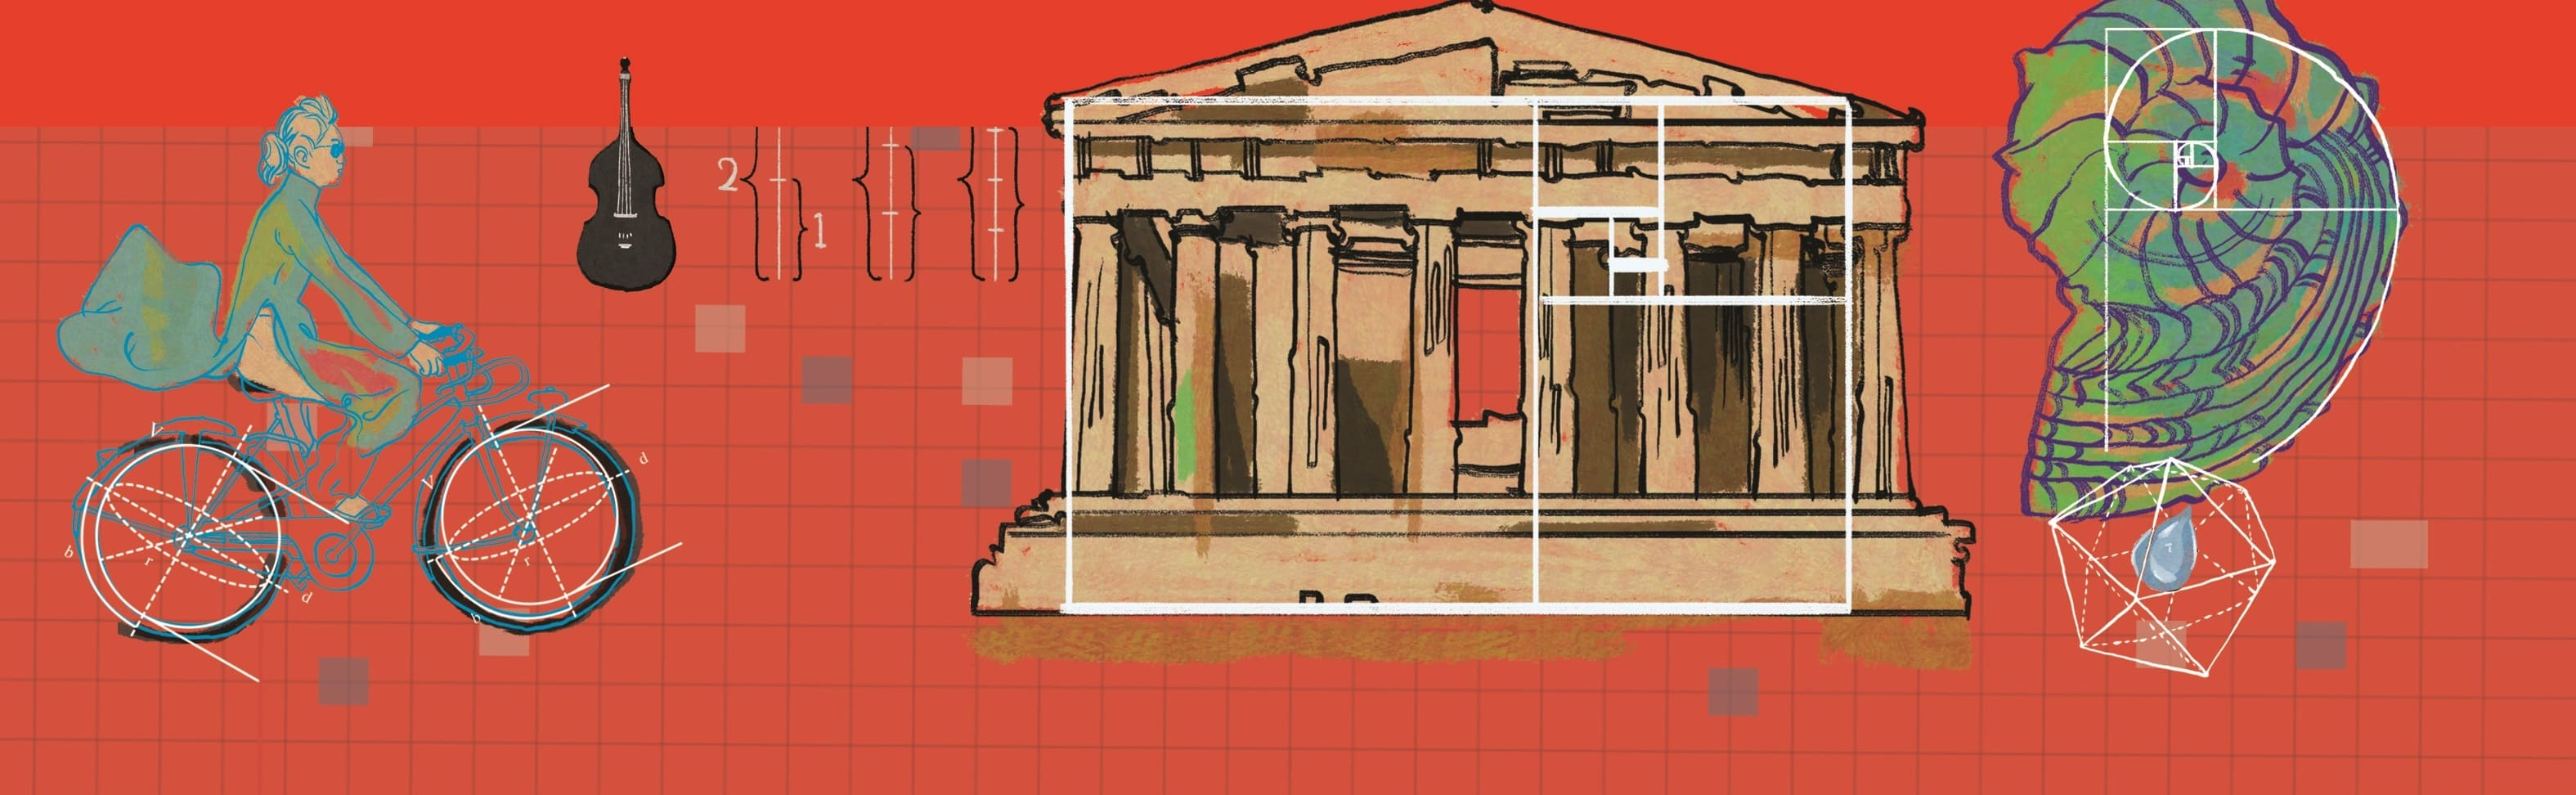
\includegraphics[width=19.3cm]{../bannertoanhocdoisong}}}
\AddToShipoutPicture*{\put(55,523){
\includegraphics[scale=1]{../tieude2.pdf}}}
\centering
\endgroup

\vspace*{188pt}
\begin{multicols}{2}
	Cuộc cách mạng công nghiệp lần thứ tư (sau đây gọi tắt là CMCN $4{.}0$) với xu hướng phát triển dựa trên nền tảng tích hợp cao độ của hệ thống kết nối Số hóa -- Vật lý -- Sinh học và sự đột phá của Internet vạn vật, Trí tuệ nhân tạo đang tác động đến toàn thế giới. Cuộc cách mạng này được dự báo sẽ xóa nhòa khoảng cách giữa thế giới thực với thế giới ảo. Đặc biệt, mức độ ảnh hưởng, lan tỏa của cuộc cách mạng này sẽ nhanh hơn những gì đã xảy ra từ trước đến nay và làm thay đổi toàn bộ hệ thống sản xuất, quản lý, quản trị trên toàn thế giới. Cuộc cách mạng công nghiệp lần thứ nhất bắt đầu vào khoảng nửa sau thế kỷ thứ $18$ với nền tảng là máy móc cơ khí vận hành bằng động cơ hơi nước.
	\begin{figure}[H]
		\vspace*{-5pt}
		\centering
		\captionsetup{labelformat= empty, justification=centering}
		
\includegraphics[width= 1\linewidth]{1a}
		\vspace*{-15pt}
	\end{figure}
	Cuộc cách mạng công nghiệp lần thứ hai vào khoảng nửa cuối thế kỷ thứ $19$ với nền tảng là động cơ đốt trong, động cơ điện và sản xuất theo dây chuyền. Cuộc cách mạng công nghiệp lần thứ ba được bắt đầu vào những năm $1960$ với nền tảng là công nghệ bán dẫn, điện tử, máy tính, tự động hóa. Cuộc cách mạng công nghiệp lần thứ tư được kế thừa từ Cuộc  cách mạng công nghiệp lần thứ ba và được đề cập nhiều từ những năm $2013$ với ba trụ cột chính là Kỹ thuật số, Sinh học và Vật lý.
	\vskip 0.05cm
	\textbf{\color{toanhocdoisong}Những đặc điểm nổi bật của CMCN $\pmb{4{.}0}$}
	\vskip 0.05cm
	Công nghệ trong kỷ nguyên CMCN $4{.}0$ có mức độ tự động hóa rất cao (so với mức độ tự động hóa của CMCN $3.0$), mô phỏng trí tuệ của con người. Trí tuệ nhân tạo (Artificial intelligence--AI) có thể tương tác với con người, thực hiện các hành vi thông minh như con người. Dựa trên các mô hình toán học và thuật toán phân tích dữ liệu lớn, AI có thể thay thế con người phân tích, tối ưu hóa, đưa ra quyết định và giải quyết vấn đề thay thế con người trong nhiều lĩnh vực, kể cả những lĩnh vực trước đây là độc quyền của con người như sáng tạo nghệ thuật v.v. 
	\vskip 0.05cm
	Công nghệ sinh học, công nghệ vật liệu trong CMCN $4.0$ có những bước tiến mang tính nhảy vọt, đột phá là nền tảng để tạo nên những tiến bộ vượt bậc trong lĩnh vực nông nghiệp, y học, dược liệu, năng lượng tái tạo… Vật lý hướng phát triển mạnh về nghiên cứu, chế tạo trang thiết bị công nghệ.
	\vskip 0.05cm
	Chuyển hóa thông tin từ thế giới thực (bao gồm cả các thực thể vật lý, xã hội và sinh học) sang thế giới ảo với dung lượng thông tin rất lớn, tốc độ cao và đa dạng về mọi mặt của đời sống tự nhiên và xã hội gắn với thuật ngữ chuyên môn là ``Dữ liệu lớn -- Big data". 
	\vskip 0.05cm
	Thông tin trong thế giới vật lý ảo này được kết nối với nhau và được quản lý, khai thác sử dụng bằng những hệ thống công nghệ số liên kết để xóa nhòa ranh giới không gian địa lý trên phạm vi toàn cầu và với tốc độ thời gian thực. Chúng ta luôn có được cái nhìn từ tổng quát toàn diện đến chi tiết thế giới hiện tại. Đây có thể coi là lời giải thích cho cụm từ chuyển đổi số hay nói cách khác chuyển đổi số là một xu hướng tất yếu của CMCN $4{.}0$.
	\vskip 0.05cm
	\textbf{\color{toanhocdoisong}Thế nào là chuyển đổi số (CĐS)}
	\vskip 0.05cm
	Khía cạnh công nghệ của CĐS là số hóa dữ liệu và ứng dụng dữ liệu dựa trên nền tảng kỹ thuật số. Công nghệ ở đây được hiểu là một hệ thống, trong đó có trang thiết bị kỹ thuật số, có các hệ thống xử lý kỹ thuật số, có dữ liệu đầu vào ở dạng số, có yêu tố con người, có yếu tố phương thức tổ chức hoạt động,  liên kết, tác động qua lại lẫn nhau và cho kết quả đầu ra là những sản phẩm có hiệu suất lớn về giá trị.
	\vskip 0.05cm
	Tuy nhiên với CĐS ở nghĩa rộng thì công nghệ không phải là yêu tố chính, mà là yếu tố kích thích. CĐS trong CMCN $4{.}0$ là quá trình hoàn chỉnh áp dụng số hóa và ứng dụng số hóa ở một cấp độ cao hơn và có quy mô lớn, là quá trình thay đổi phương thức kiến tạo, quản lý, điều hành, sử dụng dữ liệu truyền thống sang một phương thức kiến tạo, quản lý, điều hành, sử dụng dữ liệu dựa trên những nền tảng kỹ thuật số mới như: Dữ liệu lớn, Internet vạn vật, Trí tuệ nhân tạo, Điện toán đám mây, dựa vào lực lượng sản xuất mới, tiến bộ như đề cập ở trên trong mọi mặt trong đời sống xã hội với mục tiêu tạo nên một bước chuyển lớn về năng suất lao động và tổng giá trị sản xuất cho xã hội theo hướng bền vững và tích cực. Tóm lại CĐS trong CMCN $4{.}0$ là từ lực lượng sản xuất tiến bộ hiện đại, hình thành quan hệ sản xuất mới, phù hợp với mục tiêu xây dựng xã hội thịnh vương, hạnh phúc và tiến bộ. 
	\vskip 0.05cm
	\textbf{\color{toanhocdoisong}Chuyển đổi số ở nước ta}
	\vskip 0.05cm
	Tại Việt Nam, Đảng và Nhà nước ta đã sớm nhìn thấy cơ hội của CMCN $4{.}0$ và đã ban hành nhiều văn bản quan trong về chủ động tham gia vào CMCN $4{.}0$ (tiêu biểu là Nghị quyết $52$ của Bộ Chính trị năm $2019$ về một số chủ trương, chính sách chủ động tham gia cuộc Cách mạng công  nghiệp lần thứ tư; Quyết định $749$ của Thủ tướng Chính phủ phê duyệt Chương trình Chuyển đổi số quốc gia đến năm $2025$ định hướng đến năm $2030$). Chương trình chuyển đổi số quốc gia theo Quyết định $749$ nhằm xây dựng ba trụ cột chính là Chính phủ số, Xã hội số và Kinh tế số.
	\vskip 0.05cm
	Hiện nay, cả trong công tác xây dựng/thực hiện chính sách lẫn trong hoạt động thực tiễn khái niệm CĐS đã trở nên phổ biến, lan tỏa trên toàn xã hội. Trong đó, doanh nghiệp và cơ quan quản lý nhà nước là những tổ chức tiên phong và xem CĐS là xu thế bắt buộc, tất yếu để nâng cao hiệu quả sản xuất kinh doanh, sức cạnh tranh và thực hiện thành công chiến lược xây dựng chính quyền số gắn với cải cách hành chính, xây dựng nền kinh tế số và xã hội thông minh trong thời kỳ cách mạng công nghiệp $4{.}0$.
	\vskip 0.05cm
	CĐS đối với doanh nghiệp và các cơ quan quản lý nhà nước giúp xây dựng nên những dữ liệu/tài nguyên số tạo thuận lợi cho việc quản lý, khai thác sử dụng. Dữ liệu số hóa đã trở thành tài sản của các doanh nghiệp và các cơ quan quản lý nhà nước. Dữ liệu ngày càng được bổ sung, liên kết, tích hợp với nhau giúp cải thiện, tăng cường hiệu năng quản lý nhà nước, quản trị xã hội theo hướng công khai, minh bạch, hiệu quả, tạo ra những thay đổi lớn trong chuỗi giá trị hàng hóa và cung ứng sản phẩm; tự động hóa, nâng cao hiệu suất công việc, hiệu quả sản xuất kinh doanh, năng lực cạnh tranh, gia tăng mạnh mẽ giá trị sản xuất, chất lượng dịch vụ công.
	\vskip 0.05cm
	Ví dụ việc tạo lập dữ liệu về dân cư, dữ liệu về tư pháp, dữ liệu về doanh nghiệp, người nộp thuế ... và kết nối liên thông những dữ liệu này sẽ giúp người dân, doanh nghiệp thực hiện những dịch vụ công được nhanh chóng, thuận tiện, không phải xuất trình nhiều loại giấy tờ liên quan khi có nhu cầu sử dụng dịch vụ hành chính công, trong khi vẫn bảo đảm được quyền riêng tư về cá nhân. Các dịch vụ công trực tuyến về y tế, giáo dục, tư pháp, hải quan, thuế, đăng ký kinh doanh ... sẽ cung cấp cho người dân, doanh nghiệp những tiện ích nhanh chóng, hạn chế tiếp xúc trực tiếp (tránh tiêu cực và giảm thiểu chi phí đi lại) với cơ quan hành chính trong công việc, cuộc sống và hoạt động sản xuất, kinh doanh của mình, trong khi vẫn tuân thủ các thủ tục hành chính theo quy định của pháp luật. Việc xây dựng chính phủ số trong đó lấy người dân là đối tượng phục vụ và dựa vào dữ liệu số sẽ góp phần tăng cường hiệu lực, hiệu quả quản lý nhà nước. Mặt khác, tiến trình này giúp đẩy mạnh sự phát triển công nghệ thông tin, công nghệ số trong nước, giúp phát triển cộng đồng doanh nghiệp công nghệ và nguồn nhân lực công nghệ có chất lượng ở nước ta.
	\vskip 0.05cm
	Các doanh nghiệp, khi áp dụng CĐS và tham gia vào nền kinh tế số sẽ xây dựng được các cách thức quản trị mới, hiệu quả hơn dựa vào tạo lập và khai thác nguồn thông tin số hóa. Họ cũng sẽ tiếp cận khách hàng và mở rộng thị trường nhanh hơn nhờ áp dụng thương mại điện tử và các chiến lược marketing tiên tiến dựa vào công nghệ phân tích dữ liệu lớn về xu hướng thị trường và nhu cầu ngày càng đa dạng của các tầng lớp khách hàng trong một xã hội số năng động và biến đông liên tục.
	\vskip 0.05cm
	Có thể khẳng định, CMCN $4{.}0$ và xu thế chuyển đổi số là tất yếu. Nó tạo ra vô vàn cơ hội cho mọi quốc gia, mọi đối tượng. Tuổi trẻ Việt Nam, đang được sống trong một đất nước năng động, hội nhập cần khẩn trương trang bị cho mình kiến thức và quyết tâm nắm bắt cơ hội, giành tấm vé lên chuyến tàu CMCN $4{.}0$ đang chuyển động cực kỳ nhanh này.
\end{multicols}
\vspace*{-10pt}
\rule{1\linewidth}{0.1pt}
\begingroup
\blfootnote{$^1$\color{toanhocdoisong}Hà Nội.}

\AddToShipoutPicture*{\put(100,268){
\includegraphics[scale=1]{../tieude3.pdf}}}
\centering
\endgroup

\vspace*{45pt}

\begin{multicols}{2}
	Mã QR đã trở nên rất quen thuộc trong đời sống hàng ngày quanh ta, mang lại sự tiện lợi lớn cho các hoạt động giao dịch cũng như trao đổi thông tin. Trong bài này, chúng ta hãy cùng tìm hiểu về vai trò của toán học trong quá trình xây dựng loại mã này.
	\vskip 0.05cm
	$\pmb{1.}$ \textbf{\color{toanhocdoisong}\color{toanhocdoisong}Mã sửa lỗi và sự ra đời của mã Reed -- Solomon}
	\vskip 0.05cm
	Một vấn đề không tránh khỏi khi thông tin được truyền tải từ nơi này đến nơi khác là việc nó có thể bị sai lệch trong quá trình truyền tin. Với các tín hiệu dạng nhị phân, một bit $0$ có thể biến thành $1$ và ngược lại. Xác suất của việc này phụ thuộc vào các đặc tính của đường truyền cũng như môi trường truyền dẫn.
	\vskip 0.05cm
	Để đảm bảo thông tin có thể được kiểm chứng đúng/sai, ta cần ghi thông tin theo một loại mã có thể giúp ta khẳng định nó có bị lỗi hay không. Loại mã này gọi là mã phát hiện lỗi.
	\vskip 0.05cm
	Một ví dụ về mã phát hiện lỗi là mã số của sách (ISBN) hoặc tạp chí (ISSN). Tạp chí Pi của chúng ta có mã ISSN là $2525-2437$. Trong $8$ chữ số của mã, chữ số cuối cùng được dùng để phát hiện lỗi. Đầu tiên, ta lấy $7$ chữ số đầu tiên, nhân mỗi một chữ số với số thứ tự tính từ bên phải (tức là $8$, $7$, $6$, $5$, ..., $2$) rồi tính tổng:
	\setlength{\abovedisplayskip}{4pt}
	\setlength{\belowdisplayskip}{4pt}
	\begin{align*}
		&2\times8+5\times7+2\times6+5\times5+2\times4\\
		&+4\times3+3\times2=114.
	\end{align*}
	Lấy tổng này chia cho $11$ rồi lại lấy $11$ trừ đi số dư sẽ được chữ số cuối cùng (nếu giá trị này là $10$ thì ký tự cuối cùng là $X$; nếu số dư là $0$ thì chữ số cuối cùng là $0$): $114$ chia $11$ dư $4$; $11 - 4 = 7$.
	\vskip 0.05cm
	Nếu chữ số hoặc ký tự cuối không khớp với $7$ chữ số đầu tiên, ta có thể khẳng định rằng ISSN đã bị nhập sai. Cách làm này không chỉ phát hiện lỗi do một vị trí bị thay đổi mà còn phát hiện được trường hợp hai vị trí cạnh nhau bị hoán vị (một lỗi thường thấy khi con người nhập dữ liệu) thông qua hệ số khác nhau của các vị trí. Số $11$ được chọn do nó là một số nguyên tố, không chia hết cho bất cứ hệ số nào trong phép nhân. Nếu ta chọn số $10$, nó sẽ không phát hiện được lỗi nếu chữ số ở vị trí $5$ bị thay đổi một lượng chẵn.
	\vskip 0.05cm
	Trong nhiều trường hợp, chỉ phát hiện được lỗi là không đủ. Thay vì yêu cầu tín hiệu được gửi lại khi có lỗi, người ta muốn sử dụng một loại mã có thể giúp sửa lỗi khi lỗi được phát hiện. Muốn vậy, khi gửi tín hiệu, ta cần thêm một số thông tin khác để trợ giúp sửa lỗi.
	\vskip 0.05cm
	Một cách đơn giản nhất là gửi thông tin lặp. Thay vì gửi một bit có giá trị là $0$ hoặc $1$, ta có thể gửi nhiều bit có cùng giá trị. Chẳng hạn, nếu tín hiệu nhận được là $1101110111$, với quy định là $10$ bit liền nhau sẽ có cùng một giá trị, thì ta có thể khẳng định bit được gửi đi là $1$. Cách làm đơn giản này tuy có thể giúp sửa lỗi nhưng nó rất lãng phí đường truyền.
	\vskip 0.05cm
	Vậy cần phải truyền thêm bao nhiêu dữ liệu và dữ liệu sửa lỗi cần phải có dạng như thế nào? Đây là những vấn đề thiết yếu của ngành lý thuyết mã.
	\vskip 0.05cm
	Năm $1948$, những nghiên cứu của nhà toán học Claude Shannon về entropy của thông tin cùng lượng thông tin cần truyền tối thiểu để sửa lỗi đã thúc đẩy nhiều nghiên cứu về các phương thức truyền thông tin có sửa lỗi.
	\vskip 0.05cm
	Một loại mã sửa lỗi quan trọng ra đời vào những năm $1950$ là mã Hamming (theo tên của nhà toán học R. W. Hamming). Ta hãy xét một trường hợp rất đơn giản với dữ liệu được truyền theo $3$ bit một, với $8$ tổ hợp: $000$, $001$, $010$, $011$, $100$, $101$, $110$, $111$. Nếu ta chọn cả $8$ tổ hợp này để truyền tin thì khi có một bit bị lỗi, ta không thể tiến hành phát hiện lỗi. Một cách đơn giản là chọn các trạng thái mà khi bị lỗi, ta có thể biết được giá trị gốc của tín hiệu.
	\begin{figure}[H]
		\vspace*{-10pt}
		\centering
		\captionsetup{labelformat= empty, justification=centering}
		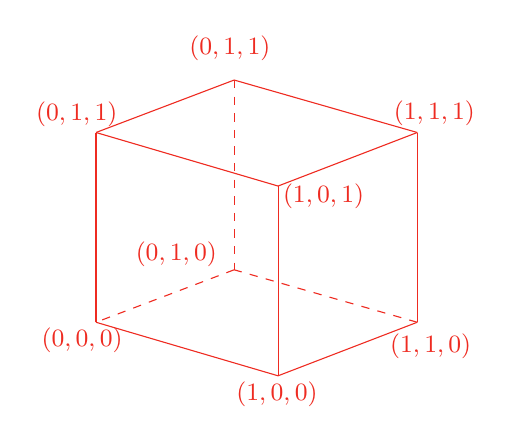
\begin{tikzpicture}[toanhocdoisong,scale=0.68, node font=\small]
			\draw [] (-2.,1.)-- (1.4,0.);
			\draw [] (1.4,0.)-- (4.,1.);
			\draw [dashed] (4.,1.)-- (0.58,1.98);
			\draw [dashed] (0.58,1.98)-- (-2.,1.);
			\draw [] (-2.,1.)-- (-2.,4.5440090293338695);
			\draw [] (-2.,4.5440090293338695)-- (0.58,5.524009029333869);
			\draw [] (0.58,5.524009029333869)-- (4.,4.54400902933387);
			\draw [] (4.,4.54400902933387)-- (1.4,3.5440090293338695);
			\draw [] (1.4,3.5440090293338695)-- (-2.,4.5440090293338695);
			\draw [] (1.4,3.5440090293338695)-- (1.4,0.);
			\draw [] (4.,4.54400902933387)-- (4.,1.);
			\draw [dashed] (0.58,5.524009029333869)-- (0.58,1.98);
			\draw (-2.26,0.67) node {$(0,0,0)$};
			\draw (1.38,-0.35) node {$(1,0,0)$};
			\draw (4.25,0.55) node {$(1,1,0)$};
			\draw (-0.5,2.27) node {$(0,1,0)$};
			\draw (-2.36,4.89) node {$(0,1,1)$};
			\draw (0.5,6.11) node {$(0,1,1)$};
			\draw (2.25,3.35) node {$(1,0,1)$};
			\draw (4.32,4.91) node {$(1,1,1)$};
		\end{tikzpicture}
		
		\vspace*{-5pt}
		\caption{\small\textit{\color{toanhocdoisong}Hình $1$. Các tổ hợp $3$ bit nhị phân biểu diễn theo dạng hình lập phương. Các đỉnh kề nhau sẽ khác biệt một bit.}}
		\vspace*{-10pt}
	\end{figure}
	Ta hãy biểu diễn $8$ tổ hợp trên $8$ đỉnh của hình lập phương. Có thể thấy khi đi từ một đỉnh đến một đỉnh kề nó thì có đúng một bit bị thay đổi. Số cạnh trên đường đi từ một đỉnh đến một đỉnh khác cho ta biết số bit bị thay đổi giữa hai trạng thái. Đây được gọi là khoảng cách Hamming giữa chúng. Ví dụ khoảng cách Hamming giữa $000$ và $101$ là $2$ còn khoảng cách giữa $000$ và $111$ là $3$.
	\vskip 0.05cm
	Giả sử trong môi trường truyền tin, tín hiệu $3$ bit bị lỗi tối đa một bit. Để có thể xác định được trạng thái gốc từ trạng thái lỗi, ta chỉ có thể chọn các đỉnh có khoảng cách là $3$. Do đó, chỉ có thể chọn $2$ đỉnh là $000$ và $111$. Giả sử tín hiệu nhận được là $011$, ta sẽ biết được tín hiệu gốc là $111$ do khoảng cách Hamming giữa chúng là $1$ còn khoảng cách Hamming giữa $011$ và $000$ là $2$. Khi đó, $000$ và $111$ được gọi là các từ mã (codeword) cho việc truyền tín hiệu. Trong trường hợp này ta truyền đi tổng cộng $3$ bit nhưng lượng thông tin chỉ có $1$ bit (ứng với $2^1$ từ mã) cho nên hiệu suất truyền của ta là $1/3$. Nếu chọn tập hợp các đỉnh có khoảng cách giữa chúng là $2$ (ví dụ $4$ đỉnh $000$, $011$, $101$, $110$) để làm từ mã thì ta chỉ có thể phát hiện lỗi chứ không sửa lỗi (ví dụ $001$ có khoảng cách đến $000$ và $011$ đều là $1$).
	\begin{table}[H]
		\vspace*{-5pt}
		\centering
		\captionsetup{labelformat= empty, justification=centering}
		\begin{tabular}{c c c c c c c c}
			\hline
			$1$ &$0$&$0$&$0$&$0$&$0$&$0$&$0$\\
			$2$ &$1$&$1$&$1$&$0$&$0$&$0$&$0$\\
			$3$ &$1$&$0$&$0$&$1$&$1$&$0$&$0$\\
			$4$ &$0$&$1$&$1$&$1$&$1$&$0$&$0$\\
			$5$ &$0$&$1$&$0$&$1$&$0$&$1$&$0$\\
			$6$ &$1$&$0$&$1$&$1$&$0$&$1$&$0$\\
			$7$ &$1$&$1$&$0$&$0$&$1$&$1$&$0$\\
			$8$ &$0$&$0$&$1$&$0$&$1$&$1$&$0$\\
			$9$ &$1$&$1$&$0$&$1$&$0$&$0$&$1$\\
			$10$ &$0$&$0$&$1$&$1$&$0$&$0$&$1$\\
			$11$ &$0$&$1$&$0$&$0$&$1$&$0$&$1$\\
			$12$ &$1$&$0$&$1$&$0$&$1$&$0$&$1$\\
			$13$ &$1$&$0$&$0$&$0$&$0$&$1$&$1$\\
			$14$ &$0$&$1$&$1$&$0$&$0$&$1$&$1$\\
			$15$ &$0$&$0$&$0$&$1$&$1$&$1$&$1$\\
			$16$ &$1$&$1$&$1$&$1$&$1$&$1$&$1$\\
			\hline
		\end{tabular}	
		\caption{\small\textit{\color{toanhocdoisong}Bảng $1$. $16$ từ mã độ dài $7$ bit.}}
		\vspace*{-10pt}
	\end{table}
	Với mã Hamming, các quy tắc tính chẵn lẻ được tận dụng để thêm vào các thông tin cho phép sửa lỗi. Ta hãy xét một mã Hamming đơn giản với $7$ bit $b_1,b_2,\ldots,b_7$ theo quy tắc sau:
	\vskip 0.05cm
	$\bullet$ $b_1+b_3+b_5+b_7$ là chẵn
	\vskip 0.05cm
	$\bullet$ $b_2+b_3+b_6+b_7$ là chẵn
	\vskip 0.05cm
	$\bullet$ $b_4+b_5+b_6+b_7$ là chẵn
	\vskip 0.05cm
	Có tổng cộng $16$ từ mã độ dài $7$ bit thỏa mãn các quy tắc trên (Bảng $1$). Đồng thời, các từ mã này đều có khoảng cách Hamming giữa chúng là $3$.
	
	Khi giải mã tín hiệu, các tín hiệu vi phạm những quy tắc chẵn lẻ sẽ bị coi là lỗi. Việc phát hiện lỗi nằm ở bit nào (giả sử chỉ có $1$ bit bị lỗi) thì phức tạp hơn một chút. Tuy ta có thể dò xem từ mã nào có khoảng cách ngắn nhất đến tín hiệu bị lỗi, việc này khá mất thời gian. Thay vì đó, người ta sử dụng dạng ma trận của các quy tắc được sử dụng để xây dựng mã (Bảng $2$).
	\begin{table}[H]
		\vspace*{-5pt}
		\centering
		\captionsetup{labelformat= empty, justification=centering}
		\begin{tabular}{ccccccc}
			\hline
			$b_1$ & $b_2$& $b_3$& $b_4$&$b_5$ &$b_6$ &$b_7$\\
			\hline
			$1$ & $0$&$1$&$0$&$1$&$0$&$1$\\
			$0$ & $1$&$1$&$0$&$0$&$1$&$1$\\
			$0$ & $0$&$0$&$1$&$1$&$1$&$1$\\
		\end{tabular}	
		\caption{\small\textit{\color{toanhocdoisong}Bảng $2$. Ma trận ứng với $3$ quy tắc trong mã Hamming mà ta đang xét.}}
		\vspace*{-10pt}
	\end{table}
	Ví dụ, với chuỗi tín hiệu lỗi $1101101$, nó vi phạm quy tắc $1$ và $3$. Ta cần tìm cột trong ma trận mà khi bit ứng với cột này bị lật ngược lại thì chỉ có quy tắc $1$ và $3$ bị ảnh hưởng còn quy tắc $2$ không thay đổi. Nói cách khác, ta cần tìm cột có dạng:
	\begin{align*}
		1\\[-0.5ex]
		0\\[-0.5ex]
		1
	\end{align*}
	tức là cột thứ $5$ trong ma trận. Do đó, có thể kết luận bit thứ $5$ bị lỗi và từ mã gốc là $1101001$.
		\begin{figure}[H]
		\vspace*{-5pt}
		\centering
		\captionsetup{labelformat= empty, justification=centering}
		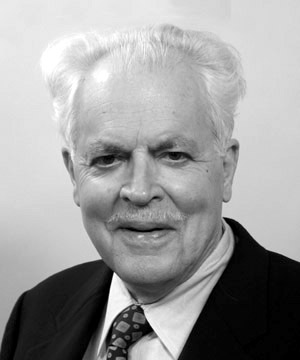
\includegraphics[height= 0.575\linewidth]{2}
		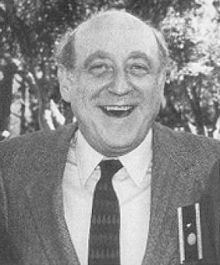
\includegraphics[height= 0.575\linewidth]{3}
		\caption{\small\textit{\color{toanhocdoisong}Trái: Irving Reed ($1923 - 2012$). Phải: Gustave Solomon ($1930 - 1996$).}}
		\vspace*{-10pt}
	\end{figure}
	Mã Hamming $7$ bit trên có $2^4=16$ từ mã, tức là khi truyền đi $7$ bit, ta thu được lượng thông tin tương đương với $4$ bit. Hiệu suất truyền ở đây là $4/7$. Tùy theo nhu cầu, người ta có thể thiết kế các mã Hamming với khoảng cách giữa các từ mã lớn hơn để có thể sửa lỗi cho nhiều hơn $1$ bit.
	\vskip 0.05cm
	Sau khi Hamming đưa ra mã sửa lỗi thực tiễn đầu tiên sử dụng các kỹ thuật đại số tuyến tính như trên, cuộc đua giữa các nhà toán học để tìm ra những cách mã hóa tốt hơn trở nên sôi động. Một dấu ấn quan trọng của ngành mã hóa là sự ra đời của mã Reed -- Solomon, được hai nhà toán học Irving Reed và Gustave Solomon công bố năm $1960$. Mã này sử dụng các cấu trúc đại số phức tạp hơn bao gồm trường Galois cùng các đa thức trên trường này (xem chi tiết ở phần phụ lục). Với nhiều lợi thế so với mã Hamming về khả năng sửa lỗi cũng như hiệu suất truyền, mã Reed -- Solomon đã có nhiều ứng dụng rộng rãi trong các lĩnh vực của đời sống. Một trong số những ứng dụng đó chính là mã QR. 
	\vskip 0.05cm
	$\pmb{2.}$ \textbf{\color{toanhocdoisong}\color{toanhocdoisong}Mã QR}
%	\vskip 0.05cm
	\begin{figure}[H]
			\vspace*{-5pt}
			\centering
			\captionsetup{labelformat= empty, justification=centering}
			
\includegraphics[width= 0.7\linewidth]{QR}
			\caption{\small\textit{\color{toanhocdoisong}Hình $2$. Mã QR của Tạp chí Pi.}}
			\vspace*{-10pt}
		\end{figure}
	Mã QR (viết tắt của Quick Response) mà chúng ta quen thuộc được kỹ sư người Nhật, Masahiro Hara thiết kế năm $1994$ khi làm tại công ty Denso Wave. Lúc đó, Masahiro được giao nhiệm vụ thiết kế một loại mã mới để thay thế mã vạch (barcode) (Hình $3$). Tuy mã vạch đã được dùng rất phổ biến trong cả sản xuất lẫn phân phối, nhưng vì nó ghi lại thông tin theo một chiều nên dung lượng thông tin của mã vạch ($20$ ký tự) đã không còn đáp ứng được nhu cầu thực tế với sự đa dạng hóa sản xuất đầu những năm $1990$ ở Nhật. Để lưu trữ những thông tin dài, người ta thường phải sử dụng nhiều mã vạch cùng lúc và do đó phải tiến hành quét nhiều lần cho mỗi sản phẩm.
	\begin{figure}[H]
		\vspace*{-10pt}
		\centering
		\captionsetup{labelformat= empty, justification=centering}
		$a)$
\includegraphics[width= 0.8\linewidth]{4}
		$b)$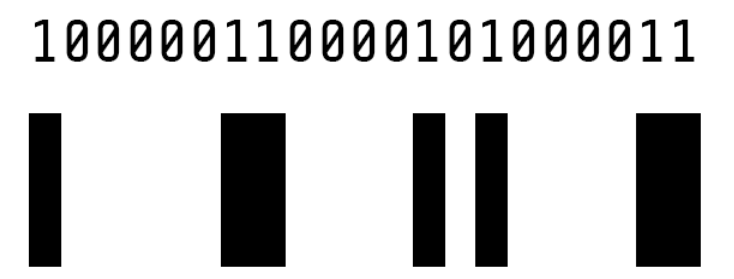
\includegraphics[width= 0.8\linewidth]{5}
		\caption{\small\textit{\color{toanhocdoisong}Hình $3.$ $a)$ Mã vạch gồm cách vạch với độ dày và khoảng cách khác nhau. $b)$ Thực chất của mã vạch là các cột màu trắng hoặc đen liên tiếp ứng với các bit $0$ hoặc $1$ để biểu diễn thông tin đã được chuyển từ dạng ký tự sang dạng bit.}}
		\vspace*{-10pt}
	\end{figure}
	Để có thể chứa được nhiều thông tin hơn, Masahiro quyết định sử dụng mã dạng hình vuông (hai chiều không gian thay vì một chiều như mã vạch). Vấn đề đầu tiên là làm thế nào để thiết bị có thể nhận diện được vùng mã khi quét. Masahiro đã nảy ra ý tưởng đưa thêm các hình hình học vào các góc để giúp định vị mã.
	\vskip 0.05cm
	Tuy nhiên, việc chọn các hình hình học này thế nào cũng là vấn đề khó bởi trong thực tế có thể có các hình hình học khác ở gần mã của ta làm phần mềm không thể nhận diện được mã một cách chính xác. Sau một thời gian nghiên cứu về tỷ lệ giữa các vùng trắng/đen trong các nội dung  ảnh hoặc văn bản trên báo, tạp chí, tờ rơi, thùng carton, và nhiều tài liệu khác, nhóm làm việc của Masahiro quyết định sử dụng hình ô vuông như ta thấy ở ba góc của mã QR ngày nay. Hình ô vuông này có tỷ lệ các phần đen/trắng khi quét theo các góc khác nhau đều là $1 : 1 : 3 : 1 : 1$. Theo kết quả thống kê thì tỷ lệ này ít xuất hiện nhất trên các vật liệu in thực tế nên mã QR sẽ không bị lẫn vào môi trường xung quanh và có thể được thiết bị quét nhận diện tự động nhanh chóng sau khi tiến hành quét.
	\begin{figure}[H]
		\vspace*{-10pt}
		\centering
		\captionsetup{labelformat= empty, justification=centering}
		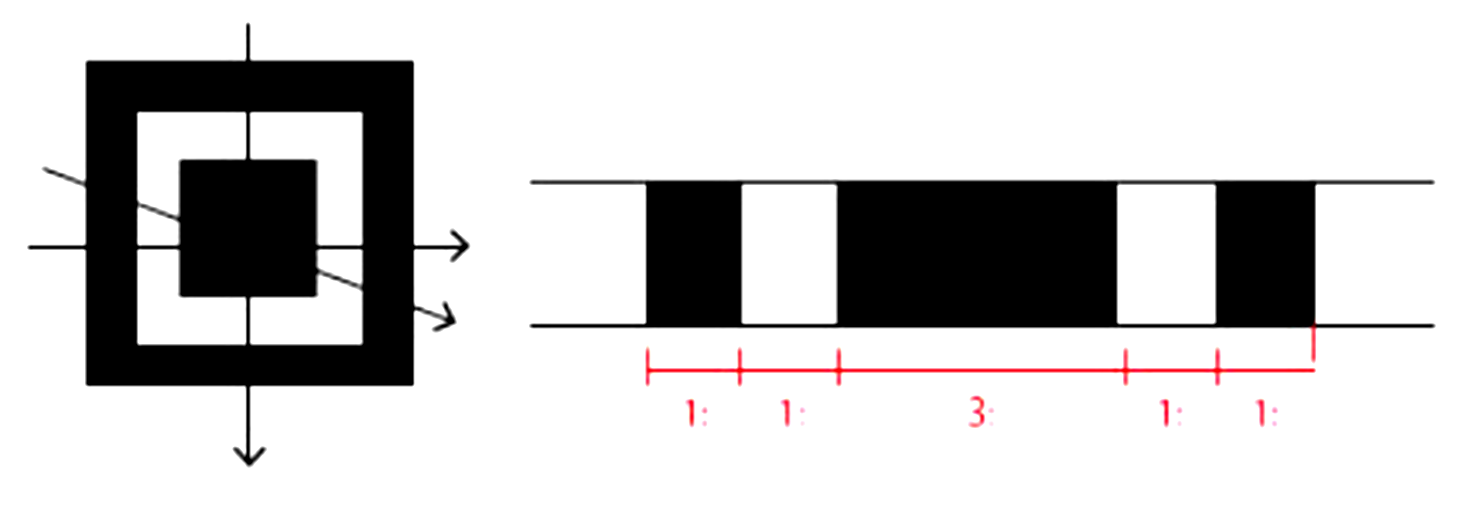
\includegraphics[width=1\linewidth]{6}
		\caption{\small\textit{\color{toanhocdoisong}Hình $4$. Ô vuông định vị cho mã QR và tỷ lệ đen/trắng khi quét.}}
		\vspace*{-10pt}
	\end{figure}
	Một vấn đề thực tế khác mà Masahiro muốn giải quyết với mã QR là tình trạng các vết bẩn làm sai lệch thông tin. Trong các môi trường như nhà xưởng, cửa hàng, mã đã in ra có thể dễ dàng bị dính các loại dầu, bụi đất, ... Để việc đọc mã có thể tiến hành thuận lợi trong các điều kiện này, ông sử dụng mã sửa lỗi Reed -- Solomon để ghi thông tin thay vì chuyển trực tiếp từ dạng ký tự sang dạng bit như mã vạch. Do đó, thông tin bị sai lệch ở mức độ cho phép trong quá trình quét có thể được sửa lại thay vì phải quét lại hoặc làm sạch vùng chứa mã.
	\begin{figure}[H]
		\vspace*{-5pt}
		\centering
		\captionsetup{labelformat= empty, justification=centering}
		$a)$
\includegraphics[height=0.35\linewidth]{7}
		$b)$
\includegraphics[height=0.35\linewidth]{8}
		$c)$
\includegraphics[height=0.35\linewidth]{9}
		$d)$
\includegraphics[height=0.35\linewidth]{10}
		\caption{\small\textit{\color{toanhocdoisong}Hình $5$. Một số thành phần của mã QR. $a)$ Các ô định vị. $b)$ Ô vuông gióng hàng. $c)$ Phần ghi dữ liệu. $d)$ Phần viền trắng.}}
		\vspace*{-10pt}
	\end{figure}
	Từ khi được Masahiro thiết kế đến nay, mã QR đã trải qua nhiều phiên bản. Về cơ bản, một mã QR gồm các nội dung như trong Hình $5$. Ngoài các ô vuông định vị và phần thông tin sử dụng mã Reed -- Solomon, mã QR còn gồm một số thành phần khác như ô vuông gióng hàng, phần viền trắng (để tách biệt với xung quanh) và các phần ghi một số thông tin khác về phiên bản mã và định dạng mã, v.v. 
	\begin{figure}[H]
		\vspace*{-5pt}
		\centering
		\captionsetup{labelformat= empty, justification=centering}
		
\includegraphics[height=0.35\linewidth]{11}
		
		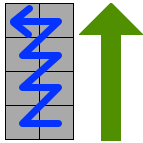
\includegraphics[height=0.33\linewidth]{12}
		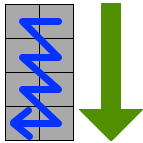
\includegraphics[height=0.33\linewidth]{13}
		\caption{\small\textit{\color{toanhocdoisong}Hình $6$. Thông tin sau khi được mã hóa theo mã Reed -- Solomon sẽ được ghi theo các làn như hình vẽ (trên). Ứng với mỗi chiều trong làn, thông tin sẽ được ghi trong hai cột (dưới) với màu đen đại diện bit $1$ còn màu trắng đại diện bit $0$.}}
		\vspace*{-10pt}
	\end{figure}
	Khi mã hóa, các thông tin thực tế (chữ số, ký tự, ...) đã được chuyển thành dạng bit nhị phân theo quy tắc định trước (tùy theo phiên bản mã QR) sẽ được mã hóa thành mã Reed -- Solomon dạng bit. Các bit được ghi lên trên hình vuông theo cách thức như trong Hình~$6$. Vị trí đen ứng với bit $1$ còn vị trí trắng ứng với bit $0$.
	
	Khi thiết bị quét mã QR, phần mềm sẽ định vị mã dựa vào vị trí của các ô vuông đánh dấu và tiến hành quét phần dữ liệu. Dữ liệu sau khi quét được tiến hành giải mã theo thuật toán giải mã của mã Reed -- Solomon. Do khả năng sửa lỗi của mã này nên nếu quá trình quét có một số bit bị nhận diện sai (đen thành trắng hoặc trắng thành đen), phần mềm vẫn có thể tiến hành sửa lỗi để cho ra thông tin ban đầu. Nếu số lượng lỗi vượt quá khả năng sửa lỗi của thuật toán, người dùng phải tiến hành quét lại.
	\begin{figure}[H]
		\vspace*{-5pt}
		\centering
		\captionsetup{labelformat= empty, justification=centering}
		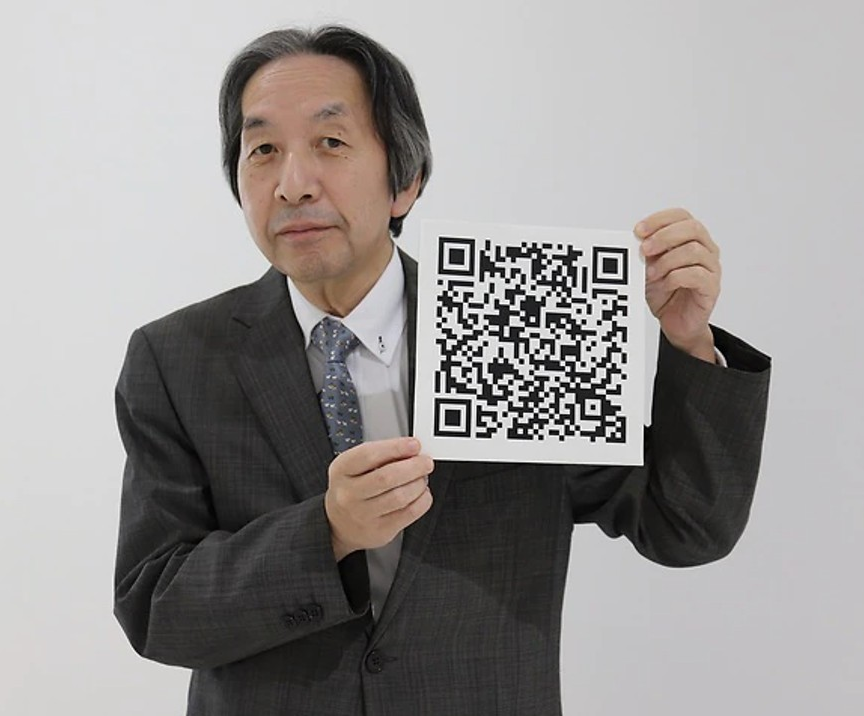
\includegraphics[width= 1\linewidth]{14}
		\caption{\small\textit{\color{toanhocdoisong}Hình $7a$. Masahiro và mã QR do ông phát minh.}}
		\vspace*{-5pt}
	\end{figure}
	\begin{figure}[H]
		\vspace*{5pt}
		\centering
		\captionsetup{labelformat= empty, justification=centering}
		
\includegraphics[width= 1\linewidth]{15}
		\caption{\small\textit{\color{toanhocdoisong}Hình $7b$. Masahiro có ý tưởng về các ô đen trắng cho mã QR từ trò chơi Go (cờ vây) mà ông hay chơi trong giờ nghỉ.}}
		\vspace*{-10pt}
	\end{figure}
	Ngày nay, với sự phổ biến của các thiết bị điện thoại thông minh, mã QR đã xuất hiện không chỉ ở trong các dây chuyền sản xuất mà còn được ứng dụng ở rất nhiều hoạt động của đời sống trên thế giới, từ thanh toán ngân hàng đến các giao dịch ở cửa hàng, siêu thị, bệnh viện, phương tiện công cộng, v.v. Nó cũng có vai trò quan trọng trong việc truy vết COVID $19$ ở nhiều nơi trên thế giới trong thời gian vừa qua; bản thân Masahiro cũng nói rằng ông cảm thấy rất hài lòng về sự đóng góp này của mã QR.
	\begin{figure}[H]
		\vspace*{-5pt}
		\centering
		\captionsetup{labelformat= empty, justification=centering}
		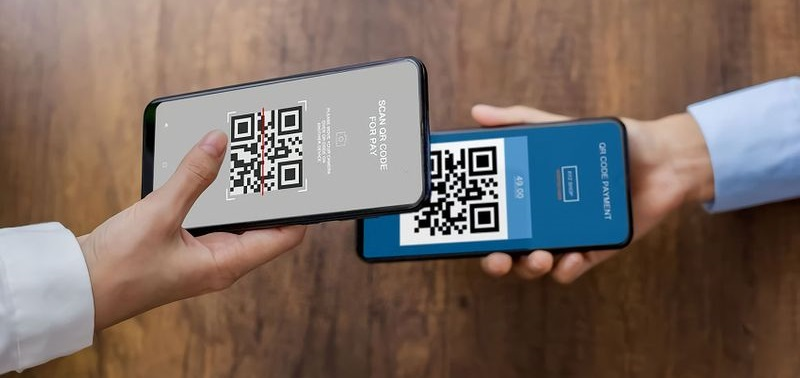
\includegraphics[width= 1\linewidth]{16}
		\caption{\small\textit{\color{toanhocdoisong}Hình $8$. Việc sử dụng mã QR giúp tiến hành các giao dịch không cần tiền mặt chỉ với điện thoại di động.}}
		\vspace*{-10pt}
	\end{figure}
	$\pmb{3.}$ \textbf{\color{toanhocdoisong}\color{toanhocdoisong}Một số ứng dụng khác của mã Reed -- Solomon}
	\vskip 0.05cm
	Mã Reed -- Solomon đã từ lâu được sử dụng để mã hóa dữ liệu cho các loại đĩa lưu trữ thường thấy trong đời sống như CD, DVD, MiniDisc và Blu--ray. Dữ liệu nhị phân sau khi chuyển thành mã Reed -- Solomon sẽ được ghi lên bề mặt đĩa tạo thành các rãnh lồi lõm. Khi đầu đọc đọc lại các bit này, chúng sẽ được giải mã theo thuật toán giải mã tương ứng để cho ra dữ liệu ban đầu. Do khả năng khôi phục lỗi của mã Reed -- Solomon, ngay cả khi có lỗi lúc đọc (thường do bề mặt đĩa bị bụi, bẩn, ...), hệ thống vẫn có thể khôi phục dữ liệu gốc.
	\begin{figure}[H]
		\vspace*{-5pt}
		\centering
		\captionsetup{labelformat= empty, justification=centering}
		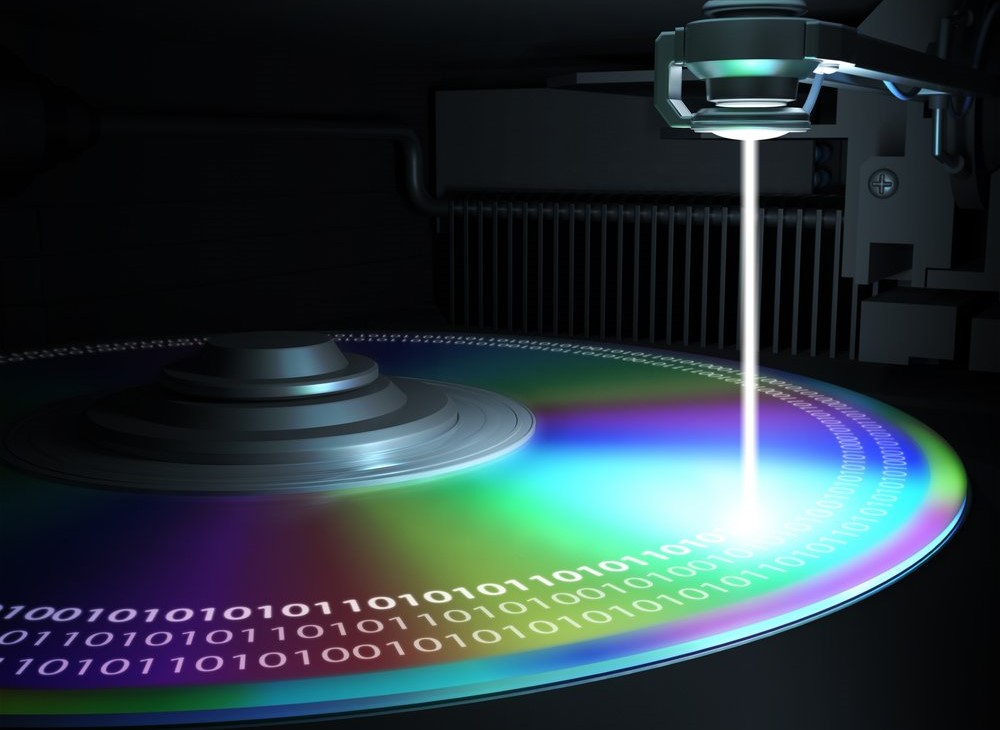
\includegraphics[width= 1\linewidth]{17}
		\caption{\small\textit{\color{toanhocdoisong}Hình $9$. Dữ liệu được mã hóa thành mã Reed - Solomon trước khi ghi trên bề mặt của các đĩa quang học.}}
		\vspace*{-10pt}
	\end{figure}
	Mã Reed -- Solomon cũng được sử dụng để mã hóa dữ liệu cho việc truyền tin của ngành viễn thông, theo dây cáp lẫn vô tuyến. Đặc biệt, mã này được sử dụng trên các thiết bị thăm dò không gian của NASA như tàu thăm dò Voyager $1$ và nhiều tàu thăm dò sau~đó.
	\begin{figure}[H]
		\vspace*{-5pt}
		\centering
		\captionsetup{labelformat= empty, justification=centering}
		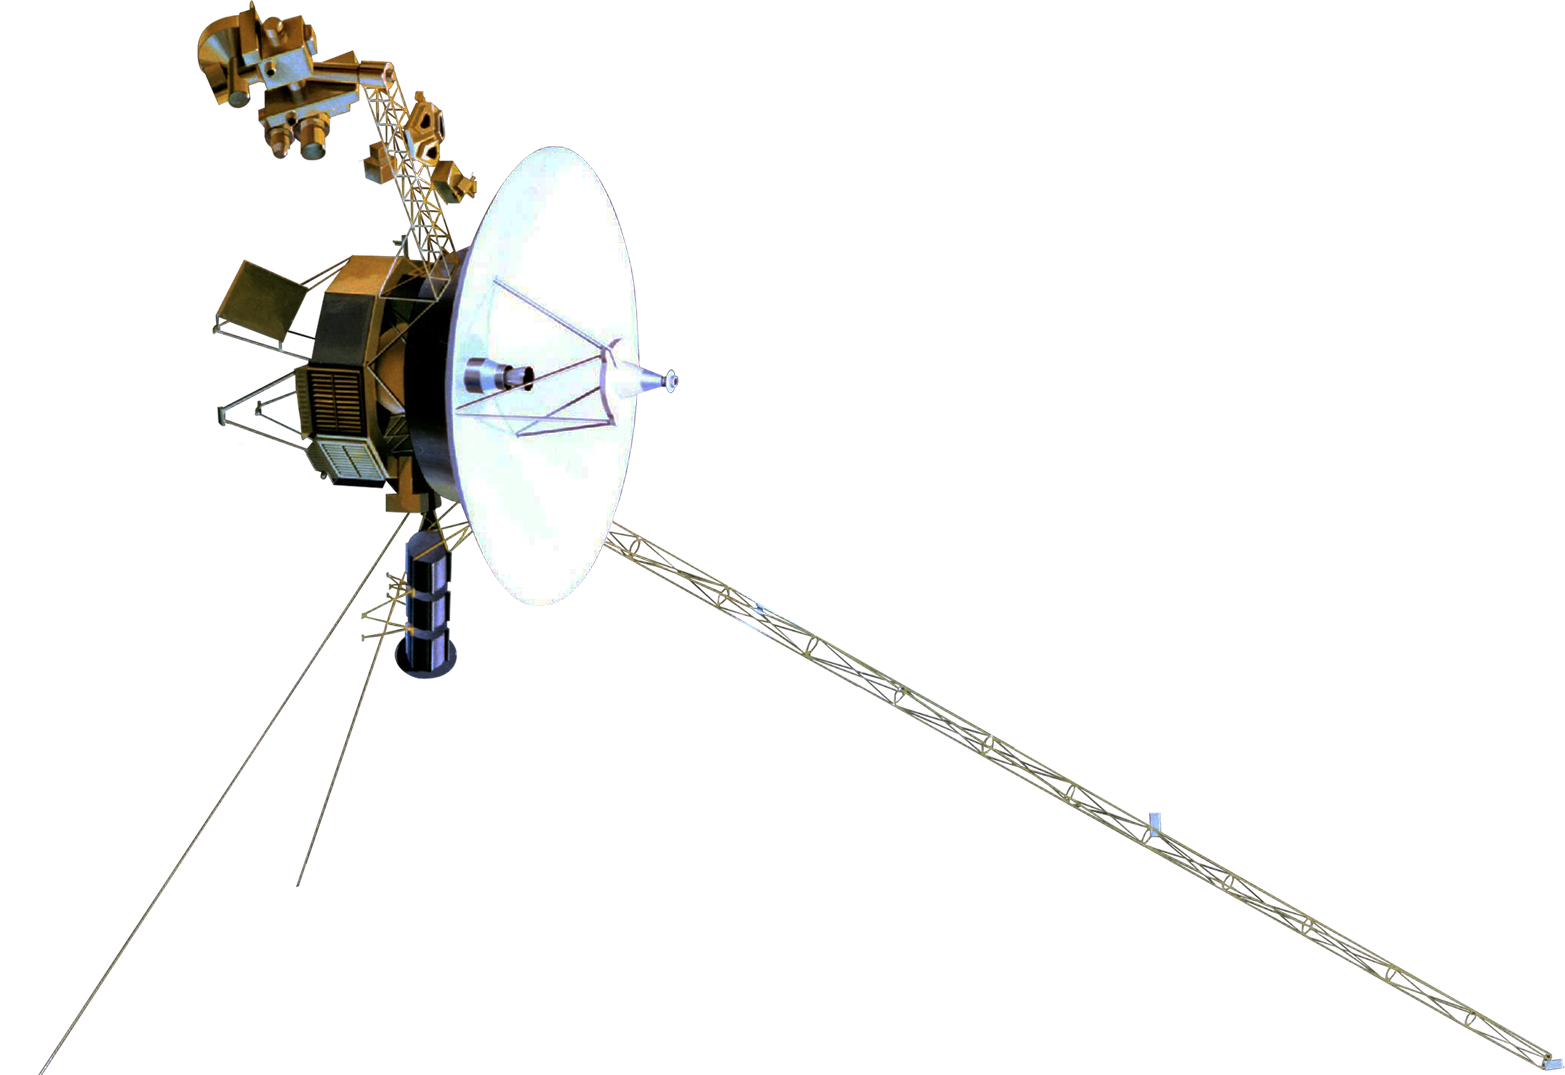
\includegraphics[width= 0.95\linewidth]{18}
		\caption{\small\textit{\color{toanhocdoisong}Hình $10$. Tàu thăm dò Voyager $1$ của NASA.}}
		\vspace*{-10pt}
	\end{figure}
	Mã Reed -- Solomon còn xuất hiện ở các hệ thống lưu trữ trong trung tâm dữ liệu. Trong kết nối ổ cứng theo dạng RAID $6$, các mã Reed -- Solomon để sửa lỗi cho dữ liệu của mỗi ổ cứng sẽ được hệ thống phân bố ở các ổ khác. Nếu một ổ cứng bị hỏng, dữ liệu có thể được khôi phục từ dữ liệu cùng các mã Reed -- Solomon ở trong các ổ cứng \linebreak còn lại. 
	\begin{figure}[H]
		\vspace*{-5pt}
		\centering
		\captionsetup{labelformat= empty, justification=centering}
		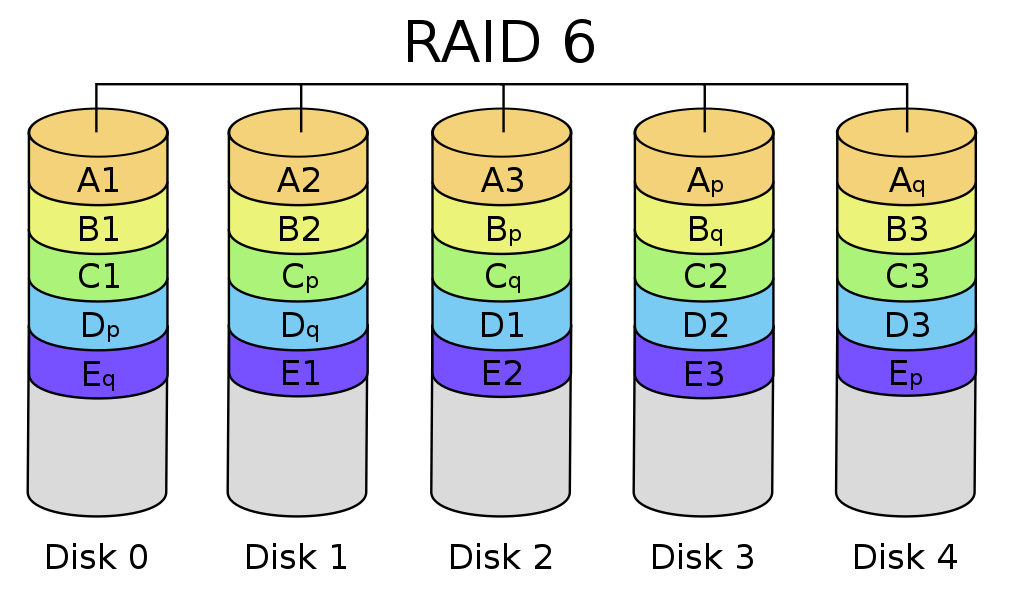
\includegraphics[width= 1\linewidth]{19}
		\caption{\small\textit{\color{toanhocdoisong}Hình $11$. Lưu trữ dữ liệu trên $5$ ổ cứng theo dạng RAID $6$. Dữ liệu cũng như thông tin sửa lỗi được chia ra để lưu trữ ở các ổ cứng khác nhau để cho phép phục hồi trong trường hợp một trong các ổ cứng này bị hỏng.}}
		\vspace*{-10pt}
	\end{figure}
	$\pmb{4.}$ \textbf{\color{toanhocdoisong}\color{toanhocdoisong}Lời kết}
	\vskip 0.05cm
	Sự xuất hiện của trường Galois dưới dạng cơ sở lý thuyết của mã Reed -- Solomon cho thấy ngay cả những khái niệm trừu tượng và phức tạp trong toán học cũng có thể đóng vai trò quan trọng trong ứng dụng thực tiễn nếu ta tiến hành mô hình hóa bài toán một cách phù hợp. Mã Reed -- Solomon cũng như các ứng dụng đa dạng của nó sẽ không xuất hiện nếu không có những nghiên cứu toán học thuần túy từ hơn một thế kỷ trước đó của Galois. Ngày nay, lĩnh vực lý thuyết mã vẫn còn rất nhiều vấn đề toán học thú vị khác với nhiều cơ hội cho những ai muốn tìm tòi \linebreak khám phá.
	\vskip 0.05cm
	\textbf{\color{toanhocdoisong}Phụ lục. Trường Galois và mã Reed -- Solomon}
	\vskip 0.05cm
	Trong đại số, trường là một tập hợp mà trên đó có thể định nghĩa phép cộng và phép nhân với các tính chất giao hoán và kết hợp. Đồng thời, trong trường phải tồn tại phần tử $0$ và $1$ sao cho với phần tử $a$ bất kỳ của trường thì $a+0=a$; $a\cdot1=1$. Mỗi phần tử của trường đều phải có phần tử đối (với phép cộng) và phần tử nghịch đảo (với phép nhân, trừ phần tử $0$) cũng nằm trong trường.
	\vskip 0.05cm
	Ví dụ, tập hợp các số nguyên $\mathbb{Z}$ không phải là một trường vì nghịch đảo của một số nguyên có thể không phải là một số nguyên. Trong khi đó, tập hợp các số hữu tỷ $\mathbb{Q}$ hay tập hợp các số thực $\mathbb{R}$ đều là một trường.
	\vskip 0.05cm
	Trường Galois (còn gọi là trường hữu hạn), được đặt tên theo nhà toán học Evariste Galois, là một trường có số phần tử là hữu hạn. Trường Galois $GF(q)$ (có $q$ phần tử) luôn chứa một phần tử $\alpha$ sao cho cả các phần tử khác $0$ của trường đều là các lũy thừa của $\alpha$: $\{1,\alpha,\alpha^2,\ldots,\alpha^{q-2}\}$. Khi đó ta cũng có $\alpha^{q-1}=1$.
	\vskip 0.05cm
	Thông qua các đa thức, người ta có thể liên hệ trực tiếp trường Galois $GF(2^n)$ với tập hợp các số nhị phân có $n$ bit. Đây cũng là cách mã Reed -- Solomon cùng nhiều mã sửa lỗi khác được xây dựng.
	\vskip 0.05cm
	Với $n=1$, ta có trường Galois $GF(2)$ gồm hai phần tử $\{0,1\}$ cùng phép cộng và phép nhân như trong hệ cơ số nhị phân nhưng phép cộng ở đây không có nhớ: $1+1=0$.
	\vskip 0.05cm
	Với $n > 1$, ta hãy thử xét trường hợp $n=3$. Tập hợp các số nhị phân $3$ bit sẽ gồm $\{000, 001, 010, 100, 011, 110, 101, 111\}$. Với mỗi số nhị phân này, ta có một đa thức tương ứng trong đó các bit được dùng làm hệ số của các đơn thức trong đa thức. Ví dụ $111$ ứng với $x^2+x+1$; $011$ ứng với $x+1$.
	\vskip 0.05cm
	Ta coi các hệ số của các đa thức trên là các phần tử của $GF(2)$. Do đó, phép cộng đa thức sẽ không có nhớ, chẳng hạn:
	\begin{align*}
		&x^2+x^2=(1+1) x^2=0,\\
		&(x^2+x)+x=x^2+(1+1)x=x^2+0=x^2.
	\end{align*}
	Để thu được trường hữu hạn, thay vì sử dụng phép nhân đa thức thông thường, người ta sử dụng phép nhân modulo một đa thức đặc trưng (tức là tiến hành nhân thông thường sau đó chia cho đa thức đặc trưng để lấy số dư). Với $GF(2^3)$, một đa thức đặc trưng của nó là $x^3+x^2+1$. Ta có thể biểu diễn các đa thức khác theo số dư khi chia cho đa thức này:
	\begin{align*}
		x^3&\equiv x+1,\\[-0.5ex]
		x^4&\equiv x(x^3 )\equiv x(x+1)\equiv x^2+x,\\[-0.5ex]
		x^5&\equiv x(x^4 )\!\equiv \!x(x^2\!+\!x)\!\equiv\! x^3\!+\!x^2\!\equiv\! x^2\!+\!x\!+\!1,\\[-0.5ex]
		x^6&\equiv x(x^5 )\equiv x(x^2+x+1)\equiv x^3+x^2+x\\[-0.5ex]
		&\equiv(x+1)+x^2+x\equiv x^2+1,\\[-0.5ex]
		x^7&\equiv x(x^6 )\equiv x^3\!+\!x\equiv x\!+\!(x\!+\!1)\equiv 1\equiv x^0.
	\end{align*}
	Do tính tuần hoàn của các biểu diễn này nên kết quả phép nhân luôn cho ta một đa thức trong $8$ đa thức ban đầu và ta thu được một trường Galois $GF(2^3)$. Người ta chứng minh được rằng với $n>1$ bất kỳ, luôn có thể tìm được đa thức đặc trưng để xây dựng trường Galois cùng phần tử $\alpha$ tương ứng của trường này (chú ý rằng phép toán lũy thừa trên trường cũng tuân theo quy tắc nhân modulo trên).
	\vskip 0.05cm
%		\begin{figure}[H]
%		\vspace*{-5pt}
%		\centering
%		\captionsetup{labelformat= empty, justification=centering}
%		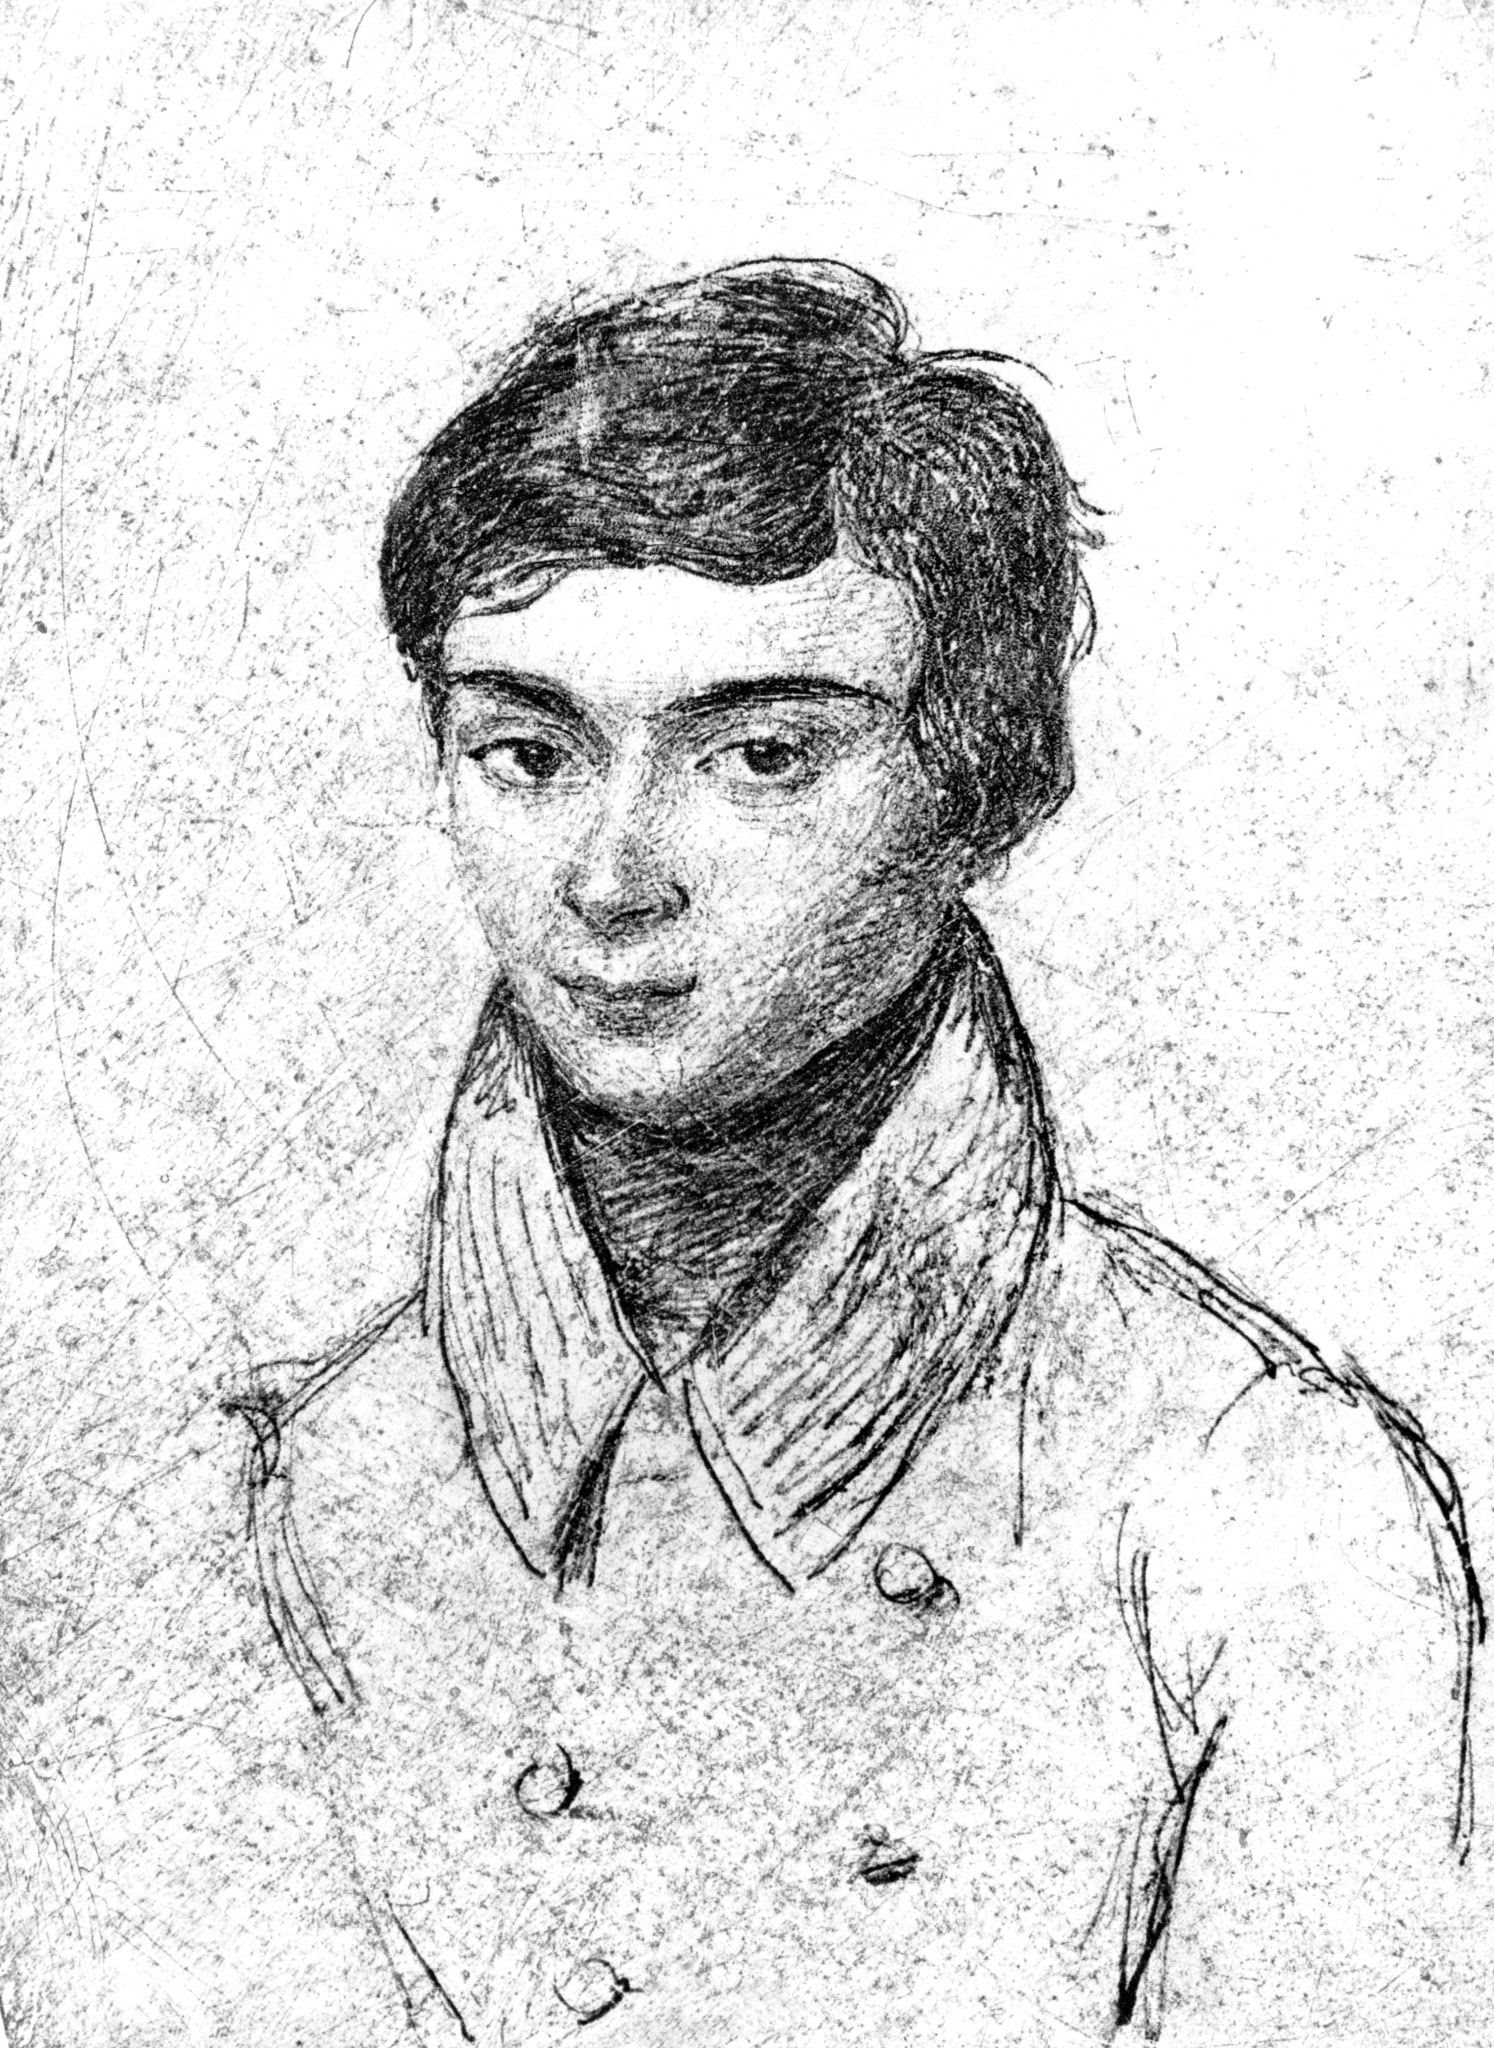
\includegraphics[width= 0.5\linewidth]{20}
%		\caption{\small\textit{\color{toanhocdoisong}Evariste Galois $(1811 - 1832)$.}}
%		\vspace*{-10pt}
%	\end{figure}
	Trong mã Reed -- Solomon, việc mã hóa được tiến hành cho từng gói gồm $k$ phần tử của $GF(2^n)$. Nói cách khác, quá trình mã hóa được tiến hành cùng lúc cho $k$ số nhị phân, mỗi số $n$ bit. Ký hiệu các phần tử của gói là $m_0,m_1,\ldots,m_{k-1}$. Ta xây dựng được một đa thức:
	\begin{align*}
		P(x)=m_0+m_1x+ \cdots +m_{k-1} x^{k-1}.
	\end{align*}
	Chú ý rằng đa thức này khác với những đa thức đã nói ở trên. Những đa thức ở phía trên có hệ số là $0$ hoặc $1$ (phần tử của $GF(2)$) còn đa thức $P(x)$ của ta có các hệ số $m_i$ là các phần tử của $GF(2^n)$. Một từ mã được tạo ra bằng cách tính các giá trị của $P(x)$ cho từng phần tử của trường Galois $GF(2^n)$:
	\begin{align*}
	c &\!=\! \left(c_0,c_1,c_2,\ldots,c_{q-1}\right) \\[-0.5ex]
	&\!=\!\! \left[\!P(0), P(\!\alpha\!), P(\alpha^2), \ldots, P(\alpha^{q-1}\!)\!\right]\!,q \!=\! 2^n,
	\end{align*}
	Do mỗi phần tử $m_i$ có thể nhận một trong $q=2^n$ giá trị nên có tổng cộng $q^k$ từ mã trong mã Reed -- Solomon. Ứng với mỗi từ mã, ta có một hệ phương trình:
	\begin{align*}
		P(0)=\,&m_0, \\[-0.5ex]
		P(\alpha)=\,&m_0+m_1 \alpha+m_2 \alpha^2+\cdots\\[-0.5ex]
		&+m_{k-1} \alpha^{k-1},
		\end{align*}
		\begin{align*}
		P(\alpha^2 )=\,&m_0+m_1 \alpha^2+m_2 \alpha^4+\cdots\\[-0.5ex]
		&+m_{k-1} \alpha^{2(k-1)},\\[-0.5ex]
		...&\\[-0.5ex]
		P(\alpha^{q-1})=\,&m_0+m_1 \alpha^{q-1}+m_2 \alpha^{2(q-1)} \\[-0.5ex]
		&+\cdots+m_{k-1} \alpha^{(k-1)(q-1)}. 
	\end{align*}
	Chọn bất kỳ $k$ trong số $q$ phương trình trên, ta được một hệ phương trình mà từ đó có thể giải để tìm các $m_i$.
	\vskip 0.05cm
	Trong trường hợp đường truyền bị lỗi, giả sử có $t$ trong số $q$ phương trình bị lỗi (các giá trị $P\left(\alpha^i\right)$ tương ứng bị lỗi). Khi đó, nếu ta thử tất cả các tổ hợp có thể gồm $k$ phương trình từ $q$ phương trình, sẽ có $( \begin{array}{l}
		t + k - 1\\[-0.5ex]
		k
	\end{array})$ hệ phương trình cho kết quả $m_i$ khác với các hệ phương trình còn lại. Do đó, việc sửa lỗi có thể được tiến hành bằng cách lấy kết quả chiếm đa số, với điều kiện là  $( \begin{array}{l}
	t + k - 1\\[-0.5ex]
	k
\end{array}) <( \begin{array}{l}
q - t\\[-0.5ex]
k
\end{array})$. Số lỗi lớn nhất có thể sửa là số nguyên $t$ nhỏ hơn hoặc bằng $\dfrac{1}{2}(q-k+1)$.
\vskip 0.05cm
	Việc thử các tổ hợp hệ phương trình khác nhau theo đề xuất ban đầu của Reed và Solomon là tương đối phức tạp về mặt cài đặt trong thực tế nên sau đó người ta đã đưa ra hai hướng tiếp cận khác để tạo mã Reed -- Solomon, một sử dụng đa thức sinh và một sử dụng biến đổi Fourier trên trường Galois (Wicker, $1994$).
	\vskip 0.05cm
	\textbf{\color{toanhocdoisong}Tài liệu tham khảo}
	\vskip 0.05cm
	[$1$] Aktaş, C. ($2017$). \textit{The evolution and emergence of QR codes}. Cambridge Scholars Publishing.
	\vskip 0.05cm
	[$2$] Reed, I. S., \& Solomon, G. ($1960$). \textit{Polynomial Codes Over Certain Finite Fields}. Journal of the Society for Industrial and Applied Mathematics, $8(2)$, $300-304$. 
	\vskip 0.05cm
	[$3$] Wicker, S. B., \& Bhargava, V. K. ($1994$). \textit{Reed--Solomon codes and their applications}. IEEE.
\end{multicols}
%	\newpage
%
%	\setcounter{figure}{0}
%	\thispagestyle{duongvaotoanhocnone}
\pagestyle{duongvaotoanhoc}
\everymath{\color{duongvaotoanhoc}}
\graphicspath{{../duongvaotoanhoc/pic/}}
%\blfootnote{$^1$\color{duongvaotoanhoc}Theo Quanta Magazine.}
%\blfootnote{$^2$\color{duongvaotoanhoc}Hà Nội.}
\begingroup
\AddToShipoutPicture*{\put(0,616){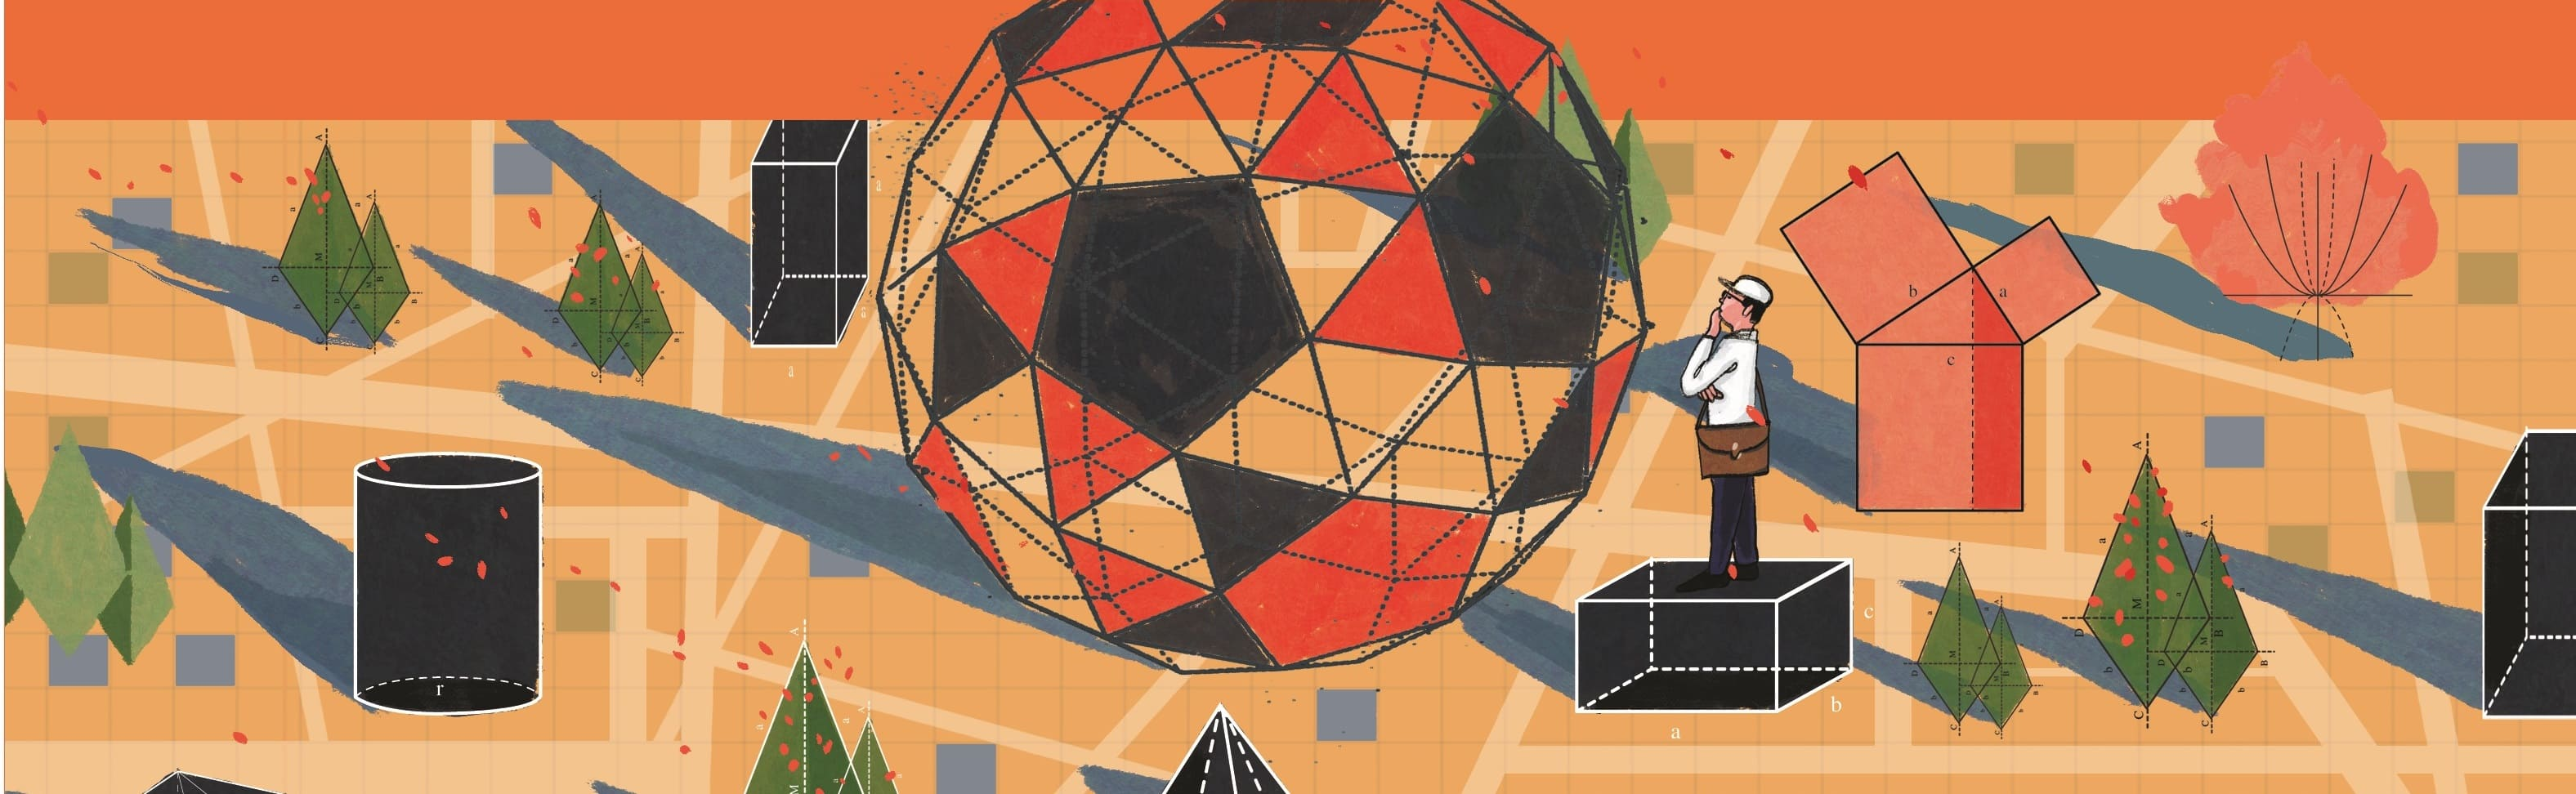
\includegraphics[width=19.3cm]{../bannerduongvao}}}
\AddToShipoutPicture*{\put(82,555){
\includegraphics[scale=1]{../tieude.pdf}}}
\centering
\endgroup

\vspace*{150pt}

\tikzstyle{start} = [rectangle, rounded corners, minimum height=1cm,text centered, draw=black, fill=red!30]

\tikzstyle{end} = [rectangle, rounded corners, minimum height=1cm,text centered, draw=black, fill=blue!30]

\tikzstyle{mid} = [rectangle, rounded corners, minimum height=1cm,text centered, draw=black, fill=green!30]

\begin{multicols}{2}	
	$\pmb{1.}$ \textbf{\color{duongvaotoanhoc}Mở đầu}
	\vskip 0.1cm
	\textbf{\color{duongvaotoanhoc}Từ dải bện...}
	\vskip 0.1cm
	Dải bện đã tồn tại từ nhiều thế kỷ và được sử dụng khắp nơi vì mục đích trang trí cũng như trong đời sống, chẳng hạn trong sản xuất dây thừng hoặc dây cáp. Một dải bện có thể gồm ba sợi, hay cọng, được tết với nhau: cọng trái được vắt qua cọng giữa, rồi đến cọng phải, rồi lại cọng trái, rồi lại cọng phải, cứ thế lặp đi lặp lại (xem Hình $1$). Nhưng ``dải bện" cũng được dùng để chỉ mọi sự đan hay tết của nhiều cọng dây theo một cách nhất định. Trong Hình $2$ và Hình $3$ là một số thí dụ về các dải bện trang trí.
	\begin{figure}[H]
		\vspace*{-5pt}
		\centering
		\captionsetup{labelformat= empty, justification=centering}
		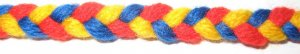
\includegraphics[width= 1\linewidth]{fig_01}
		\caption{\small\textit{\color{duongvaotoanhoc}Hình $1$. Dải bện cổ điển với ba cọng dây.}}
		\vspace*{-10pt}
	\end{figure}
	\begin{figure}[H]
		\vspace*{-5pt}
		\centering
		\captionsetup{labelformat= empty, justification=centering}
		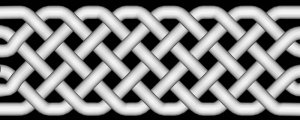
\includegraphics[width= 1\linewidth]{fig_02}
		\caption{\small\textit{\color{duongvaotoanhoc}Hình $2$. Một dải bện trang trí.}}
		\vspace*{-10pt}
	\end{figure}
	\textbf{\color{duongvaotoanhoc}... đến lý thuyết bện}
	\vskip 0.1cm
	Các nhà toán học mô tả các dải bện bằng các mô hình trừu tượng, những đối tượng trung tâm của một lý thuyết toán học có tên ``lý thuyết bện". Lý thuyết này đóng một vai trò trung tâm trong toán học và len lỏi vào trong nhiều ngành toán học, cũng như các khoa học khác như vật lý, sinh học, tin học và mật mã.
	\begin{figure}[H]
		\vspace*{-5pt}
		\centering
		\captionsetup{labelformat= empty, justification=centering}
		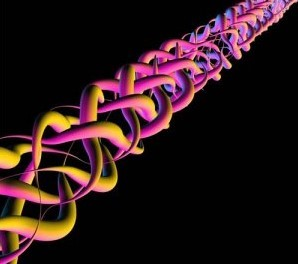
\includegraphics[width= 1\linewidth]{fig_03a}
		\caption{\small\textit{\color{duongvaotoanhoc}Hình $3$. Một dải bện trang trí khác.}}
		\vspace*{-10pt}
	\end{figure}
%	\vskip 0.1cm
	Bài viết này nhằm đem đến cho độc giả không làm toán một cái nhìn bao quát về lý thuyết bện. Chúng tôi sẽ đưa ra định nghĩa bện trong toán học, sau đó minh họa ứng dụng của chúng trong ba lĩnh vực: lý thuyết nút (toán học), lý thuyết thuật toán (toán học và tin học), và lý thuyết mật mã (toán học, tin học và viễn thông). Ngoài ra, chúng còn nhiều ứng dụng và tương tác qua lại khác với các phần khác của toán học, và với cả, chẳng hạn, vật lý thiên văn. Thực vậy, các đường từ trường trong khí quyển Mặt Trời tạo thành các dải bện mà độ phức tạp có liên hệ trực tiếp đến cường độ của từ trường.
	\vskip 0.1cm
	Lý thuyết bện là một lĩnh vực nghiên cứu rất tích cực ở Pháp, được tổ chức xung quanh nhóm nghiên cứu GDR TRESSES. Nhóm nghiên cứu này được thành lập năm $2000$ bởi Patrick Dehornoy với thời gian hoạt động $2$ năm, sau đó được gia hạn $4$ năm, từ $2003$ đến $2007$, dưới sự điều hành của Christian Blanchet (giáo sư tại Đại học Bretagne Sud), và từ năm $2008$ được điều hành bởi Luis Paris (giáo sư tại Đại học Bourgogne). Ngay từ đầu, một đặc thù quan trọng của nhóm nghiên cứu này là hòa trộn các nhà khoa học từ các lĩnh vực khác nhau. Nó gồm $18$ nhóm các nhà toán học và $2$ nhóm các nhà tin học, phân bố khắp nơi trên nước Pháp. Ngoài ra, những buổi họp mặt của nó còn có sự tham dự của nhiều nhà khoa học từ các nước khác. Uy tín quốc tế của GDR TRESSES đã được công nhận: tại hội nghị về lý thuyết bện ở Banff (Canada) vào tháng $4$ năm $2007$, GDR TRESSES được giới thiệu như một mô hình nghiên cứu kiểu mẫu.
	\vskip 0.1cm
	\PIbox{
	\begin{figure}[H]
		\vspace*{-10pt}
		\centering
		\captionsetup{labelformat= empty, justification=centering}
		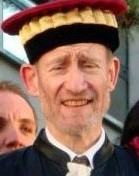
\includegraphics[width= 1\linewidth]{fig_Dehornoy}
		\caption{\small\textit{\color{duongvaotoanhoc}Patrick Dehornoy.}}
		\vspace*{-10pt}
	\end{figure}
	Patrick Dehornoy ($1952-2019$) là nhà toán học Pháp được biết đến vì những công trình trong lý thuyết tập hợp và lý thuyết bện. Ông nguyên là giáo sư tại Đại học Caen và là thành viên kỳ cựu của Viện Đại học Pháp (Institut Universitaire de France). Ông là người sáng lập nhóm nghiên cứu GDR TRESSES, nơi tập trung các nghiên cứu về lý thuyết bện của nước Pháp.
	}
	\vskip 0.1cm
	$\pmb{2.}$ \textbf{\color{duongvaotoanhoc}Dải bện trong toán học}
	\vskip 0.1cm
	\textbf{\color{duongvaotoanhoc}Thế nào là một dải bện trong toán học?}
	\vskip 0.1cm
	\textit{Lý thuyết bện} tách khái niệm bện khỏi những dải bện mà ta vẫn thường nghĩ đến. Trước tiên, ta cố định một số tự nhiên $n$. Để tiện trình bày, ta sẽ lấy $n = 4$, mặc dù tất cả những gì được mô tả tiếp theo đây đúng với mọi giá trị của $n$. Chúng ta lấy hai tập hợp, mỗi tập hợp có $4$ vật (chẳng hạn những cái đinh) và để chúng trên bàn thành hai hàng dọc đối diện nhau (các chấm đen trong hình). Sử dụng bốn sợi dây, mà ta gọi là cọng, ta nối mỗi vật trong tập hợp thứ nhất với một vật trong tập hợp thứ hai. Một kết nối như vậy được gọi là một dải bện. Các cọng có thể vắt qua nhau, nhưng không được vòng ngược lại. Kết nối trong Hình $5$ không phải là một dải bện (theo nghĩa toán học).
	\begin{figure}[H]
		\vspace*{-5pt}
		\centering
		\captionsetup{labelformat= empty, justification=centering}
		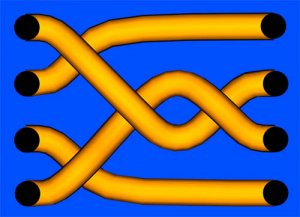
\includegraphics[width= 0.48\linewidth]{fig_04}
		\caption{\small\textit{\color{duongvaotoanhoc}Hình $4$. Một dải bện toán học.}}
		\vspace*{-10pt}
	\end{figure}
	\begin{figure}[H]
		\vspace*{-10pt}
		\centering
		\captionsetup{labelformat= empty, justification=centering}
		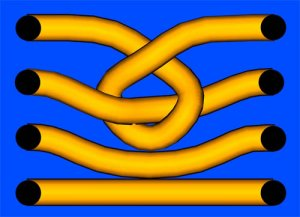
\includegraphics[width= 0.48\linewidth]{fig_05}
		\caption{\small\textit{\color{duongvaotoanhoc}Hình $5$. Đây không phải một dải bện.}}
		\vspace*{-10pt}
	\end{figure}	
	Trong Hình $6$ là hai dải bện khác nhau. Trong khi đó, hai dải bện trong Hình $7$ là giống nhau, vì chúng có thể nhận được từ nhau bằng cách ``xê dịch" các cọng.
	\begin{figure}[H]
		\vspace*{-5pt}
		\centering
		\captionsetup{labelformat= empty, justification=centering}
		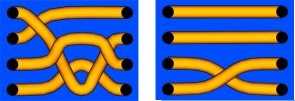
\includegraphics[width= 1\linewidth]{fig_06}
		\caption{\small\textit{\color{duongvaotoanhoc}Hình $6$. Hai dải bện khác nhau.}}
		\vspace*{-5pt}
	\end{figure}
	\begin{figure}[H]
		\vspace*{2pt}
		\centering
		\captionsetup{labelformat= empty, justification=centering}
		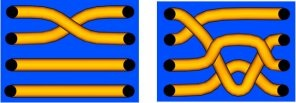
\includegraphics[width= 0.97\linewidth]{fig_07}
		\caption{\small\textit{\color{duongvaotoanhoc}Hình $7$. Hai dải bện giống nhau.}}
		\vspace*{-10pt}
	\end{figure}
	Một dải bện cũng có thể được coi như một chuỗi các đường đi của $4$ hạt không gặp nhau. Ở đây, tập hợp các điểm xuất phát trùng với tập hợp các điểm đến. Thí dụ, các quỹ đạo của $4$ hạt được thể hiện ở nửa trên của Hình $8$ tương ứng với dải bện ở nửa dưới. Một cách nôm na, các dải bện có thể được xem như những điệu nhảy mà ở đó, mỗi vũ công kết thúc ở vị trí của một vũ công khác.
	\begin{figure}[H]
		\vspace*{-5pt}
		\centering
		\captionsetup{labelformat= empty, justification=centering}
		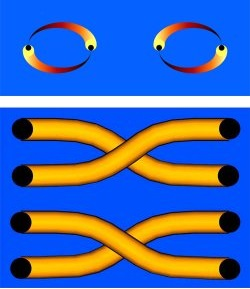
\includegraphics[width= 0.475\linewidth]{fig_08}
		\caption{\small\textit{\color{duongvaotoanhoc}Hình $8$. Hai cách nhìn của cùng một dải bện.}}
		\vspace*{-10pt}
	\end{figure}
	\textbf{\color{duongvaotoanhoc}Ghép các dải bện}
	\vskip 0.05cm
	Từ hai dải bện $\alpha$ và $\beta$, ta có thể xây dựng một phép thứ ba, ký hiệu là $\alpha \beta$ và được gọi là dải bện hợp thành của $\alpha$ và $\beta$, bằng cách ghép chúng với nhau. Trong Hình $9$ là hai dải bện (bên trên) và hợp thành của chúng (bên dưới).
	\begin{figure}[H]
		\vspace*{-5pt}
		\centering
		\captionsetup{labelformat= empty, justification=centering}
		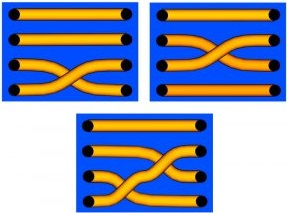
\includegraphics[width= 0.97\linewidth]{fig_09}
		\caption{\small\textit{\color{duongvaotoanhoc}Hình $9$. Hợp thành của hai dải bện.}}
		\vspace*{-5pt}
	\end{figure}
	Một thí dụ khác về phép hợp thành được minh họa trong Hình $10$.
	\begin{figure}[H]
		\vspace*{-5pt}
		\centering
		\captionsetup{labelformat= empty, justification=centering}
		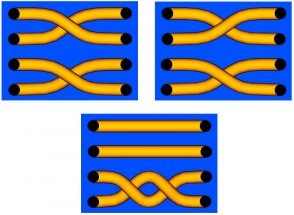
\includegraphics[width= 0.97\linewidth]{fig_10}
		\caption{\small\textit{\color{duongvaotoanhoc}Hình $10$. Hợp thành của hai dải bện khác.}}
		\vspace*{-10pt}
	\end{figure}
	Bạn đọc có kinh nghiệm hẳn đã để ý rằng dải bện $\alpha \beta$ có thể khác với dải bện $\beta \alpha$: điều này xảy ra với thí dụ trong Hình $9$, nhưng không đúng với thí dụ trong Hình $10$.
	\vskip 0.1cm
	Dải bện trong Hình $11$ được gọi là \textit{dải bện tầm thường}. Dễ thấy hợp của một dải bện $\alpha$ bất kỳ với dải bện tầm thường, từ bên trái hay từ bên phải, vẫn là $\alpha$.
	\begin{figure}[H]
		\vspace*{-5pt}
		\centering
		\captionsetup{labelformat= empty, justification=centering}
		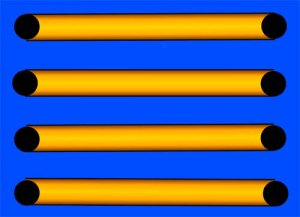
\includegraphics[width= 0.47\linewidth]{fig_11}
		\caption{\small\textit{\color{duongvaotoanhoc}Hình $11$. Dải bện tầm thường.}}
		\vspace*{-10pt}
	\end{figure}
	Nếu ta đặt một tấm gương vuông góc với mặt bàn ở cạnh hàng đinh thứ hai, ảnh phản chiếu trong gương của dải bện $\alpha$ được gọi là dải bện đối xứng của $\alpha$ (xem Hình $12$). Hợp thành của một dải bện với dải bện đối xứng của nó là dải bện tầm thường. Bạn đọc có thể dễ dàng kiểm chứng với thí dụ trong Hình $12$.
	\begin{figure}[H]
		\vspace*{-5pt}
		\centering
		\captionsetup{labelformat= empty, justification=centering}
		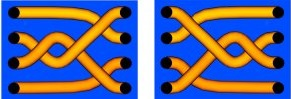
\includegraphics[width= 0.97\linewidth]{fig_12}
		\caption{\small\textit{\color{duongvaotoanhoc}Hình $12$. Một dải bện và dải bện đối xứng của~nó.}}
		\vspace*{-5pt}
	\end{figure}
	\textbf{\color{duongvaotoanhoc}Từ dải bện đến nhóm bện}
	\vskip 0.1cm
	Những dải bện, như chúng ta vừa định nghĩa, cùng với phép hợp thành tạo thành cái mà các nhà toán học gọi là \textit{nhóm bện}. Chúng ta có một nhóm bện [gồm các dải bện có] hai cọng, một nhóm bện ba cọng, v.v. Nhóm bện một cọng chỉ gồm dải bện tầm thường, vì một cọng thì không thể được bện, dù nó có thể được buộc thắt nút (xem Hình $13$).
	\begin{figure}[H]
		\vspace*{-5pt}
		\centering
		\captionsetup{labelformat= empty, justification=centering}
		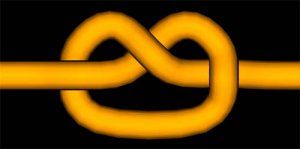
\includegraphics[width= 0.6\linewidth]{fig_13}
		\caption{\small\textit{\color{duongvaotoanhoc}Hình $13$. Cọng buộc thắt nút.}}
		\vspace*{-10pt}
	\end{figure}
	Phép hợp thành của các dải bện tuân theo một số quy tắc mà đối với các nhà toán học cũng quan trọng không kém, nếu không nói là hơn, chính các dải bện.
	Nguồn gốc của lý thuyết bện
	\vskip 0.1cm
	Nghiên cứu toán học về các dải bện thường được cho là bắt đầu từ bài báo năm $1925$ của Emil Artin [$4$], trong đó ông mô tả khái niệm dải bện dưới nhiều khía cạnh khác nhau, cái thì hiển nhiên như ``một chuỗi các cọng dây được kéo căng và quấn vào nhau", những cái khác toán học hơn, chẳng hạn như nhóm được cho bởi ``các phần tử sinh và các quan hệ", hay như ``nhóm các tự đẳng cấu của một nhóm tự do", hay như  ``nhóm các phép đẳng luân của một đĩa bị thủng". Chính sự đa dạng của các cách tiếp cận khác nhau này tạo nên tính hấp dẫn của các nhóm bện.
	\vskip 0.15cm
	\PIbox{
	Emil Artin ($1898-1962$) là nhà toán học người Áo. Ông làm việc ở Đức (chủ yếu ở Hamburg) đến năm $1937$. Ông sang Mỹ và làm giáo sư tại Đại học Indiana từ năm $1938$ đến năm $1946$, rồi tại Đại học Princeton từ năm $1946$ đến năm $1958$. Ông là một trong những nhà đại số xuất sắc nhất thế kỷ $20$. Đặc biệt, ông là người khai sinh lý thuyết bện.
	}
	\vskip 0.1cm
	\begin{figure}[H]
		\vspace*{2pt}
		\centering
		\captionsetup{labelformat= empty, justification=centering}
		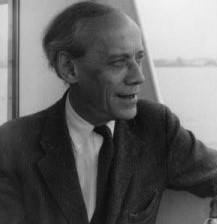
\includegraphics[width= 0.47\linewidth]{fig_Artin}
		\caption{\small\textit{\color{duongvaotoanhoc}Emil Artin}}
		\vspace*{-10pt}
	\end{figure}
	$\pmb{3.}$ \textbf{\color{duongvaotoanhoc}Từ dải bện đến lý thuyết nút}
	\vskip 0.1cm
	\textbf{\color{duongvaotoanhoc}Nút trong toán học là gì?}
	\vskip 0.1cm
	Một \textit{nút} trong toán học là một vòng dây khép kín (không có hai đầu, xem Hình $14$). Một \textit{cuộn dây gồm hai thành phần} được tạo bởi hai vòng dây khép kín (xem Hình $15$), một \textit{cuộn dây gồm ba thành phần} được tạo bởi ba vòng dây khép kín, v.v. \textit{Lý thuyết nút} là nhánh của tô--pô nghiên cứu các nút và các cuộn. Trong tô--pô, hình cầu không phân biệt với hình lập phương, còn cái bánh vòng và tách trà là một. Người ta không xét đến các thuộc tính như độ dài hay góc, mục đích là hiểu các tính chất bất biến đối với sự xoắn, kéo dãn hay nén.
	\begin{figure}[H]
		\vspace*{-10pt}
		\centering
		\captionsetup{labelformat= empty, justification=centering}
		
\includegraphics[width= 0.47\linewidth]{fig_14}
		\caption{\small\textit{\color{duongvaotoanhoc}Hình $14$. Một nút.}}
		\vspace*{-10pt}
	\end{figure}
	\begin{figure}[H]
		\vspace*{-10pt}
		\centering
		\captionsetup{labelformat= empty, justification=centering}
		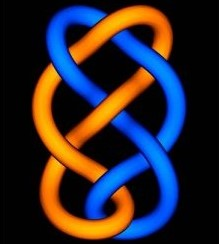
\includegraphics[width= 0.47\linewidth]{fig_15}
		\caption{\small\textit{\color{duongvaotoanhoc}Hình $15$. Một cuộn dây gồm hai thành phần.}}
		\vspace*{-10pt}
	\end{figure}
	Ngoài toán học, đặc biệt là tô--pô, lý thuyết nút có những ứng dụng trong các bài toán sinh học và hóa học. Chẳng hạn, nó được dùng trong nghiên cứu các phân tử đồng phân (có cùng công thức hóa học nhưng được sắp xếp khác nhau) hoặc trong nghiên cứu về tác động của một số enzyme đối với ADN.
	\vskip 0.1cm
	\textbf{\color{duongvaotoanhoc}Nguồn gốc của lý thuyết nút}
	\vskip 0.1cm
	Đóng góp đáng kể đầu tiên vào lý thuyết nút có lẽ là của Sir William Thomson (tức Kelvin) với thuyết ``xoáy nguyên tử" của ông. Năm $1867$, sau khi quan sát các vòng khói được tạo ra từ thí nghiệm của Peter Tait, nhà vật lý người Scotland, Thomson kết luận rằng các nguyên tử là những nút của ``những cuộn xoáy trong ê--te truyền ánh sáng". Theo đó, các nguyên tố hóa học ứng với các nút hoặc cuộn dây. Từ ý tưởng này, Peter Tait bắt đầu phân loại các nút, với niềm tin rằng ông đang tạo ra một bảng nguyên tố hóa học.
	\vskip 0.15cm
	\PIbox{
	\begin{figure}[H]
		\vspace*{-15pt}
		\centering
		\captionsetup{labelformat= empty, justification=centering}
		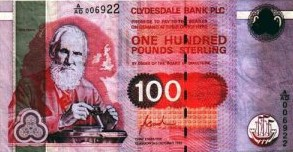
\includegraphics[width= 1\linewidth]{fig_William}
		\caption{\small\textit{\color{duongvaotoanhoc}William Thomson.}}
		\vspace*{-10pt}
	\end{figure}
	Sir William Thomson ($1824-1907$) là nhà vật lý học, nhà toán học và kỹ sư người Scotland. Ông được coi là một trong những nhà vật lý học hàng đầu của thế kỷ~$19$.
	}
	\vskip 0.1cm
	\textbf{\color{duongvaotoanhoc}Bài toán phân biệt hai nút}
	\vskip 0.1cm
	Bài toán trung tâm của lý thuyết nút là phân biệt, và xa hơn là phân loại, các nút. Phân biệt có nghĩa là quyết định xem liệu hai hình vẽ nút (hoặc cuộn dây) có biểu diễn cùng một nút (hoặc cuộn dây) hay không. Trong những năm $1920$, hai nhà toán học Mỹ Alexander và Briggs [$2$] và nhà toán học Đức Reidemeister [$16$], độc lập với nhau, đề xuất một thuật toán giải quyết một phần bài toán này. Thuật toán này có thể trả lời khẳng định nếu hai hình vẽ biểu diễn cùng một nút (hoặc cuộn), nhưng nó không trả lời trong trường hợp ngược lại. Nói cách khác, ta có thể nói hai nút giống nhau hay không, nhưng không thể nói hai nút có khác nhau hay không. Độc giả có thể cảm thấy điều này thật vô lý, nhưng nó là một nghịch lý thường thấy trong toán học. Hãy tưởng tượng bạn đang chờ ai đó. Bạn tự nhủ: ``Nếu cậu ấy đến, đó đúng là một người bạn." Nhưng nếu người đó không đến, bạn sẽ không biết đó có phải một người bạn hay không.
	\vskip 0.05cm
	Để phân biệt các nút, người ta sử dụng những cái mà các nhà toán học gọi là những \textit{bất biến}. Người ta gán cho mỗi hình vẽ cái nút một đối tượng (thường là một số hoặc một đa thức) chỉ phụ thuộc vào cái nút mà không phụ thuộc vào cách nó được vẽ. Nếu hai nút có những bất biến khác nhau thì chúng là hai nút khác nhau. Nếu không, ta chưa thể kết luận được gì.
	\vskip 0.1cm
	\textbf{\color{duongvaotoanhoc}Từ dải bện đến nút}
	\begin{figure}[H]
		\vspace*{-10pt}
		\centering
		\captionsetup{labelformat= empty, justification=centering}
		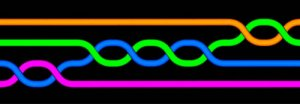
\includegraphics[width= 1\linewidth]{fig_16}
		\caption{\small\textit{\color{duongvaotoanhoc}Hình $16$. Dải bện đóng.}}
		\vspace*{-10pt}
	\end{figure}
	Từ một dải bện, ta có thể tạo ra một cuộn dây (hoặc một nút) bằng cách nối các đầu của dải bện với nhau, như minh họa trong Hình $16$. Một cuộn dây như vậy được gọi là một dải bện đóng. Alexander [$1$] đã chứng minh rằng mọi cuộn dây đều có thể được tạo ra theo cách này. Bạn đọc có thể thử với các thí dụ trong Hình $14$ và Hình $15$. Sau đó, Markov [$15$] đưa ra một thuật toán không hoàn toàn để xác định liệu hai dải bện cho trước có tạo thành cùng một cuộn dây (nhưng nó có thể không trả lời). Đây là hai kết quả cốt yếu để áp dụng lý thuyết bện vào các nút. Đặc biệt, chúng là điểm bắt đầu của sự đổi mới sâu sắc trong lý thuyết nút trong thập niên $1980$,
%	với những công trình của Jones [$12$, $13$] và những bất biến được định nghĩa từ lý thuyết bện.
%	\vskip 0.01cm
%	\begin{tBox}
%		\begin{wrapfigure}{l}{0.45\linewidth}
%			\vspace*{-15pt}
%			\centering
%			\captionsetup{labelformat= empty, justification=centering}
%			\hspace*{2pt}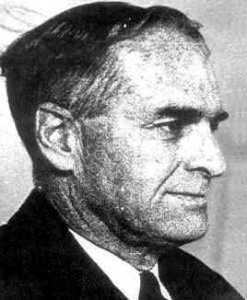
\includegraphics[width= 1.1\linewidth]{fig_Alexander}
%			\caption{\small\textit{\color{duongvaotoanhoc}Alexander.}}
%			\vspace*{-10pt}
%		\end{wrapfigure}
%		James W. Alexander ($1888-1971$) là một nhà toán học nổi tiếng người Mỹ. Là một trong những thành viên đầu tiên của Viện Nghiên cứu Cao cấp Princeton (từ $1933$ đến $1951$), ông đồng thời là giáo sư tại Đại học Princeton (từ $1920$ đến $1951$). Ông là một trong những người tiên phong của tô--pô đại số và lý thuyết nút. Ông cũng là một nhà leo núi cừ khôi, từng chinh phục được nhiều đỉnh cao. Về cuối đời, ông trở nên đơn độc và ẩn dật. Ông được biết đến như một người theo chủ nghĩa xã hội tích cực và danh tiếng của ông khiến ông bị chủ nghĩa MacCarthy để ý. Ông không xuất hiện trước công chúng kể từ năm $1954$, sau khi ký tên vào một bức thư ủng hộ Robert Oppenheimer.
%	\end{tBox}
%
%	\vspace*{-8pt}
%	\begin{tBox}
%		\begin{wrapfigure}{r}{0.4\linewidth}
%			\vspace*{-15pt}
%			\centering
%			\captionsetup{labelformat= empty, justification=centering}
%			\hspace*{-10pt}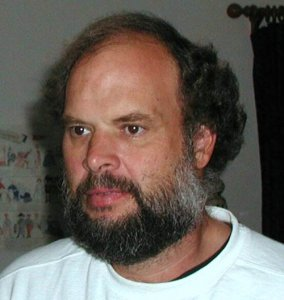
\includegraphics[width= 1.1\linewidth]{fig_Jones}
%			\caption{\small\textit{\color{duongvaotoanhoc}Jones.}}
%			\vspace*{-15pt}
%		\end{wrapfigure}
%		Vaughan F.R. Jones ($1952-2020$) là nhà toán học người New Zealand nổi tiếng với những công trình về các đại số von Neumann, các bất biến nút và lý thuyết trường bảo giác. Ông được trao Huy chương Fields năm $1990$ và là giáo sư ($1985-2011$) rồi giáo sư danh dự ($2011$ đến khi mất) tại Đại học California tại Berkeley. Các công trình của ông về bất biến nút dẫn tới những lời giải bất ngờ cho nhiều bài toán cổ điển trong lý thuyết nút và tô--pô thấp chiều.
%	\end{tBox}
%	\vskip 0.05cm
%	\textbf{\color{duongvaotoanhoc}Phân biệt hai dải bện}
%	\vskip 0.1cm
%	Khác với nút, với dải bện tồn tại các thuật toán để xác định xem hai dải bện có giống nhau hay không. Nhiều thuật toán trong số này rất nhanh và đã được đưa vào các phần mềm tính toán như GAP hay MAGMA. Sự tồn tại của các thuật toán này liên quan đến việc các dải bện không chỉ là những đối tượng tô--pô, mà còn là những \textit{đối tượng đại số}, bởi như đã thấy, ta có thể áp dụng phép hợp thành lên chúng. Dưới đây là một cách xác định liệu hai dải bện có bằng nhau hay không. Rất có thể quá trình này đã được Artin biết đến từ năm $1925$.
%	\vskip 0.1cm
%	Xét hai (hình) dải bện $\alpha$ và $\beta$.
%	\vskip 0.1cm
%	Bước $1$: Gọi $\tilde \beta$ là dải bện đối xứng của $\beta$. Để ý rằng $\alpha$ và $\beta$ là cùng một dải bện nếu và chỉ nếu dải bện hợp thành $\alpha \tilde \beta$ là tầm thường. Đặt $\gamma = \alpha \tilde \beta$. Bài toán trở thành xác định xem $\gamma$ có phải dải bện tầm thường hay không.
%	\vskip 0.1cm
%	Bước $2$: Để $\gamma$ là dải bện tầm thường thì cọng đi từ đinh trên cùng bên trái phải nối đến đinh trên cùng bên phải, cọng từ đinh thứ hai bên trái nối đến đinh thứ hai bên phải, v.v. Ta kiểm tra điều này với $\gamma$. Nếu $\gamma$ không thỏa mãn thì nó không tầm thường. Thí dụ, dải bện trong Hình $17$ không tầm thường vì cọng đi từ đinh dưới cùng bên trái nối đến đinh thứ hai từ trên xuống ở bên phải. Còn nếu $\gamma$ thỏa mãn, ta chuyển sang bước $3$.
%	\begin{figure}[H]
%		\vspace*{-5pt}
%		\centering
%		\captionsetup{labelformat= empty, justification=centering}
%		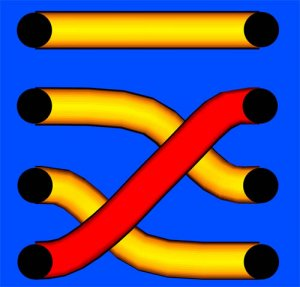
\includegraphics[width= 0.48\linewidth]{fig_17}
%		\caption{\small\textit{\color{duongvaotoanhoc}Hình $17$. Một dải bện không tầm thường.}}
%		\vspace*{-10pt}
%	\end{figure}
%	Bước $3$: Nếu bỏ đi cọng dây trên cùng, ta nhận được một dải bện $\gamma'$ gồm $3$ cọng (có thể làm điều này vì cọng dây nối đinh trên cùng bên trái với đinh trên cùng bên phải). Giả sử ta đã biết cách phân biệt hai dải bện gồm $3$ cọng. Để $\gamma$ là tầm thường thì $\gamma'$ cũng phải tầm thường. Thí dụ, dải bện $\gamma$ trong Hình $18$ không tầm thường vì $\gamma'$ không tầm thường. Nếu $\gamma'$ là tầm thường, ta chuyển sang bước~$4$.
%	\begin{figure}[H]
%		\vspace*{-5pt}
%		\centering
%		\captionsetup{labelformat= empty, justification=centering}
%		\includegraphics[width= 0.48\linewidth]{fig_18}
%		\caption{\small\textit{\color{duongvaotoanhoc}Hình $18$. Xóa một cọng dây.}}
%		\vspace*{-10pt}
%	\end{figure}
%	Bước $4$: Tới bước này, ba cọng bên dưới của dải bện của chúng ta là các đoạn thẳng, trong khi cọng bị xóa vắt qua chúng, như minh họa trong Hình $19$. Tới đây cần những công cụ toán học phức tạp hơn, nhưng bạn đọc có thể nắm được rằng người ta biết cách xử lý trường hợp này một cách không quá khó khăn, nhưng cần những công cụ mà trong khuôn khổ bài viết này không đủ chỗ để giải thích.
%	\begin{figure}[H]
%		\vspace*{-5pt}
%		\centering
%		\captionsetup{labelformat= empty, justification=centering}
%		\includegraphics[width= 0.48\linewidth]{fig_19}
%		\caption{\small\textit{\color{duongvaotoanhoc}Hình $19$. Một cọng vắt qua các cọng khác.}}
%		\vspace*{-10pt}
%	\end{figure}
%	$\pmb{4.}$ \textbf{\color{duongvaotoanhoc}Từ dải bện đến thuật toán}
%	\vskip 0.1cm
%	\textbf{\color{duongvaotoanhoc}Thuật toán và ngôn ngữ}
%	\vskip 0.1cm
%	Nếu bạn chỉ đường cho một người khách đến chơi nhà mình, bạn đang tạo ra (và cho thực hiện) một thuật toán đấy! Một \textit{thuật toán} là một dãy các chỉ dẫn (toán học hoặc không) được định nghĩa rõ ràng nhằm thực hiện một công việc nào đó. Nếu thuật toán đúng, kết quả nhận được sẽ là kết quả mong muốn và vị khách sẽ tìm được đường đến đúng nhà bạn. Nếu thuật toán sai, kết quả có thể ngoài dự kiến. Trong tin học, thuật toán cho phương pháp, và việc lập trình chuyển nó thành dạng các câu lệnh cho máy tính.
%	\vskip 0.1cm
%	Một khái niệm quan trọng trong khoa học thuật toán là từ và ngôn ngữ. Với một nhà nghiên cứu thuật toán, một \textit{bảng chữ cái} là một tập hợp hữu hạn mà các phần tử được gọi là các chữ cái, một từ là một dãy hữu hạn các chữ cái, và một \textit{ngôn ngữ} là một tập hợp các từ. Thí dụ, tập hợp $\mathcal A = \{a, b\}$ là một bảng chữ cái, các dãy $b, ab, aab, aaab$ là các từ, và tập hợp $\{b, ab, aab, aaab, aaaab, \dots\}$ là một ngôn ngữ. Một thí dụ khác: ADN là thuật toán nền tảng để xây dựng nên sự sống. Mỗi phân tử ADN là một chuỗi được tạo thành từ bốn phần tử: adenine (A), thymine (T), cytosine (C) và guanine (G). Số phần tử cũng như thứ tự sắp xếp của chúng sẽ quyết định tạo ra con muỗi hay con sư tử. Một cách ngắn gọn: mỗi từ tạo thành từ bảng chữ cái $\{A, T, C, G\}$ biểu diễn một thuật toán để tạo ra một sinh vật, và tập hợp tất cả các sinh vật có thể được xem như một ngôn ngữ trên bảng chữ cái $\{A, T, C, G\}$. Đó là khởi đầu việc mô hình hóa trong di truyền học.
%	\vskip 0.1cm
%	\textbf{\color{duongvaotoanhoc}Từ dải bện đến các từ}
%	\vskip 0.1cm
%	Chúng ta có thể biểu diễn các dải bện bằng các từ mà không cần đến hình vẽ. Bảng chữ cái được dùng ở đây là $\mathcal A = \{a, b, c, A, B, C\}$. Mỗi chữ cái trong bảng chữ cái này tương ứng với một dải bện ``sơ cấp", xem Hình $20$. Cho một dải bện $\alpha$ bất kỳ, bằng cách cắt $\alpha$ thành các lát nhỏ theo chiều dọc, ta có thể dễ dàng nhận thấy rằng $\alpha$ là hợp thành của nhiều dải bện sơ cấp. Nói cách khác, $\alpha$ có thể được viết như một từ trên bảng chữ cái $\mathcal A$. Thí dụ, dải bện trong Hình $21$ tương ứng với từ $aabC$.
%	\begin{figure}[H]
%		\vspace*{-5pt}
%		\centering
%		\captionsetup{labelformat= empty, justification=centering}
%		\includegraphics[width= 0.65\linewidth]{fig_20}
%		\caption{\small\textit{\color{duongvaotoanhoc}Hình $20$. Dải bện sơ cấp.}}
%%		\vspace*{-5pt}
%	\end{figure}
%	\begin{figure}[H]
%		\vspace*{5pt}
%		\centering
%		\captionsetup{labelformat= empty, justification=centering}
%		\includegraphics[width= 0.48\linewidth]{fig_21}
%		\caption{\small\textit{\color{duongvaotoanhoc}Hình $21$. Dải bện $aabC$.}}
%		\vspace*{-10pt}
%	\end{figure}
%	Nhóm bện được đặc trưng bởi hai tính chất sau:
%	\vskip 0.1cm
%	$1$. Mọi dải bện đều viết được dưới dạng một từ trên bảng chữ cái $\mathcal A = \{a, b, c, A, B, C\}$;
%	\vskip 0.1cm
%	$2$. Ta có các đẳng thức sau:
%	\begin{align*}
%		&aA = Aa = \varepsilon\,, bB = Bb = \varepsilon\,, cC = Cc = \varepsilon\,\\
%		&aba = bab\,, ac = ca\,, bcb = cbc\,,
%	\end{align*}
%	ở đó $\varepsilon$ chỉ từ rỗng, tức là từ có độ dài $0$, không có chữ cái nào. Đẳng thức $aba = bab$ được minh họa trong Hình $22$.
%	\begin{figure}[H]
%		\vspace*{-5pt}
%		\centering
%		\captionsetup{labelformat= empty, justification=centering}
%		\includegraphics[width= 1\linewidth]{fig_22}
%		\caption{\small\textit{\color{duongvaotoanhoc}Hình $22$. Đẳng thức $aba = bab$.}}
%		\vspace*{-10pt}
%	\end{figure}
%	\textbf{\color{duongvaotoanhoc}Bài toán từ và bài toán liên hợp}
%	\vskip 0.1cm
%	Tồn tại một thuật toán nhận đầu vào là hai từ trên bảng chữ cái $\mathcal A = \{a, b, c, A, B, C\}$ và quyết định liệu chúng có biểu diễn cùng một dải bện hay không. Một thuật toán như vậy được gọi là một lời giải cho \textit{bài toán từ}. Bạn đọc có lẽ cũng đã để ý rằng bài toán này rõ ràng chính là một bài toán đã được nói đến ở bên trên: xác định xem hai hình vẽ có biểu diễn cùng một dải bện hay không.
%	\vskip 0.1cm
%	Và đây là một bài toán nữa về dải bện mà chúng ta có thuật toán để giải. Cho hai dải bện $\alpha$ và $\beta$, chúng ta có thể trả lời rằng có hay không một dải bện $\gamma$ sao cho $\alpha \gamma = \gamma \beta$, và trong trường hợp câu trả lời là khẳng định, ta còn biết cách tìm tất cả các $\gamma$ thỏa mãn. Độc giả có thể nhận ra rằng bài toán này chính là giải phương trình $\alpha X = X \beta$. Nhắc lại rằng giải phương trình $\alpha X = X \beta$ nghĩa là tìm tập hợp tất cả các $X$ thỏa mãn đẳng thức này. Nếu không tồn tại $X$ như vậy, tập hợp này là rỗng. Một thuật toán giải phương trình $\alpha X = X \beta$ với $\alpha$ và $\beta$ cho trước được gọi là một lời giải cho \textit{bài toán liên hợp}.
%	\vskip 0.1cm
%	\textbf{\color{duongvaotoanhoc}Bài toán quyết định}
%	\vskip 0.1cm
%	Bài toán từ và bài toán liên hợp thuộc vào họ các bài toán trong toán học, rất gần với thuật toán và tin học, được gọi là ``các bài toán quyết định". Các bài toán quyết định nhận được sự quan tâm ngày càng tăng không chỉ vì ứng dụng của chúng trong nhiều lĩnh vực khác, mà còn vì chính những thay đổi của khái niệm chứng minh toán học. Quả vậy, ngày nay người ta phân biệt khái niệm chứng minh và khái niệm chứng minh ``thực sự", tức là phải xây dựng được lời giải. Một xây dựng như vậy được thực hiện bởi một thuật toán và độ phức tạp (tức thời gian tính toán) của nó là một dữ liệu cần được tính toán và được quan tâm bởi những kỹ sư tin học muốn sử dụng nó.
%	\vskip 0.1cm
%	\textbf{\color{duongvaotoanhoc}Kết quả toán học không xây dựng bằng thuật toán}
%	\vskip 0.1cm
%	Định lý sau đây là một thí dụ về một chứng minh không xây dựng. Nó thường được biết đến dưới cái tên \textit{định lý bánh mỳ kẹp} (xem Hình $23$).
%	\begin{figure}[H]
%		\vspace*{-5pt}
%		\centering
%		\captionsetup{labelformat= empty, justification=centering}
%		\includegraphics[width= 0.9\linewidth]{fig_23}
%		\caption{\small\textit{\color{duongvaotoanhoc}Hình $23$. Định lý bánh mỳ kẹp không áp dụng được trong thực tế.}}
%		\vspace*{-5pt}
%	\end{figure}
%	\textbf{\color{duongvaotoanhoc}Định lý:} Với mọi cái bánh mỳ kẹp gồm bánh mỳ, giăm--bông và phô--mai, luôn tồn tại một nhát cắt đều, tức là sao cho hai phần nhận được có lượng bánh mỳ, giăm bông và phô--mai bằng nhau.
%	\vskip 0.1cm
%	Dù biết là một nhát cắt như thế tồn tại, ta không biết cách nào tìm ra nó. Tuy nhiên, không như vẻ bề ngoài của nó, lý thuyết dẫn đến định lý này không hề vô dụng một chút nào (hình ảnh bánh mỳ kẹp chỉ là minh họa dễ hiểu). Chẳng hạn, với chính những kỹ thuật đó, các nhà toán học đã thiết lập được sự tồn tại của những enzyme có tên topoisomerase có khả năng làm biến đổi hình dạng của ADN.
%	\vskip 0.1cm
%	\textbf{\color{duongvaotoanhoc}Các bài toán quyết định về dải bện}
%	\vskip 0.1cm
%	Thuật toán trong các nhóm bện được nghiên cứu đặc biệt tích cực. Nhiều bài toán quyết định như bài toán từ hay bài toán liên hợp, được Garside [$11$] giải quyết vào năm $1969$. Không có thêm nhiều đột phá, cho đến khi cuốn sách của Epstein et al. được xuất bản. Cuốn sách này mô tả nhiều thuật toán bắt nguồn từ lý thuyết ô--tô--mát để giải các bài toán quyết định trong nhóm bện.
%	\vskip 0.1cm
%	Frank A. Garside đang là giám đốc một trường nam sinh khi ông bắt đầu làm nghiên cứu sinh tiến sỹ tại Oxford vào năm $1968$. Với một công việc toàn thời gian, ông biết rằng tốc độ làm việc của mình sẽ chậm và lựa chọn một chủ đề xa với những xu hướng chủ đạo đương thời: ông tìm cách giải bài toán liên hợp trong nhóm bện. Ông phát hiện ra một cấu trúc khi đó còn chưa được biết đến nhưng đến nay đã có vô số ứng dụng và dạng tổng quát hóa vượt xa chủ đề luận án của ông. Mặc dù đóng góp của ông khởi nguồn cho một lĩnh vực nghiên cứu vẫn còn rất tích cực đến tận ngày nay, trong suốt đời ông chỉ công bố đúng một bài báo.
%	\vskip 0.1cm
%	Dehornoy và tác giả bài viết này [$9$] đưa ra một bộ khung rõ ràng và tổng quát hơn để nghiên cứu các bài toán quyết định trong nhóm bện: nhóm Garside. Ý tưởng ban đầu là tách riêng một số tính chất tổ hợp của các nhóm bện: đại loại nghĩa là tạo ra một mô hình ít ràng buộc hơn và chỉ sử dụng những công cụ từ lý thuyết ngôn ngữ và tổ hợp, những lĩnh vực đặc biệt thích hợp để xử lý những vấn đề thuật toán. Dưới sự thúc đẩy của các trường phái Pháp, Mỹ, Hàn Quốc và Israel, nhiều bước tiến lớn đã được đạt tới, giúp hiểu rõ các cấu trúc này. Nhiều ứng dụng đã xuất hiện, đặc biệt là trong mật mã.
%	\vskip 0.1cm
%	$\pmb{5.}$ \textbf{\color{duongvaotoanhoc}Từ dải bện đến mật mã}
%	\vskip 0.1cm
%	\textbf{\color{duongvaotoanhoc}Mật mã}
%	\vskip 0.1cm
%	Mật mã là ngành nghiên cứu những cách gửi các thông điệp bí mật trên các kênh liên lạc công khai. Nó được coi như một nhánh của cả toán học, tin học lẫn khoa học truyền thông, và có rất nhiều ứng dụng, chẳng hạn như trong thẻ ngân hàng, trong thương mại điện tử hay trong bảo mật của điện thoại di động.
%	\begin{figure}[H]
%		\vspace*{-5pt}
%		\centering
%		\captionsetup{labelformat= empty, justification=centering}
%		\begin{tikzpicture}[scale=0.6, node font=\scriptsize]
%			\node (a) [start]{Anh yêu em};
%			\node (b) [end, xshift = 3cm]{Máy mã hóa};
%			\node [yshift = 1cm,xshift = 3cm]{Bob};
%			\node [mid, yshift = -2cm,xshift = 3cm]{AC$2$KJL\%PBGH$7$IRVF};
%			\node (c) [xshift = 5.5cm]{\includegraphics[scale=0.8]{keya.JPG}};
%			\node [xshift = 5.1cm, yshift = -0.7cm]{Chìa khóa của Bob};
%			\draw[-stealth] (a) -- (b);
%			\draw[-stealth] (c) -- (b);
%			\draw[dashed] (-1.2,-1.6) -- (10,-1.6);
%			\draw[dashed] (-1.2,-4.9) -- (10,-4.9);
%			\node (d) [start, yshift = -4cm]{Anh yêu em};
%			\node (e) [end, xshift = 3cm, yshift = -4cm]{Máy giải mã};
%			\node (g) [mid, yshift = -2cm,xshift = 3cm]{AC$2$KJL\%PBGH$7$IRVF};
%			\node (f) [xshift = 5.5cm, yshift = -4cm]{\includegraphics[scale=0.8]{keyb.JPG}};
%			\node [xshift = 5.1cm, yshift = -3.3cm]{Chìa khóa của Alice};
%			\node [yshift = -5cm,xshift = 3cm]{Alice};
%			\draw[-stealth] (e) -- (d);
%			\draw[-stealth] (f) -- (e);
%			\draw[-stealth] (b) -- (g);
%			\draw[-stealth] (g) -- (e);
%		\end{tikzpicture}
%		\caption{\small\textit{\color{duongvaotoanhoc}Hình $24$. Hệ thống mật mã.}}
%		\vspace*{-10pt}
%	\end{figure}
%	Một \textit{hệ thống mật mã} gồm hai thuật toán. Thuật toán thứ nhất được người gửi (một anh chàng tên là Bob) dùng để mã hóa thông điệp cần gửi. Thuật toán thứ hai để người nhận (một cô nàng tên là Alice) giải mã thông điệp đó. Bob cần đưa vào máy mã hóa (mà ai cũng có) thông điệp cùng với một chìa khóa (thường là một từ chỉ có Bob và Alice biết), xem Hình $24$. Thông điệp lộn xộn vô nghĩa ở đầu ra phụ thuộc vào hai tham số này. Tương tự, Alice đưa vào máy giải mã thông điệp nhận được và một chìa khóa khác (cũng chỉ có Bob và Alice biết) để đọc thông điệp. Độ bảo mật của hệ thống phụ thuộc vào khả năng giữ bí mật chìa khóa của Alice và Bob.
%	\vskip 0.1cm
%	Trong một số hệ mật mã hiện đại, như RSA, được gọi là \textit{hệ mật mã khóa công khai}, hay \textit{hệ mật mã không đối xứng}, người dùng có hai chìa khóa: một chìa khóa công khai và một chìa khóa bí mật. Chìa khóa bí mật được giữ… bí mật, còn chìa khóa công khai thì được phát tán rộng rãi. Hai chìa khóa này liên quan đến nhau, nhưng từ chìa khóa công khai không thể suy ra được chìa khóa bí mật. Trong một hệ mật mã như vậy, máy mã hóa của Bob dùng chìa khóa bí mật của Bob và chìa khóa công khai của Alice để mã hóa thông điệp, và máy giải mã của Alice dùng chìa khóa bí mật của Alice và chìa khóa công khai của Bob để giải mã thông điệp (xem Hình $25$).
%	\begin{figure}[H]
%		\vspace*{-5pt}
%		\centering
%		\captionsetup{labelformat= empty, justification=centering}
%		\begin{tikzpicture}[scale=0.6, node font=\scriptsize]
%			\node (a) [start]{Anh yêu em};
%			\node (b) [end, xshift = 3cm]{Máy mã hóa};
%			\node [yshift = 0.8cm,xshift = 3cm]{Bob};
%			\node(c)[xshift=5.5cm,yshift=0.7cm]{\includegraphics[scale=0.8]{keyb.JPG}};
%			\node(d)[xshift=5.5cm,yshift=-0.7cm]{\includegraphics[scale=0.8]{keya.JPG}};
%			\node  [xshift = 4.9cm, yshift = 1.4cm]{Chìa khóa bí mật của Bob};
%			\node  [xshift = 4.65cm, yshift = -1.4cm]{Chìa khóa công khai của Alice};
%			
%			\node (e)[mid, yshift = -2.5cm,xshift = 3cm]{AC$2$KJL\%PBGH$7$IRVF};
%			\draw[-stealth] (d) -- (b);
%			\draw[-stealth] (a) -- (b);
%			\draw[-stealth] (c) -- (b);
%			\draw[-stealth] (b) -- (e);
%			
%			\node (f) [start, yshift = -5cm]{Anh yêu em};
%			\node (g) [end, xshift = 3cm, yshift = -5cm]{Máy giải mã};
%			\node [yshift = -5.8cm,xshift = 3cm]{Alice};
%			\node(h)[xshift=5.5cm,yshift=-4.3cm]{\includegraphics[scale=0.8]{keyb.JPG}};
%			\node(i)[xshift=5.5cm,yshift=-5.7cm]{\includegraphics[scale=0.8]{keya.JPG}};
%			\node  [xshift = 4.8cm, yshift = -3.6cm]{Chìa khóa bí mật của Alice};
%			\node  [xshift = 4.5cm, yshift = -6.4cm]{Chìa khóa công khai của Bob};
%			
%			\draw[-stealth] (e) -- (g);
%			\draw[-stealth] (f) -- (g);
%			\draw[-stealth] (h) -- (g);
%			\draw[-stealth] (i) -- (g);
%			\draw[dashed] (-1.2,-2.75) -- (10,-2.75);
%			\draw[dashed] (-1.2,-5.5) -- (10,-5.5);
%		\end{tikzpicture}
%		\caption{\small\textit{\color{duongvaotoanhoc}Hình $25$. Hệ thống mật mã khóa công khai.}}
%		\vspace*{-10pt}
%	\end{figure}
%%	[Hình 24 fig_24, ``"
%%	dịch:
%%		Je t'aime → Anh yêu em
%%		Machine à crypter → Máy mã hóa
%%		Machine à décrypter → Máy giải mã
%%		Clé privée de → Chìa khóa bí mật của
%%		Clé publique de → Chìa khóa công khai của]
%	\textbf{\color{duongvaotoanhoc}Hệ mật mã dựa trên dải bện}
%	\vskip 0.1cm
%	Chính trong bộ khung các nhóm bện và các nhóm Garside mà những hệ mật mã đầu tiên dựa trên các cấu trúc không giao hoán đã ra đời [$3$]. Sự tồn tại của các thuận toán hiệu quả cho bài toán từ, độ phức tạp lớn của các thuật toán giải bài toán liên hợp, cùng với hiểu biết sâu sắc về các nhóm này giúp các hệ mật mã này có đầy triển vọng. Tuy nhiên, việc đưa chúng vào sử dụng đòi hỏi những nỗ lực về mặt kỹ thuật và đào tạo quá lớn để chúng có thể được sử dụng trong công nghiệp hay trong quân đội trong tương lai ngắn hạn.
%	\vskip 0.1cm
%	Trong hệ mật mã được đề xuất trong [$14$], chìa khóa bí mật của Alice gồm hai dải bện $\gamma_1$ và $\gamma_2$, còn chìa khóa công khai tương ứng là một dải bện $\alpha$ khác và dải bện hợp thành $\gamma_1 \alpha \gamma_2$. Để hệ mật mã này an toàn thì phương trình $X \alpha Y = \beta$, với $\alpha, \beta$ là tham số và $X, Y$ là ẩn, phải không giải được bẳng một thuật toán hiệu quả. Những nghiên cứu gần đây về nhóm bện [$5$,$6$,$7$] chỉ ra rằng thể giải được nhanh chóng những phương trình như thế với ``hầu hết" các $\alpha$ và $\beta$; điều này làm cho hệ mật mã trở nên kém tin cậy. Mặc dù vậy, những biến thể với các nhóm Garside khác đang được nghiên cứu và chưa có kết luận nào được chứng minh. Đó là một chủ đề nghiên cứu đang rất nóng bỏng.
%	\vskip 0.1cm
%	\textbf{\color{duongvaotoanhoc}Tài liệu tham khảo}
%	\vskip 0.1cm
%	[$1$] J.W. Alexander. \textit{Deformations of an n-cell}. Proc. Nat. Acad. Sci. USA $9$ ($1923$), $406-407$.
%	\vskip 0.1cm
%	[$2$] J. W. Alexander, G. B. Briggs. \textit{On types of knotted curves}. Ann. of Math. ($2$) $28$ ($1926/27$), no. $1-4$, $562-586$.
%	\vskip 0.1cm
%	[$3$] I. Anshel, M. Anshel, D. Goldfeld. \textit{An algebraic method for public--key cryptography}. Math. Res. Lett. $6$ ($1999$), no. $3-4$, $287-291$.
%	\vskip 0.1cm
%	[$4$] E. Artin. \textit{Theorie de Zöpfe}. Abhandlungen Hamburg $4$ ($1925$), $47-72$.
%	\vskip 0.1cm
%	[$5$] J.S. Birman, V. Gebhardt, J. González--Meneses. \textit{Conjugacy in Garside groups I : cyclings, powers, and rigidity}. Groups Geom. Dyn. $1$ ($2007$), no. $3$, $221-279$.
%	\vskip 0.1cm
%	[$6$] J.S. Birman, V. Gebhardt, J. González-Meneses. \textit{Conjugacy in Garside groups II : Structure of the ultra summit set}. Groups Geom. Dyn. $2$ ($2008$), no. $1$, $13-61$.
%	\vskip 0.1cm
%	[$7$] J.S. Birman, V. Gebhardt, J. González-Meneses. \textit{Conjugacy in Garside groups III : Periodic braids}. J. Algebra $316$ ($2007$), no. $2$, $746-776$.
%	\vskip 0.1cm
%	[$8$] P. Dehornoy. \textit{Braid--based cryptography}. Group theory, statistics, and cryptography, $5-33$, Contemp. Math., $360$, Amer. Math. Soc., Providence, RI, $2004$.
%	\vskip 0.1cm
%	[$9$] P. Dehornoy, L. Paris. \textit{Gaussian groups and Garside groups, two generalisations of Artin groups}. Proc. London Math. Soc. ($3$) $79$ ($1999$), no. $3$, $569-604$.
%	\vskip 0.1cm
%	[$10$] D.B.A. Epstein, J.W. Cannon, D.F. Holt, S.V.T. Levy, M.S. Paterson, W.P. Thurston. \textit{Word processing in groups}. Jones and Bartlett Publishers, Boston, MA, $1992$.
%	\vskip 0.1cm
%	[$11$] F.A. Garside. \textit{The braid group and other groups}. Quart. J. Math. Oxford Ser. ($2$) $20$ ($1969$), $235-254$.
%	\vskip 0.1cm
%	[$12$] V.F.R. Jones. \textit{A polynomial invariant for knots via von Neumann algebras}. Bull. Amer. Math. Soc. (N.S.) $12$ ($1985$), no. $1$, $103-111$.
%	\vskip 0.1cm
%	[$13$] V.F.R. Jones. \textit{Hecke algebra representations of braid groups and link polynomials}. Ann. of Math. ($2$) $126$ ($1987$), no. $2$, $335-388$.
%	\vskip 0.1cm
%	[$14$] K.H. Ko, S.J. Lee, J.H. Cheon, J.W. Han, J.--S. Kang, C. Park. \textit{New public--key cryptosystem using braid groups}. Advances in cryptology--CRYPTO $2000$ (Santa Barbara, CA), $166-183$, Lecture Notes in Comput. Sci., 1880, Springer, Berlin, $2000$.
%	\vskip 0.1cm
%	[$15$] A. Markoff. \textit{Fundations of the algebraic theory of tresses}. Trav. Inst. Math. Stekloff $16$ ($1945$).
%	\vskip 0.1cm
%	[$16$] K. Reidemeister. \textit{Elementare Begründang der Knotentheorie}. Abh. Math. Sem. Univ. Hamburg $5$ ($1926$), $24-32$.
\end{multicols} 
%	\newpage
%	
%	 \setcounter{figure}{0}
%	 \thispagestyle{quantoannone}
\pagestyle{quantoan}
\everymath{\color{quantoan}}
\graphicspath{{../quantoan/pic/}}
\blfootnote{\color{quantoan}\color{quantoan}$^1$Viện Toán học.}
\begingroup
\AddToShipoutPicture*{\put(0,616){\includegraphics[width=19.3cm]{../bannerquantoan}}}
\AddToShipoutPicture*{\put(70,550){\includegraphics[scale=1]{../tieude11.pdf}}}
\centering
\endgroup

\vspace*{160pt}

\begin{multicols}{2}	
	Phép quy nạp dựa trên nguyên lý đơn giản: ta có thể tuần tự đếm được tất cả các số tự nhiên, bắt đầu từ $1$, rồi $2$, $3$, vân vân. Mặc dù ta không thể đếm được vô hạn lần, nhưng về nguyên tắc, nếu cố định một số tự nhiên, sớm hay muộn ta cũng sẽ đếm đến nó. Ta nói, tập số tự nhiên là đếm được. Bạn đọc cần phân biệt giữa ``đếm được" và ``đếm hết được nhé". Tất nhiên chúng ta không thể đếm hết được các số tự nhiên. Đếm được là cách chúng ta kiểm soát các số tự nhiên -- tuy toàn thể chúng là vô hạn, nhưng từng phần tử lại có thể đạt tới sau một quy trình hữu hạn. 
	\vskip 0.1cm
	Liệu tập các số hữu tỷ có đếm được không? Nếu hình dung các số hữu tỷ như là những điểm trên trục số, ta thấy chúng thật dày đặc. Chỉ trong khoảng giữa số $0$ và số $1$ thôi, đã có vô hạn số hữu tỷ rồi, làm sao đếm hết được!?
	\vskip 0.1cm
	Câu trả lời hóa ra là ``có" các bạn ạ. Đương nhiên, ta sẽ không đếm hết tất cả các số hữu tỷ trong khoảng $0$ đến $1$ trước rồi mới đếm tiếp các số trong khoảng $1$ đến $2$. Bởi ta không thể ``đếm hết" các số trong khoảng $0$ đến $1$. Thay vào đó, ta sẽ chọn trong mỗi khoảng một vài số để đếm dần dần, vừa ``sâu" vào trong từng khoảng đồng thời ``rộng" sang các khoảng khác. 
	\vskip 0.1cm
	Đây là một ``mẹo" rất thông minh, tác giả của nó có lẽ là Cantor. Ta sẽ biểu diễn số hữu tỷ dưới dạng phân số tối giản $\dfrac{p}{q}$, với $p$, $q$ là các số nguyên dương (để đơn giản ta sẽ chỉ đếm các số hữu tỷ dương, bạn đọc tự xây dựng cách đếm tất cả các số hữu tỷ nhé). Ta sẽ đếm dần theo cả tử số lẫn mẫu số. Bắt đầu là $\dfrac{1}{1}$, rồi $\dfrac{2}{1}$, $\dfrac{1}{2}$, rồi $\dfrac{3}{1}$, $\dfrac{1}{3}$, rồi $\dfrac{4}{1}$, $\dfrac{3}{2}$, $\dfrac{2}{3}$, $\dfrac{1}{4}$,rồi $\dfrac{5}{1}$, $\dfrac{1}{5}$, ... cứ như thế, những phân số không tối giản (ví dụ $\dfrac{2}{2}$, $\dfrac{4}{2}$,...) sẽ bị bỏ qua. Tử cùng mẫu sẽ lớn dần, tất cả các phân số tối giản sẽ được đếm, nghĩa là tất cả các số hữu tỷ (dương) sẽ được đếm. 
	\vskip 0.1cm
	Hình dung các số này trên trục số ta thấy, một mặt, các số trên khoảng $(0,1)$ sẽ được đếm ngày càng nhiều, mặt khác, mỗi bước ta lại đếm rộng ra các số trên những khoảng khác, mỗi ngày một xa. 
	\vskip 0.1cm
	Câu hỏi tiếp theo tất nhiên là về các số thực. Liệu tập số thực có đếm được không? 
	\vskip 0.1cm
	Để có thể đếm số thực, câu hỏi đầu tiên là: số thực là gì? Có lẽ các bạn ngạc nhiên bởi câu hỏi, bởi đã là số (có) thực, lại còn hỏi nó là gì! 
	\vskip 0.1cm
	Nhưng số thực là gì?
	\vskip 0.1cm
	Ta biết ví dụ về các số thực, như các số tự nhiên $1,2,3,4, \ldots$; hay các số hữu tỷ; rồi các số vô tỷ, như $\pi, e,\ldots$ Nhưng thế nào là một số thực, làm thế nào để biểu diễn một số thực?
	\end{multicols}
	\begin{figure}[H]
		\vspace*{5pt}
		\centering
		\captionsetup{labelformat= empty, justification=centering}
		\includegraphics[width= 1\linewidth]{1a}
		\vspace*{-10pt}
	\end{figure}
	\begin{multicols}{2}
	Chúng ta sẽ thảo luận về số thực trong một bài viết sau. Để kết thúc bài viết này, tôi sẽ chỉ ra ví dụ một tập hợp không đếm được: tập các tập con của tập các số tự nhiên.
	\vskip 0.1cm
	Gọi $P_N$ là tập các tập con của tập các số tự nhiên. Như vậy, một phần tử của $P_N$ có thể là một tập hữu hạn các số tự nhiên, hoặc cũng có thể là một tập vô hạn. Thông thường ta mô tả chúng như những dãy số -- có hữu hạn hoặc vô hạn số hạng. 
	\vskip 0.1cm
	Ta sẽ chứng minh bằng phản chứng. Giả sử $P_N$ là đếm được, như vậy ta có thể sắp các phần tử của $P_N$ thành một dãy:
	\begin{align*}
		A_0, A_1, \ldots, A_k, \ldots,
	\end{align*}
	trong đó mỗi phần tử $A_k$ là một tập con của $P_N$ và mỗi tập con của $P_N$ sẽ xuất hiện như một phần tử $A_k$ ở dãy trên.
	\vskip 0.1cm
	Như vậy, với mỗi số tự nhiên $k$ sẽ có hai khả năng, hoặc nó là phần tử của $A_k$ hoặc nó không là phần tử của $A_k$. Gọi $B$ là tập hợp các số tự nhiên $k$ sao cho $k$ không là phần tử của $A_k$.
	\vskip 0.1cm
	Theo giả thiết ở trên thì $B$ sẽ xuất hiện trên dãy $(*)$ ở một vị trí nào đó, nghĩa là 
	$B=A_i$, với $i$ là một số tự nhiên nào đó.
	\vskip 0.1cm
	Các bạn có thấy điều gì vô lý không?
	Như các bạn có thể đã liên hệ với nghịch lý về sự tồn tại của ``tập tất cả các tập hợp", ở đây cũng xảy ra mâu thuẫn tương tự:
	\vskip 0.1cm
	-- $i$ không là phần tử của $B=A_i$, bởi theo giả thiết $B$ chỉ chứa những số $k$ mà $k$ không thuộc $A_k$;
	\vskip 0.1cm
	-- nếu $i$ không là phần tử của $A_i$ thì cũng theo giả thiết, $i$ thuộc $B=A_i$.
	\vskip 0.1cm
	Mâu thuẫn chứng tỏ giả thiết phản chứng của ta là sai (bạn nào chưa hiểu thế nào là chứng minh phản chứng thì xem thêm bài viết về Quy nạp nhé). Vậy ta có điều phải chứng minh: không thể liệt kê hết được các tập hợp con của tập các số tự nhiên thành một dãy, nói cách khác, tập $P_N$ các tập con của tập các số tự nhiên là không đếm được.
	\vskip 0.1cm
	Bạn đọc có thể thấy rằng chứng minh ở trên có thể lặp lại đối với một tập hợp $X$ bất kỳ để chứng minh không tồn tại một song ánh từ $X$ tới $P_X$ -- tập các tập con của $X$.
	%		\begin{figure}[H]
		%		\centering
		%		\vspace*{-5pt}
		%		\captionsetup{labelformat= empty, justification=centering}
		%		\includegraphics[width=0.5\linewidth]{4}
		%		\vspace*{-5pt}
		%	\end{figure}
\end{multicols}
%\vspace*{-10pt}
%\rule{1\linewidth}{0.1pt}
%\begin{center}
%	\textbf{\LARGE\color{quantoan}LỜI GIẢI, ĐÁP ÁN}
%\end{center}
%
%\begin{multicols}{2}
%	\textbf{\color{quantoan}Quấy rầy thám tử}
%	\vskip 0.1cm
%	Vinh và Sinh không thể cùng nói dối, như vậy trong số họ phải có một người nói thật. Vì thế Du phải là người nói dối, khi khẳng định rằng cậu ta không làm vỡ kính. Vậy người làm vỡ kính là Du.
%	\vskip 0.1cm
%	\textbf{\color{quantoan}Đố vui}
%	\vskip 0.1cm
%	Đánh số các quả cân từ $1$ đến $6$. 
%	\vskip 0.1cm
%	Trước hết cân $1$ với $2$. Giả sử chúng nặng bằng nhau. Ở lần cân thứ hai, ta cân $1$ với $3$. Nếu chúng nặng bằng nhau thì $1$, $2$, $3$ là các quả cân nặng bằng nhau (cũng như $4$, $5$ và $6$). Do đó ở lần cân thứ $3$ ta chỉ cần so sánh $1$ và $4$ để xác định được những quả cân nào là đúng và những quả cân nào là sai. Nếu không, chẳng hạn $1$ nặng hơn $3$ (trường hợp $1$ nhẹ hơn $3$ tương tự), thì các quả cân $1$ và $2$ là các quả cân đúng và quả cân $3$ là quả cân sai. Bây giờ, trong số các quả cân $4$, $5$, $6$ có một quả cân đúng và hai quả cân sai. Để xác định, ta chỉ cần cân $4$ với $5$: nếu chúng nặng bằng nhau thì nghĩa là $4$ chúng là các quả cân sai; nếu không, quả nặng hơn là quả cân đúng (còn hai quả còn lại là quả cân sai). 
%	\vskip 0.1cm
%	Bây giờ, giả sử $1$ nặng hơn $2$ (trường hợp ngược lại tương tự), nghĩa là quả cân $1$ là đúng và quả cân $2$ là sai. Ở lần cân thứ hai, ta cân $1$ với $3$ để xác định được $3$ là quả cân đúng hai sai. Như vậy, sau $2$ lần cân, ta xác định được ba quả cân $1$, $2$, $3$: gồm hai quả đúng và một quả sai hoặc hai quả sai và một quả đúng. Ở lần cân cuối cùng, ta tiến hành như ở trường hợp bên trên, bằng cách cân $4$ với $5$, để xác định được những quả cân nào đúng và quả cân nào sai.  
%	\vskip 0.1cm
%	\hfill(\textit{Xem tiếp trang $36$})	
%		\textbf{Góc cờ}
%		\vskip 0.1cm
%		Hình $4$: $\pmb{1)}$	M$6.7$ Tg$4.1$\quad $\pmb{2)}$ C$5-6$ M$5.3$\quad $\pmb{3)}$ M$7/5$ Tg$4/1$\quad $\pmb{4)}$ C$6.1$ Tg$4-5$\quad $\pmb{5)}$ Tg$5-4$ T$7.9$\quad $\pmb{6)}$ C$6.1$ M$3.4$\quad $\pmb{7)}$ M$5.7$ ($1-0$)
%		\vskip 0.1cm
%		Hình $5$: $\pmb{1)}$ X$1-5$ M$8/7$\quad $\pmb{2)}$ X$5.1$ Tg$5/1$\quad $\pmb{3)}$ X$5-3$ Tg$5-4$\quad $\pmb{4)}$ X$3-6$ Tg$4-5$\quad $\pmb{5)}$ X$6.1$ Tg$5.1$\quad $\pmb{6)}$ X$6-8$ Tg$5-4$\quad $\pmb{7)}$ X$8.1$ Tg$4/1$\quad $\pmb{8)}$ X$8-5$ ($1-0$)
%\end{multicols}
%	 \newpage
%
%	 \setcounter{figure}{0}
%	 \thispagestyle{toancuabinone}
\pagestyle{toancuabi}
\everymath{\color{toancuabi}}
%\blfootnote{$^1$\color{toancuabi}Đại học Thăng Long.}
\graphicspath{{../toancuabi/pic/}}
\begingroup
\AddToShipoutPicture*{\put(0,616){\includegraphics[width=19.3cm]{../bannertoancuabi}}}  
\AddToShipoutPicture*{\put(99,520){\includegraphics[scale=1]{../tieude1.pdf}}} 
\centering
\endgroup
\vspace*{182pt}

\begin{multicols}{2}
	Tính diện tích của một hình là một chủ đề hay và có nhiều điều thú vị của các bạn nhỏ cuối cấp $1$. Chủ đề này cũng được các thầy cô trong Câu lạc bộ Unicorn Math Circle (UMC) giảng dạy trong nhiều buổi với sự tham gia hào hứng của các bạn học và có nhiều cách giải độc đáo đã được đưa ra. Chúng ta cùng bắt đầu với một dạng tính diện tích trong những bài giảng của các thầy cô -- Tính diện tích hình trên lưới ô vuông. Với cách tính được trình bày trong bài viết này, các bạn nhỏ chưa cần học đến những công thức tính diện tích vẫn có thể làm được nhé, vì chúng ta chỉ dựa vào các ô vuông trên lưới thôi.
	\vskip 0.1cm
	Như nhiều bạn đã biết, lưới ô vuông gồm các đường thẳng song song cách đều nhau theo cả chiều ngang cũng như chiều dọc và tạo thành những hình vuông mà ta quy ước là chiếm $1$ đơn vị diện tích. Dựa vào diện tích của hình vuông đơn vị này chúng ta có thể tính được diện tích của nhiều kiểu hình tạo trên lưới ô vuông.
	\begin{figure}[H]
		\centering
		\vspace*{-5pt}
		\captionsetup{labelformat= empty, justification=centering}
		\includegraphics[width=0.48\linewidth]{1}
%		\caption{\small\textit{\color{}.}}
		\vspace*{-2pt}
	\end{figure}
	Trước hết ta bắt đầu với việc tìm diện tích của những hình rất đơn giản nhưng đóng vai trò quan trọng trong việc tính toán diện tích các hình ở các ví dụ sau.
	\vskip 0.1cm
	Hình cơ bản đầu tiên cần tính diện tích là hình chữ nhật có các cạnh nằm trên các đường thẳng của lưới.
	\vskip 0.1cm
	\textbf{\color{toancuabi}Ví dụ} $\pmb{1.}$ Tính diện tích hình chữ nhật được tô đậm trong lưới ô vuông dưới đây.  
	\begin{figure}[H]
		\centering
		\vspace*{-5pt}
		\captionsetup{labelformat= empty, justification=centering}
		\includegraphics[width=0.55\linewidth]{2}
		%		\caption{\small\textit{\color{}.}}
		\vspace*{-10pt}
	\end{figure}
	\textit{Lời giải.} Bằng cách đếm trực tiếp, ta thấy rằng có tổng cộng $12$ ô vuông được tô đậm, cho nên diện tích phần hình bằng $12$ đơn vị diện tích.
	\vskip 0.1cm
	Các bạn mà học công thức tính diện tích hình chữ nhật rồi sẽ thấy ngay, chiều dài và chiều rộng của hình chữ nhật tương ứng là $4$ và $3$ đơn vị độ dài, từ đó hình chữ nhật có diện tích là: $4 \times 3 = 12$ (đơn vị diện tích).
	\vskip 0.1cm
	Chúng ta tiếp tục với hình cơ bản thứ hai là tam giác có hai cạnh trùng với hai đường dọc và ngang của lưới ô vuông.
	\vskip 0.1cm
	\textbf{\color{toancuabi}Ví dụ} $\pmb{2.}$ Tính diện tích tam giác được tô đậm trong hình dưới đây.
	\begin{figure}[H]
		\centering
		\vspace*{-5pt}
		\captionsetup{labelformat= empty, justification=centering}
		\includegraphics[width=0.55\linewidth]{3}
		%		\caption{\small\textit{\color{}.}}
		\vspace*{-10pt}
	\end{figure}
	\textit{Lời giải.} Ở ví dụ này, các bạn nhỏ quan sát một chút thì sẽ thấy ngay diện tích của tam giác đã cho bằng một nửa hình chữ nhật màu cỡ $6\times4$ được tô màu xanh dương dưới đây.
	\begin{figure}[H]
		\centering
		\vspace*{-5pt}
		\captionsetup{labelformat= empty, justification=centering}
		\includegraphics[width=0.55\linewidth]{4}
		%		\caption{\small\textit{\color{}.}}
		\vspace*{-10pt}
	\end{figure}
	Do diện tích hình chữ nhật được tạo bởi $24$ ô vuông nên diện tích hình tam giác bằng $\dfrac{24}{2} =12$ (đơn vị diện tích).
	\vskip 0.1cm
	Ngoài ra, nếu bạn nhỏ nào đã biết công thức tính diện tích tam giác thì tam giác trong Ví dụ $2$ là tam giác vuông với $2$ cạnh góc vuông là $6$ và $4$ đơn vị. Do đó diện tích của tam giác là $d\frac{1}{2}\times 6\times 4 = 12$ đơn vị.
	\vskip 0.1cm
	Hai ví dụ trên cho ta một cái nhìn trực quan về bài toán tính diện tích trên lưới ô vuông, ta chỉ dùng cách đếm đơn thuần số ô vuông trên lưới. Trong các bài toán sau, có thể có nhiều cách giải khác nhau nhưng bài viết đưa ra cách giải mà chỉ dựa vào hai hình cơ bản đã biết cách tính diện tích trong Ví dụ $1$ và Ví dụ $2$.
	\vskip 0.1cm
	Chúng ta lại tiếp tục với tính diện tích của tam giác nhé. Lần này là tam giác chỉ có một cạnh trùng với đường dọc--ngang của lưới và trong trường hợp này, ta không thể áp dụng luôn cách tính như trong Ví dụ $2$. Tuy nhiên bằng cách chia tam giác này thành các tam giác nhỏ có hai cạnh trùng với những đường thẳng của lưới, ta hoàn toàn có thể áp dụng cách tính diện tích tam giác như trong tình huống trên.
	\vskip 0.1cm
	\textbf{\color{toancuabi}Ví dụ} $\pmb{3.}$ Tính diện tích tam giác được tô đậm trong hình cho ở dưới đây.
	\begin{figure}[H]
		\centering
		\vspace*{-5pt}
		\captionsetup{labelformat= empty, justification=centering}
		\includegraphics[width=0.55\linewidth]{5}
		%		\caption{\small\textit{\color{}.}}
		\vspace*{-10pt}
	\end{figure}
	\textit{Lời giải.} Ta chia hình tam giác lớn thành hai hình tam giác $(1)$ và $(2)$.
	\begin{figure}[H]
		\centering
		\vspace*{-5pt}
		\captionsetup{labelformat= empty, justification=centering}
		\includegraphics[width=0.55\linewidth]{6}
		%		\caption{\small\textit{\color{}.}}
		\vspace*{-10pt}
	\end{figure}
	Sau đó tính diện tích từng tam giác, tương tự như trong Ví dụ $2$.
	\begin{figure}[H]
		\centering
		\vspace*{-5pt}
		\captionsetup{labelformat= empty, justification=centering}
		\includegraphics[width=0.55\linewidth]{7}
		%		\caption{\small\textit{\color{}.}}
		\vspace*{-10pt}
	\end{figure}
	Hình tam giác $(1)$ có diện tích bằng một nửa hình chữ nhật bên trái nên có diện tích là: $\dfrac{10}{2}=5$ (đơn vị diện tích).
	\vskip 0.1cm
	Hình tam giác $(2)$ có diện tích bằng một nửa hình chữ nhật bên phải và do đó có diện tích là: $\dfrac{20}{2}=10$ (đơn vị diện tích).
	\vskip 0.1cm
	Suy ra hình cần tính có diện tích bằng $5+10=15$ (đơn vị diện tích). 
	\vskip 0.1cm
	Tính diện tích bằng cách chia hình thành những hình nhỏ hơn không chỉ dừng lại ở việc tính toán những dạng hình học quen thuộc như hình tam giác, hình chữ nhật, ... mà còn có thể áp dụng cho một hình đặc biệt nào đó. Chẳng hạn như hình ``chú mèo" ngộ nghĩnh dưới đây. 
	\vskip 0.1cm 
	\textbf{\color{toancuabi}Ví dụ} $\pmb{4.}$ Tính diện tích ``chú mèo" được cho bởi phần tô đậm trong hình sau.
	\begin{figure}[H]
		\centering
		\vspace*{-5pt}
		\captionsetup{labelformat= empty, justification=centering}
		\includegraphics[width=0.5\linewidth]{8}
		%		\caption{\small\textit{\color{}.}}
		\vspace*{-10pt}
	\end{figure}
	\textit{Lời giải.} Ở hình trên có những tam giác nửa, tức là tam giác có diện tích bằng một nửa hình vuông đơn vị và có diện tích là $\dfrac{1}{2}$ đơn vị diện tích. Ta đếm có tổng cộng $8$ hình vuông và $6$ hình tam giác nửa ($2$ tai, $2$ chân và cái đuôi). Vì thế ``chú mèo" có diện tích bằng $8+\dfrac{1}{2}\times6=11$ đơn vị diện tích.
	\vskip 0.1cm
	\textbf{\color{toancuabi}Bài tập} $\pmb{1.}$ Các bạn nhỏ hãy tính diện tích ``chú ngựa" trong hình sau.
	\begin{figure}[H]
		\centering
		\vspace*{-5pt}
		\captionsetup{labelformat= empty, justification=centering}
		\includegraphics[width=0.58\linewidth]{9}
		%		\caption{\small\textit{\color{}.}}
		\vspace*{-10pt}
	\end{figure}
	Nếu gặp những tình huống hình mà cần tìm diện tích không thể tính trực tiếp bằng việc đếm số ô vuông, hay không thể chia thành những hình cơ bản đã biết cách tính diện tích; chúng ta có thể xem xét cách tìm thông qua phần bù của nó đối với một hình bao quanh. Để đơn giản, phần bù của hình đã cho thường được lấy trong một hình cơ bản đã biết diện tích như hình chữ nhật có các cạnh trùng với những đường thẳng của lưới. Dưới đây là một số ví dụ về những hình chữ nhật thế này.
	\begin{figure}[H]
		\centering
		\vspace*{5pt}
		\captionsetup{labelformat= empty, justification=centering}
		\includegraphics[width=1\linewidth]{10}
		%		\caption{\small\textit{\color{}.}}
		\vspace*{-15pt}
	\end{figure}
	Diện tích cần tính dưới đây tiếp tục là một tam giác, nhưng lần này là một tam giác tùy ý, không có cạnh nào trùng với những đường thẳng của lưới. 
	\vskip 0.1cm
	\textbf{\color{toancuabi}Ví dụ} $\pmb{5.}$ Tính diện tích của hình được tô đậm sau đây.
	\begin{figure}[H]
		\centering
		\vspace*{-5pt}
		\captionsetup{labelformat= empty, justification=centering}
		\includegraphics[width=0.5\linewidth]{11}
		%		\caption{\small\textit{\color{}.}}
		\vspace*{-10pt}
	\end{figure}
	\textit{Lời giải.} Rõ ràng với tam giác này, việc tính trực tiếp phần bên trong là khó khăn. Tuy nhiên phần bù của tam giác trong hình chữ nhật bao quanh nó lại là những tam giác như trong Ví dụ $2$ nên ta hoàn toàn có thể tính được ngay.
	\begin{figure}[H]
		\centering
		\vspace*{-5pt}
		\captionsetup{labelformat= empty, justification=centering}
		\includegraphics[width=0.5\linewidth]{12}
		%		\caption{\small\textit{\color{}.}}
		\vspace*{-10pt}
	\end{figure}
	Lần lượt gọi ba tam giác phần bù được tô xanh là $(1)$,$(2)$ và $(3)$. Ta thấy
	Hình $(1)$ có diện tích bằng nửa hình chữ nhật cỡ $6\times2$, nên có diện tích bằng $6$.
	\vskip 0.1cm
	Hình $(2)$ có diện tích bằng nửa hình chữ nhật cỡ $4\times3$, nên có diện tích bằng $6$.
	\vskip 0.1cm
	Hình $(3)$ có diện tích bằng nửa hình chữ nhật cỡ $5\times2$, nên có diện tích bằng $5$.
	\vskip 0.1cm
	Vì phần bù được tạo thành bởi ba tam giác vuông $(1)$, $(2)$ và $(3)$ nên diện tích của chúng bằng $6+6+5=17$. Suy ra diện tích tam giác được tô đậm bằng $30-17=13$ đơn vị diện tích.
	\vskip 0.1cm
	Để rèn luyện thêm cách tính diện tích dựa trên phần bù, chúng ta cùng luyện tập tiếp những ví dụ sau nhé. 
	\vskip 0.1cm 
	\textbf{\color{toancuabi}Ví dụ} $\pmb{6.}$ Tính diện tích phần hình được tô đậm dưới đây.
	\begin{figure}[H]
		\centering
		\vspace*{-5pt}
		\captionsetup{labelformat= empty, justification=centering}
		\includegraphics[width=0.6\linewidth]{13}
		%		\caption{\small\textit{\color{}.}}
		\vspace*{-10pt}
	\end{figure}
	\textit{Lời giải.} Trong ví dụ này, ta tiếp tục tính diện tích theo phần bù và chia phần bù của hình đã cho thành các hình quen thuộc đã biết cách tính diện tích. Mỗi bạn nhỏ có thể chọn những cách chia khác nhau, chẳng hạn ta có thể chia đơn giản như sau: 
	\begin{figure}[H]
		\centering
		\vspace*{-5pt}
		\captionsetup{labelformat= empty, justification=centering}
		\includegraphics[width=0.6\linewidth]{14}
		%		\caption{\small\textit{\color{}.}}
		\vspace*{-10pt}
	\end{figure}
	Phần bù của hình đã cho được chia thành năm hình $(1)$, $(2)$, $(3)$, $(4)$ và $(5)$. Khi đó
	\vskip 0.1cm
	Hình tam giác $(1)$ có diện tích bằng $\dfrac{1}{2} \times 5=2{,}5$ (đơn vị diện tích)
	\vskip 0.1cm
	Hình tam giác $(2)$ có diện tích bằng $\dfrac{1}{2} \times9 =4{,}5$ (đơn vị diện tích)
	\vskip 0.1cm
	Hình tam giác $(3)$ có diện tích bằng $\dfrac{1}{2} \times 21=10{,}5$ (đơn vị diện tích)
	\vskip 0.1cm
	Hình chữ nhật $(4)$ có diện tích bằng $6$ (đơn vị diện tích)
	\vskip 0.1cm
	Hình tam giác $(5)$ có diện tích bằng $\dfrac{1}{2} \times3=1{,}5$ (đơn vị diện tích)
	\vskip 0.1cm
	Vậy tổng diện tích của chúng bằng $2{,}5+4{,}5+10{,}5+6+1{,}5 =25$. Suy ra diện tích hình tam giác tô đậm bằng $7\times 7-25=24$ đơn vị diện tích. 
	\vskip 0.1cm
	Qua những ví dụ trên, các bạn nhỏ chắc là đã biết các tính qua phần bù rồi đúng không? Bài tập sau để chúng ta luyện tập thêm nhé. 
	\vskip 0.1cm
	\textbf{\color{toancuabi}Bài tập} $\pmb{2.}$ Tính diện tích phần hình được tô đậm trong các hình dưới đây.
	\begin{figure}[H]
		\centering
		\vspace*{-5pt}
		\captionsetup{labelformat= empty, justification=centering}
		\includegraphics[width=0.55\linewidth]{15}
		\includegraphics[width=0.48\linewidth]{16}
		%		\caption{\small\textit{\color{}.}}
		\vspace*{-10pt}
	\end{figure}
	Việc tính theo phần bù chỉ hiệu quả khi phần bù được cấu tạo bởi những hình cơ bản như hình chữ nhật, hình tam giác như trong hai ví dụ đầu tiên. Vì thế các bạn nhỏ cần chia thật khéo, sao cho mọi hình đều có dạng quen thuộc nhé!  
	\vskip 0.1cm
	Đôi khi trong quá trình làm bài, có thể các bạn nhỏ sẽ gặp phải tình huống thế này: sau khi đọc xong đề, ta biết chắc rằng bài đó không thể làm theo cách trực tiếp và do đó ta nghĩ tới cách tính theo phần bù. Nhưng mà nếu tính theo phần bù, thậm chí đã có thao tác chia hình, thì cũng chưa chắc tìm ra đáp án ngay được. Lúc này các bạn nhỏ có thể nghĩ tới việc tính những phần bù này bằng cách lấy bù trong một hình khác. Ví dụ sau minh họa diện tích được tính theo cách này.  
	\vskip 0.1cm
	\textbf{\color{toancuabi}Ví dụ} $\pmb{7.}$ Tính diện tích phần hình được tô đậm (AFHI) trong hình dưới đây
	\begin{figure}[H]
		\centering
%		\vspace*{-5pt}
		\captionsetup{labelformat= empty, justification=centering}
		\includegraphics[width=1\linewidth]{17}
		%		\caption{\small\textit{\color{}.}}
		\vspace*{-15pt}
	\end{figure}
	\textit{Lời giải.} Việc tính toán trực tiếp là không dễ dàng trong trường hợp này, do đó ta thử tính theo cách lấy phần bù nhé. Ta bao hình đã cho bởi đa giác $AJIHFDCB$, là ghép của ba hình vuông $ABCE$, $EDFG$ và $GHIJ$. Khi đó phần bù của đa giác $AFHI$ là tam giác $AIJ$ và đa giác $ABCDF$.
	\vskip 0.1cm
	Các bạn nhỏ dễ dàng tính được diện tích tam giác $AIJ$, nhưng với đa giác $ABCDF$ thì tính như thế nào nhỉ? 
	\vskip 0.1cm
	Trước hết, ta có ngay diện tích tam giác $AIJ$ bằng một nửa hình chữ nhật cỡ $12\times3$, nên có diện tích là: $\dfrac{1}{2}\times 36=18$ (đơn vị diện tích). 
	\begin{figure}[H]
		\centering
%		\vspace*{-5pt}
		\captionsetup{labelformat= empty, justification=centering}
		\includegraphics[width=1\linewidth]{18}
		%		\caption{\small\textit{\color{}.}}
		\vspace*{-15pt}
	\end{figure}
	Tiếp theo là xét tới đa giác $ABCDF$. Mặc dù có thể tính trực tiếp bằng cách chia đa giác thành $3$ tam giác $ABC$, $CDF$ và $ACF$, tuy nhiên việc tìm diện tích tam $ACF$ tương đối dài! Để ý kỹ một chút các bạn nhỏ sẽ thấy rằng nếu lấy đa giác $ABCDF$ ghép với hình chữ nhật $BKDC$ ở góc trên cùng bên trái, thì sẽ thu được tam giác vuông $AKF$ có diện tích bằng một nửa hình chữ nhật cỡ $9\times5$; hay nói cách khác, ta đang đi tính diện tích phần bù theo một phần bù khác. 
	\vskip 0.1cm
	Từ hình vẽ ta có nhận xét rằng, 
	\begin{align*}
		S_{AKF}=S_{ABCDF}+S_{BKDC},
	\end{align*} 
	Suy ra diện tích đa giác $ABCDF$ bằng  $\dfrac{1}{2} \times45-4=18{,}5$ (đơn vị diện tích). 
	\vskip 0.1cm
	Như vậy $S_{AFHI}=50-S_{ABCDF}-S_{AIJ}=50-18{,}5-18=13{,}5$ (đơn vị diện tích). 
	\vskip 0.1cm
	Ngoài cách làm ở trên ra thì các bạn nhỏ có thể nhìn nhận bài toán theo hướng khác như sau:  đa giác $AFHI$ thực chất nằm trong hình chữ nhật $AKLJ$, khi đó phần bù gồm tam giác $AKF$, hình chữ nhật $FLIH$ và tam giác $AIJ$. 
	\begin{figure}[H]
		\centering
%		\vspace*{-5pt}
		\captionsetup{labelformat= empty, justification=centering}
		\includegraphics[width=1\linewidth]{19}
		%		\caption{\small\textit{\color{}.}}
		\vspace*{-15pt}
	\end{figure}
	Vậy diện tích đa giác $AFHI$ bằng 
	\begin{align*}
		S_{AFHI}&=S_{AKLJ}-S_{FLIH}-S_{AKF}-S_{AIJ}\\ 
		&=12\times5-6-22{,}5-18\\
		&=13{,}5 \text{ (đơn vị diện tích)}.
	\end{align*}
	Từ Ví dụ $7$ ta thấy rằng việc tính diện tích bằng phần bù có rất nhiều cách làm khác nhau, chủ yếu phụ thuộc vào cách nhìn hình học của từng bạn.   
	\vskip 0.1cm
	Bài tập sau để các em luyện tập thêm nhé.
	\vskip 0.1cm
	\textbf{\color{toancuabi}Bài tập} $\pmb{3.}$ Tính diện tích các phần hình được tô đậm dưới đây.
		\begin{figure}[H]
		\centering
		\vspace*{-5pt}
		\captionsetup{labelformat= empty, justification=centering}
		\includegraphics[width=1\linewidth]{20}
		%		\caption{\small\textit{\color{}.}}
		\vspace*{-15pt}
	\end{figure}
\begin{figure}[H]
	\centering
	\vspace*{5pt}
	\captionsetup{labelformat= empty, justification=centering}
	\includegraphics[width=0.58\linewidth]{21}
	%		\caption{\small\textit{\color{}.}}
	\vspace*{-10pt}
\end{figure}
	Vậy là chúng ta đã cùng nhau tìm hiểu về một số phương pháp thường sử dụng khi làm bài toán tính diện tích trên lưới kẻ ô vuông. Tuy rằng tư tưởng của mỗi phương pháp không quá khó hiểu, nhưng các bạn nhỏ vẫn cần luyện tập thường xuyên để có được phản xạ nhanh nhất khi làm bài nhé. Trên thực tế rất nhiều phương pháp độc đáo khác nữa mà bài viết chưa đề cập tới, bạn nhỏ nào hứng thú với dạng bài này có thể tự tìm hiểu thêm, chắc chắn sẽ rất thú vị đấy! Hẹn gặp lại các em trong những chủ đề tiếp theo của câu lạc bộ Unicorn Math Circle.
\end{multicols}
\vspace*{-10pt}
\rule{1\linewidth}{0.1pt}
\begingroup
\AddToShipoutPicture*{\put(130,485){\includegraphics[scale=1]{../tieude.pdf}}} 
\centering
\endgroup
\vspace*{48pt}
\begin{multicols}{2}
	Thám tử Xuân Phong cùng vợ là bà Xuân Bích tham gia một buổi dã ngoại cùng với hai cặp vợ chồng khác. Cả hai ông chồng là các nhà báo nổi tiếng, còn các bà vợ của họ cũng đều là các quý bà danh giá trong thành phố. Kết thúc buổi dã ngoại, cả ba cặp vợ chồng cùng quay trở về nhà và ra tới một con sông và họ phải chèo trên một chiếc thuyền nhỏ để vượt qua sông. Thuyền chỉ có thể chở được một lúc đồng thời hai người, và hơn nữa không có một phụ nữ nào trong họ lại biết chèo thuyền.
	\begin{figure}[H]
		\centering
		\vspace*{-5pt}
		\captionsetup{labelformat= empty, justification=centering}
		\includegraphics[width=1\linewidth]{xuanphong}
		\vspace*{-15pt}
	\end{figure}
	Bỗng dưng, đang lúc hào hứng ôn kể lại các câu chuyện điều tra phá án của mình, thám tử Xuân Phong đâm ra xích mích, giận mặt đỏ tía tai với hai nhà báo kia về phương pháp điều tra đặc biệt thông minh của mình. Thấy tình hình trở nên căng thẳng như vậy, bà Xuân Bích cũng quyết định đứng về phía chồng mình và không thèm nói chuyện với hai quý bà kia cho bõ tức. còn hai quý bà thì ra sức can ngăn hai ông chồng nóng tính của mình và vẫn giữ hoà khí với thám tử Xuân Phong đáng kính.
	\vskip 0.1cm
	Vậy em có thể giúp Xuân Phong và mọi người tìm ra cách để tất cả các thành viên tham gia buổi dã ngoại đều có thể vượt qua sông, sao cho hai người đang giận dỗi nhau thì không ngồi trên thuyền cùng một lúc, và cũng không đứng đồng thời trên cùng một bờ sông. Và một yêu cầu đặc biệt đặt ra nữa là không một nhà báo nào có thể ở lại một mình trên bất kỳ bờ sông nào cùng với hai quý bà mà không có chồng của bà kia. 
	\vskip 0.1cm
	Bài đố này không khó nhưng rất ít, chỉ khoảng $1$ người trong số $1000$ người tham gia giải, mới có thể giải được ra đáp số mà lại không phải dùng đến giấy và bút đấy các em~ạ!
	
\end{multicols}
\newpage
\begingroup
\AddToShipoutPicture*{\put(112,672){\includegraphics[scale=1]{../tieude11.pdf}}} 
\centering
\endgroup
\vspace*{35pt}

\begin{multicols}{2}
	$\pmb{1.}$ Một chiếc tàu cao tốc dài $18$ m đi ngang qua một cột cây số trong vòng $9$ giây. Hỏi chiếc tàu đó cần bao nhiêu thời gian để đi qua hết một cây cầu dài $36$ m. 
	\begin{figure}[H]
		\centering
		\vspace*{-10pt}
		\captionsetup{labelformat= empty, justification=centering}
		\includegraphics[width=1\linewidth]{Pi10_ToanBi_Bai1}
		\vspace*{-15pt}
	\end{figure}
	\vskip 0.1cm
	$\pmb{2.}$ Hai cậu bé đi bán cam để gây quỹ xây dựng thư viện. Mỗi cậu có $30$ quả cam. Cậu thứ nhất bán  $10{.}000$ đồng hai quả cam, cậu thứ hai bán $10{.}000$ đồng ba quả cam. Trong lúc đang chuẩn bị bày cam ra bán thì một cậu bị gọi về nhà nên cậu ta nhờ cậu thứ hai bán hộ số cam của mình. Tất cả số cam còn lại được cậu bé thứ hai bán với giá $20{.}000$ đồng năm quả. Nếu như số cam bán riêng như dự định lúc đầu thì đã thu được là $150{.}000$ đồng và $100{.}000$ đồng, tức là tổng cộng có $250{.}000$ đồng, nhưng vì bán gộp $20{.}000$ đồng cho $5$ quả nên  hai cậu chỉ thu được $240{.}000$ đồng. Hỏi số tiền bị hụt $10{.}000$ đồng đã mất ở chỗ nào?
	\begin{figure}[H]
		\centering
		\vspace*{-10pt}
		\captionsetup{labelformat= empty, justification=centering}
		\includegraphics[width=0.8\linewidth]{Pi10_ToanBi_Bai2}
		\vspace*{-10pt}
	\end{figure}
	\vskip 0.1cm
	$\pmb{3.}$ Có ba người bạn tập trung lại để đi cắm trại và họ chỉ có duy nhất một chiếc xe máy có $2$ chỗ ngồi. Liệu họ có thể vượt được quãng đường dài $60$ km tới nơi cắm trại sau khoảng thời gian $3$ giờ đồng hồ được hay không, biết rằng vận tốc của mỗi người đi bộ là $5$ km/giờ và vận tốc của xe máy (có tải hay không có tải) luôn là $50$ km/giờ?
	\begin{figure}[H]
		\centering
		\vspace*{-5pt}
		\captionsetup{labelformat= empty, justification=centering}
		\includegraphics[width=1\linewidth]{Pi10_ToanBi_Bai3}
		\vspace*{-15pt}
	\end{figure}
	$\pmb{4.}$ Có $100$ chiếc thẻ bài bằng nhựa đánh số từ $1$ tới $100$ lần lượt được xếp thành hàng ngang. Cứ hai chiếc thẻ xếp cách nhau một chiếc thẻ khác đều có thể đổi chỗ được cho nhau. Liệu em có thể đổi chỗ các chiếc thẻ này bằng cách như trên để xếp lại được $100$ chiếc thẻ trên theo thứ tự ngược lại được hay không?
	\begin{figure}[H]
		\centering
		\vspace*{-5pt}
		\captionsetup{labelformat= empty, justification=centering}
		\includegraphics[width=1\linewidth]{Pi10_ToanBi_Bai4}
		\vspace*{-15pt}
	\end{figure}
	$\pmb{5.}$ Trong ngày khai giảng các bạn học sinh gặp lại nhau sau một mùa hè nên vô cùng mừng rỡ. Gặp lại bạn bè cũ và ai cũng tranh thủ bắt tay bạn mình. Kết thúc màn chào hỏi vui tươi sôi nổi, anh phụ trách thống kê lại trong cuốn sổ tổng số bạn học sinh đã có số lẻ lần bắt tay: tổng cộng là $67$ bạn. Bạn Lâm đứng cạnh anh phụ trách nói nhỏ ``Anh ơi, anh đếm nhầm rồi, chắc chắn không phải là $67$ bạn ạ". Anh phụ trách vô cùng ngạc nhiên, vì sao Lâm lại biết vậy. Em có thể giải thích vì sao Lâm lại cho rằng anh phụ trách đếm nhầm được không?
	\begin{figure}[H]
		\centering
%		\vspace*{-5pt}
		\captionsetup{labelformat= empty, justification=centering}
		\includegraphics[width=1\linewidth]{Pi10_ToanBi_Bai5}
		\vspace*{-15pt}
	\end{figure}
	$\pmb{6.}$ $a)$  Có $50$ vị khách ngồi xung quanh một chiếc bàn tròn được xếp đều, trong số họ có $25$ phụ nữ. Em hãy chứng tỏ rằng có một vị khách ngồi cạnh hai phụ nữ.
	\vskip 0.1cm
	$b)$ Giả sử bây giờ số phụ nữ là $26$ người. Trong buổi tiệc bỗng dưng có hai vị khách làm vỡ mất hai chiếc cốc đặt trước mặt họ. Em hãy chứng tỏ rằng có thể xoay lại chiếc bàn tròn theo một cách nào đó để sao cho hai chiếc cốc vỡ lại đặt trước mặt của hai vị khách~nữ.
	\begin{figure}[H]
		\centering
		\vspace*{-10pt}
		\captionsetup{labelformat= empty, justification=centering}
		\includegraphics[width=1\linewidth]{Pi10_ToanBi_Bai6}
%		\vspace*{-5pt}
	\end{figure}
\end{multicols}
\vspace*{-10pt}
\rule{1\linewidth}{0.1pt}
\begingroup
\AddToShipoutPicture*{\put(112,374){\includegraphics[scale=1]{../tieude2.pdf}}} 
\centering
\endgroup
\graphicspath{{../toancuabi/pic/}}
\vspace*{75pt}

\begin{multicols}{2}
	$\pmb{1.}$ Hai bạn nhỏ tham gia trò chơi Nhà đầu tư nhỏ tuổi. Bạn Vinh nói với bạn Bình: ``Nếu $3/5$ số vốn của tớ mà được thêm $7000$ đồng, thì sẽ bằng số vốn của cậu". Nghe thế, Bình liền  nhận xét: ``Vậy là vốn của cậu chỉ hơn của tớ có $3000$ đồng." Các em hãy xác định số vốn của các bạn nhỏ này nhé.
	\begin{figure}[H]
		\vspace*{-10pt}
		\centering
		\captionsetup{labelformat= empty, justification=centering}
		\includegraphics[width= 1\linewidth]{bai1}
%		\vspace*{-5pt}
	\end{figure}
	\textit{Lời giải.} Số vốn tổng cộng của Vinh gồm $3/5$ phần vốn cộng với $2/5$ phần vốn. Nếu như Vinh thêm cả $7000$ vào số vốn của mình, thì Vinh  sẽ hơn Bình tận  $7000+3000= 10000$ (đồng). Từ đề bài ta thấy, do $3/5$ tiền vốn của Vinh cộng với $7000$ đồng đã bằng số vốn của Bình, nên $2/5$ số vốn của Vinh đúng bằng $10000$ (đồng). Vì thế số vốn của Vinh tham gia trò chơi là: $10000: (2/5)= 25000$ (đồng), và số vốn của Bình là $25000-3000=22000$ (đồng).
	\vskip 0.1cm
	$\pmb{2.}$ Có một số điểm dừng nghỉ cho người đi đường (nhiều hơn $1$) trải dọc trên một con đường dài $60$ km. Một người đi bộ dọc theo con đường với vận tốc $5$ (km$/$h) và nghỉ chân tại mỗi điểm dừng nghỉ cùng một khoảng thời gian là một số nguyên giờ đồng hồ. Một người khác đi xe đạp trên quãng đường đó với vận tốc $12$ (km$/$h) và nghỉ tại mỗi điểm dừng nghỉ với thời gian gấp đôi so với người đi bộ. Hai người cùng khởi hành và đến đích đồng thời. Hỏi có bao nhiêu điểm dừng nghỉ dọc trên đường.
	\begin{figure}[H]
		\vspace*{-8pt}
		\centering
		\captionsetup{labelformat= empty, justification=centering}
		\includegraphics[width= 1\linewidth]{bai2}
		\vspace*{-15pt}
	\end{figure}
	\textit{Lời giải.} Thời gian người đi bộ đi trên đường không tính thời gian nghỉ chân là $12$ giờ. Còn người đi xe đạp mất $5$ giờ để đạp xe. Vì thế thời gian người đi xe đạp nghỉ tại các gốc cây nhiều hơn số thời gian người đi bộ nghỉ là $12-5 = 7$ (giờ). Đây cũng chính là số tiếng người đi bộ đã nghỉ tại các điểm dừng nghỉ. Vì có nhiều hơn một điểm dừng nghỉ và khoảng thời gian nghỉ tại mỗi gốc là một lượng nguyên của giờ đồng hồ, nên suy ra có $7$ điểm dừng nghỉ trên đường.
	\vskip 0.1cm
	$\pmb{3.}$ Mãng xà hay có thói bắt trộm gà của dân làng. Một lần nọ nó bị đau bụng vì ăn nhiều thịt gà sống quá nên phải tới khám bác sỹ. Bác sỹ bảo nếu Mãng xà còn ăn tới $6$ con gà sống trong một ngày thì $10$ năm nữa nó sẽ chết, còn nếu ăn tận $17$ con gà một ngày như bây giờ thì chỉ còn sống được $5$ năm nữa. Hỏi Mãng xà sẽ sống được thêm bao nhiêu năm, nếu nó chịu khó không bắt gà ăn thịt lung tung nữa. (Ta coi rằng độ dài mỗi năm là như nhau và mỗi một con gà sống làm giảm tuổi thọ một số thời gian như nhau).
	\begin{figure}[H]
		\vspace*{-8pt}
		\centering
		\captionsetup{labelformat= empty, justification=centering}
		\includegraphics[width= 0.9\linewidth]{bai3}
		\vspace*{-5pt}
	\end{figure}
	\vskip 0.1cm
	Ta gọi số ngày trong năm là $n$. Khi đó $6\cdot10n= 60n$ là số gà ăn vào sẽ làm giảm tuổi thọ của Mãng xà để nó chỉ sống thêm được $10$ năm nữa. Còn $17\cdot5n = 85n$ là số gà ăn vào sẽ làm giảm tuổi thọ của Mãng xà để nó chỉ sống thêm được $5$ năm. Như vậy $85n-60n = 25n$ con gà sẽ làm giảm tuổi thọ của Mãng xà mất $5$ năm. Như vậy, nếu Mãng xà thôi không bắt gà sống ăn thịt thì nó sẽ sống thêm được $10$ năm cộng với số năm mà $60n$ con gà có thể đã tước đoạt đi tuổi thọ của nó, có nghĩa là $(60:25)\cdot5 = 12$ (năm).
	\vskip 0.1cm	
	Vậy nếu không bắt gà  của dân làng nữa, Mãng xà có thể sống thêm được $10+ 12 = 22$ (năm).
	\vskip 0.1cm
	$\pmb{4.}$ Có thể đặt các số tự nhiên từ $1$ tới $15$ vào một bảng vuông hình chữ nhật $3\times 5$ sao cho tổng các số trong mỗi hàng là như nhau và tổng các số trong mỗi cột cũng như nhau được hay không?
	\vskip 0.1cm
	Có thể. ta đưa ra một ví dụ như sau
	\begin{figure}[H]
		\centering
		\vspace*{-5pt}
		\captionsetup{labelformat= empty, justification=centering}
		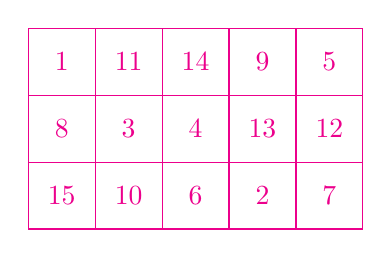
\begin{tikzpicture}[toancuabi,scale=0.85]
			\draw (0,0) grid (5,3);
			\node at (0.5,0.5) {$15$};
			\node at (1.5,0.5) {$10$};
			\node at (2.5,0.5) {$6$};
			\node at (3.5,0.5) {$2$};
			\node at (4.5,0.5) {$7$};
			\node at (0.5,1.5) {$8$};
			\node at (1.5,1.5) {$3$};
			\node at (2.5,1.5) {$4$};
			\node at (3.5,1.5) {$13$};
			\node at (4.5,1.5) {$12$};
			\node at (0.5,2.5) {$1$};
			\node at (1.5,2.5) {$11$};
			\node at (2.5,2.5) {$14$};
			\node at (3.5,2.5) {$9$};
			\node at (4.5,2.5) {$5$};
		\end{tikzpicture}
		\vspace*{-5pt}
	\end{figure}
	Sau đây là một số gợi ý:
	\vskip 0.1cm
	-- Trước tiên ta biết tổng của $15$ số bằng $(15\times16):2=120$. Do đó tổng của mỗi cột (nếu xếp được) là $24$, còn tổng mỗi hàng bằng $40$. Theo suy nghĩ thông thường ta chọn $3$ số cách đều $1$, $8$, $15$ cho cột đầu tiên.
	\vskip 0.1cm
	-- Xem xét $5$ số lớn nhất còn lại ta thấy $10$ và $11$ phải cùng một cột và cùng với số $3$. Ta xếp ba số $3$, $10$, $11$ vào cột hai (tạm thời chưa xếp vào các dòng). 
	\vskip 0.1cm
	-- Tiếp theo, trong các ô ở $3$ cột còn lại (cột thứ $3$ tới cột thứ $5$) ta sẽ xếp số lớn nhất $(14)$ cùng hàng với $1$ và số bé nhất $(2)$ cùng hàng với $15$ (cũng theo nguyên tắc xếp dãn đều). Thấy ngay $14$ và $2$ không thể ở cùng một cột, vì nếu như vậy, ô còn lại phải ghi số $8$ là số ta đã xếp ở cột $1$. Quay lại cột $2$, bằng cách xét từng trường hợp ta chỉ có thể  xếp số $3$ vào ô $G$ (Hình $1$).
	\begin{table}[H]
		\vspace*{-5pt}
		\centering
		\captionsetup{labelformat= empty, justification=centering}
		\renewcommand{\arraystretch}{1.23}
		\begin{tabular}{|c|c|c|c|c|}
			\hline
			$1$ & & $14$& & \\
			$A$&$B$&$C$&$D$& $E$\\
			\hline
			 $8$&$3$&&&\\
			 $F$&$G$&$H$&$I$&$J$\\
			 \hline
			 $15$&&&$2$&\\
			 $K$&$L$&$M$&$N$&$P$\\
			 \hline
		\end{tabular}
		\caption{\small\textit{\color{toancuabi}Hình $1$.}}
		\vspace*{-10pt}
	\end{table}
	-- Tiếp theo do tổng các ô $H$, $I$ và $J$ sẽ bằng $40-(8+3)= 29$ các ô này phải có cả hai số ``lớn" còn lại là $12$ và $13$ và ô còn lại trong $3$ ô này phải là số $4$. Xét $3$ trường hợp cho ô $I$ ta thấy chỉ có thể điền $13$ vào ô $I$.  Khi đó ta điền tiếp được các ô $H$, $J$, $D$, $M$ (Hình $2$)
	\begin{table}[H]
		\vspace*{-5pt}
		\centering
		\captionsetup{labelformat= empty, justification=centering}
		\renewcommand{\arraystretch}{1.23}
		\begin{tabular}{|c|c|c|c|c|}
			\hline
			$1$ & & $14$&$9$ & \\
			$A$&$B$&$C$&$D$& $E$\\
			\hline
			$8$&$3$&$4$&$13$&$12$\\
			$F$&$G$&$H$&$I$&$J$\\
			\hline
			$15$&&$6$&$2$&\\
			$K$&$L$&$M$&$N$&$P$\\
			\hline
		\end{tabular}
		\caption{\small\textit{\color{toancuabi}Hình $2$.}}
		\vspace*{-10pt}
	\end{table}
	-- Chỉ có thể điền $11$ vào ô $B$ và cuối cùng thu được toàn bộ bảng ở Hình $3$.
	\begin{table}[H]
		\vspace*{-5pt}
		\centering
		\captionsetup{labelformat= empty, justification=centering}
		\renewcommand{\arraystretch}{1.23}
		\begin{tabular}{|c|c|c|c|c|}
			\hline
			$1$ &$11$&$14$&$9$&$5$ \\
			$A$&$B$&$C$&$D$& $E$\\
			\hline
			$8$&$3$&$4$&$13$&$12$\\
			$F$&$G$&$H$&$I$&$J$\\
			\hline
			$15$&$10$&$6$&$2$&$7$\\
			$K$&$L$&$M$&$N$&$P$\\
			\hline
		\end{tabular}
		\caption{\small\textit{\color{toancuabi}Hình $3$.}}
		\vspace*{-10pt}
	\end{table}
	Các em cũng có thể đổi chỗ các cột, hoặc các hàng để có một cách điền khác.
	\vskip 0.1cm
	$\pmb{5.}$ Hai bạn cùng chơi một trò tô màu sau đây: các bạn lần lượt tô bằng màu đỏ các ô của một bảng ô vuông ca--rô $4\times 4$. Ở mỗi một bước, các bạn phải tô một ô trắng bằng màu đỏ, sao cho không có hình vuông $2\times 2$ nào bị tô đỏ hết. Bạn nào không đi được bước tiếp theo sẽ bị thua. Hỏi bạn nào sẽ luôn có cách chơi để thắng đối phương: bạn tô đầu tiên hay là người chơi cùng với bạn đó? 
	\begin{figure}[H]
		\vspace*{-5pt}
		\centering
		\captionsetup{labelformat= empty, justification=centering}
		\includegraphics[width= 1\linewidth]{bai5}
		\vspace*{-15pt}
	\end{figure}
	\textit{Lời giải.} Ta đánh số $16$ ô của bàn cờ caro như sau
	\begin{figure}[H]
		\centering
		\vspace*{-5pt}
		\captionsetup{labelformat= empty, justification=centering}
		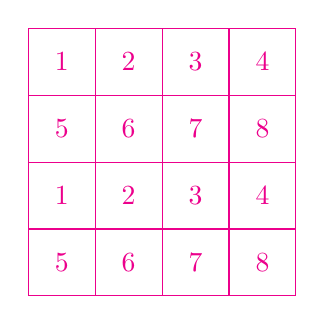
\begin{tikzpicture}[toancuabi,scale=0.85]
			\draw (0,0) grid (4,4);
			\node at (0.5,0.5) {$5$};
			\node at (1.5,0.5) {$6$};
			\node at (2.5,0.5) {$7$};
			\node at (3.5,0.5) {$8$};
			\node at (0.5,1.5) {$1$};
			\node at (1.5,1.5) {$2$};
			\node at (2.5,1.5) {$3$};
			\node at (3.5,1.5) {$4$};
			\node at (0.5,2.5) {$5$};
			\node at (1.5,2.5) {$6$};
			\node at (2.5,2.5) {$7$};
			\node at (3.5,2.5) {$8$};
			\node at (0.5,3.5) {$1$};
			\node at (1.5,3.5) {$2$};
			\node at (2.5,3.5) {$3$};
			\node at (3.5,3.5) {$4$};
		\end{tikzpicture}
		\vspace*{-5pt}
	\end{figure}
	Người chơi thứ hai (đối thủ của người đi trước) sẽ luôn có thể thắng bằng chiến thuật sau đây: hễ người thứ nhất tô màu vào ô nào trong số $16$ ô trong bảng, người chơi thứ hai sẽ tô vào ô có cùng số với ô vừa được người thứ nhất đã tô. Do không có hình vuông $2\times2$ nào trong bàn cờ có $2$ số giống nhau nên người thứ hai không bao giờ bị đẩy vào tình huống thua vì không đi được bước tiếp theo.
	\vskip 0.1cm
	$\pmb{6.}$ Có $31$ người cùng ngồi xung quanh một chiếc bàn tròn. Một số người trong họ là các Hiệp sỹ -- đó là những người luôn nói thật, còn những người còn lại là Lừa dối -- họ luôn nói sai, hơn nữa số người Lừa dối ít nhất là $1$. Người ta hỏi mỗi người trong số họ ``có bao nhiêu người Lừa dối ngồi cạnh anh?" (tức là người ngồi cạnh bên tay trái và bên tay phải). Tất cả mọi người cùng đưa ra câu trả lời như nhau. Hỏi số Hiệp sỹ lớn nhất có thể ngồi xung quanh bàn là bao nhiêu?
	\begin{figure}[H]
		\vspace*{-5pt}
		\centering
		\captionsetup{labelformat= empty, justification=centering}
		\includegraphics[width= 1\linewidth]{bai6}
		\vspace*{-10pt}
	\end{figure}
	\textit{Lời giải.} Giả sử xung quanh bàn có ít nhất $16$ Hiệp sỹ. Khi đó phải có ít  nhất $2$ Hiệp sỹ ngồi cạnh nhau. Hơn nữa vì số người Lừa dối có ít nhất là $1$, nên phải có $2$ Hiệp sỹ ngồi cạnh nhau, và một trong số họ có một người Lừa dối ngồi cạnh. Như vậy, có một Hiệp sỹ đưa ra câu trả lời là ``$1$", và tất cả cũng đã đều trả lời là ``$1$".
	\vskip 0.1cm 
	Vì thế các Hiệp sỹ phải ngồi theo từng cặp, mỗi một cặp Hiệp sỹ được bao quanh bởi các người Lừa dối. Hơn nữa, mỗi một người Lừa dối phải được bao quanh bởi $2$ Hiệp sỹ (vì nếu có một người Lừa dối có $2$ người ngồi cạnh là Hiệp sỹ và Lừa dối khác, thì hóa ra anh ta lại nói thật, điều này là không thể. Do đó chỉ có thể có cách xếp như sau
	\begin{align*}
		\ldots\text{\scriptsize{HHLHHLHHL}}\ldots
	\end{align*}
	(H -- Hiệp sỹ, L -- Lừa dối). Nhưng khi đó thì tổng số người phải là bội số của $3$. Đây là điều mâu thuẫn. Do vậy số Hiệp sỹ không quá $15$.
	\vskip 0.1cm
	Ta sẽ chỉ ra ví dụ khi có đúng $15$ Hiệp sỹ ngồi quanh bàn như sau
	\begin{align*}
		\text{\scriptsize{LHLHLHLHLHLHLHLHLHLHLHLHLHLHLLH}}
	\end{align*}
	(người đầu và người cuối trong dãy trên ngồi cạnh nhau). Khi đó mỗi người ở quanh bàn đều trả lời ``$2$".
\end{multicols}
\newpage
\begingroup
\thispagestyle{toancuabinone}
\blfootnote{$^1$\color{toancuabi}Trường THCS Archimedes, Hà Nội.}
\AddToShipoutPicture*{\put(60,733){\includegraphics[width=17.2cm]{../mathc.pdf}}}
%\AddToShipoutPicture*{\put(-2,733){\includegraphics[width=17.2cm]{../mathl.pdf}}} 
\AddToShipoutPicture*{\put(112,675){\includegraphics[scale=1]{../tieude3.pdf}}} 
\centering
\endgroup
\graphicspath{{../toancuabi/pic/}}
\vspace*{35pt}

\begin{multicols}{2}
	\PIbox{\textbf{\color{toancuabi}Problem} $\pmb{1.}$ How many ways are there to color the regions $A$, $B$, $C$, $D$ in the figure with three different colors, where each region is colored by one color?}	 
	\begin{figure}[H]
		\centering
		\vspace*{-5pt}
		\captionsetup{labelformat= empty, justification=centering}
		\includegraphics[scale=1]{m1}
		\vspace*{-5pt}
	\end{figure}
	\PIbox{\textbf{\color{toancuabi}Rule of Multiplication:} Suppose that we have to do two independent jobs $A$ and $B$, and that there are $m$ ways to do job $A$ and $n$ ways to do job $B$. We cannot do both jobs at the same time, then there are $(m \times n)$ ways to do \textbf{\color{toancuabi}both} jobs.}
	\vskip 0.1cm
	\textit{Solution}: There are $4$ regions to be colored, and there are $3$ ways to color each region. Therefore, the number of colorings is 
	\begin{align*}
		\text{Rule of multiplication: }	3 \times 3\times 3\times 3=81.
	\end{align*}
	\PIbox{\textbf{\color{toancuabi}Problem} $\pmb{2.}$ How many ways are there to color the regions $A$, $B$, $C$, $D$, $E$ in the figure using three different colors such that two adjacent regions have different colors?	} 
	\begin{figure}[H]
		\centering
		\vspace*{-5pt}
		\captionsetup{labelformat= empty, justification=centering}
		\includegraphics[scale=1]{m2}
		\vspace*{-10pt}
	\end{figure}
	\textit{Solution}: We color in the order $A \to B \to C \to D \to E$. There are $3$ ways to color region $A$. After that, there are $2$ ways to color $B$ with a different color. Then there are $2$ ways to color $C$ with a color different from $B$, and so on ...
	\vskip 0.1cm   
	According to the rule of multiplication, the number of colorings is given by
	\begin{align*}
		\text{Rule of multiplication: } 3 \times 2^4= 48.
	\end{align*}
	\PIbox{\textbf{\color{toancuabi}Problem} $\pmb{3.}$ How many ways are there to put $8$ rooks on a chessboard so that they do not attack each other? 
	\vskip 0.1cm
	(\textit{Note that two rooks on the same row or column attack each other.})}
	\begin{figure}[H]
		\centering
%		\vspace*{-5pt}
		\captionsetup{labelformat= empty, justification=centering}
		\includegraphics[width=1\linewidth]{co}
		\vspace*{-10pt}
	\end{figure}
	\textit{Solution}:
	\vskip 0.1cm 
	$\circ$ Step $1$: Put the $1^{\text{st}}$ rook on the $1^{\text{st}}$ row: $8$ ways
	\vskip 0.1cm
	$\circ$ Step $2$: Put the $2^{\text{nd}}$ rook on the $2^{\text{nd}}$ row: $7$ ways
	\vskip 0.1cm
	$\circ$ $\ldots$
	\vskip 0.1cm
	$\circ$ Step $8$: Put the $8^{\text{th}}$ rook on the $8^{\text{th}}$ row: $1$ way
	\vskip 0.1cm
	By the rule of multiplication, there are 
	\begin{align*}
		8\times7\times6\times\ldots\times1=40320
	\end{align*}
	ways to put $8$ rooks on a chessboard such that they do not attack each other.
	\vskip 0.1cm
	\PIbox{\textbf{\color{toancuabi}Problem} $\pmb{4.}$ There are $5$ {\color{green}green balls} numbered from $1$ to $5$, $6$ {\color{red}red balls} numbered from $1$ to $6$, and $7$ {\color{yellow}yellow balls} numbered from $1$ to $7$. How many ways are there to choose $3$ balls such that they have different colors and numbers?}
	\begin{figure}[H]
		\centering
		\vspace*{-5pt}
		\captionsetup{labelformat= empty, justification=centering}
		\includegraphics[width=1\linewidth]{bong}
		\vspace*{-10pt}
	\end{figure}
	\textit{Solution:}
	\vskip 0.1cm 
	$\circ$ First, we choose a {\color{green}green ball}. There are $5$ available choices. 
	\vskip 0.1cm
	$\circ$ Next, we choose a {\color{red}red ball}. The number on this {\color{red}red ball} is different from that of the {\color{green}green ball}, so there are $6-1=5$ available choices. 
	\vskip 0.1cm
	$\circ$ Finally, we choose a {\color{yellow}yellow ball}, and there are $7-2=5$ available choices. 
	\vskip 0.1cm
	According to the rule of multiplication, the number of ways to choose $3$ balls of different colors and different numbers is: 
	\begin{align*}
		5\times5\times5=125.
	\end{align*}
	\PIbox{\textbf{\color{toancuabi}Problem} $\pmb{5.}$ How many even $4$--digit numbers with distinct digits are there?}
	\vskip 0.1cm
	\textit{Solution}:  Let’s write an even $4$--digit number as $\overline{abcd}$ where $a\ne 0$, the $4$ digits $a$, $b$, $c$, $d$ are pairwise distinct, and $d$ is in the set $\{0,2,4,6,8\}$.
	\vskip 0.1cm
	We consider two cases:
	\vskip 0.1cm
	\textit{Case} $1$: $d=0$. There are $9$ ways to choose $a$, then $8$ ways to choose $b$ and then $7$ ways to choose $c$. Therefore, there are $1\times 9\times8\times7$ choices of the number $\overline{abcd}$.
	\vskip 0.1cm
	\textit{Case} $2$: $d\ne0$. There are $4$ ways to choose $d$. For each choice of $d$, there are $8$ ways to choose $a$ ($a\ne0$ and $a\ne d$), then $8$ ways to choose $b$ and then $7$ ways to choose $c$. Therefore, there are $4
	\times8\times8\times7$ choices of the number $\overline{abcd}$.
	\vskip 0.1cm
	Thus, there are 
	\begin{align*}
		1\times9\times8\times7+4\times8\times8\times7 = 2296
	\end{align*}
	numbers that satisfy the requirement of the problem.
	\vskip 0.1cm
	\PIbox{\textbf{\color{toancuabi}Exercise} $\pmb{1.}$ How many ways are there to color the regions $A$, $B$, $C$, $D$ in the figure with one color for each region, given that there are three different colors and no two adjacent regions have the same color?}
	\begin{figure}[H]
		\centering
		\vspace*{-5pt}
		\captionsetup{labelformat= empty, justification=centering}
		\includegraphics[scale=1]{m3}
		\vspace*{-5pt}
	\end{figure}
	\vskip 0.1cm
	\PIbox{\textbf{\color{toancuabi}Exercise} $\pmb{2.}$ How many ways are there to color the sides of a pentagon with three different colors such that no two adjacent sides have the same color?}
	\vskip 0.2cm
	\PIbox{{\centerline{\textbf{\color{toancuabi}New words}}}
		\vskip 0.2cm
		{\color{toancuabi}Adjacent(adj):} bên cạnh, cạnh nhau
		\vskip 0.1cm
		{\color{toancuabi}Case:} trường hợp 
		\vskip 0.1cm
		{\color{toancuabi}Color (v):} tô màu 
		\vskip 0.1cm
		{\color{toancuabi}Different:} khác 
		\vskip 0.1cm
		{\color{toancuabi}Region:} vùng, miền
		\vskip 0.1cm
		{\color{toancuabi}Rook (Chess):} quân Xe trên bàn cờ Vua  
		\vskip 0.1cm
		{\color{toancuabi}Rule of Multiplication:} Quy tắc Nhân
		\vskip 0.1cm
		{\color{toancuabi}Way:} con đường, cách (thực hiện) }
\end{multicols}
%	 \newpage
%
%	 \setcounter{figure}{0}
%	 \thispagestyle{thachthuctoanhocnone}
\pagestyle{thachthuctoanhoc}
\everymath{\color{thachthuctoanhoc}}
\graphicspath{{../thachthuctoanhoc/pic/}}
\begingroup
\AddToShipoutPicture*{\put(0,616){\includegraphics[width=19.3cm]{../thachthuctoanhoc/bannerthachthuc}}}
\centering
\vspace*{4cm}
\endgroup
\vspace*{-8pt}
\begin{tBox}
	\begin{itemize}[leftmargin = 13pt, itemsep = 1.0pt] 
				\item Mỗi bài toán đề xuất (kèm theo lời giải) cần được nêu rõ là bài sáng tác hay bài sưu tầm.
%		\item Mỗi bài toán đề xuất (kèm theo lời giải) cần được nêu rõ là bài sáng tác hay bài sưu tầm (nếu là bài sưu tầm, cần ghi rõ nguồn).
		\item Bài giải cho mỗi bài toán cần được trình bày trong một file riêng hoặc
		một tờ giấy riêng.
		\item  Người đề xuất bài toán hoặc gửi bài giải cho các bài toán trong mục ``Thách thức kỳ này" cần ghi rõ họ, đệm, tên và nơi làm việc/học tập, số điện thoại liên hệ. Nếu là học sinh (hoặc sinh viên) cần ghi rõ là học sinh lớp mấy (hoặc sinh viên năm thứ mấy).
		\item Các bài toán trong mục Thách thức kỳ này hướng tới các độc giả là học sinh phổ thông; được phân chia thành các mức độ $B$, $A$, và được sắp xếp theo độ khó tăng dần, theo đánh giá chủ quan của Ban biên tập. Các bài toán mức độ $B$ không đòi hỏi các kiến thức vượt quá chương trình môn Toán cấp THCS; các bài toán mức độ $A$ không đòi hỏi các kiến thức vượt quá chương trình môn Toán cấp THPT.
		\item Cách thức gửi bài toán đề xuất hoặc lời giải: gửi file thu được bằng cách scan, ảnh chụp (rõ nét) của bản viết tay, hoặc được soạn thảo bằng các phần mềm Latex, Word tới \url{bbt@pi.edu.vn} hoặc gửi qua đường bưu điện tới Tòa soạn (xem địa chỉ tại bìa $2$).
		\item Hạn gửi lời giải cho các bài toán P$641$--P$650$: trước ngày $15/11/2022$.
	\end{itemize}
\end{tBox}
\begin{center}
	\vspace*{-5pt}
	\textbf{\color{thachthuctoanhoc}\color{thachthuctoanhoc}THÁCH THỨC KỲ NÀY}
	\vspace*{-5pt}
\end{center}
\begin{multicols}{2}
	\setlength{\abovedisplayskip}{4pt}
	\setlength{\belowdisplayskip}{4pt}
	{\color{thachthuctoanhoc}{\usefont{T5}{qag}{b}{n} P641.}}
	(Mức $B$) Tại mỗi đỉnh của một đa giác lồi $18$ cạnh ở Hình dưới đây, người ta ghi một số, sao cho số được ghi ở mỗi đỉnh bằng tổng hai số được ghi ở hai đỉnh kề với nó.
	\begin{figure}[H]
		\vspace*{-5pt}
		\centering
		\captionsetup{labelformat= empty, justification=centering}
		\definecolor{ffvvqq}{rgb}{1,0.3333333333333333,0}
		\definecolor{qqqqffa}{rgb}{0,0,1}
		\definecolor{qqzzff}{rgb}{0,0.6,1}
		\begin{tikzpicture}[line cap=round,line join=round,>=triangle 45,x=1cm,y=1cm,scale=0.42]
			\draw (1.401115339869085,5.50644760016908136) node[anchor=north west] {$X$};
			\draw (1.4408759814898973,-0.7306378725360659) node[anchor=north west] {$Y$};
			\draw (-7.8444170535279,2.5008856260029945) node[anchor=north west] {$S$};
			\draw [color=qqzzff] (0.0915547437082469,-1.9784020259611625)--(1.3147607160299626,-0.9781184915188108);
			\draw [color=qqzzff] (1.3147607160299626,-0.9781184915188108)--(2.122081224105652,0.3802016464606015); 
			\draw [color=qqzzff] (2.122081224105652,0.3802016464606015)--(2.4161414998796458,1.932724932666551); 
			\draw [color=qqzzff] (2.4161414998796458,1.932724932666551)--(2.1614735342261406,3.4921941459791768);
			\draw [color=qqzzff] (2.1614735342261406,3.4921941459791768)--(1.38879404230183,4.87051428395859);
			\draw [color=qqzzff] (1.38879404230183,4.87051428395859)--(0.19129957436757605,5.901439596125702);
			\draw [color=qqzzff] (0.19129957436757605,5.901439596125702)--(-1.2865743636076452,6.4606252749959765);
			\draw [color=qqzzff] (-1.2865743636076452,6.4606252749959765)--(-2.866574363607645,6.480625274995977);
			\draw [color=qqzzff] (-2.866574363607645,6.480625274995977)--(-4.358129107315893,5.959027300957139);
			\draw [color=qqzzff] (-4.358129107315893,5.959027300957139)--(-5.581335079637608,4.958743766514788);
			\draw [color=qqzzff] (-5.581335079637608,4.958743766514788)--(-6.388655587713298,3.600423628535374);
			\draw [color=qqzzff] (-6.388655587713298,3.600423628535374)--(-6.682715863487291,2.0479003423294264);
			\draw [color=qqzzff] (-6.682715863487291,2.0479003423294264)--(-6.428047897833785,0.4884311290167975);
			\draw [color=qqzzff] (-6.428047897833785,0.4884311290167975)--(-5.655368405909476,-0.889889008962613);
			\draw [color=qqzzff] (-5.655368405909476,-0.889889008962613)--(-4.457873937975224,-1.9208143211297237);
			\draw [color=qqzzff] (-4.457873937975224,-1.9208143211297237)--(-2.98,-2.48);
			\draw [color=qqzzff] (-2.98,-2.48)--(-1.4,-2.5);
			\draw [color=qqzzff] (-1.4,-2.5)--(0.0915547437082469,-1.9784020259611625);
			\draw [fill=qqqqffa] (-2.98,-2.48) circle (1.6pt);
			\draw [fill=qqqqffa] (-1.4,-2.5) circle (1.6pt);
			\draw [fill=qqqqffa] (0.0915547437082469,-1.9784020259611625) circle (1.6pt);
			\draw [fill=qqqqffa] (1.3147607160299626,-0.9781184915188108) circle (1.6pt);
			\draw [fill=qqqqffa] (2.122081224105652,0.3802016464606015) circle (1.6pt);
			\draw [fill=qqqqffa] (2.4161414998796458,1.932724932666551) circle (1.6pt);
			\draw [fill=qqqqffa] (2.1614735342261406,3.4921941459791768) circle (1.6pt);
			\draw [fill=qqqqffa] (1.38879404230183,4.87051428395859) circle (1.6pt);
			\draw [fill=qqqqffa] (0.19129957436757605,5.901439596125702) circle (1.6pt);
			\draw [fill=qqqqffa] (-1.2865743636076452,6.4606252749959765) circle (1.6pt);
			\draw [fill=qqqqffa] (-2.866574363607645,6.480625274995977) circle (1.6pt);
			\draw [fill=qqqqffa] (-4.358129107315893,5.959027300957139) circle (1.6pt);
			\draw [fill=qqqqffa] (-5.581335079637608,4.958743766514788) circle (1.6pt);
			\draw [fill=qqqqffa] (-6.388655587713298,3.600423628535374) circle (1.6pt);
			\draw [fill=qqqqffa] (-6.682715863487291,2.0479003423294264) circle (1.6pt);
			\draw [fill=qqqqffa] (-6.428047897833785,0.4884311290167975) circle (1.6pt);
			\draw [fill=qqqqffa] (-5.655368405909476,-0.889889008962613) circle (1.6pt);
			\draw [fill=qqqqffa] (-4.457873937975224,-1.9208143211297237) circle (1.6pt);
		\end{tikzpicture}
		\vspace*{-5pt}
	\end{figure}
	Biết rằng, số được ghi ở đỉnh $X$ là $20$, và số được ghi ở đỉnh $Y$ là $22$. Hãy tìm số được ghi ở đỉnh $S$. 
	\vskip 0.05cm
	\hfill	\textit{Bùi Văn Biên, France (st)}
	\vskip 0.05cm
	{\color{thachthuctoanhoc}{\usefont{T5}{qag}{b}{n} P642.}}
	(Mức $B$) Cho $x,y$ là các số nguyên dương thoả mãn $y^2+x-1$ chia hết cho \linebreak $xy+1$. Chứng minh rằng, tồn tại số tự nhiên $z$ sao cho $x+y+z+xyz$ là số chính phương.
	\begin{flushright}
		\textit{Nguyễn Đức Tấn, Tp. Hồ Chí Minh}
	\end{flushright}
	{\color{thachthuctoanhoc}{\usefont{T5}{qag}{b}{n} P643.}}
	(Mức $B$) Người ta lần lượt ghi các số lên bảng, theo quy tắc: Ở mỗi lần ghi, chỉ ghi một số, và nếu số được ghi ở lần thứ $k$ ($k\in\mathbb N^*$) là $x\neq-1$, thì ở lần thứ $k+1$ ghi số $\dfrac{x-1}{x+1}$. Hãy tìm số nhỏ nhất cần ghi ở lần thứ nhất, sao cho trong quá trình ghi số lên bảng theo quy tắc trên, ta ghi được số $-\dfrac1{2023}$. 
	\begin{flushright}
		\textit{Phùng Chí Tự, Hà Nội}
	\end{flushright}
	{\color{thachthuctoanhoc}{\usefont{T5}{qag}{b}{n} P644.}}
	(Mức $B$) Xét tam giác $ABC$ có các góc $B,C$ nhọn. Gọi $H$ là chân đường cao kẻ từ $A$ của tam giác đó.  Chứng minh rằng, $ABC$ là tam giác vuông tại $A$ khi và chỉ khi 
	\begin{align*}
		\dfrac{HB^3}{AB^4}+\dfrac{HC^3}{AC^4}=\dfrac1{BC}\cdot
	\end{align*} 
	\begin{center} 
		\definecolor{ffqqqq}{rgb}{1,0,0}
		\definecolor{qqzzff}{rgb}{0,0.6,1}
		\definecolor{qqqqff}{rgb}{0,0,1}
		\definecolor{qqqqffa}{rgb}{1,1,1}
		\definecolor{cqcqcq}{rgb}{0.7529411764705882,0.7529411764705882,0.7529411764705882}
		\begin{tikzpicture}[line cap=round,line join=round,>=triangle 45,x=1cm,y=1cm, scale=0.6]
			\draw (-2.8771572875253812,-2) -- (-2.8771572875253812,-1.7171572875253809) -- (-3.16,-1.7171572875253809) -- (-3.16,-2) -- cycle; 
			\draw [color=qqzzff] (-3.16,4.66)-- (-5.54,-2);
			\draw [color=qqzzff] (-5.54,-2)-- (2,-2);
			\draw [color=qqzzff] (2,-2)-- (-3.16,4.66);
			\draw [,color=ffqqqq] (-3.16,4.66)-- (-3.16,-2);
			\draw [fill=qqqqffa] (-3.16,4.66) circle (1.6pt);
			\draw[color=qqqqff] (-3.18,5.11) node {$A$};
			\draw [fill=qqqqffa] (-5.54,-2) circle (1.6pt);
			\draw[color=qqqqff] (-5.7,-2.5) node {$B$};
			\draw [fill=qqqqffa] (2,-2) circle (1.6pt);
			\draw[color=qqqqff] (2,-2.5) node {$C$};
			\draw [fill=qqqqffa] (-3.16,-2) circle (1.6pt);
			\draw[color=qqqqff] (-3.18,-2.5) node {$H$};
		\end{tikzpicture}
	\end{center}
	\begin{flushright}
		\textit{Trần Quang Hùng, Hà Nội}
	\end{flushright}
	{\color{thachthuctoanhoc}{\usefont{T5}{qag}{b}{n} P645.}}
	(Mức $B$) Cho $a,b,c$ là các số thực dương thoả mãn $abc=1$. Chứng minh rằng 
	\begin{align*}
		\dfrac{a}{a\!+\!b^{3} c\!+\!b}+\dfrac{b}{b\!+\!c^{3} a\!+\!c}+\dfrac{c}{c\!+\!a^{3} b\!+a} \ge 1.
	\end{align*}
	\begin{flushright}
		\textit{Đào Văn Nam, Hà Nội}
	\end{flushright}
	{\color{thachthuctoanhoc}{\usefont{T5}{qag}{b}{n} P646.}}
	(Mức $B$) Chứng minh rằng, trong mỗi bát giác lồi, luôn có ít nhất ba đường chéo, mà độ dài của chúng đôi một khác nhau. 
	\vskip 0.05cm
	(Bát giác là một đa giác có $8$ cạnh.)
	\begin{flushright}
		\textit{Phạm Nhật Nguyệt, Hải Phòng}
	\end{flushright}
	{\color{thachthuctoanhoc}{\usefont{T5}{qag}{b}{n} P647.}}
	(Mức $A$) Cho số nguyên $n\ge2$, và cho $n$ điểm phân biệt $A_1,\ldots,A_n$ cùng nằm trên một đường tròn, theo chiều kim đồng hồ. Một dãy điểm  $A_{k_1},\ldots,A_{k_t}$, gồm ít nhất hai điểm  (trong $n$ điểm đó), không có hai điểm nào trùng nhau, được gọi là một {\it đường đi}, nếu đường gấp khúc $A_{k_1}\ldots A_{k_t}$ (gồm $t-1$ đoạn thẳng) không tự cắt.  Hỏi, có tất cả bao nhiêu đường đi?
	\begin{flushright}
		\textit{Nguyễn Tường Thanh, Nghệ An (st)}
	\end{flushright}
	{\color{thachthuctoanhoc}{\usefont{T5}{qag}{b}{n} P648.}}
	(Mức $A$) Xét số thực $a$ và xét tất cả các hàm số $f: \mathbb R \rightarrow \mathbb R,$ thỏa mãn
	\begin{align*}
		f(a x+y+f(x+y))+f(x y)=y f(x)
	\end{align*}
	với mọi $x,y\in\mathbb R$. 
	\vskip 0.05cm
	$a)$ Tìm tất cả các số thực $a$, sao cho trong các hàm số $f$, tồn tại một hàm là đơn ánh từ $\mathbb R$ đến $\mathbb R$. 
	\vskip 0.05cm
	$b)$ Khi $a=2$, tìm tất cả các hàm số $f$ có $f(0)=0$. 
	\begin{flushright}
		\textit{Lê Phúc Lữ, Tp. Hồ Chí Minh}
	\end{flushright}
	{\color{thachthuctoanhoc}{\usefont{T5}{qag}{b}{n} P649.}}
	(Mức $A$) Cho tam giác $A B C$ và điểm $D$ cố định nằm trên $B C$ ($D$ khác $B,C$). Một đường tròn $(O)$ thay đổi,  đi qua $B, C$ và cắt các cạnh $A B, A C$ tương ứng tại $E, F$. Gọi $G$ là giao điểm của $B F$ và $A D$. Chứng minh rằng, đường thẳng $G E$ luôn đi qua một điểm cố định.
	\begin{center}
		\definecolor{ffqqqq}{rgb}{1,0,0}
		\definecolor{qqzzff}{rgb}{0,0.6,1}
		\definecolor{qqqqff}{rgb}{0,0,1}
		\definecolor{qqqqffa}{rgb}{1,1,1}
		\begin{tikzpicture}[line cap=round,line join=round,>=triangle 45,x=1cm,y=1cm,scale=0.6]
			\draw [color=qqzzff] (-4.81309,-1)-- (-2.9915435035522586,4.9363824736365585);
			\draw [color=qqzzff] (-2.9915435035522586,4.9363824736365585)-- (2.16949,-1);
			\draw [color=qqzzff] (2.16949,-1)-- (-4.81309,-1);
			\draw [thachthuctoanhoc] (-1.3218,-0.16393583791880353) circle (3.590001273985364cm);
			\draw [] (-4.81309,-1)-- (-1.6642556805547637,3.409694424723417);
			\draw [] (-2.9915435035522586,4.9363824736365585)-- (-0.3604269142578283,-1);
			\draw [,color=ffqqqq] (-6.227177601372653,1.9518434021508382)-- (2.997592242483252,3.9372366050655776);
			\draw [fill=qqqqffa] (-2.9915435035522586,4.9363824736365585) circle (1.6pt);
			\draw[color=qqqqff] (-3.0725009370690106,5.432246753926664) node {$A$};
			\draw [fill=qqqqffa] (-4.81309,-1) circle (1.6pt);
			\draw[color=qqqqff] (-5.177394208504555,-1.1455447193094175) node {$B$};
			\draw [fill=qqqqffa] (2.16949,-1) circle (1.6pt);
			\draw[color=qqqqff] (2.531407750174166,-1.2062627944469815) node {$C$};
			\draw [fill=qqqqffa] (-1.3218,-0.16393583791880353) circle (1.6pt);
			\draw[color=qqqqff] (-1.721554748380367,-0.3966884592794637) node {$O$};
			\draw [fill=qqqqffa] (-3.7432966215398427,2.4864345624380344) circle (1.6pt);
			\draw[color=qqqqff] (-4.064229497649219,2.801130164632231) node {$E$};
			\draw [fill=qqqqffa] (-1.6642556805547637,3.409694424723417) circle (1.6pt);
			\draw[color=qqqqff] (-1.5545490586299158,3.873816158729192) node {$F$};
			\draw [fill=qqqqffa] (-0.3604269142578283,-1) circle (1.6pt);
			\draw[color=qqqqff] (-0.36042691425782825,-1.507459586342921) node {$D$};
			\draw [fill=qqqqffa] (-2.0657079453674543,2.847492151010585) circle (1.6pt);
			\draw[color=qqqqff] (-2.161729810005554,2.11658235542766) node {$G$};
		\end{tikzpicture}
	\end{center}
	\begin{flushright}
		\textit{Phạm Vĩnh Minh, Đồng Tháp}
	\end{flushright}
	{\color{thachthuctoanhoc}{\usefont{T5}{qag}{b}{n} P650.}}
	(Mức $A$) Cho $p$ là một số nguyên tố có dạng $4k+3$, $k\in\mathbb N$.  Xét dãy số Fibonacci $(F_n)$, xác định bởi: $F_0=0$, $F_1=1$, và 
	\begin{align*}
		F_{n+2}=F_{n+1}+F_n\quad\text{\color{black}với mọi } n\ge0.
	\end{align*}
	Chứng minh rằng, không tồn tại các số nguyên dương $m,\,n$, với $n\ge 5$, sao cho \linebreak$F_n=p^m$.
	\begin{flushright}
		\textit{Nguyễn Song Minh, Hà Nội (st)}
	\end{flushright}
\end{multicols}
%\begin{center}
%	{\large{\textbf{\color{thachthuctoanhoc}GIẢI BÀI KỲ TRƯỚC}}}
%\end{center}
%\begin{multicols}{2}
%	\setlength{\abovedisplayskip}{4pt}
%	\setlength{\belowdisplayskip}{4pt}
%	{\color{thachthuctoanhoc}{\usefont{T5}{qag}{b}{n} P611.}}
%	(Mức $B$) Cho $A,B,C$ là các chữ số khác $0$ sao cho $\overline{CCA}+\overline{B2B}=\overline{A88}$. Hãy tìm số $\overline{ABC}$.
%	\vskip 0.05cm
%	\textbf{Lời giải} (\textit{dựa theo lời giải của bạn Phùng Việt Cường, lớp $10$T$2$, trường THPT chuyên Lê Hồng Phong, tỉnh Nam Định})\textbf{.}
%	\vskip 0.05cm
%	Viết lại giả thiết của bài ra dưới dạng:
%	\begin{align*}
%		\begin{array}{l}
%			\underline \begin{array}{l}
%				\overline {CCA} \\
%				\overline {B2B} 
%			\end{array} \\
%			\overline {A88} 
%		\end{array}
%	\end{align*}
%	Theo quy tắc ``cộng dọc", từ phép cộng ở hàng trăm, suy ra
%	\begin{align*}
%		C + B \le A \le 9.
%	\end{align*}
%	Do đó, $B < 9$ (vì $C > 0$); suy ra, $A + B < 18$. Vì thế, từ phép cộng ở hàng đơn vị, ta được
%	\begin{align*}
%		A + B = 8. \tag{$1$}
%	\end{align*}                                                                  
%	Do đó, từ phép cộng ở hàng chục, với lưu ý $C + 2 \le 11$, ta có $C + 2 = 8$. Vì thế, $C = 6$. Do đó, từ phép cộng ở hàng trăm, ta có
%	\begin{align*}
%		6 + B = A, \text{\color{black} hay }A - B = 6. \tag{$2$}
%	\end{align*}
%	Từ ($1$) và ($2$), ta được $A = 7$ và $B = 1$.
%	\vskip 0.05cm
%	Vậy, $\overline {ABC} \,\, = \,\,716$.
%	\vskip 0.05cm
%	\textbf{Bình luận và Nhận xét}
%	\vskip 0.05cm
%	Rất tiếc, trong số các lời giải Tạp chí đã nhận được từ bạn đọc, có ba lời giải không đúng, do người giải bài đã mắc một trong các lỗi sau:
%	\vskip 0.05cm
%	$\bullet$  Với $a$, $b$, $c$, $x$, $y$, $z$, $u$, $v$, $t$ là các số nguyên, từ
%	\begin{align*}
%		ax + by + cz = au + bv + ct,
%	\end{align*}
%	suy ra, $x = u$, $y = v$ và $z = t$.
%	\vskip 0.05cm
%	$\bullet$  Khi xét phép cộng ở hàng chục của phép ``cộng dọc", quên trường hợp ``có nhớ từ phép cộng ở hàng đơn vị".
%	\begin{flushright}
%		\textbf{Lê Huy}
%	\end{flushright}
%	{\color{thachthuctoanhoc}{\usefont{T5}{qag}{b}{n} P612.}}
%	(Mức $B$) Chứng minh biểu thức sau nhận giá trị nguyên, với mọi giá trị nguyên dương của $n$:
%	\begin{align*}
%		A\!=\!\dfrac{\left(2^4\!+\!\dfrac14\right)\!\left(4^4\!+\!\dfrac14\right)\!\cdots\! \left((2n)^4\!+\!\dfrac14\right)}{\left(1^4\!+\!\dfrac14\right)\left(3^4\!+\!\dfrac14\right)\!\cdots\! \left((2n\!-\!1)^4\!+\!\dfrac14\right)}.
%	\end{align*}
%	\textbf{Lời giải} (\textit{dựa theo tuyệt đại đa số lời giải Tạp chí đã nhận được từ bạn đọc})\textbf{.}
%	\vskip 0.05cm
%	Với mọi số nguyên dương $m$, ta có:
%	\begin{align*}
%		{m^4}\, + \,\,\frac{1}{4}\,\, = \,\,{m^4}\, + \,\,2 \cdot {m^2} \cdot \frac{1}{2}\,\, + \,\,\frac{1}{4}\,\, - \,\,{m^2}\, = \,\,{\left( {{m^2}\, + \,\,\frac{1}{2}} \right)^2}\, - \,\,{m^2}\\
%		\,\,\,\,\,\,\,\,\,\,\,\,\,\,\,\, = \,\,\left( {{m^2}\, - \,\,m\,\, + \,\,\frac{1}{2}} \right)\left( {{m^2}\, + \,\,m\,\, + \,\,\frac{1}{2}} \right).
%	\end{align*}
%	Do đó, với mọi số nguyên dương $k$, ta có:
%	\begin{align*}
%		{\left( {2k} \right)^4}\, + \,\,\frac{1}{4}\,\, = \,\,\left( {{{\left( {2k} \right)}^2}\, - \,\,2k\,\, + \,\,\frac{1}{2}} \right)\left( {{{\left( {2k} \right)}^2}\, + \,\,2k\,\, + \,\,\frac{1}{2}} \right);
%	\end{align*}
%	\begin{align*}
%			{\left( {2k\,\, - \,\,1} \right)^4}\, + \,\,\frac{1}{4}\,\, = \,\,\left( {{{\left( {2k\,\, - \,\,1} \right)}^2}\, - \,\,\left( {2k\,\, - \,\,1} \right)\,\, + \,\,\frac{1}{2}} \right)\left( {{{\left( {2k\,\, - \,\,1} \right)}^2}\, + \,\,\left( {2k\,\, - \,\,1} \right)\,\, + \,\,\frac{1}{2}} \right)\\
%			\,\,\,\,\,\,\,\,\,\,\,\,\,\,\,\,\,\,\,\,\,\,\,\,\,\,\,\,\,\, = \,\,\left( {{{\left( {2\left( {k\,\, - \,\,1} \right)} \right)}^2}\, + \,\,2\left( {k\,\, - \,\,1} \right)\,\, + \,\,\frac{1}{2}} \right)\left( {{{\left( {2k} \right)}^2}\, - \,\,2k\,\, + \,\,\frac{1}{2}} \right).
%	\end{align*}
%	Suy ra
%	\begin{align*}
%		\frac{{{{\left( {2k} \right)}^4}\, + \,\,\frac{1}{4}}}{{{{\left( {2k\,\, - \,\,1} \right)}^4}\, + \,\,\frac{1}{4}}}\,\, = \,\,\frac{{{{\left( {2k} \right)}^2}\, + \,\,2k\,\, + \,\,\frac{1}{2}}}{{{{\left( {2\left( {k\,\, - \,\,1} \right)} \right)}^2}\, + \,\,2\left( {k\,\, - \,\,1} \right)\,\, + \,\,\frac{1}{2}}}
%	\end{align*}
%	với mọi số nguyên dương $k$.
%	\vskip 0.05cm
%	Do đó
%	
%	Vì vậy, biểu thức A nhận giá trị nguyên tại mọi giá trị nguyên dương của n.
%	Bình luận và Nhận xét
%	Tất cả các lời giải Tạp chí nhận được từ bạn đọc đều là lời giải đúng.
%	Hà Thanh
%	P613. (Mức B) Cho n là một số nguyên dương. Chứng minh rằng, trong ba số n,   và  , có ít nhất hai số không phải là số chính phương.
%	Lời giải (phỏng theo cách giải của bạn Trần Việt Anh, lớp 8C1, trường TH, THCS&THPT Archimedes, Đông Anh, Tp. Hà Nội).
%	Trước hết, dễ dàng chứng minh được Nhận xét sau:
%	Nhận xét 1: Với mọi số nguyên dương a, số dư trong phép chia   cho 5 chỉ có thể là 0, 1, hoặc 4.
%	Từ đó, ta có:
%	Nhận xét 2:   là số không chính phương.
%	Chứng minh. Giả sử ngược lại,   là số chính phương.
%	Khi đó, tồn tại số nguyên dương m, sao cho
%	hay                                                  (1)
%	Từ Nhận xét 1 suy ra, số dư trong phép chia   cho 5 sẽ là 4, 1, hoặc 2. Điều này mâu thuẫn với (1), do 15n chia hết cho 5. Mâu thuẫn nhận được cho thấy giả sử ở trên là sai; vì thế, Nhận xét 2 được chứng minh.
%	Tiếp theo, giả sử n và   cùng là số chính phương. Khi đó, tồn tại các số nguyên dương x, y, sao cho   và   hay   Từ đây, ta có:
%	;                                                                 (2)
%	suy ra,                                                                                                                         (3)
%	Theo Nhận xét 1,   và  
%	Vì thế, từ (3) suy ra
%	
%	Do đó,   suy ra,   (do 5 là số nguyên tố). Vì thế
%	
%	do đó, từ (2) suy ra,   là điều vô lí. Điều vô lí này cho thấy, trong hai số n và   chỉ có tối đa một số là số chính phương. Từ đây và Nhận xét 2, hiển nhiên ta có điều phải chứng minh theo yêu cầu đề bài.
%	Bình luận và Nhận xét
%	Rất tiếc, trong số các lời giải Tạp chí đã nhận được từ bạn đọc, có một lời giải sai, do người giải bài đã ngộ nhận rằng, ``cả ba số đồng thời là số chính phương" là khẳng định ngược lại với khẳng định cần chứng minh theo yêu cầu đề bài.
%	Lưu Thị Thanh Hà
%	P614. (Mức B) Cho a, b là các số nguyên dương, thỏa mãn
%	
%	Chứng minh rằng, 4b + 1 là một số chính phương.
%	(Với x là một số thực, {x} = x - [x], trong đó, [x] là số nguyên lớn nhất không vượt quá x. {x} được gọi là phần lẻ của số thực x.)
%	Lời giải (dựa theo cách giải của bạn Nguyễn Đức Khải, lớp 10T2, trường THPT chuyên Lê Hồng Phong, tỉnh Nam Định).
%	Viết lại hệ thức của đề bài dưới dạng:
%	
%	Từ đó, suy ra
%	
%	Vì thế, đặt   ta có   và
%	;
%	suy ra
%	(1)
%	Do đó
%	
%	Vì thế, đặt   ta có   và
%	
%	Do đó
%	(2)
%	Suy ra,   (do  ).                                                                                                   (3)
%	Vì   nên hoặc   hoặc   là số vô tỉ.
%	Nếu   thì từ (1) suy ra,   (do  ) và   là số chính phương, là điều vô lí, do
%	
%	Vì vậy,   là số vô tỉ. Kết hợp với (3) suy ra, x = 0 hoặc y = 0.
%	Nếu y = 0 thì   (suy ra từ định nghĩa của y) và đồng thời,   (theo (2)). Do đó
%	;
%	suy ra
%	
%	là điều vô lí, do  
%	Do đó, x = 0. Vì thế, từ định nghĩa của y và (2), suy ra
%	
%	Do đó
%	
%	là một số chính phương.
%	Ta có điều phải chứng minh theo yêu cầu đề bài.
%	Bình luận và Nhận xét
%	
%	Lưu Thị Thanh Hà
%	P615. (Mức B) Cho tam giác ABC vuông tại A. Một điểm D di chuyển trên tia CA. Gọi E là hình chiếu vuông góc của C trên đường thẳng BD; F là giao điểm của AE và BC. Chứng minh rằng, đường thẳng DF luôn đi qua một điểm cố định.
%	Lời giải ().
%	
%	Bình luận và Nhận xét
%	
%	Hạ Vũ Anh
%	P616. (Mức B) Xét các số dương a, b, c thỏa mãn a + b + c = 4. Tìm giá trị nhỏ nhất của biểu thức
%	
%	Lời giải (dựa theo lời giải của bạn Trần Việt Anh, lớp 8C1, trường TH, THCS&THPT Archimedes, Đông Anh, Tp. Hà Nội).
%	Do a, b, c có vai trò như nhau trong biểu thức P nên không mất tính tổng quát, có thể giả sử a = max{a, b, c}.
%	Xét hai trường hợp sau:
%	• Trường hợp 1: a > 2.
%	Khi đó,   suy ra
%	
%	Do đó
%	
%	Vì thế
%	
%	• Trường hợp 2: 0 < a \le 2.
%	Khi đó,   do đó, với lưu ý tới các giả thiết của bài ra, ta có:
%	
%	Như vậy, với mọi số thực dương a, b, c, thỏa mãn điều kiện của đề bài, ta luôn có  .
%	Hơn nữa, với a = 2, b = c = 1, ta có a, b, c > 0, a + b + c = 4, và  .
%	Vì vậy, giá trị nhỏ nhất của P bằng  .
%	Bình luận và Nhận xét
%	1. Ở lời giải trên, ta đã sử dụng (không chứng minh) bất đẳng thức ``trị tuyệt đối" rất cơ bản sau:
%	``Cho số nguyên n  2. Khi đó, với mọi  , ta có:
%	"
%	Bạn đọc có thể dễ dàng chứng minh bất đẳng thức trên bằng phương pháp quy nạp theo n  2.
%	2. Rất tiếc, có tới một nửa số lời giải Tạp chí nhận được từ bạn đọc là lời giải sai, hoặc không hoàn chỉnh, do người giải bài đã mắc một trong các lỗi sau:
%	♦ Ngộ nhận rằng, với  , nếu x  y thì  
%	♦ Khẳng định giá trị nhỏ nhất của P bằng  , ngay sau khi mới chỉ chứng minh được  .
%	Nguyễn Khắc Minh
%	P617. (Mức A) Giải phương trình
%	
%	Lời giải (dựa theo lời giải của bạn Trần Hữu Dương, lớp 10 Toán 1, trường THPT chuyên Hưng Yên, tỉnh Hưng Yên).
%	Điều kiện xác định của phương trình:                                                                                        (1)
%	Đặt    ; khi đó, phương trình đã cho được viết lại dưới dạng:
%	(2)
%	Từ định nghĩa của a, b, ta có:
%	(3)
%	(4)
%	Từ (2) và (3), suy ra
%	(5)
%	Do (1), và do a  0, b > 0, nên a + x > 0, x + b > 0, và
%	
%	Vì thế, với lưu ý tới (3), (4), ta có:
%	(5)   
%	  
%	  
%	     
%	    (do  ).
%	Bằng cách thử trực tiếp, ta thấy x = 2 nghiệm đúng phương trình đã cho.
%	Vậy, phương trình đã cho có nghiệm duy nhất x = 2.
%	Bình luận và Nhận xét
%	1. Ở lời giải trên, phép thử lại là bắt buộc, do phép biến đổi từ (2) sang (5) là phép biến đổi hệ quả.
%	2. 
%	Nguyễn Khắc Minh
%	P618. (Mức A) Cho a, b, c là các số nguyên lớn hơn 1. Giả sử x, y, z là các số thực thỏa mãn     và   Tính giá trị của biểu thức
%	T = x + y + z - xyz.
%	Lời giải (dựa theo lời giải của các bạn: Nguyễn Đức Khải, Trần Đình Nam (lớp 10T2, trường THPT chuyên Lê Hồng Phong, tỉnh Nam Định) và Nguyễn Đình Khải Nguyên, Trần Thị Thanh Thư (lớp 11T2, 12T1, trường THPT chuyên Quốc học Huế, tỉnh Thừa Thiên - Huế)).
%	Từ các giả thiết của bài ra, ta có:
%	
%	Từ đó, do a  1, suy ra
%	xyz = x + y + z + 2.
%	Vì thế
%	T = x + y + z - xyz = 2.
%	Bình luận và Nhận xét
%	Tất cả các lời giải Tạp chí nhận được từ bạn đọc đều là lời giải đúng.
%	Lê Huy
%	P619. (Mức A) Cho tam giác ABC nội tiếp đường tròn (O), có trực tâm H. Gọi M là điểm chính giữa cung BAC của (O). Qua O, kẻ đường thẳng song song với AM, cắt HM tại P. Gọi X, Y, Z tương ứng là hình chiếu vuông góc của P trên BC, CA, AB. Chứng minh rằng, đường tròn ngoại tiếp tam giác XYZ đi qua trung điểm của HM.
%	Lời giải ().
%	
%	Bình luận và Nhận xét
%	
%	Hạ Vũ Anh
%	P620. (Mức A) Chứng minh rằng, với mọi số nguyên tố p  5, tồn tại số nguyên t, sao cho với mọi số nguyên k,   không chia hết cho p.
%	Lời giải ().
%	
%	Bình luận và Nhận xét
%	
%	
%	Hà Duy Hưng
%	
%\end{multicols}
%	 \newpage 
%
%	 \setcounter{figure}{0}
%	  \thispagestyle{cackithitoannone}
\pagestyle{cackithitoan}
\everymath{\color{cackithi}}
\graphicspath{{../cackithi/pic/}}
%\blfootnote{{\color[named]{cackithi}$^1$Trường THPT chuyên Khoa học Tự nhiên, Đại học KHTN, Đại học Quốc Gia Hà Nội.}}
\begingroup
\AddToShipoutPicture*{\put(0,616){\includegraphics[width=19.3cm]{../bannercackithi}}} 
\AddToShipoutPicture*{\put(108,525){\includegraphics[scale=1]{../tieude.pdf}}} 
\centering
\endgroup
\vspace*{192pt}

\textit{\textbf{\color{cackithi}LTS.} Tạp chí Pi, tập $6$, số $7-8$, năm $2022$, đã giới thiệu với bạn đọc đôi nét về kỳ thi Olympic Toán của Pháp và đề bài của kỳ thi lần thứ $22$, năm $2022$. Trong số này, tạp chí Pi giới thiệu lời giải tóm tắt để bạn đọc tham khảo.}
\begin{multicols}{2}
	\textbf{\color{cackithi}Đề bài}
	\vskip 0.05cm
	\textbf{\color{cackithi}Bài $\pmb{1}$ (Chung cho tất cả thí sinh)}
	\vskip 0.05cm
	\textbf{\color{cackithi}Dán nhãn duyên dáng của một hình}
	\vskip 0.05cm
	Xét một tập hợp hữu hạn các điểm. Ta nối một số điểm trong số những điểm đã cho bởi những đoạn thẳng. Tập hợp được tạo ra theo cách đó được gọi là \textit{hình}.
	\vskip 0.05cm 
	Ta thực hiện việc \textit{dán nhãn} của một hình gồm $n$ đoạn thẳng bằng cách gắn mỗi đỉnh của hình đó với một số tự nhiên đôi một khác nhau trong khoảng từ $0$ tới $n$.
	\vskip 0.05cm 
	Mỗi đoạn thẳng được gán với giá trị tuyệt đối của hiệu giữa hai số tự nhiên được gắn cho hai đầu mút của đoạn thẳng đó. Giá trị tuyệt đối thu được là một số tự nhiên, được gọi là \textit{trọng số} của đoạn thẳng. 
	\vskip 0.05cm
	Ta nói rằng sự dán nhãn của một hình là \textit{duyên dáng} nếu $n$ trọng số nhận được trên các đoạn thẳng là những số tự nhiên từ $1$ tới~$n$.
	\vskip 0.05cm 
	Dưới đây là một ví dụ về sự dán nhãn duyên dáng cho một hình gồm $6$ điểm và $7$ đoạn thẳng.	
	\begin{figure}[H]
		\vspace*{-15pt}
		\centering
		\captionsetup{labelformat= empty, justification=centering}
		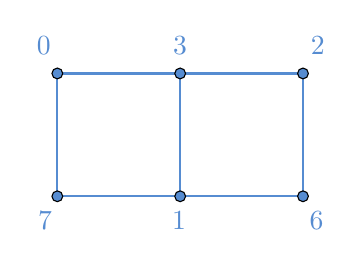
\begin{tikzpicture}[scale=0.78]
			\draw [cackithi,line width=0.8pt] (0.,2.)-- (4.,2.);
			\draw [cackithi,line width=0.8pt] (4.,2.)-- (4.,0.);
			\draw [cackithi,line width=0.8pt] (4.,0.)-- (0.,0.);
			\draw [cackithi,line width=0.8pt] (0.,0.)-- (0.,2.);
			\draw [cackithi,line width=0.8pt] (2.,2.)-- (2.,0.);
			
			\draw [fill=cackithi] (0.,2.) circle (2.5pt);
			\draw[color=cackithi] (-0.22,2.45) node {$0$};
			\draw [fill=cackithi] (4.,2.) circle (2.5pt);
			\draw[color=cackithi] (4.24,2.45) node {$2$};
			\draw [fill=cackithi] (4.,0.) circle (2.5pt);
			\draw[color=cackithi] (4.22,-0.4) node {$6$};
			\draw [fill=cackithi] (0.,0.) circle (2.5pt);
			\draw[color=cackithi] (-0.2,-0.4) node {$7$};
			\draw [fill=cackithi] (2.,2.) circle (2.5pt);
			\draw[color=cackithi] (2.,2.45) node {$3$};
			\draw [fill=cackithi] (2.,0.) circle (2.5pt);
			\draw[color=cackithi] (1.98,-0.4) node {$1$};
		\end{tikzpicture}
		
		\vspace*{-5pt}
		\caption{\small\textit{\color{cackithi}Hình được dán nhãn.}}
		\vspace*{-10pt}
	\end{figure}
	\begin{figure}[H]
		\vspace*{-10pt}
		\centering
		\captionsetup{labelformat= empty, justification=centering}
		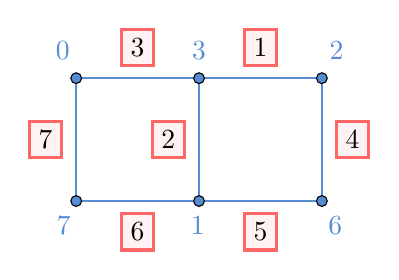
\begin{tikzpicture}[scale=0.78]
			\draw [cackithi,line width=0.8pt] (0.,2.)-- (4.,2.);
			\draw [cackithi,line width=0.8pt] (4.,2.)-- (4.,0.);
			\draw [cackithi,line width=0.8pt] (4.,0.)-- (0.,0.);
			\draw [cackithi,line width=0.8pt] (0.,0.)-- (0.,2.);
			\draw [cackithi,line width=0.8pt] (2.,2.)-- (2.,0.);
			
			\draw [fill=cackithi] (0.,2.) circle (2.5pt);
			\draw[color=cackithi] (-0.22,2.45) node {$0$};
			\draw(1,2.5) node[squarednode]{$3$};
			\draw [fill=cackithi] (4.,2.) circle (2.5pt);
			\draw[color=cackithi] (4.24,2.45) node {$2$};
			\draw(3,2.5) node[squarednode]{$1$};
			\draw [fill=cackithi] (4.,0.) circle (2.5pt);
			\draw[color=cackithi] (4.22,-0.4) node {$6$};
			\draw(3,-0.5) node[squarednode]{$5$};
			\draw(1,-0.5) node[squarednode]{$6$};
			\draw(-0.5,1) node[squarednode]{$7$};
			\draw(1.5,1) node[squarednode]{$2$};
			\draw(4.5,1) node[squarednode]{$4$};
			\draw [fill=cackithi] (0.,0.) circle (2.5pt);
			\draw[color=cackithi] (-0.2,-0.4) node {$7$};
			\draw [fill=cackithi] (2.,2.) circle (2.5pt);
			\draw[color=cackithi] (2.,2.45) node {$3$};
			\draw [fill=cackithi] (2.,0.) circle (2.5pt);
			\draw[color=cackithi] (1.98,-0.4) node {$1$};
		\end{tikzpicture}
		
		\vspace*{-5pt}
		\caption{\small\textit{\color{cackithi}Hình được dán nhãn và trọng số.}}
		\vspace*{-10pt}
	\end{figure}
	\textbf{\color{cackithi}A. Một vài ví dụ}
	\vskip 0.05cm
	$1.$ Trong các hình dưới đây, hình nào cho ta một dán nhãn duyên dáng ?
	\begin{figure}[H]
		\vspace*{-15pt}
		\centering
		\captionsetup{labelformat= empty, justification=centering}
		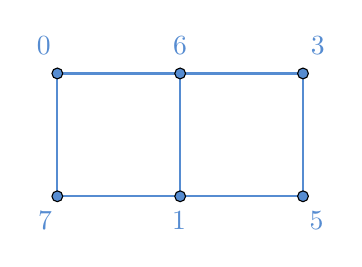
\begin{tikzpicture}[scale=0.78]
			\draw [cackithi,line width=0.8pt] (0.,2.)-- (4.,2.);
			\draw [cackithi,line width=0.8pt] (4.,2.)-- (4.,0.);
			\draw [cackithi,line width=0.8pt] (4.,0.)-- (0.,0.);
			\draw [cackithi,line width=0.8pt] (0.,0.)-- (0.,2.);
			\draw [cackithi,line width=0.8pt] (2.,2.)-- (2.,0.);
			
			\draw [fill=cackithi] (0.,2.) circle (2.5pt);
			\draw[color=cackithi] (-0.22,2.45) node {$0$};
			\draw [fill=cackithi] (4.,2.) circle (2.5pt);
			\draw[color=cackithi] (4.24,2.45) node {$3$};
			\draw [fill=cackithi] (4.,0.) circle (2.5pt);
			\draw[color=cackithi] (4.22,-0.4) node {$5$};
			\draw [fill=cackithi] (0.,0.) circle (2.5pt);
			\draw[color=cackithi] (-0.2,-0.4) node {$7$};
			\draw [fill=cackithi] (2.,2.) circle (2.5pt);
			\draw[color=cackithi] (2.,2.45) node {$6$};
			\draw [fill=cackithi] (2.,0.) circle (2.5pt);
			\draw[color=cackithi] (1.98,-0.4) node {$1$};
		\end{tikzpicture}
		\vspace*{-10pt}
	\end{figure}
	\begin{figure}[H]
		\vspace*{-15pt}
		\centering
		\captionsetup{labelformat= empty, justification=centering}
		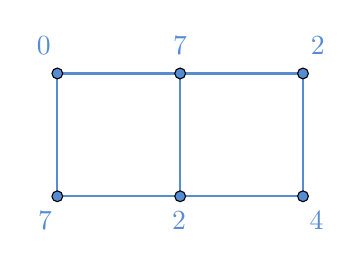
\begin{tikzpicture}[scale=0.78]
			\draw [cackithi, line width=0.8pt] (0.,2.)-- (4.,2.);
			\draw [cackithi,line width=0.8pt] (4.,2.)-- (4.,0.);
			\draw [cackithi,line width=0.8pt] (4.,0.)-- (0.,0.);
			\draw [cackithi,line width=0.8pt] (0.,0.)-- (0.,2.);
			\draw [cackithi,line width=0.8pt] (2.,2.)-- (2.,0.);
			
			\draw [fill=cackithi] (0.,2.) circle (2.5pt);
			\draw[color=cackithi] (-0.22,2.45) node {$0$};
			\draw [fill=cackithi] (4.,2.) circle (2.5pt);
			\draw[color=cackithi] (4.24,2.45) node {$2$};
			\draw [fill=cackithi] (4.,0.) circle (2.5pt);
			\draw[color=cackithi] (4.22,-0.4) node {$4$};
			\draw [fill=cackithi] (0.,0.) circle (2.5pt);
			\draw[color=cackithi] (-0.2,-0.4) node {$7$};
			\draw [fill=cackithi] (2.,2.) circle (2.5pt);
			\draw[color=cackithi] (2.,2.45) node {$7$};
			\draw [fill=cackithi] (2.,0.) circle (2.5pt);
			\draw[color=cackithi] (1.98,-0.4) node {$2$};
		\end{tikzpicture}
		\vspace*{-5pt}
	\end{figure}
	$2.$ Bổ sung hình sau để được một dán nhãn duyên dáng.
	\begin{figure}[H]
		\vspace*{-15pt}
		\centering
		\captionsetup{labelformat= empty, justification=centering}
		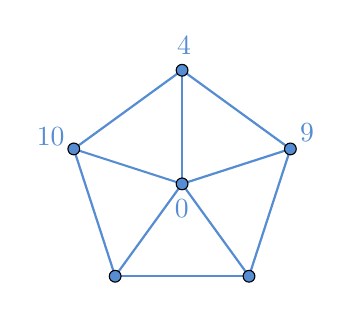
\begin{tikzpicture}[scale=0.85]
			\draw [cackithi,line width=0.75pt] (-1.6180339887498947,2.9021130325903073)-- (0.,2.38);
			\draw [cackithi,line width=0.8pt] (0.,2.38)-- (-1.,1.);
			\draw [cackithi,line width=0.8pt] (0.,2.38)-- (1.,1.);
			\draw [cackithi,line width=0.8pt] (0.,2.38)-- (1.618033988749895,2.9021130325903064);
			\draw [cackithi,line width=0.8pt] (0.,4.077683537175253)-- (0.,2.38);
			\draw [cackithi,line width=0.8pt] (0.,4.077683537175253)-- (-1.6180339887498947,2.9021130325903073);
			\draw [cackithi,line width=0.8pt] (-1.6180339887498947,2.9021130325903073)-- (-1.,1.);
			\draw [cackithi,line width=0.8pt] (-1.,1.)-- (1.,1.);
			\draw [cackithi,line width=0.8pt] (1.,1.)-- (1.618033988749895,2.9021130325903064);
			\draw [cackithi,line width=0.8pt] (1.618033988749895,2.9021130325903064)-- (0.,4.077683537175253);
			\draw [fill=cackithi] (-1.,1.) circle (2.5pt);
			%					\draw[color=cackithi] (-1.18624795654696,0.7809397247271022) node {$A$};
			\draw [fill=cackithi] (1.,1.) circle (2.5pt);
			%					\draw[color=cackithi] (1.209997363286399,0.7471897906449423) node {$B$};
			\draw [fill=cackithi] (1.618033988749895,2.9021130325903064) circle (2.5pt);
			\draw[color=cackithi] (1.8681210778885187,3.1434351104783014) node {$9$};
			\draw [fill=cackithi] (0.,4.077683537175253) circle (2.5pt);
			\draw[color=cackithi] (0.028749670410799504,4.4428075726414615) node {$4$};
			\draw [fill=cackithi] (-1.6180339887498947,2.9021130325903073) circle (2.5pt);
			\draw[color=cackithi] (-1.9624964404366394,3.0928102093550613) node {$10$};
			\draw [fill=cackithi] (0.,2.38) circle (2.5pt);
			\draw[color=cackithi] (-0.005000263671360479,2.012812318725942) node {$0$};
		\end{tikzpicture}
		\vspace*{-10pt}
	\end{figure}
	\textbf{\color{cackithi}B. Trường hợp thẳng hàng}
	\vskip 0.05cm
	Với mỗi số nguyên dương $n$, ta xét hình $L_n$ gồm $n+1$ điểm thẳng hàng và $n$ đoạn thẳng được tạo thành từ các điểm kề nhau.
	\vskip 0.05cm
	Ta đề xuất sự gán nhãn duyên dáng của những điểm của hình $L_4$ như sau :
	\begin{figure}[H]
		\vspace*{-10pt}
		\centering
		\captionsetup{labelformat= empty, justification=centering}
		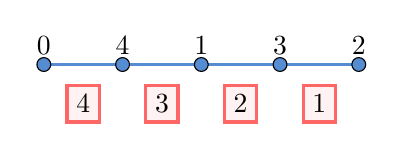
\begin{tikzpicture}
			\draw[cackithi, line width=0.8pt] (0,0) -- (4,0);
			\draw [fill=cackithi] (0,0) node[above]{$0$} circle (2.5pt);
			\draw [fill=cackithi] (1,0) node[above]{$4$} circle (2.5pt);
			\draw [fill=cackithi] (2,0) node[above]{$1$} circle (2.5pt);
			\draw [fill=cackithi] (3,0) node[above]{$3$} circle (2.5pt);
			\draw [fill=cackithi] (4,0) node[above]{$2$} circle (2.5pt);
			
			\draw(0.5,-0.5) node[squarednode]{$4$};
			\draw(1.5,-0.5) node[squarednode]{$3$};
			\draw(2.5,-0.5) node[squarednode]{$2$};
			\draw(3.5,-0.5) node[squarednode]{$1$};
		\end{tikzpicture}
		\vspace*{-10pt}
	\end{figure}
	$1.$ Chứng minh rằng tồn tại một dán nhãn duyên dáng cho mỗi hình $L_5,L_6$ và $L_7$.
	\vskip 0.05cm
	$2.$ Ta chấp nhận mà không chứng minh rằng tồn tại một dán nhãn duyên dáng đối với hình $L_{2022}$ sao cho điểm ngoài cùng bên trái được gắn số $0$. Hãy mô tả sự dán nhãn này. 
	\vskip 0.05cm
	\textbf{\color{cackithi}C. Trường hợp đa giác}
	\vskip 0.05cm
	$1.$ Chứng minh rằng mọi tam giác và tứ giác đều có thể được dán nhãn một cách duyên dáng. 
	\vskip 0.05cm
	$2.$ Dựa vào dán nhãn duyên dáng của hình đa giác $11$ cạnh dưới đây, hãy chỉ ra một cách dán nhãn duyên dáng của đa giác $12$ cạnh.
	\begin{figure}[H]
		\vspace*{-5pt}
		\centering
		\captionsetup{labelformat= empty, justification=centering}
		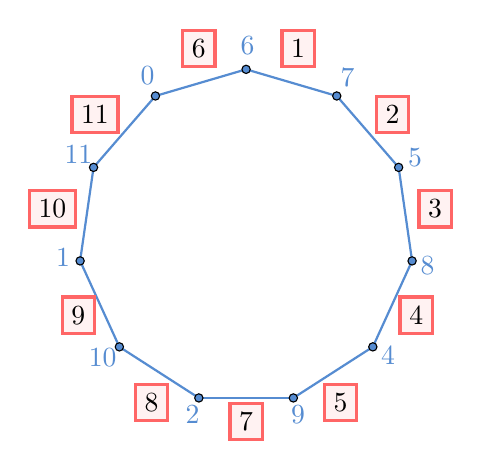
\begin{tikzpicture}[scale=0.6]
			\draw [cackithi, line width=0.8pt] (4.,0.)-- (6.,0.);
			\draw [cackithi,line width=0.8pt] (6.,0.)-- (7.682507065662361,1.0812816349111944);
			\draw [cackithi,line width=0.8pt] (7.682507065662361,1.0812816349111944)-- (8.513337091666134,2.90054562562023);
			\draw [cackithi,line width=0.8pt] (8.513337091666134,2.90054562562023)-- (8.228707415119565,4.880188509382095);
			\draw [cackithi,line width=0.8pt] (8.228707415119565,4.880188509382095)-- (6.918985947228994,6.3916876580906115);
			\draw [cackithi,line width=0.8pt] (6.918985947228994,6.3916876580906115)-- (5.,6.955152771773471);
			\draw [cackithi,line width=0.8pt] (5.,6.955152771773471)-- (3.081014052771007,6.391687658090612);
			\draw [cackithi,line width=0.8pt] (3.081014052771007,6.391687658090612)-- (1.7712925848804368,4.880188509382096);
			\draw [cackithi,line width=0.8pt] (1.7712925848804368,4.880188509382096)-- (1.4866629083338658,2.9005456256202327);
			\draw [cackithi,line width=0.8pt] (1.4866629083338658,2.9005456256202327)-- (2.317492934337639,1.0812816349111949);
			\draw [cackithi,line width=0.8pt] (2.317492934337639,1.0812816349111949)-- (4.,0.);
			
			\draw [fill=cackithi] (4.,0.) circle (2.5pt);
			\draw[color=cackithi] (3.868571428571432,-0.35) node {$2$};
			\draw(5,-0.5) node[squarednode]{$7$};
			\draw [fill=cackithi] (6.,0.) circle (2.5pt);
			\draw[color=cackithi] (6.09714285714286,-0.35) node {$9$};
			\draw(7,-0.1) node[squarednode]{$5$};
			\draw [fill=cackithi] (7.682507065662361,1.0812816349111944) circle (2.5pt);
			\draw[color=cackithi] (8.001904761904765,0.9009523809523803) node {$4$};
			\draw(8.6,1.75) node[squarednode]{$4$};
			\draw [fill=cackithi] (8.513337091666134,2.90054562562023) circle (2.5pt);
			\draw[color=cackithi] (8.84,2.8057142857142856) node {$8$};
			\draw(9,4) node[squarednode]{$3$};
			\draw [fill=cackithi] (8.228707415119565,4.880188509382095) circle (2.5pt);
			\draw[color=cackithi] (8.573333333333336,5.0914285714285725) node {$5$};
			\draw(8.1,6) node[squarednode]{$2$};
			\draw [fill=cackithi] (6.918985947228994,6.3916876580906115) circle (2.5pt);
			\draw[color=cackithi] (7.144761904761908,6.786666666666668) node {$7$};
			\draw(6.1,7.4) node[squarednode]{$1$};
			\draw [fill=cackithi] (5.,6.955152771773471) circle (2.5pt);
			\draw[color=cackithi] (5.030476190476193,7.453333333333335) node {$6$};
			\draw(4,7.4) node[squarednode]{$6$};
			\draw [fill=cackithi] (3.081014052771007,6.391687658090612) circle (2.5pt);
			\draw[color=cackithi] (2.9161904761904793,6.824761904761906) node {$0$};
			\draw(1.8,6) node[squarednode]{$11$};
			\draw [fill=cackithi] (1.7712925848804368,4.880188509382096) circle (2.5pt);
			\draw[color=cackithi] (1.4495238095238128,5.1485714285714295) node {$11$};
			\draw(0.9,4) node[squarednode]{$10$};
			\draw [fill=cackithi] (1.4866629083338658,2.9005456256202327) circle (2.5pt);
			\draw[color=cackithi] (1.125714285714289,2.977142857142857) node {$1$};
			\draw(1.45,1.75) node[squarednode]{$9$};
			\draw [fill=cackithi] (2.317492934337639,1.0812816349111949) circle (2.5pt);
			\draw[color=cackithi] (1.9638095238095272,0.8628571428571423) node {$10$};
			\draw(3,-0.1) node[squarednode]{$8$};
		\end{tikzpicture}
%		\vspace*{-5pt}
	\end{figure}
	$3.$ Xác định tính chẵn lẻ đối với trọng số của một đoạn thẳng khi mà các số được gán cho các đầu mút của nó: 
	\vskip 0.05cm
	$a.$ Khác nhau về tính chẵn lẻ.
	\vskip 0.01cm
	$b.$ Cùng tính chẵn lẻ. 
	\vskip 0.01cm
	$4.$ Từ đó suy ra rằng hình ngũ giác  không thể có dán nhãn duyên dáng. 
	\vskip 0.05cm
	\textbf{\color{cackithi}D. Một hình đa giác với số cạnh lớn}
	\vskip 0.05cm
	Ta ký hiệu $K_{2022}$ là hình được tạo thành từ $2022$ điểm sao cho mỗi cặp điểm bất kỳ trong chúng được nối với nhau bằng một đoạn thẳng duy nhất.
	\vskip 0.05cm
	$1.$ Chứng minh rằng $K_{2022}$ được tạo thành từ $2 043 231$ đoạn thẳng.
	\vskip 0.05cm
	$2.$ Giả sử rằng tồn tại một dán nhãn duyên dáng đối với hình $K_{2022}$.
	\vskip 0.05cm
	$a.$ Có bao nhiêu đoạn thẳng mang trọng số là số lẻ?
	\vskip 0.05cm
	$b.$ Ta ký hiệu $p$ là số điểm được dán nhãn là một số chẵn. Biểu diễn theo tham số $p$, số đoạn thẳng mà ở đó trọng số là một số lẻ.
	\vskip 0.05cm 
	$3.$ Chứng minh rằng hình $K_{2022}$ không thể có dán nhãn duyên dáng.
	\vskip 0.05cm
	\textbf{\color{cackithi}Bài $\pmb{2}$ (Dành cho thí sinh theo chương trình chuyên)}
	\vskip 0.05cm
	\textbf{\color{cackithi}Những số phân chia được}
	\vskip 0.05cm
	\textbf{\color{cackithi}Phần A}
	\vskip 0.05cm
	Ta nói rằng một số tự nhiên là \textit{phân chia được đơn nguyên} nếu như số đó lớn hơn hoặc bằng $3$ và viết được dưới dạng : $1+2+3+\cdots +p$, trong đó $p$ là một số tự nhiên lớn hơn hoặc bằng $2$. Ví dụ, $3$ và $10$ là những số tự nhiên phân chia được đơn nguyên bởi vì: $3 =1+2$  và $10=1+2+3+4$.
	\vskip 0.05cm 
	Ta nhắc lại rằng, tổng các số tự nhiên từ $1$ tới $n$ được cho bởi công thức:
	%	\setlength{\abovedisplayskip}{4pt}
	%	\setlength{\belowdisplayskip}{4pt} 
	\begin{align*}
		1+2+3+\cdots+n=\frac{n(n+1)}{2}.
	\end{align*}
	$1.$ $a.$ Chứng minh rằng $21$ và $136$ là những số tự nhiên phân chia được đơn nguyên.  
	\vskip 0.05cm
	$b.$ Số tự nhiên $1850$ có phân chia được đơn nguyên không?
	\vskip 0.05cm
	$2.$ Xét $a$ là một số tự nhiên lớn hơn hoặc bằng $3$. Hãy xác định điều kiện cần và đủ sao cho $a$ là một số tự nhiên phân chia được đơn~nguyên. 
	\vskip 0.05cm
	\textbf{\color{cackithi}Phần B}
	\vskip 0.05cm
	Ta nói rằng một số tự nhiên là phân chia được nếu nó có thể viết dưới dạng tổng của hai hoặc nhiều hơn các số nguyên dương liên tiếp. Ví dụ, $24$ và $25$ là những số tự nhiên phân chia được vì $24 = 7 + 8 + 9$ và $25 = 12 + 13$. Tuy nhiên $4$ không phải là số tự nhiên phân chia được vì $1 + 2 < 4 < 1 + 2 + 3$ và $2 + 3 > 4$.
	\vskip 0.05cm
	$1.$ Chứng minh rằng $9$ và $15$ là những số tự nhiên phân chia được nhưng $16$ thì không.
	\vskip 0.05cm
	$2.$ Chứng minh rằng mọi số nguyên lẻ lớn hơn hoặc bằng $3$ là phân chia được. 
	\vskip 0.05cm
	Xét $k$ và $q$ là những số tự nhiên với $k\ge 2$.  Đặt $S=(q+1)+(q+2)+\cdots+(q+k)$. Chứng minh rằng: $2S=k(k+1+2q)$.
	\vskip 0.05cm
	$4.$ Chứng minh rằng mọi lũy thừa của $2$ đều không phân chia được. 
	\vskip 0.05cm
	$5.$ Chúng ta quan tâm đến những số nguyên dương chẵn và không phải là lũy thừa của $2$. Gọi $n$ là một số như thế. Ta chấp nhận rằng tồn tại duy nhất một cặp số tự nhiên $(r,m)$ trong đó $m$ là một số tự nhiên lẻ lớn hơn hoặc bằng $3$ và $r$ một số tự nhiên lớn hơn hoặc bằng $1$, sao cho  $n=2^r\times m$.
	\vskip 0.05cm
	$a.$ Xác định $r$ và $m$ khi $n=56$. Từ đó chỉ ra rằng $56$ là một số phân chia được và hãy viết nó dưới dạng tổng của các số nguyên dương liên tiếp.
	\vskip 0.05cm
	$b.$ Chứng minh rằng $44$ là phân chia được.
	\vskip 0.05cm
	$c.$ Chứng minh rằng mọi  số nguyên dương chẵn và không phải là lũy thừa của $2$ là phân chia được. 
	\vskip 0.05cm
	$6.$ Từ những kết quả trên, hãy xác định tập hợp tất cả các số tự nhiên phân chia được.
	\vskip 0.05cm
	\textbf{\color{cackithi}Phần C}
	\vskip 0.05cm
	Một số tự nhiên được gọi là phân chia được một cách duy nhất nếu số đó được biểu diễn một cách duy nhất dưới dạng tổng của hai hoặc nhiều hơn các số nguyên dương liên tiếp.
	\vskip 0.05cm
	$1.$ Chứng minh rằng $13$ là số phân chia được một cách duy nhất. Số $25$ có phải là số phân chia được một cách duy nhất không?
	\vskip 0.05cm
	$2.$ $a.$ Xét số tự nhiên $n$ là tổng của k số tự nhiên dương liên tiếp, với $k\ ge3$. Ta có thể viết $n$ dưới dạng  $n=(q+1)+(q+2)+\cdots+(q+k)$, với $q$ là số tự nhiên. Chứng minh rằng $n$ không phải là số nguyên tố.
	\vskip 0.05cm
	$b$. Từ đó suy ra rằng mọi số nguyên tố lớn hơn hoặc bằng $3$ là phân chia được một cách duy nhất.
	\vskip 0.05cm
	\textbf{\color{cackithi}Bài $\pmb{3}$ (Dành cho các thí sinh không theo chương trình chuyên)}
	\vskip 0.05cm
	\textbf{\color{cackithi}Số ba}
	\vskip 0.05cm
	Ta xây dựng một dãy số tự nhiên dựa trên quy tắc sau.
	\vskip 0.05cm
	\textbf{\color{cackithi}Quy tắc}
	\vskip 0.05cm
	Số hạng đầu tiên của dãy là $4$.
	\vskip 0.05cm
	Từ một số hạng, để có số hạng tiếp theo, ta thực hiện một trong những phép toán sau:
	\vskip 0.05cm 
	$\bullet$ Nhân số đó với $3$;
	\vskip 0.05cm
	$\bullet$ Nhân số với $3$ rồi cộng kết quả nhận được với $2$;
	\vskip 0.05cm
	$\bullet$ Nếu là số chẵn thì chia cho $2$.
	\vskip 0.05cm
	Nếu một trong các dãy được xây dựng theo cách này có số hạng nào đó bằng $N$, thì ta nói rằng $N$ là \textit{số có thể đạt được}.
	\vskip 0.05cm 
	Ví dụ, số $11$ có thể đạt được: thật vậy, ta bắt đầu từ số $4$, nhân $4$ với $3$ để được $12$, sau đó ta chia $12$ cho $2$ hai lần liên tiếp để được $3$, sau đó nhân $3$ với $3$ rồi cộng $2$ ta được kết quả là $11$.
	\vskip 0.05cm 
	$1.$ Chứng tỏ rằng tất cả các số tự nhiên từ $1$ đến $12$ đều có thể đạt được bằng quy tắc nêu trên. 
	\vskip 0.05cm
	$2.$ Chứng tỏ rằng $2022$ có thể đạt được bằng quy tắc nêu trên. 
	\vskip 0.05cm
	$3.$ Giả sử rằng tồn tại các số tự nhiên không thể đạt được bằng cách áp dụng quy tắc nêu trên. Gọi $m$ là số nhỏ nhất như vậy.
	\vskip 0.05cm
	$a.$ Chứng tỏ rằng $m$ không phải là bội của $3$.
	\vskip 0.05cm
	$b.$ Chứng tỏ rằng $m-2$ không phải là bội của~$3$.
	\vskip 0.05cm
	$c.$ Chứng tỏ rằng $m-1$ cũng không phải là bội của $3$.
	\vskip 0.05cm
	$d.$ Dựa vào kết quả trên, hãy đưa ra kết luận. 
	\vskip 0.05cm
	\textbf{\color{cackithi}Lời giải}
	\vskip 0.05cm
	\textbf{\color{cackithi}Bài $\pmb{1}$ (Chung cho tất cả thí sinh).}
	\vskip 0.05cm
	\textbf{\color{cackithi}Sự dán nhãn duyên dáng của một hình.}
	\vskip 0.05cm
	\textbf{\color{cackithi}A.}
	$1.$ Hình thứ nhất không phải là một dán nhãn duyên dáng bởi vì có hai trọng số giống nhau: $6-0=6=7-1$. 
	%	\begin{figure}[H]
		%		\vspace*{-10pt}
		%		\centering
		%		\captionsetup{labelformat= empty, justification=centering}
		%		\begin{tikzpicture}
			%			\draw [cackithi,line width=0.8pt] (0.,2.)-- (4.,2.);
			%			\draw [cackithi,line width=0.8pt] (4.,2.)-- (4.,0.);
			%			\draw [cackithi,line width=0.8pt] (4.,0.)-- (0.,0.);
			%			\draw [cackithi,line width=0.8pt] (0.,0.)-- (0.,2.);
			%			\draw [cackithi,line width=0.8pt] (2.,2.)-- (2.,0.);
			%			
			%			\draw [fill=cackithi] (0.,2.) circle (2.5pt);
			%			\draw[color=cackithi] (-0.22,2.45) node {$0$};
			%			\draw [fill=cackithi] (4.,2.) circle (2.5pt);
			%			\draw[color=cackithi] (4.24,2.45) node {$3$};
			%			\draw [fill=cackithi] (4.,0.) circle (2.5pt);
			%			\draw[color=cackithi] (4.22,-0.4) node {$5$};
			%			\draw [fill=cackithi] (0.,0.) circle (2.5pt);
			%			\draw[color=cackithi] (-0.2,-0.4) node {$7$};
			%			\draw [fill=cackithi] (2.,2.) circle (2.5pt);
			%			\draw[color=cackithi] (2.,2.45) node {$6$};
			%			\draw [fill=cackithi] (2.,0.) circle (2.5pt);
			%			\draw[color=cackithi] (1.98,-0.4) node {$1$};
			%			\draw (1,2.5) node[squarednode] {$6$};
			%			\draw (1,-0.5) node[squarednode] {$6$};
			%		\end{tikzpicture}
		%		\vspace*{-5pt}
		%	\end{figure}
	Hình thứ hai cũng không phải là một dán nhãn duyên dáng bởi vì có hai nhãn $7$  bằng nhau. 
	%	\begin{figure}[H]
		%		\vspace*{-10pt}
		%		\centering
		%		\captionsetup{labelformat= empty, justification=centering}
		%		\begin{tikzpicture}
			%			\draw [cackithi, line width=0.8pt] (0.,2.)-- (4.,2.);
			%			\draw [cackithi,line width=0.8pt] (4.,2.)-- (4.,0.);
			%			\draw [cackithi,line width=0.8pt] (4.,0.)-- (0.,0.);
			%			\draw [cackithi,line width=0.8pt] (0.,0.)-- (0.,2.);
			%			\draw [cackithi,line width=0.8pt] (2.,2.)-- (2.,0.);
			%			
			%			\draw [fill=cackithi] (0.,2.) circle (2.5pt);
			%			\draw[color=cackithi] (-0.22,2.45) node {$0$};
			%			\draw [fill=cackithi] (4.,2.) circle (2.5pt);
			%			\draw[color=cackithi] (4.24,2.45) node {$7$};
			%			\draw [fill=cackithi] (4.,0.) circle (2.5pt);
			%			\draw[color=cackithi] (4.22,-0.4) node {$4$};
			%			\draw [fill=cackithi] (0.,0.) circle (2.5pt);
			%			\draw[color=cackithi] (-0.2,-0.4) node {$7$};
			%			\draw [fill=cackithi] (2.,2.) circle (2.5pt);
			%			\draw[color=cackithi] (2.,2.45) node {$7$};
			%			\draw [fill=cackithi] (2.,0.) circle (2.5pt);
			%			\draw[color=cackithi] (1.98,-0.4) node {$2$};
			%		\end{tikzpicture}
		%		\vspace*{-10pt}
		%	\end{figure}
	
	$2.$ Hình đã cho có thể được bổ sung như sau: 
	\begin{figure}[H]
		\vspace*{-10pt}
		\centering
		\captionsetup{labelformat= empty, justification=centering}
		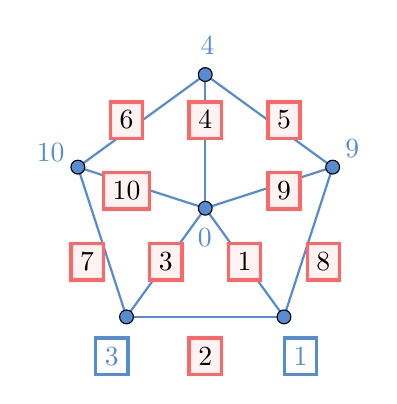
\begin{tikzpicture}
			\draw [cackithi,line width=0.8pt] (-1.6180339887498947,2.9021130325903073)-- (0.,2.38);
			\draw [cackithi,line width=0.8pt] (0.,2.38)-- (-1.,1.);
			\draw [cackithi,line width=0.8pt] (0.,2.38)-- (1.,1.);
			\draw [cackithi,line width=0.8pt] (0.,2.38)-- (1.618033988749895,2.9021130325903064);
			\draw [cackithi,line width=0.8pt] (0.,4.077683537175253)-- (0.,2.38);
			\draw [cackithi,line width=0.8pt] (0.,4.077683537175253)-- (-1.6180339887498947,2.9021130325903073);
			\draw [cackithi,line width=0.8pt] (-1.6180339887498947,2.9021130325903073)-- (-1.,1.);
			\draw [cackithi,line width=0.8pt] (-1.,1.)-- (1.,1.);
			\draw [cackithi,line width=0.8pt] (1.,1.)-- (1.618033988749895,2.9021130325903064);
			\draw [cackithi,line width=0.8pt] (1.618033988749895,2.9021130325903064)-- (0.,4.077683537175253);
			\draw [fill=cackithi] (-1.,1.) circle (2.5pt);
			\draw[color=cackithi] (-1.18624795654696,0.5) node[sqnode] {$3$};
			\draw (0,0.5) node[squarednode] {$2$};
			\draw (-1.5,1.7) node[squarednode] {$7$};
			\draw (-0.5,1.7) node[squarednode] {$3$};
			\draw (0.5,1.7) node[squarednode] {$1$};
			\draw (1.5,1.7) node[squarednode] {$8$};
			\draw (-1,3.5) node[squarednode] {$6$};
			\draw (-1,2.6) node[squarednode] {$10$};
			\draw (0,3.5) node[squarednode] {$4$};
			\draw (1,2.6) node[squarednode] {$9$};
			\draw (1,3.5) node[squarednode] {$5$};
			\draw [fill=cackithi] (1.,1.) circle (2.5pt);
			\draw[color=cackithi] (1.209997363286399,0.5) node[sqnode] {$1$};
			\draw [fill=cackithi] (1.618033988749895,2.9021130325903064) circle (2.5pt);
			\draw[color=cackithi] (1.8681210778885187,3.1434351104783014) node {$9$};
			\draw [fill=cackithi] (0.,4.077683537175253) circle (2.5pt);
			\draw[color=cackithi] (0.028749670410799504,4.4428075726414615) node {$4$};
			\draw [fill=cackithi] (-1.6180339887498947,2.9021130325903073) circle (2.5pt);
			\draw[color=cackithi] (-1.9624964404366394,3.0928102093550613) node {$10$};
			\draw [fill=cackithi] (0.,2.38) circle (2.5pt);
			\draw[color=cackithi] (-0.005000263671360479,2.012812318725942) node {$0$};
		\end{tikzpicture}
		%		\vspace*{-5pt}
	\end{figure}
	\textbf{\color{cackithi}B.} 	$1.$ Ví dụ về dán nhãn duyên dáng của $L_5, L_6, L_7$:
	%	
	%	Một dán nhãn duyên dáng của hình $L_5$	 
	%	
	\begin{figure}[H]
		\vspace*{-5pt}
		\centering
		\captionsetup{labelformat= empty, justification=centering}
		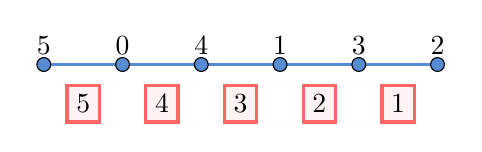
\begin{tikzpicture}
			\draw[cackithi, line width=0.8pt] (0,0) -- (5,0);
			\draw [fill=cackithi] (0,0) node[above]{$5$} circle (2.5pt);
			\draw [fill=cackithi] (1,0) node[above]{$0$} circle (2.5pt);
			\draw [fill=cackithi] (2,0) node[above]{$4$} circle (2.5pt);
			\draw [fill=cackithi] (3,0) node[above]{$1$} circle (2.5pt);
			\draw [fill=cackithi] (4,0) node[above]{$3$} circle (2.5pt);
			\draw [fill=cackithi] (5,0) node[above]{$2$} circle (2.5pt);
			
			
			\draw(0.5,-0.5) node[squarednode]{$5$};
			\draw(1.5,-0.5) node[squarednode]{$4$};
			\draw(2.5,-0.5) node[squarednode]{$3$};
			\draw(3.5,-0.5) node[squarednode]{$2$};
			\draw(4.5,-0.5) node[squarednode]{$1$};
		\end{tikzpicture}
		\vspace*{-10pt}
	\end{figure}
	%	Một dán nhãn duyên dáng của hình $L_6$	 
	\begin{figure}[H]
		\vspace*{-5pt}
		\centering
		\captionsetup{labelformat= empty, justification=centering}
		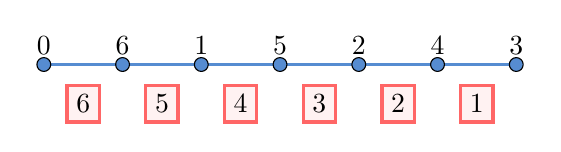
\begin{tikzpicture}
			\draw[cackithi, line width=0.8pt] (0,0) -- (6,0);
			\draw [fill=cackithi] (0,0) node[above]{$0$} circle (2.5pt);
			\draw [fill=cackithi] (1,0) node[above]{$6$} circle (2.5pt);
			\draw [fill=cackithi] (2,0) node[above]{$1$} circle (2.5pt);
			\draw [fill=cackithi] (3,0) node[above]{$5$} circle (2.5pt);
			\draw [fill=cackithi] (4,0) node[above]{$2$} circle (2.5pt);
			\draw [fill=cackithi] (5,0) node[above]{$4$} circle (2.5pt);
			\draw [fill=cackithi] (6,0) node[above]{$3$} circle (2.5pt);
			
			
			\draw(0.5,-0.5) node[squarednode]{$6$};
			\draw(1.5,-0.5) node[squarednode]{$5$};
			\draw(2.5,-0.5) node[squarednode]{$4$};
			\draw(3.5,-0.5) node[squarednode]{$3$};
			\draw(4.5,-0.5) node[squarednode]{$2$};
			\draw(5.5,-0.5) node[squarednode]{$1$};
		\end{tikzpicture}
		\vspace*{-10pt}
	\end{figure}
	%	Sự dán nhãn duyên dáng của hình $L_7$	 	
	\begin{figure}[H]
		\vspace*{-5pt}
		\centering
		\captionsetup{labelformat= empty, justification=centering}
		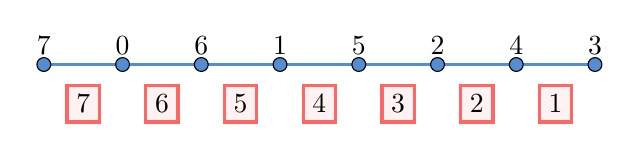
\begin{tikzpicture}
			\draw[cackithi, line width=0.8pt] (0,0) -- (7,0);
			\draw [fill=cackithi] (0,0) node[above]{$7$} circle (2.5pt);
			\draw [fill=cackithi] (1,0) node[above]{$0$} circle (2.5pt);
			\draw [fill=cackithi] (2,0) node[above]{$6$} circle (2.5pt);
			\draw [fill=cackithi] (3,0) node[above]{$1$} circle (2.5pt);
			\draw [fill=cackithi] (4,0) node[above]{$5$} circle (2.5pt);
			\draw [fill=cackithi] (5,0) node[above]{$2$} circle (2.5pt);
			\draw [fill=cackithi] (6,0) node[above]{$4$} circle (2.5pt);
			\draw [fill=cackithi] (7,0) node[above]{$3$} circle (2.5pt);
			
			
			\draw(0.5,-0.5) node[squarednode]{$7$};
			\draw(1.5,-0.5) node[squarednode]{$6$};
			\draw(2.5,-0.5) node[squarednode]{$5$};
			\draw(3.5,-0.5) node[squarednode]{$4$};
			\draw(4.5,-0.5) node[squarednode]{$3$};
			\draw(5.5,-0.5) node[squarednode]{$2$};
			\draw(6.5,-0.5) node[squarednode]{$1$};
		\end{tikzpicture}
		\vspace*{-10pt}
	\end{figure}
	$2.$ Tương tự như các dán nhãn đã nêu của $L_4$ và $L_6$, ta có thể dán nhãn hình $L_{2022}$ như sau: đánh số các điểm từ trái qua phải: 
	\begin{align*}
		&0,2022,1,2021,2,2020,3,2019,4,\\
		&2018 \ldots,1000,1012,1011
	\end{align*}
	Với cách dán nhãn trên, các trọng số từ trái qua phải là: $2022 ,$ $2021,$ $\ldots,4,3,2,1$. Đó là một dán nhãn duyên dáng của $L_{2022}$.
	\vskip 0.05cm 
	\textbf{\color{cackithi}C.} $1.$ Ví dụ cho tam giác và tứ giác: 
	\begin{figure}[H]
		\centering
		\vspace*{-5pt}
		\captionsetup{labelformat= empty, justification=centering}
		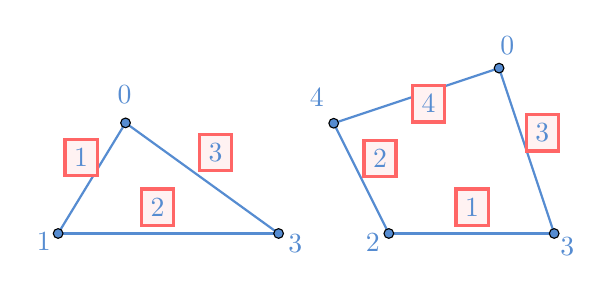
\begin{tikzpicture}[scale=0.7]
			\draw [cackithi, line width=0.8pt] (1.223091301970301,2.0066510197535226)-- (0,0);
			\draw [cackithi,line width=0.8pt] (0,0)-- (4,0);
			\draw [cackithi,line width=0.8pt] (4,0)-- (1.223091301970301,2.0066510197535226);
			\draw [cackithi,line width=0.8pt] (6,0)-- (5,2);
			\draw [cackithi,line width=0.8pt] (5,2)-- (8,3);
			\draw [cackithi,line width=0.8pt] (8,3)-- (9,0);
			\draw [cackithi,line width=0.8pt] (6,0)-- (9,0);
			
			\draw [fill=cackithi] (1.223091301970301,2.0066510197535226) circle (2.5pt);
			\draw[color=cackithi] (1.2043242804043022,2.522744112818487) node {$0$};
			\draw [fill=cackithi] (0,0) circle (2.5pt);
			\draw[color=cackithi] (-0.259503401743597,-0.14217294955332546) node {$1$};
			\draw[color=cackithi] (0.4161093746323564,1.3779557972925676) node[squarednode] {$1$};
			\draw [fill=cackithi] (4,0) circle (2.5pt);
			\draw[color=cackithi] (4.300882838794089,-0.17970699268532278) node {$3$};
			\draw[color=cackithi] (1.8048689705162608,0.4771387621246309) node[squarednode] {$2$};
			\draw[color=cackithi] (2.8558221782121884,1.4717909051225608) node[squarednode] {$3$};
			\draw [fill=cackithi] (6,0) circle (2.5pt);
			\draw[color=cackithi] (5.708409456243992,-0.16093997111932415) node {$2$};
			\draw [fill=cackithi] (5,2) circle (2.5pt);
			\draw[color=cackithi] (4.694990291680062,2.4664430481204906) node {$4$};
			\draw[color=cackithi] (5.839778607205983,1.3591887757265688) node[squarednode] {$2$};
			\draw [fill=cackithi] (8,3) circle (2.5pt);
			\draw[color=cackithi] (8.148122259823824,3.4047941264204247) node {$0$};
			\draw[color=cackithi] (6.721828620807923,2.3538409187244986) node[squarednode] {$4$};
			\draw [fill=cackithi] (9,0) circle (2.5pt);
			\draw[color=cackithi] (9.23660951065175,-0.23600805738331884) node {$3$};
			\draw[color=cackithi] (8.78620099306778,1.8283643148765356) node[squarednode] {$3$};
			\draw[color=cackithi] (7.510043526579868,0.4771387621246309) node[squarednode] {$1$};
		\end{tikzpicture}
		\vspace*{-10pt}
	\end{figure}
	$2.$ Thêm đỉnh số $12$ vào đa giác $11$ cạnh của bài ra như sau: 
	\begin{figure}[H]
		\centering
		%		\vspace*{-5pt}
		\captionsetup{labelformat= empty, justification=centering}
		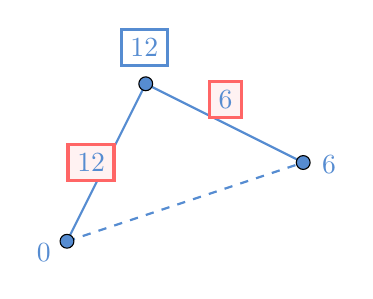
\begin{tikzpicture}
			\draw [cackithi, line width=0.8pt] (-3,3)-- (-4,1);
			\draw [cackithi,dashed, line width=0.8pt] (-4,1)-- (-1,2);
			\draw [cackithi,line width=0.8pt] (-3,3)-- (-1,2);
			
			\draw [fill=cackithi] (-3,3) circle (2.5pt);
			\draw[color=cackithi] (-3.018255571945407,3.4610951911184205) node[sqnode] {$12$};
			\draw [fill=cackithi] (-4,1) circle (2.5pt);
			\draw[color=cackithi] (-4.294413038433319,0.8524791934446044) node {$0$};
			\draw[color=cackithi] (-3.6938683483213604,2.0) node[squarednode] {$12$};
			\draw [fill=cackithi] (-1,2) circle (2.5pt);
			\draw[color=cackithi] (-0.6723778761955685,1.978500487404525) node {$6$};
			\draw[color=cackithi] (-1.986069385815478,2.8) node[squarednode] {$6$};
		\end{tikzpicture}
		\vspace*{-10pt}
	\end{figure}
	$3a.$ Lẻ. 
	\vskip 0.05cm
	$b.$  Chẵn.  
	\vskip 0.05cm
	$4.$ Giả sử ngược lại: tồn tại dán nhãn duyên dáng đối với hình ngũ giác. Khi đó trọng số các cạnh sẽ là các số tự nhiên từ $1$ tới $5$, do đó có $3$ số lẻ và $2$ số chẵn. Các đầu mút của $3$ cạnh có trọng số lẻ phải khác tính chẵn lẻ. Ta có hai trường hợp sau:
	\vskip 0.05cm 
	Trường hợp ${1}$: $3$ cạnh trọng số lẻ kề nhau.
	\begin{figure}[H]
		\centering
		\vspace*{-5pt}
		\captionsetup{labelformat= empty, justification=centering}
		\begin{tikzpicture}[scale=0.75]
			\draw [line width=0.8pt,color=cackithi] (-1,0)-- (1,0);
			\draw [line width=0.8pt,color=cackithi] (1,0)-- (1.618033988749895,1.9021130325903064);
			\draw [line width=0.8pt,color=cackithi] (1.618033988749895,1.9021130325903064)-- (0,3.077683537175253);
			\draw [line width=0.8pt,color=cackithi] (0,3.077683537175253)-- (-1.6180339887498947,1.9021130325903073);
			\draw [line width=0.8pt,color=cackithi] (-1.6180339887498947,1.9021130325903073)-- (-1,0);
			\draw [line width=0.8pt,color=cackithi] (4,0)-- (6,0);
			\draw [line width=0.8pt,color=cackithi] (6,0)-- (6.618033988749895,1.9021130325903064);
			\draw [line width=0.8pt,color=cackithi] (6.618033988749895,1.9021130325903064)-- (5,3.077683537175253);
			\draw [line width=0.8pt,color=cackithi] (5,3.077683537175253)-- (3.381966011250105,1.9021130325903073);
			\draw [line width=0.8pt,color=cackithi] (3.381966011250105,1.9021130325903073)-- (4,0);
			
			\draw [fill=cackithi] (-1,0) circle (2.5pt);
			\draw[color=cackithi] (-1.291689587873526,-0.6) node[squarednode] {L};
			\draw(0,0)node[below] {Chẵn};
			\draw [fill=cackithi] (1,0) circle (2.5pt);
			\draw[color=cackithi] (1.2418583235362997,-0.6) node[squarednode] {L};
			\draw(1.5,1)node[below] {Lẻ};
			\draw [fill=cackithi] (1.618033988749895,1.9021130325903064) circle (2.5pt);
			\draw[color=cackithi] (1.9,1.3) node[squarednode] {C};
			\draw(1,3)node[below] {Lẻ};
			\draw [fill=cackithi] (0,3.077683537175253) circle (2.5pt);
			\draw[color=cackithi] (0.022001921746383594,3.7) node[squarednode] {L};
			\draw(-1,3)node[below] {Lẻ};
			\draw [fill=cackithi] (-1.6180339887498947,1.9021130325903073) circle (2.5pt);
			\draw[color=cackithi] (-1.929768321117482,2.5) node[squarednode] {C};
			\draw(-1.3,1)node[below] {Chẵn};
			\draw [fill=cackithi] (4,0) circle (2.5pt);
			\draw[color=cackithi] (3.85047432121012,-0.6) node[squarednode] {C};
			\draw(5,0)node[below] {Chẵn};
			\draw(6.6,0.9)node[below] {Lẻ};
			\draw(6,3)node[below] {Lẻ};
			\draw(4,3)node[below] {Lẻ};
			\draw(3,1)node[below] {Chẵn};
			\draw [fill=cackithi] (6,0) circle (2.5pt);
			\draw[color=cackithi] (6.140050952261962,-0.6) node[squarednode] {C};
			\draw [fill=cackithi] (6.618033988749895,1.9021130325903064) circle (2.5pt);
			\draw[color=cackithi] (6.909498836467909,1.2224717677625083) node[squarednode] {L};
			\draw [fill=cackithi] (5,3.077683537175253) circle (2.5pt);
			\draw[color=cackithi] (5.032796679868039,3.7) node[squarednode] {C};
			\draw [fill=cackithi] (3.381966011250105,1.9021130325903073) circle (2.5pt);
			\draw[color=cackithi] (3.081026437004173,2.5) node[squarednode] {L};
		\end{tikzpicture}
		\vspace*{-10pt}
	\end{figure}
	Trường hợp ${2}$: $2$ cạnh trọng số lẻ kề nhau liền kề với một cạnh có trọng số chẵn. 
	\begin{figure}[H]
		\centering
		\vspace*{5pt}
		\captionsetup{labelformat= empty, justification=centering}
		\begin{tikzpicture}[scale=0.75]
			\draw [line width=0.8pt,color=cackithi] (-1,0)-- (1,0);
			\draw [line width=0.8pt,color=cackithi] (1,0)-- (1.618033988749895,1.9021130325903064);
			\draw [line width=0.8pt,color=cackithi] (1.618033988749895,1.9021130325903064)-- (0,3.077683537175253);
			\draw [line width=0.8pt,color=cackithi] (0,3.077683537175253)-- (-1.6180339887498947,1.9021130325903073);
			\draw [line width=0.8pt,color=cackithi] (-1.6180339887498947,1.9021130325903073)-- (-1,0);
			\draw [line width=0.8pt,color=cackithi] (4,0)-- (6,0);
			\draw [line width=0.8pt,color=cackithi] (6,0)-- (6.618033988749895,1.9021130325903064);
			\draw [line width=0.8pt,color=cackithi] (6.618033988749895,1.9021130325903064)-- (5,3.077683537175253);
			\draw [line width=0.8pt,color=cackithi] (5,3.077683537175253)-- (3.381966011250105,1.9021130325903073);
			\draw [line width=0.8pt,color=cackithi] (3.381966011250105,1.9021130325903073)-- (4,0);
			
			\draw [fill=cackithi] (-1,0) circle (2.5pt);
			\draw[color=cackithi] (-1.291689587873526,-0.6) node[squarednode] {C};
			\draw(0,0)node[below] {Lẻ};
			\draw [fill=cackithi] (1,0) circle (2.5pt);
			\draw[color=cackithi] (1.2418583235362997,-0.6) node[squarednode] {L};
			\draw(1.5,1)node[below] {Chẵn};
			\draw [fill=cackithi] (1.618033988749895,1.9021130325903064) circle (2.5pt);
			\draw[color=cackithi] (1.9,1.3) node[squarednode] {L};
			\draw(1,3)node[below] {Lẻ};
			\draw [fill=cackithi] (0,3.077683537175253) circle (2.5pt);
			\draw[color=cackithi] (0.022001921746383594,3.7) node[squarednode] {C};
			\draw(-1,3)node[below] {Lẻ};
			\draw [fill=cackithi] (-1.6180339887498947,1.9021130325903073) circle (2.5pt);
			\draw[color=cackithi] (-1.929768321117482,2.5) node[squarednode] {L};
			\draw(-1.3,1)node[below] {Chẵn};
			\draw [fill=cackithi] (4,0) circle (2.5pt);
			\draw[color=cackithi] (3.85047432121012,-0.6) node[squarednode] {L};
			\draw(5,0)node[below] {Lẻ};
			\draw(6.6,0.9)node[below] {Chẵn};
			\draw(6,3)node[below] {Lẻ};
			\draw(4,3)node[below] {Lẻ};
			\draw(3,1)node[below] {Chẵn};
			\draw [fill=cackithi] (6,0) circle (2.5pt);
			\draw[color=cackithi] (6.140050952261962,-0.6) node[squarednode] {C};
			\draw [fill=cackithi] (6.618033988749895,1.9021130325903064) circle (2.5pt);
			\draw[color=cackithi] (6.909498836467909,1.2224717677625083) node[squarednode] {C};
			\draw [fill=cackithi] (5,3.077683537175253) circle (2.5pt);
			\draw[color=cackithi] (5.032796679868039,3.7) node[squarednode] {L};
			\draw [fill=cackithi] (3.381966011250105,1.9021130325903073) circle (2.5pt);
			\draw[color=cackithi] (3.081026437004173,2.5) node[squarednode] {C};
		\end{tikzpicture}
		\vspace*{-15pt}
	\end{figure}
	Trong mọi trường hợp, tồn tại hai đỉnh liên tiếp, khác tính chẵn lẻ nhưng lại cho trọng số chẵn như minh họa phía trên, mâu thuẫn. 	\vskip 0.05cm 
	\textbf{\color{cackithi}D. }	$1.$ Hình $K_{2022}$ có  $C^2_{2022}=\dfrac{1}{2}\times 2022\times 2021=2043231$ đoạn thẳng. 
	\vskip 0.05cm
	$2a.$ Có $1021616$ đoạn thẳng có trọng số \linebreak lẻ là.
	\vskip 0.05cm 
	$b.$ Có $p$ điểm được dán nhãn chẵn và  $2022-p$ điểm được dán nhãn lẻ. Số các đoạn thẳng có trọng số lẻ chính là số cặp điểm được dán nhãn khác tính chẵn lẻ, nghĩa là $p(2022-p)$.
	\vskip 0.05cm
	$3.$ Giả sử ngược lại, khi đó số các đoạn thẳng có trọng số lẻ là $1021616$, vì thế tồn tại một số tự nhiên $p$ sao cho $p(2022-p)=1 021 616$. Nhưng phương trình này không có nghiệm nguyên, mâu thuẫn. 
	\vskip 0.05cm
	\textbf{\color{cackithi}Bài $\pmb{2}$} 
	\vskip 0.05cm
	\textbf{\color{cackithi} A.} $1a$. Các số $21$ và $136$ là phân chia được đơn nguyên vì: $21=1+2 + \cdots +6$ và $136=1+2+\cdots + 16$.
	\vskip 0.05cm 
	$b.$ Giả sử $1850$ là phân chia được đơn nguyên. Khi đó tồn tại số tự nhiên $n$ sao cho: 
	$1+2+\cdots+n=1850$,
	%	\end{align*}
%	Suy ra 
%	\begin{align*}
%		\frac{n(n+1)}{2} = 1850.
%	\end{align*}
dẫn đến $n^2+n-3700=0$. Nhưng phương trình bậc hai này không có nghiệm nguyên, mâu thuẫn. 

\vskip 0.05cm
$2.$ Số tự nhiên $a\ge 3$ là một số phân chia được đơn nguyên khi và chỉ khi phương trình: $n^2+n-2a=0$ có ít nhất một nghiệm nguyên dương. Từ đó dễ thấy điều kiện cần và đủ là $1+8a$ là số chính phương.
\vskip 0.05cm  
\textbf{\color{cackithi} B.}
$1.$ Các số $9$ và $15$ là phân chia được vì $9=4+5$ và $15=7+8$. Tuy nhiên, $16$ không phân chia được vì:
\begin{align*}
&1\!+\!2\!+\!3\!+\!4\!+\!5\!<\!16\!<\!1\!+\!2\!+\!3\!+\!4\!+\!5\!+\!6;\\
&2+3+4+5<16<2+3+4+5+6;\\
&3+4+5<16<3+4+5+6;\\
&4+5+6<16<4+5+6+7;\\
&5\!+\!6\!<\!16\!<\!5\!+\!6\!+\!7; 6\!+\!7\!<\!16\!<\!6\!+\!7\!+\!8;\\
&7+8<16<7+8+9 \text{ và } 8+9>16.
\end{align*}
$2.$ Đặt $n=2k+1$. Khi đó $n=k+(k+1)$, do đó là phân chia được.
\vskip 0.05cm  
$3.$ Hiển nhiên.
\vskip 0.05cm
$4.$ Giả sử $N=2^p$ là phân chia được. Theo câu trên, tồn tại các số nguyên $k, q\ge 2$ sao cho: $2^{p+1}=k(2q+k+1)$. Điều này là vô lý vì vế trái là một luỹ thừa của $2$ còn vế phải là tích của một số chẵn và một số lẻ lớn hơn $1$. 
\vskip 0.05cm
$5a.$ Ta có $56=2^3\times7$ nên $r=3$ và $m=7$. Do đó $2\times 56=2^4\times7=7(2\times 4+7+1)$ vì thể $56$ là phân chia được theo câu $B.3$. Cụ thể hơn, $56=5+6+ \cdots + 11$. 
\vskip 0.05cm
$b.$ Tương tự, $2\times 44=8\times11=8(2\times1+8+1)$. Do đó $44=2+3+\cdots + 9$ và $44$ là phân chia được.
\vskip 0.05cm 
$c.$  Đặt $n=2^r\times m$, với $m\ge 3$ là một số nguyên lẻ  và $r$ nguyên dương. Ta suy ra $2n=2^{r+1}\times m$.  Xét hai trường hợp sau. 
\vskip 0.05cm
Trường hợp $1$: $m>2^{r+1}$. Tồn tại số tự nhiên $l$ sao cho $m=2^{r+1}+1+2l$. Khi đó $2n=2^{r+1}(2l+2^{r+1}+1)$, vì thế theo câu $B.3$ thì $n$ phân chia được. 
\vskip 0.05cm
Trường hợp $2$: $m<2^{r+1}$. Tồn tại một số tự nhiên $l$ sao cho $2^{r+1}=m+1+2l$. Khi đó $2n=m(2l+m+1)$ Vì thế, vẫn theo câu $B.3$ thì $n$ phân chia được.  
\vskip 0.05cm
$6.$ Từ các câu $2$ và $5$, ta suy ra rằng tập hợp những số tự nhiên phân chia được là những số tự nhiên lẻ lớn hơn hoặc bằng $3$ và những số tự nhiên chẵn không phải là lũy thừa của $2$. 
\vskip 0.05cm
\textbf{\color{cackithi} C.}
$1.$ Do $13$ là số tự nhiên lẻ lớn hơn $3$, nên theo phần trên là phân chia được. Cụ thể, $13=6+7$. Đây là biểu diễn duy nhất của $13$. Thật vậy, nếu $13=(q'+1)+(q'+2)+\cdots+(q'+k')$ với $k'\ge 2$ và $q' $. Khi đó $2\times 13=k'(2q'+k'+1)$. Vì $2q'+k'+1>k'$ nên ta suy ra $k'<13$. Vì $13$ là số nguyên tố, nên ta suy ra $k'$ là ước của $2$, chứng tỏ $k'$. Từ đó $q'=5$ và ta nhận được biểu diễn $13=6+7$. Vậy, $13$ là số phân chia được một cách duy nhất. 
\vskip 0.05cm
Số $25$ là phân chia được, nhưng không phải là phân chia được một cách duy nhất do $25=12+13=3+4+5+6+7$.
\vskip 0.05cm 
$2a.$ Ta có $n=(q+1)+(q+2)+\cdots+(q+k)$, hay $n=\dfrac{k(2q+k+1)}{2}$. Tùy vào tính chẵn lẻ của $k$, một trong hai biểu diễn $n= \dfrac{k}{2}\cdot (2q+k+1)$, $n =k\cdot \dfrac{2q+ k+1}{2}$ cho thấy $n$ là tích của hai số nguyên $>1$, do đó là không là số nguyên tố. 

\vskip 0.05cm 
$b$. Giả sử $p$ là một số nguyên tố $\ge 3$. Theo phần $B$, ta biết rằng $p$ là phân chia được. Cụ thể, $p=(q+1)+(q+2)$ với $q=\dfrac{p-3}{2}$. Ta sẽ chứng minh biểu diễn này là duy nhất. Giả sử $p=(q'+1)+(q'+2)+\cdots+(q'+k')$ với các số tự nhiên $q'$ và $k'\ge 2$. Suy ra $2 p=k'(2q'+k'+1)$. Vì $2q'+k'+1>k'$ nên $k'<p$ là một ước $\ge 2$ nhưng $<p$ của $2p$. Mà các ước của $2p$ là $1, 2, p, 2p$ nên ta suy ra $k'=2$. Từ đó $q'=q$. Vậy, mọi số nguyên tố lớn hơn hoặc bằng $3$ đều phân chia được một cách duy nhất. 
\vskip 0.05cm
\textbf{\color{cackithi}Bài $\pmb{3}$} 
\vskip 0.05cm
$1.$ Tất cả các số tự nhiên từ $1$ đến $12$ đều có thể đạt được bằng các quy tắc của đề bài, chẳng hạn:
\vskip 0.05cm
\begin{tikzcd}[column sep = 1.35em]
4 \arrow{r}{:\ 2}  & 2 \arrow{r}{:\ 2}& 1, &4 \arrow{r}{:\ 2}  & 2,\\[-2.2ex]
4 \arrow{r}{:\ 2}  & 2 \arrow{r}{\times 3}& 6  \arrow{r}{:\  2} & 3, & 4,\\[-2.2ex]
4 \arrow{r}{:\ 2}  & 2 \arrow{r}{:\ 2} &1 \arrow{r}{\times 3}& 3  \arrow{r}{+2} & 5,\\[-2.2ex]
4 \arrow{r}{:\ 2}  & 2 \arrow{r}{\times 3}& 6,\\[-2.2ex]
4 \arrow{r}{\times  3}  & 12 \arrow{r}{+ 2}& 14\arrow{r}{: \ 2 }& 7,
\end{tikzcd}

\begin{tikzcd}[column sep = 1.35em]
	4 \arrow{r}{:\  2}  & 2 \arrow{r}{\times 3}& 6 \arrow{r}{+2 }& 8, \\[-2.2ex]
4 \arrow{r}{:\ 2}  & 2 \arrow{r}{:\ 2} &1 \arrow{r}{\times 3}& 3  \arrow{r}{\times 3} & 9, \\[-2.2ex]
4 \arrow{r}{:\ 2}  & 2 \arrow{r}{\times 3} &6 \arrow{r}{\times 3}& 18  \arrow{r}{+ 2} & 20 \arrow{r}{:\ 2} & 10,\\[-2.2ex]
4 \arrow{r}{:\ 2}  & 2 \arrow{r}{:\ 2} &1 \arrow{r}{\times 3}& 3  \arrow{r}{\times 3} & 9 \arrow{r}{+ 2} & 11,\\[-2.2ex]
4  \arrow{r}{\times 3} &12.
\end{tikzcd}
\vskip 0.1cm
$2.$ Ta có thể đạt được $2022$ như sau: trước hết, dựa vào câu $1$, ta có thể thu được $8$, sau đó:
\[
\begin{tikzcd}[column sep = 1.35em]
8 \arrow{r}{\times 3} & 24\arrow{r}{\times 3} & 72 \arrow{r}{+ 2} & 74 \arrow{r}{\times 3}& 222\\[-2.2ex]
222 \arrow{r}{+ 2} & 224 \arrow{r}{\times 3} & 672 \arrow{r}{+ 2} & 674 \arrow{r}{\times 3} & 2022.
\end{tikzcd}
\]
$3a$. Giả sử $m=3a$, với $a$ là số tự nhiên. Do $a<m$ nên $a$ là số đạt được. Thế nhưng khi đó, sau khi đạt được $a$, ta chỉ cần Nhân 3  để đạt được $m$. Chứng tỏ $m$ cũng đạt được, mâu thuẫn. 
\vskip 0.05cm 
$b$. Giả sử $m-2=3b$. Do $b<m$ nên $b$ là đạt được. Khi đó, sau khi đạt được $b$, ta chỉ cần áp dụng thêm $2$ phép toán:  Nhân $3$, sau đó Cộng $2$,  để thu được $m$. Vậy, $m$ cũng đạt được, mâu thuẫn. 
\vskip 0.05cm
$c.$ Giả sử $m-1=3c$. Ta có $m=3c+1>2c$ nên $2c$ cũng đạt được. Khi đó, sau khi đạt được $2c$, ta lần lượt thực hiện các phép toán  Nhân $3$,  Cộng $2$,  rồi  Chia $2$, ta thu được $m$. Vậy, $m$ cũng đạt được, mâu thuẫn. 
\vskip 0.05cm
$d.$ Từ các lập luận ở trên, ta thấy rằng không có số nguyên dương không đạt được nhỏ nhất. Chứng tỏ không có số nguyên dương không đạt được, hay, mọi số nguyên dương đều đạt được.
\vskip 0.05cm
\textbf{\color{cackithi}\color{cackithi}Tài liệu tham khảo}
\vskip 0.05cm
[$1$]  Tạp chí Pi, tập $6$, số $7-8$, năm $2022$.
\vskip 0.05cm

[$2$] Les Olympiades nationales de mathématiques | Ministère de l'Education Nationale et de la Jeunesse.
\vskip 0.05cm
[$3$] {\color{cackithi}https://www.freemaths.fr/annales-olym\\piades-mathematiques-premieres-scientifiqu\\es-s/nationales/2022}
\end{multicols}


%	 \newpage
	 
	 \setcounter{figure}{0}
	 \thispagestyle{lichsutoanhocnone}
\pagestyle{lichsutoanhoc}
\graphicspath{{../lichsutoanhoc/pic/}}
\everymath{\color{lichsutoanhoc}}
\blfootnote{$^1$\color{lichsutoanhoc}Cộng tác viên Viện Toán học.}
\begingroup
\AddToShipoutPicture*{\put(0,616){\includegraphics[width=19.3cm]{../bannerlichsu}}}
\AddToShipoutPicture*{\put(58,442){\includegraphics[scale=1]{../tieude.pdf}}}
\centering
\endgroup

\vspace*{263pt}

\begin{multicols}{2}
	\setlength{\abovedisplayskip}{5pt}
	\setlength{\belowdisplayskip}{5pt}
	$\pmb{1.}$ \textbf{\color{lichsutoanhoc}Số vô tỷ}
	\vskip 0.05cm
	Hippasus xứ Croton, khoảng $530-450$ trước công nguyên (TCN), ban đầu là người thuộc trường phái Pythagoras, nhưng sau bị khai trừ khỏi trường phái này. Một tài liệu nói những người Pythagoras đã dựng bia mộ ông, như thể ông đã chết; một tài liệu khác nói rằng sự bội đạo của ông đã bị trừng phạt bằng cái chết trên biển trong một tai nạn chìm tàu. Nguyên nhân chính xác có lẽ không bao giờ được biết, do quy tắc bí mật của trường phái Pythagoras, nhưng có ba khả năng đã được nêu ra. 
	\vskip 0.05cm
	Khả năng thứ nhất, Hippasus bị trục xuất vì ông đứng đầu một phong trào dân chủ chống lại những quy định bảo thủ của Pythagoras.
	\vskip 0.05cm
	Khả năng thứ hai quy việc trục xuất ông về lý do ông đã tiết lộ các phát minh của trường phái Pythagoras về ngũ giác đều hoặc khối $12$ mặt đều. 
	\vskip 0.05cm
	Giải thích thứ ba cho rằng ông bị trục xuất vì tiết lộ một khám phá toán học có ý nghĩa tàn khốc đối với học thuyết Pythagoras -- sự tồn tại các số vô tỷ.
	\vskip 0.1cm
	Nguyên lý cơ bản của học thuyết Pythagoras là các thuộc tính của số nguyên hoặc tỷ lệ của chúng (các số hữu tỷ) có thể giải thích bản chất của tất cả mọi thứ, trong hình học cũng như trong thiên văn và xã hội. Tuy nhiên, \textit{Đối thoại} của Plato (khoảng $428-347$ TCN) cho thấy rằng cộng đồng toán học Hy Lạp đã bị choáng váng bởi một tiết lộ hầu như phá hủy toàn bộ niềm tin của người Pythagoras và cộng đồng vào những con số. Đây là khám phá rằng trong bản  thân hình học, các số hữu tỷ không đủ để giải thích các thuộc tính cơ bản. Chẳng hạn, số hữu tỷ không đủ để so sánh tỷ lệ của đường chéo hình vuông, đường chéo hình lập phương hoặc đường chéo ngũ giác đều với cạnh của nó. 
	\vskip 0.1cm
	Thông thường, người ta cho rằng sự công nhận số vô tỷ liên quan đến ứng dụng của định lý Pythagoras vào tam giác vuông cân. Một chứng minh như vậy rất dễ xây dựng (xem [$10$]). Aristotle ($384-322$ TCN) đã đề cập đến một chứng minh về tính không thông ước\footnote[2]{\color{lichsutoanhoc}Hai đoạn thẳng có độ dài $a$ và $b$ được gọi là thông ước với nhau nếu tồn tại một đoạn thẳng có độ dài $c$ và các số tự nhiên $m$ và $n$ sao cho $a = mc$ và $b = nc$, tức là $\frac{a}{b} = \frac{m}{n}$. Theo ngôn ngữ ngày nay, hai đại lượng là thông ước nếu thương của chúng là một số hữu tỷ.} của đường chéo của hình vuông với cạnh của nó. Trong chứng minh này, mức độ trừu tượng cao đến mức người ta nghi ngờ nó đã được thực hiện vào thế kỉ V TCN. Tuy nhiên,  khám phá về số vô tỷ có thể đã xảy ra vào thế kỉ V TCN theo những cách khác. 
	\vskip 0.1cm
	Năm đường chéo của một ngũ giác đều tạo thành một ngũ giác đều nhỏ hơn và các đường chéo của hình ngũ giác thứ hai lần lượt tạo thành hình ngũ giác đều thứ ba ... (Hình $1$).
	\begin{figure}[H]
		\vspace*{-10pt}
		\centering
		\captionsetup{labelformat= empty, justification=centering}
		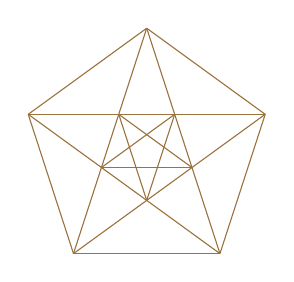
\begin{tikzpicture}[lichsutoanhoc,scale=0.62]
			\draw  (-1.,1.)-- (2.,1.);
			\draw  (2.,1.)-- (2.9270509831248424,3.85316954888546);
			\draw  (2.9270509831248424,3.85316954888546)-- (0.5,5.616525305762879);
			\draw  (0.5,5.616525305762879)-- (-1.927050983124842,3.853169548885461);
			\draw  (-1.927050983124842,3.853169548885461)-- (-1.,1.);
			\draw  (0.5,5.616525305762879)-- (2.,1.);
			\draw  (0.5,5.616525305762879)-- (-1.,1.);
			\draw  (-1.927050983124842,3.853169548885461)-- (2.9270509831248424,3.85316954888546);
			\draw  (2.9270509831248424,3.85316954888546)-- (-1.,1.);
			\draw  (-1.927050983124842,3.853169548885461)-- (2.,1.);
			\draw  (-0.07294901687515731,3.85316954888546)-- (1.4270509831248426,2.763355756877419);
			\draw  (-0.07294901687515731,3.85316954888546)-- (0.5,2.0898137920080413);
			\draw  (0.5,2.0898137920080413)-- (1.0729490168751583,3.853169548885459);
			\draw  (1.0729490168751583,3.853169548885459)-- (-0.4270509831248419,2.763355756877419);
			\draw  (-0.4270509831248419,2.763355756877419)-- (1.4270509831248426,2.763355756877419);
		\end{tikzpicture}
		\caption{\small\textit{\color{lichsutoanhoc}Hình $1$.}}
		\vspace*{-10pt}
	\end{figure}
	Quá trình này có thể được tiếp tục đến vô hạn, dẫn đến gợi ý: \textit{Tỷ số giữa một đường chéo và một cạnh của một ngũ giác đều không thể là số hữu tỷ.} 
	\vskip 0.1cm
	Xét ngũ giác đều $ABCDE$  với hai đường chéo $AD$  và $BE$  (Hình $2$). Do $\angle ABE = \angle IAE$ và $\angle AEB = \angle IEA$  nên $\Delta ABE \sim \Delta IAE$.  
	\begin{figure}[H]
		\vspace*{-10pt}
		\centering
		\captionsetup{labelformat= empty, justification=centering}
		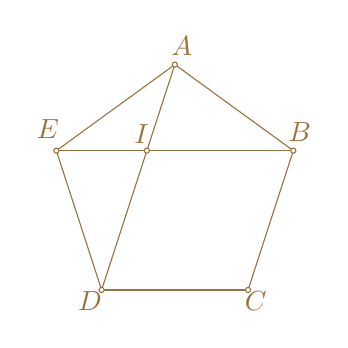
\begin{tikzpicture}[lichsutoanhoc,scale=0.62]
			\draw  (1.5,4.616525305762879)-- (3.9270509831248424,2.85316954888546);
			\draw  (3.9270509831248424,2.85316954888546)-- (3.,0.);
			\draw  (3.,0.)-- (0.,0.);
			\draw  (0.,0.)-- (-0.9270509831248419,2.853169548885461);
			\draw  (-0.9270509831248419,2.853169548885461)-- (1.5,4.616525305762879);
			\draw  (-0.9270509831248419,2.853169548885461)-- (3.9270509831248424,2.85316954888546);
			\draw  (1.5,4.616525305762879)-- (0.,0.);
	
				\draw [fill=white] (0.,0.) circle (1.5pt);
				\draw (-0.24,-0.23) node {$D$};
				\draw [fill=white] (3.,0.) circle (1.5pt);
				\draw (3.16,-0.23) node {$C$};
				\draw [fill=white] (3.9270509831248424,2.85316954888546) circle (1.5pt);
				\draw (4.06,3.23) node {$B$};
				\draw [fill=white] (1.5,4.616525305762879) circle (1.5pt);
				\draw (1.64,4.99) node {$A$};
				\draw [fill=white] (-0.9270509831248419,2.853169548885461) circle (1.5pt);
				\draw (-1.1,3.29) node {$E$};
				\draw [fill=white] (0.9270509831248427,2.8531695488854605) circle (1.5pt);
				\draw (0.82,3.19) node {$I$};
		\end{tikzpicture}
		\caption{\small\textit{\color{lichsutoanhoc}Hình $2$.}}
		\vspace*{-10pt}
	\end{figure}
	Suy ra $\dfrac{AB}{BE} = \dfrac{IA}{AE}$. Nhưng $AE = AB$  nên 
	\begin{align*}
		&A{B^2} = BE \times IA = BE \times \left( {BE - AB} \right)\\
		\Rightarrow \,& A{B^2} = B{E^2} - BE \times AB.
	\end{align*}
	Chia cả hai vế cho $AB^2$  và đặt $\dfrac{BE}{AB} = x$  ta được $x^2 - x - 1= 0$.  Suy ra $\dfrac{BE}{AB} = x = \dfrac{1 + \sqrt{5}}{2}$. Suy ra $\dfrac{AB}{BE} = \dfrac{1}{x} = \dfrac{\sqrt{5} -1}{2}$. Số $x = \dfrac{1 + \sqrt{5}}{2}$  hoặc $\dfrac{1}{x} = \dfrac{\sqrt{5} - 1}{2}$  được gọi là \textit{tỷ lệ vàng}.
	\vskip 0.1cm
	Có vẻ như, không phải là $\sqrt{2}$  mà là  $\sqrt{5}$ lần đầu tiên tiết lộ sự tồn tại của các số vô tỷ (thông qua các đại lượng không thông ước đến từ ngũ giác đều). Tính chất vô tỷ của tỷ lệ này, trên thực tế, là hệ quả của lập luận được trình bày trên Hình $3$, trong đó tỷ lệ vàng được hiển thị lặp đi lặp lại nhiều lần:
	\begin{align*}
		\frac{{R{P_1}}}{{{P_1}S}} = \frac{{R{P_2}}}{{{P_2}{P_1}}} = \frac{{R{P_3}}}{{{P_3}{P_2}}} = \ldots
	\end{align*}
	\begin{figure}[H]
		\vspace*{-10pt}
		\centering
		\captionsetup{labelformat= empty, justification=centering}
		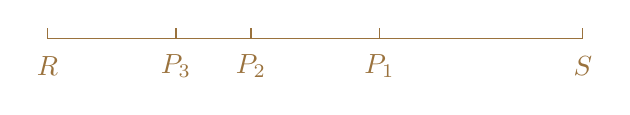
\begin{tikzpicture}[lichsutoanhoc,scale=0.68]
			\draw  (0.,0.)-- (10.,0.);
				\draw  (0.,0.) -- (0,0.2);
				\draw (0.0,-0.5) node {$R$};
				\draw  (10,0.) -- (10,0.2);
				\draw (10,-0.5) node {$S$};
				\draw  (6.2,0.) -- (6.2,0.2);
				\draw (6.2,-0.5) node {$P_1$};
				\draw  (3.8,0.) -- (3.8,0.2);
				\draw (3.8,-0.5) node {$P_2$};
				\draw  (2.4,0.) -- (2.4,0.2);
				\draw (2.4,-0.5) node {$P_3$};
		\end{tikzpicture}
		
		\vspace*{-5pt}
		\caption{\small\textit{\color{lichsutoanhoc}Hình $3$.}}
		\vspace*{-10pt}
	\end{figure}
	Tính chất này dẫn đến việc tiết lộ, có thể bởi Hippasus, về tính không thông ước giữa đường chéo của ngũ giác đều và cạnh của nó. Không có tài liệu nào khẳng định điều này, nhưng có vẻ như đây là một suy đoán có lý.
	\vskip 0.1cm
	Tỷ lệ giữa đường chéo của hình lập phương với một cạnh bằng $\sqrt{3}$, cũng dẫn tới tính không thông ước của đường chéo và cạnh của hình lập phương, hay tính chất vô tỷ của số $\sqrt{3}$.
	\begin{figure}[H]
		\vspace*{-10pt}
		\centering
		\captionsetup{labelformat= empty, justification=centering}
		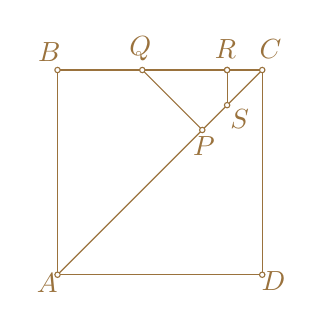
\begin{tikzpicture}[lichsutoanhoc,scale=0.65]
			\draw  (0.,0.)-- (4.,0.);
			\draw  (4.,0.)-- (4.,4.);
			\draw  (4.,4.)-- (0.,4.);
			\draw  (0.,4.)-- (0.,0.);
			\draw  (4.,4.)-- (0.,0.);
			\draw  (3.31370849898476,4.)-- (3.3137084989847594,3.3137084989847585);
			\draw  (1.6568542494923808,4.)-- (2.8284271247461903,2.82842712474619);
			
			\draw [fill=white] (0.,0.) circle (1.5pt);
			\draw (-0.2,-0.17) node {$A$};
			\draw [fill=white] (4.,0.) circle (1.5pt);
			\draw (4.22,-0.13) node {$D$};
			\draw [fill=white] (4.,4.) circle (1.5pt);
			\draw (4.16,4.41) node {$C$};
			\draw [fill=white] (0.,4.) circle (1.5pt);
			\draw (-0.16,4.35) node {$B$};
			\draw [fill=white] (1.6568542494923808,4.) circle (1.5pt);
			\draw (1.62,4.41) node {$Q$};
			\draw [fill=white] (3.31370849898476,4.) circle (1.5pt);
			\draw (3.28,4.41) node {$R$};
			\draw [fill=white] (3.31370849898476,4.) circle (1.5pt);
			\draw [fill=white] (3.3137084989847594,3.3137084989847585) circle (1.5pt);
			\draw (3.56,3.05) node {$S$};
			\draw [fill=white] (2.8284271247461903,2.82842712474619) circle (1.5pt);
			\draw (2.86,2.51) node {$P$};
		\end{tikzpicture}
	
		\vspace*{-5pt}
		\caption{\small\textit{\color{lichsutoanhoc}Hình $4$.}}
		\vspace*{-10pt}
	\end{figure}
	Tương tự như ngũ giác đều, nếu trong hình vuông $ABCD$ (Hình $4$) dựng trên đường chéo $AC$ đoạn $AP = AB$  và tại $P$ dựng đoạn thẳng $PQ$  vuông góc với đường chéo thì $\dfrac{CQ}{CP} = \dfrac{AC}{AB}$. Một lần nữa, nếu trên $CQ$  đặt $QR = QP$ và  dựng $RS$  vuông góc với $CR$,  thì  $\dfrac{CS}{CR} = \dfrac{CQ}{CP} = \dfrac{AC}{AB}$. Quá trình này có thể được lặp lại vô hạn. Đây một chứng minh cho thấy không có đơn vị độ dài nào, dù nhỏ, có thể được tìm thấy để đường chéo và cạnh hình vuông là thông ước với nhau.
	\vskip 0.1cm
	\PIbox{\textbf{\color{lichsutoanhoc}Bài tập.} Sử dụng chứng minh $\sqrt{2}$  là số vô tỷ (xem [$10$]), hãy chứng minh $\sqrt{3}$  là số vô tỷ, hay đường chéo của hình lập phương không thông ước với cạnh của nó. Tương tự, chứng minh $\sqrt{5}$ là số vô tỷ.}
	\vskip 0.1cm
	$\pmb{2.}$ \textbf{\color{lichsutoanhoc}Nghịch lý Zeno}
	\vskip 0.1cm
	Học thuyết Pythagoras cho rằng ``Các con số [hữu tỷ] tạo nên toàn bộ thiên đường" thực sự đã phải đối mặt với một vấn đề rất nghiêm trọng khi số vô tỷ được phát hiện, nhưng trường phái Pythagoras còn phải đối mặt với những lập luận do những học giả xứ Elea, một trường phái đối thủ đưa ra. 
	\vskip 0.1cm
	Các nhà triết học Ionia ở Tiểu Á đã tìm cách xác định yếu tố cơ bản của vật chất.
	\vskip 0.1cm
	Thales cho rằng nước là nguồn gốc của vật chất, nhưng những người khác ưu tiên coi không khí hoặc lửa là yếu tố cơ bản. Trường phái Pythagoras đã theo một hướng trừu tượng hơn: cho rằng các con số (hữu tỷ) là cơ bản. Thuyết này, được minh họa một cách tuyệt đẹp trong hình học của các con số tượng hình, đã bị công kích bởi những người theo Parmenides (đầu thế kỉ V TCN) xứ Elea. Nguyên lý cơ bản của trường phái Elea là sự thống nhất và vĩnh viễn, một quan điểm trái ngược với các ý tưởng của Pythagoras về tính đa dạng và thay đổi.  Trong các môn đệ của Parmenides, người được biết đến nhiều nhất là Zeno ở Elea (khoảng $495-430$ TCN), người đã đưa ra các lý lẽ để chứng minh sự mâu thuẫn trong các khái niệm của Pythagoras.
	\vskip 0.1cm
	Những người Pythagoras cho rằng không gian và thời gian có thể được coi là bao gồm các điểm và cá thể, nhưng không gian và thời gian cũng có thuộc tính, được gọi là ``tính liên tục". 
	Một mặt, tính liên tục có các đặc điểm của đơn vị hình học -- điểm -- và mặt khác, có các đặc điểm của các đơn vị số hoặc các số.
	Aristotle ($384-322$ TCN) đã mô tả quan điểm của Pythagoras là ``sự thống nhất có vị trí" hoặc ``sự thống nhất được xem xét trong không gian". 
	Để chống lại quan điểm này, Zeno đưa ra những nghịch lý, trong đó các nghịch lý về chuyển động dường như đã gây ra nhiều rắc rối nhất:
	\vskip 0.1cm
	$(1)$ Sự phân đôi (the Dichotomy), 
	\vskip 0.1cm
	$(2)$ Achilles và con rùa, 
	\vskip 0.1cm
	$(3)$ Mũi tên (the Arrow), và 
	\vskip 0.1cm
	$(4)$ Sân vận động (the Stade, hay Stadium).
	\vskip 0.1cm
	\textbf{\color{lichsutoanhoc}Sự phân đôi}
	\vskip 0.1cm
	Một người chạy được một quãng đường nhất định, trước tiên anh ta phải đi một nửa quãng đường này, nhưng trước khi anh ta có thể làm được điều này, anh ta phải đi một phần tư quãng đường đầu tiên, và trước đó, một phần tám quãng đường đầu tiên, và cứ như vậy, thông qua vô số đoạn.  Anh ta phải tạo vô số đoạn trong một thời gian hữu hạn, nhưng điều này là không thể. Do đó sự khởi động của chuyển động là không thể.
	\vskip 0.1cm
	\textbf{\color{lichsutoanhoc}Achilles và con rùa}
	\vskip 0.1cm
	Nghịch lý thứ hai tương tự như nghịch lý thứ nhất, ngoại trừ việc chia nhỏ vô hạn không gian là lũy tiến, chứ không phải là thoái lui. Giả sử Achilles chạy đua với một con rùa đã xuất phát từ trước. Khi Achilles đạt đến vị trí ban đầu của con rùa, thì con rùa đã đi được một đoạn ngắn và vào thời điểm Achilles vượt qua đoạn này, con rùa sẽ tiến lên hơi xa hơn, và quá trình này tiếp tục vô hạn, với kết quả là Achilles nhanh nhẹn không bao giờ có thể vượt qua con rùa chậm chạp.
	\vskip 0.1cm
	\textbf{\color{lichsutoanhoc}Mũi tên}
	\vskip 0.05cm
	Các nghịch lý \textit{Phân đôi} và \textit{Achilles} lập luận rằng chuyển động là không thể dưới giả thiết về sự chia nhỏ vô hạn không gian và thời gian. Mặt khác, \textit{Mũi tên} và \textit{Sân vận động} lập luận rằng chuyển động không thể xảy ra nếu giả định ngược lại rằng có một đại lượng nhỏ nhất của không gian và thời gian. Trong \textit{Mũi tên}, Zeno lập luận rằng một vật thể đang bay luôn chiếm một khoảng không gian bằng chính nó, nhưng chiếm một khoảng không gian bằng chính nó thì nó không chuyển động. Vì thế mũi tên đang bay luôn dừng lại, do đó chuyển động của nó chỉ là một ảo giác.
	\vskip 0.05cm
	\textbf{\color{lichsutoanhoc}Sân vận động}
	\vskip 0.05cm
	Gây tranh cãi nhiều nhất và khó xử nhất về những nghịch lý trong chuyển động là \textit{Sân vận động}, nó có thể được diễn giải như sau. 
	\vskip 0.1cm
	Giả sử rằng tại một thời điểm nhất định, các vật ${A_1}$, ${A_2}$, ${A_3}$, ${A_4}$, ${A_5}$, ${A_6}$, $A_7$, $A_8$; $B_1$, $B_2$, $B_3$, $B_4$, $B_5$, $B_6$, $B_7$, $B_8$  và $C_1$, $C_3$, $C_3,$ $C_4$, $C_5$, $C_6$, $C_7$, $C_8$ chiếm các vị trí tương đối sau \linebreak(Hình $5a$):
	\begin{figure}[H]
		\vspace*{-10pt}
		\centering
		\captionsetup{labelformat= empty, justification=centering}
		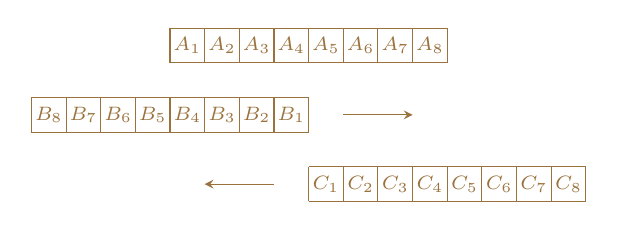
\begin{tikzpicture}[scale=0.44,lichsutoanhoc,node font=\scriptsize]
			\draw (0,0) grid (8,1);
			\draw (0,2) grid (-8,3);
			\draw (-4,4) grid (4,5);
			\draw[-stealth] (-1,0.5) -- (-3, 0.5);
			\draw[-stealth] (1,2.5) -- (3, 2.5);

			\foreach \x in {1,2,...,8}{
				\node at (\x-0.5, 0.5) {$C_\x$};
				\node at (\x - 4.5, 4.5) {$A_\x$};
				\node at (-\x + 0.5, 2.5) {$B_\x$};}
		\end{tikzpicture}
		\caption{\small\textit{\color{lichsutoanhoc}Hình $5a$: Sân vận động.}}
		\vspace*{-10pt}
	\end{figure}
	Các vật $B$ chuyển động sang phải và các vật $C$ chuyển động sang trái với cùng vận tốc để được Hình $5b$:
	\begin{figure}[H]
	\vspace*{-10pt}
	\centering
	\captionsetup{labelformat= empty, justification=centering}
	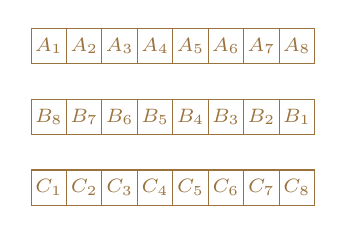
\begin{tikzpicture}[scale=0.45,lichsutoanhoc,node font=\scriptsize]
		\draw (0,0) grid (8,1);
		\draw (0,2) grid (8,3);
		\draw (0,4) grid (8,5);
		
		\foreach \x in {1,2,...,8}{
			\node at (\x-0.5, 0.5) {$C_\x$};
			\node at (\x-0.5, 4.5) {$A_\x$};
			\node at (8.5-\x, 2.5) {$B_\x$};}
	\end{tikzpicture}
	\caption{\small\textit{\color{lichsutoanhoc}Hình $5b$: Sân vận động.}}
	\vspace*{-10pt}
	\end{figure}
	Khi $C_1$  đi qua $8$ vật $B$  (và $B_1$ đi qua 8 vật  $C$) thì $B_1$  chỉ đi qua $4$ vật $A_5, A_6, A_7, A_8$  (tương tự,  $C_1$  đi qua $4$ vật  $A_1, A_2, A_3, A_4$). Nhưng $C_1$  mất cùng một thời gian khi đi qua $8$ vật  $B$ như là đi qua $4$ vật $A$.  Suy ra thời gian để  $C_1$  đi qua $8$ vật $A$  cũng bằng thời gian đi qua một nửa $A$,  hay thời gian đã cho bằng một nửa của nó. Mâu thuẫn.     
	\vskip 0.1cm
	Aristotle cho rằng Zeno đã không hiểu sự khác nhau giữa chuyển động tương đối với chuyển động tuyệt đối và tin rằng ông đã bác bỏ nghịch lý của Zeno vì ông đã phủ nhận giả định ban đầu: thời gian bao gồm các đơn vị không thể phân chia. Tuy nhiên, giải thích thấu đáo nghịch lý Zeno về sân vận động chỉ được đưa ra bởi Brochard, Noël và Russell vào thế kỉ XIX--XX.
	\vskip 0.1cm 
	Các lập luận của Zeno dường như đã có ảnh hưởng sâu sắc đến sự phát triển của toán học Hy Lạp, có thể so sánh với sự phát hiện ra số vô tỉ, mà chúng có thể có liên quan với nhau. Ban đầu, trong lý thuyết của Pythagoras, độ lớn được biểu thị bằng hạt hoặc đá cuội, nhưng đến thời Euclid thì có một sự thay đổi hoàn toàn về quan điểm.  Độ lớn nói chung không phải được liên kết với các con số hoặc viên sỏi, mà với các đoạn thẳng. Trong \textit{Cơ sở}, thậm chí các số nguyên cũng được biểu diễn bằng các đoạn. Vương quốc của con số có đặc tính rời rạc, nhưng thế giới của các đại lượng liên tục là một thứ ngoài số và phải được xử lý bằng phương pháp hình học (và điều này bao gồm hầu hết toán học thời kỳ tiền cổ đại và Pythagoras).  Dường như là hình học, hơn là con số, thống trị thế giới.
	\vskip 0.1cm
	$\pmb{3.}$ \textbf{\color{lichsutoanhoc}Học viện Plato}
	\vskip 0.1cm
	Thế kỷ thứ tư TCN đã mở đầu bằng cái chết của Socrates (khoảng $470-399$ TCN), một học giả đã áp dụng phương pháp biện chứng của Zeno và bác bỏ thuyết Pythagoras của Archytas (khoảng $420-347$ TCN). Socrates thừa nhận rằng khi còn trẻ, ông đã bị thu hút bởi những câu hỏi như tại sao tổng $2 + 2$ lại bằng tích $2 \times 2$  nhưng khi nhận ra rằng cả toán học và khoa học đều không thể thỏa mãn mong muốn của ông để  hiểu bản chất của sự vật, ông đã tự nghiên cứu để hiểu những điều bản chất.
	\end{multicols}
	\begin{figure}[H]
		\vspace*{5pt}
		\centering
		\captionsetup{labelformat= empty, justification=centering}
		\includegraphics[width= 1\linewidth]{H7}
		\caption{\small\textit{\color{lichsutoanhoc}Hình $6$: The School of Athens của Rafael tại Vaticant.}}
		\vspace*{-10pt}
	\end{figure}
	\begin{multicols}{2}
	Trong \textit{Phaedo} của Plato, cuộc đối thoại trong đó những giờ cuối cùng của Socrates được mô tả rất đẹp, chúng ta thấy những nghi ngờ siêu hình sâu sắc như thế nào loại trừ mối quan tâm của Socrate về toán học hoặc khoa học tự nhiên:
	\vskip 0.1cm
	\textit{Tôi không thể tự thỏa mãn bản thân rằng, khi một cái được thêm vào một cái, mà phép cộng được thực hiện trở thành hai. 
	\vskip 0.1cm
	Tôi không thể hiểu làm thế nào khi tách khỏi nhau, mỗi trong số chúng là một chứ không phải hai, và bây giờ, khi chúng được kết hợp lại với nhau, chỉ là sự đặt cạnh nhau, là nguyên nhân khiến chúng trở thành hai.}
	\vskip 0.1cm
	Do đó, ảnh hưởng của Socrates trong sự phát triển của toán học là không đáng kể, nếu không nói là tiêu cực. Điều đáng ngạc nhiên là chính học trò và người ngưỡng mộ ông là Plato đã trở thành cảm hứng toán học của thế kỷ thứ tư TCN. 
	\vskip 0.1cm
	Mặc dù bản thân Plato không có đóng góp kết quả toán học nổi bật cụ thể nào, nhưng ông đã là trung tâm của hoạt động toán học thời gian đó, hướng dẫn và truyền cảm hứng cho sự phát triển của toán học. Tại cửa trường học của ông, Học viện (The Academy) ở Athens, được khắc khẩu hiệu ``Ai không biết hình học không vào đây".
	\vskip 0.1cm
	\PIbox{ΑΓΕΩΜΕΤΡΗΤΟΣ ΜΗΔΕΙΣ ΕΙΣΙΤΩ.}
	\vskip 0.1cm
	Sự nhiệt tình của Plato đối với toán học khiến ông được biết đến không phải với tư cách là một nhà toán học, mà là ``người tạo ra các nhà toán học".
	\vskip 0.1cm
	Sáu nhà toán học (ngoài Plato và Aristotle) sống giữa năm mất của Socrates ($399$ TCN) và năm mất của Aristotle ($322$ TCN) -- gồm Theodorus xứ Cyrene (thế kỉ V TCN), Theaetetus (khoảng $414-369$ TCN), Eudoxus xứ Cnidus (khoảng $410-347$ TCN), hai anh em Menaechmus ($380-320$ TCN) và Dinostratus ($390-320$  TCN), và Autolycus xứ Pitane ($360-320$ TCN) -- là những nhà toán học đã có liên kết ít nhiều chặt chẽ với Học viện Plato.
	\vskip 0.1cm
	Rõ ràng là việc Plato rất coi trọng toán học không đến từ Socrates. Trên thực tế, các bài giảng trong thời kỳ đầu và tác phẩm Đối thoại (Dialogues) của Plato hiếm khi đề cập đến toán học. Archytas, một người bạn của Plato, là người đã khiến Plato quan tâm đến toán học, khi Ông đến thăm bạn ở Sicily vào năm $388$ TCN. Có lẽ chính khi đó, Plato mới biết đến năm hình đa diện đều, được liên kết với bốn nguyên tố (nước, lửa, không khí và đất) của Empedocles ($490-430$ TCN) trong một sơ đồ vũ trụ đã mê hoặc các nhà nghiên cứu trong nhiều thế kỉ (Hình $7$). 
	\vskip 0.1cm
	Có thể, sự coi trọng của Pythagoras đối với khối $12$ mặt đều đã khiến Plato xem xét nó, khối đa diện đều thứ năm và cuối cùng, như một biểu tượng của vũ trụ. 
	Plato đặt ý tưởng của ông về đa diện đều thành một cuộc đối thoại có tiêu đề \textit{Timaeus}, được đặt tên cho một người đóng vai trò là người đối thoại chính thuộc trường phái Pythagoras. Không biết Timaeus xứ Locri có thực sự tồn tại không, hay Plato đã phát minh ra Timaeus như một nhân vật để thể hiện quan điểm của Pythagoras, khi ấy vẫn còn mạnh mẽ ở khu vực mà ngày nay là nước Ý. 
	\begin{figure}[H]
		\vspace*{-5pt}
		\centering
		\captionsetup{labelformat= empty, justification=centering}
		\begin{tikzpicture}[scale=0.8, lichsutoanhoc, node font=\small]
			\draw  (0.,0.)-- (3.,3.);
			\draw  (3.,3.)-- (0.,6.);
			\draw  (0.,6.)-- (-3.,3.);
			\draw  (-3.,3.)-- (0.,0.);
			\draw [dashed] (0.,0.)-- (0.,6.);
			\draw [dashed] (-3.,3.)-- (3.,3.);
			\draw[color=black] (1.9,1.45) node {\color{lichsutoanhoc}Ẩm};
			\draw[color=black] (1.8,4.91) node {\color{lichsutoanhoc}Nóng};
			\draw[color=black] (-1.75,4.91) node {\color{lichsutoanhoc}Khô};
			\draw[color=black] (-1.95,1.33) node {\color{lichsutoanhoc}Lạnh};
			\draw(0,6) node[above] {Lửa -- Tứ diện đều};
			\draw(0,0) node[below] {Nước -- Khối $20$ mặt đều};
			\draw(3.4,3) node[rotate=-90] {Đất -- Lập phương};
			\draw(-3.2,3) node[rotate=90] {Không Khí -- Bát diện đều};
		\end{tikzpicture}
		\caption{\small\textit{\color{lichsutoanhoc}Hình $7$: Sơ đồ vũ trụ ứng với khối đa diện.}}
		\vspace*{-10pt}
	\end{figure}
	Các khối đa diện đều thường được gọi là ``vật thể vũ trụ" hoặc ``khối đa diện Plato" bởi vì cách mà Plato trong \textit{Timaeus} đã áp dụng chúng vào giải thích các hiện tượng khoa học.
	\vskip 0.1cm
	Mặc dù đối thoại này, có lẽ được viết khi Plato đã gần bảy mươi tuổi, cung cấp bằng chứng xác thực sớm nhất cho sự liên kết của bốn nguyên tố với khối đa diện đều, phần lớn sự tưởng tượng này có thể là do trường phái Pythagoras.
	\vskip 0.1cm
	Proclus (khoảng $410-485$) quy việc xây dựng hình học vũ trụ cho Pythagoras, nhưng có thể bạn của Plato là Theaetetus (khoảng $414-369$ TCN) đã viết về liên kết giữa vũ trụ và khối đa diện đều. 
	\vskip 0.1cm
	Quyển XIII của \textit{Cơ sở} của Euclid nói rằng chỉ có ba trong số năm khối đa diện là do Pythagoras, và nhờ Theaetetus mà khối bát diện và hai mươi mặt đều đã được biết đến.
	\vskip 0.1cm
	Có vẻ như Theaetetus đã thực hiện một trong những nghiên cứu quy mô nhất về năm khối đa diện, và định lý nói rằng có và chỉ có năm khối đa diện đều là thuộc về Theaetetus. Có lẽ ông cũng là tác giả của các tính toán về tỷ lệ các cạnh của khối đa diện đều và bán kính mặt cầu ngoại tiếp. 
	\vskip 0.1cm
	Theaetetus là một thanh niên Athens chết vì bệnh kiết lỵ kết hợp với vết thương trong trận chiến, và cuộc đối thoại của Plato mang tên ông là một sự tưởng nhớ của Plato đối với người bạn của mình.
	\vskip 0.1cm
	Trong cuộc đối thoại, có bối cảnh trước đó khoảng ba mươi năm, Theaetetus thảo luận với Socrates và Theodorus về bản chất của các đại lượng vô ước với nhau (hay các đại lượng không thông ước với nhau). Người ta đã giả định rằng cuộc thảo luận này phần nào có dạng mà chúng ta tìm thấy trong phần mở đầu của Quyển X của \textit{Cơ sở}.
	\vskip 0.1cm
	Ở đây, sự phân biệt không chỉ được thực hiện giữa các đại lượng thông ước và vô ước, mà còn giữa các đại lượng khi độ dài là vô ước với nhau, nhưng có diện tích thông ước với nhau. Như $\sqrt{3}$  và $\sqrt{5}$  không thông ước về độ dài, nhưng thông ước về diện tích, vì các hình vuông của chúng có tỷ lệ là $3/5$.
	\vskip 0.1cm
	Mặt khác, các đại lượng  $\sqrt{1 + \sqrt{3}}$  và $\sqrt{1 + \sqrt{5}}$ là không thông ước cả về độ dài và diện tích.
	\vskip 0.1cm
	Cuộc đối thoại mà Plato sáng tác để tưởng nhớ người bạn Theaeteus của mình chứa thông tin về một nhà toán học khác, Theodorus xứ Cyrene, thầy của Plato và Theaetetus, người mà Plato ngưỡng mộ và là người đã đóng góp vào sự phát triển của lý thuyết về các đại lượng vô ước. 
	\vskip 0.1cm
	Không biết bằng cách nào mà Theodorus đã làm điều này và tại sao ông lại dừng lại ở $\sqrt{17}$ 
	\vskip 0.1cm
	Theodorus là người đầu tiên chứng minh tính vô tỷ của căn bậc hai của các số nguyên không chính phương từ $3$ đến $17$.	 
	\vskip 0.1cm
	Chứng minh, trong mọi trường hợp, được đưa ra bởi Aristotle khi ông xây dựng trục xoắn ốc dọc theo đoạn $\sqrt{2}$. Các tác phẩm lịch sử cổ đại chỉ ra rằng Theodorus đã khám phá ra điều này và sau này nó được đưa vào \textit{Cơ sở}, nhưng các tác phẩm của Theodorus đã bị mất. 
	\begin{figure}[H]
		\vspace*{-5pt}
		\centering
		\captionsetup{labelformat= empty, justification=centering}
		\includegraphics[width= 0.85\linewidth]{H8}
		\caption{\small\textit{\color{lichsutoanhoc}Hình $8$: Xoắn ốc Theodorus.}}
		\vspace*{-10pt}
	\end{figure}
	Plato có vai trò quan trọng trong lịch sử toán học phần lớn vì ông là người truyền cảm hứng và là người sáng lập Học viện đào tạo ra nhiều nhà toán học, cũng như do sự nhạy bén của ông về sự phân biệt ở Hy Lạp cổ đại giữa số học (theo nghĩa của lý thuyết về các con số) và kỹ thuật tính toán. 
	\vskip 0.1cm
	Plato cho rằng toán học là cần thiết cho doanh nhân và quân sự, ``phải học nghệ thuật của những con số, nếu không anh ta sẽ không biết cách dàn quân".
	\vskip 0.1cm
	Mặt khác, nhà triết học phải là một nhà số học ``bởi vì anh ta phải nhảy ra khỏi biển của những thay đổi và nắm giữ bản thể đích thực." Hơn nữa, Plato nói trong tác phẩm \textit{Cộng hòa (The Republic)}: ``Số học có tác dụng rất lớn và nâng cao, buộc tâm trí nghĩ về số trừu tượng."
	\vskip 0.1cm 
	Trong số học, Plato đã nhìn thấy một hố ngăn cách lý thuyết và các khía cạnh tính toán, cũng như trong hình học, ông cũng tán thành toán học thuần túy chống lại quan điểm duy vật.  
	\vskip 0.1cm
	Bất kỳ một trong số vô số đường kính của đường tròn là trục đối xứng của hình. Bất cứ điểm nào trên một đường thẳng kéo dài vô hạn có thể được coi là tâm của đối xứng, giống như bất kỳ đường thẳng nào vuông góc với đường thẳng đã cho là trục đối xứng của đường thẳng đã cho. Triết học Plato, với sự áp dụng các ý tưởng của nó, tự nhiên sẽ tìm thấy vai trò của đường thẳng và đường tròn giữa các hình hình học. Tương tự, Plato tôn vinh tam giác.
	\vskip 0.1cm 
	Sự liên kết của bốn khối đa diện đầu tiên với bốn yếu tố phổ quát truyền thống của vũ trụ đã cung cấp cho Plato trong \textit{Timaeus}  một lý thuyết thống nhất tuyệt đẹp về vật chất, theo đó mọi thứ đều được xây dựng bằng các tam giác vuông lý tưởng. Toàn bộ sinh lý học, cũng như khoa học về chất trơ, dựa trên các hình tam giác.
	\vskip 0.1cm
	Pythagoras nổi tiếng là người đã thiết lập toán học như một chủ đề tự do, nhưng Plato đã có ảnh hưởng trong việc làm cho toán học trở thành một phần thiết yếu của chương trình đào tạo.
	\vskip 0.1cm
	Có lẽ bị ảnh hưởng bởi Archytas, Plato đã thêm vào các chủ đề ban đầu trong bộ bốn (quadrivium: Số học, Hình học, Âm nhạc, Thiên văn) một môn học mới: Hình học không gian, vì ông tin rằng hình học không gian đã không được nhấn mạnh đầy đủ. Plato cũng thảo luận về nền tảng của toán học, làm rõ một số định nghĩa và xây dựng lại các giả thiết. Ông nhấn mạnh rằng lý luận được sử dụng trong hình học không đề cập đến những con số hữu hình mô tả chúng, mà là những ý tưởng tuyệt đối mà chúng đại diện. 
	\vskip 0.1cm
	Những người theo thuyết Pythagoras đã định nghĩa điểm là ``sự thống nhất có vị trí," nhưng Plato lại nghĩ về nó như là sự khởi đầu của một đường thẳng.
	\vskip 0.1cm 
	Định nghĩa của một đường là ``chiều dài không có chiều rộng" dường như bắt nguồn từ trường phái Plato.
	\vskip 0.1cm
	Trong số học, Plato không chỉ nhấn mạnh sự phân biệt giữa số lẻ và số chẵn, mà còn là các loại ``chẵn nhân chẵn", ``chẵn nhân lẻ" và ``lẻ nhân lẻ". Mặc dù ta biết rằng Plato đã thêm vào các tiên đề của toán học, chúng ta không có một cơ sở nào để khẳng định điều này.
	\vskip 0.1cm
	Rất ít đóng góp toán học cụ thể được quy cho Plato. Một công thức cho bộ ba Pythagoras -- ${(2n)^2} + {({n^2} - 1)^2} = {({n^2} + 1)^2}$, trong đó  $n$ là số tự nhiên bất kỳ -- mang tên Plato, nhưng đây chỉ là một phiên bản sửa đổi của kết quả được người Babylon và người Pythagoras đã biết. 
	\vskip 0.1cm
	Có lẽ thực sự có ý nghĩa quan trọng hơn cả trong những thứ được gán cho Plato là cái gọi là phương pháp phân tích (analytic method).
	\vskip 0.1cm
	Trong chứng minh toán học, ta bắt đầu với những gì đã cho, và từ các tiên đề và các định đề. Tiến hành từng bước một, sau đó đến khẳng định cần được chứng minh.
	\vskip 0.1cm
	Plato dường như đã chỉ ra rằng  về mặt sư phạm, khi không tìm được một chuỗi lý luận hiển nhiên từ giả thiết đến kết luận, thường là thuận tiện hơn nếu ta bắt đầu bằng mệnh đề cần được chứng minh và từ đó suy ra một kết luận được biết là đúng. Nếu, sau đó, có thể đảo ngược các bước trong chuỗi lý luận này, kết quả sẽ là mệnh đề đã được chứng minh.
	\vskip 0.1cm
	Plato không hẳn là người đầu tiên nêu lên quan điểm phân tích.  Nhưng những gì Plato có thể đã làm là chính thức hóa quá trình này, hoặc có thể ông đã đặt tên cho nó.
	\vskip 0.1cm
	Vai trò của Plato trong lịch sử toán học vẫn còn bị tranh cãi gay gắt. Một số người coi ông là một nhà tư tưởng đặc biệt sâu sắc và nhạy bén. Những người khác hình dung ông như một người đã thu hút các nhà toán học theo con đường lí luận trừu tượng, đi xa những vấn đề thực tiễn. 
	\vskip 0.1cm
	Trong mọi trường hợp, ít ai có thể phủ nhận rằng Plato đã có tác động to lớn đối với sự phát triển của toán học. Học viện Plato ở Athens trở thành trung tâm toán học của thế giới, và từ ngôi trường này, xuất hiện các giáo viên và nghiên cứu viên hàng đầu đến vào giữa thế kỷ thứ tư TCN. Trong số này, nổi tiếng nhất là Eudoxus xứ Cnidus (khoảng $408-335$ TCN),  một học trò của Plato và người đã trở thành nhà toán học và nhà thiên văn học nổi tiếng nhất trong thời đại của mình.
	\vskip 0.1cm
	\textbf{\color{lichsutoanhoc}Tài liệu chính dùng để soạn}
	\vskip 0.1cm
	[$1$] David M. Burton, \textit{The History of Mathematics, An Introduction}, Seventh Edition, McGraw--Hill, $2011$. Chapter $3$: The Beginnings of Greek Mathematics, pp. $116-139$.
	\vskip 0.1cm
	[$2$] Euclid’s \textit{Elements of Geometry}, edited and provided with a modern English translation by Richard Fitzpatrick, Independently published, $2008$, $544$ p.
	\vskip 0.1cm
	[$3$] David Fowler, \textit{The Mathematics of Plato’s Academy}, Second Edition, Clarendon Press, Oxford, $1999$, $441$ p.
	\vskip 0.1cm   
	[$4$] Thomas Heath, \textit{A History of Greek Mathematics}, Oxford at the Clarendon Press, $1921$, Volume $1$: From Thales to Euclid, pp. $170-315$.
	\vskip 0.1cm   
	[$5$] Victor J. Katz, \textit{A History of Mathematics, An Introduction}, Third Edition, Addison--Wesley, $2009$. Chapter $2$: \textit{The Beginnings of Mathematics in Greek}, pp. $40-49$.
	\vskip 0.1cm
	[$6$] Uta C. Merzbach and Carl B. Boyer, \textit{A
	History of Mathematics}, Third Edition, John Wiley \& Sons, $2011$, pp. $65-80$.
	\vskip 0.1cm
	[$7$] George Johston Allman, \textit{Greek Geometry, From Thales to Euclid}, Dublin Universty Press, $1885$, $432$ p.
	\vskip 0.1cm  
	[$8$] R. Lloyd, \textit{Early Greek Science: Thales to Aristotle}, $1970$, Chatto \& Windus, London, $156$ p.
	\vskip 0.1cm 
	[$9$] Arpad Szabo, \textit{The beginnings of Greek Mathematics}, Springer, $1978$, $363$ p.
	\vskip 0.1cm
	\textbf{\color{lichsutoanhoc}Tài liệu trích dẫn}
	\vskip 0.1cm
	[$10$] Tạ Duy Phượng, \textit{Pythagoras và trường phái toán học Pythagoras}, Tạp chí Pi, Tập $6$ ($2022$), số $5$, trang $45-53$.
\end{multicols}
	 \newpage
%
%	 \setcounter{figure}{0}
%	 \thispagestyle{timhieukhoahocnone}
\pagestyle{timhieukhoahoc}
\everymath{\color{timhieukhoahoc}}
\blfootnote{$^1$\text{\color{timhieukhoahoc}Viện Sinh thái và Môi trường Đông Dương.}}
\graphicspath{{../timhieukhoahoc/pic/}}
\begingroup
\AddToShipoutPicture*{\put(0,616){\includegraphics[width=19.3cm]{../bannertimhieu}}}
\AddToShipoutPicture*{\put(108,522){\includegraphics[scale=1]{../tieude.pdf}}}
\centering
\endgroup
\vspace*{185pt}

\begin{multicols}{2}
	Nhắc đến Mendel, người ta thường nghĩ đến các bài tập về di truyền liên quan đến tổ hợp và xác suất trong môn sinh học. Tuy nhiên, bối cảnh lịch sử cũng như sự liên hệ của các định luật Mendel với các vấn đề khác trong sinh học lại thường ít được các tài liệu chú trọng giới thiệu. Nhân dịp kỷ niệm $200$ năm ngày sinh Mendel ($20/07/1822$ -- $20/07/2022$), chúng ta hãy cùng tìm hiểu về thí nghiệm lai giống đậu kinh điển của ông, vai trò của thống kê và tổ hợp trong thí nghiệm này cùng một số vấn đề xung quanh sự ra đời của di truyền học.
	\begin{figure}[H]
		\centering
		\vspace*{-5pt}
		\captionsetup{labelformat= empty, justification=centering}
		\includegraphics[width=1\linewidth]{image011}
		\vspace*{-15pt}
	\end{figure}
	$\pmb{1.}$ \textbf{\color{timhieukhoahoc}Giai đoạn ban đầu}
	\vskip 0.1cm
	Johann Mendel sinh năm $1822$ tại Heizendorf, vùng Silesia, thuộc đế quốc Áo (ngày nay thuộc cộng hòa Czech). Ông được gia đình cho đi học đến năm $21$ tuổi nhưng do hoàn cảnh tài chính, ông lựa chọn trở thành tu sĩ ở một tu viện ở Brno và đổi tên thành Gregor.
	\vskip 0.1cm
	Sau một thời gian, ông được tu viện phân công dạy khoa học tự nhiên tại trường học của nhà thờ ở Znojmo, một địa phương gần đó. Công việc này cũng phù hợp với sự yêu thích khoa học sẵn có của Mendel. 
	\vskip 0.1cm
	Đến năm $1849$, chính phủ Áo yêu cầu tất cả các giáo viên cần phải trải qua kỳ thi để cấp chứng chỉ hành nghề. Tuy Mendel không vượt qua được kỳ thi khảo sát do Đại học Vienna tổ chức, ông vẫn đủ tiêu chuẩn để được theo học tại đây dưới dạng sinh viên dự thính.Trong giai đoạn từ $1851$ đến $1853$, Mendel theo học nhiều môn khác nhau: vật lý, hóa học, toán học, động vật học, thực vật học và cổ sinh học. Trong quá trình đó, ông được tiếp cận với các bài giảng của Franz Unger, một nhà thực vật học nổi tiếng lúc đó. Dựa trên các nghiên cứu về hóa thạch cổ đại cùng những kiến thức mới về tế bào và sự phát triển phôi ở thực vật, Unger đưa ra một mô hình về sự tiến hóa của sinh vật: theo đó, một loài không tự nhiên sinh ra mà là hậu duệ của một loài trước đó và sự tiến hóa không tiến hành theo dạng tuyến tính mà có dạng hình cây. Unger chịu nhiều chỉ trích từ các nhân vật bảo thủ do quan điểm này ngược với các giải thích dựa trên tôn giáo. Dù bản thân là một thành viên của nhà thờ, Mendel vẫn tham gia học ở lớp của Unger.
	\vskip 0.1cm
	Tháng $8$ năm $1853$, Mendel trở lại tu viện ở Brno. Môi trường ở đây vẫn luôn chịu sự kiểm duyệt của giáo hội với các cuộc thanh tra, trong đó Mendel bị nhận định là dạng cá biệt, chuyên nghiên cứu ``các khoa học vớ vẩn". Năm $1856$, Mendel trở lại Vienna để tham dự kỳ thi sát hạch giáo viên lần thứ hai. Tuy nhiên, ông bị ốm nặng sau câu hỏi đầu tiên và phải trở về nằm giường ở Brno một thời gian. Dù mong muốn trở thành giáo viên dạy khoa học bị tan vỡ, Mendel vẫn không từ bỏ và tiến hành một thí nghiệm mà ông đã ấp ủ từ trong vài năm trước.
	\begin{figure}[H]
		\centering
		\vspace*{-5pt}
		\captionsetup{labelformat= empty, justification=centering}
		\includegraphics[width=1\linewidth]{image002}
		\caption{\small\textit{\color{timhieukhoahoc}Hình $1$. Loài đậu Pisum sativum.}}
		\vspace*{-10pt}
	\end{figure}
	Mendel tiến hành thí nghiệm để tìm hiểu các vấn đề về sự lai giống của sinh vật, một chủ đề ông được tiếp xúc trong quá trình học ở Đại học Vienna. Đối tượng của ông là loài đậu \textit{Pisum sativum}, với các dòng thuần đã được Mendel chọn lọc trong vòng hai năm trước~đó.
	\vskip 0.1cm
	$\pmb{2.}$ \textbf{\color{timhieukhoahoc}Thí nghiệm trên cây đậu}
	\vskip 0.1cm
	Quá trình thí nghiệm của Mendel được tiến hành trong suốt $8$ năm từ $1856$ đến $1863$. Trong các giống đậu đã nhân được, ông chọn ra $22$ giống để tiến hành thí nghiệm. Chúng đã được kiểm chứng là dòng thuần. Mendel sử dụng $7$ đặc điểm để phân biệt chúng, mỗi đặc điểm có hai dạng khác nhau. Các đặc điểm về hạt (màu sắc và bề mặt) có thể được quan sát trực tiếp trên các hạt đậu. Các đặc điểm còn lại yêu cầu việc gieo hạt và quan sát cây trưởng thành.
	\vskip 0.1cm
	$\pmb{2.1}$ \textbf{\color{timhieukhoahoc}Tỷ lệ trong lai giống}
	\vskip 0.1cm
	Đầu tiên, Mendel tiến hành lai các dòng thuần (F$0$) với nhau để cho ra thế hệ lai F$1$. Kết quả cho thấy với mỗi một đặc điểm, sẽ có một dạng trội mà tất cả các F$1$ đều biểu hiện theo dạng này, dạng còn lại trở thành dạng lặn. Tiếp theo, Mendel cho các F$1$ tự thụ phấn để sinh ra các F$2$. Kết quả thống kê cho thấy tỷ lệ trội~:~lặn ở F2 gần với tỷ lệ $3$~:~$1$ cho cả $7$ đặc điểm. Đặc biệt, khi cho hạt của cùng một cây F$1$ hoặc trong cùng một quả mọc lên, dạng trội và dạng lặn đều có thể xuất hiện.
	\vskip 0.1cm
	Mendel lại tiếp tục cho các cây F$2$ tự thụ phấn để cho ra thế hệ F$3$. Ông nhận thấy rằng các F$2$ mang đặc điểm lặn cho ra thế hệ F$3$ giống như vậy. Trong các cây F$2$ mang đặc điểm trội, $2/3$ trong số chúng có F$3$ theo tỷ lệ trội~:~lặn là $3$~:~$1$, giống với khi lai hai dòng thuần; còn $1/3$ còn lại cho F$3$ toàn bộ trội (các tỷ lệ này đã được làm tròn từ dữ liệu thống kê). Từ kết quả này, Mendel nhận thấy khi lai các cây lai F$1$, một nửa các hạt thu được (F$2$) sẽ là dạng lai giống như F$1$ còn một nửa còn lại trở thành dòng thuần trội hoặc dòng thuần lặn (giống F$0$) với số lượng như nhau.
	\vskip 0.1cm
	Ông tiến hành lặp lại các thí nghiệm trên các đặc điểm của hạt đậu cho $6$ thế hệ và trên các đặc điểm của cây đậu cho $4$ thế hệ liên tiếp. Kết quả cho cả $7$ đặc điểm khẳng định rằng thế hệ sau của các cây lai từ hai dòng thuần được phân chia theo tỷ lệ $2$~:~$1$~:~$1$ cho dạng lai và hai dạng thuần.
	\vskip 0.1cm
	Mendel ký hiệu $A$ là dạng trội, $a$ là dạng lặn và $Aa$ là dạng lai kết hợp của hai dạng thuần (Tất nhiên là lúc đó Mendel không thể biết được việc vật liệu di truyền có hai bản sao theo cặp. Theo cách ký hiệu ngày nay, các ký hiệu trên phải là $AA$, $aa$ và $Aa$). Ông biểu diễn thế hệ F$2$ theo biểu thức: $A + 2Aa + a$.
	\begin{figure}[H]
		\centering
		\vspace*{-5pt}
		\captionsetup{labelformat= empty, justification=centering}
		\includegraphics[width=1\linewidth]{image003}
		\caption{\small\textit{\color{timhieukhoahoc}Hình $2$. Các đặc điểm Mendel nghiên cứu trong thí nghiệm lai cùng tỷ lệ trội~:~lặn quan sát được.}}
		\vspace*{-10pt}
	\end{figure}
	$\pmb{2.2}$ \textbf{\color{timhieukhoahoc}Lai nhiều đặc điểm}
	\vskip 0.1cm
	Mendel lại tiếp tục tiến hành thí nghiệm về sự tương tác giữa nhiều hơn một đặc điểm khác nhau khi lai. Trong thí nghiệm cho hai đặc điểm, Mendel lai dòng thuần hạt tròn $(A)$ -- hạt vàng $(B)$ với dòng thuần hạt nhăn $(a)$ -- hạt xanh $(b)$. Ở đây, các chữ cái in biểu diễn dạng trội còn các chữ cái thường biểu diễn dạng lặn của một đặc điểm. Kết quả cho F$1$ toàn bộ có hạt tròn và vàng. Khi cho $15$ cây F$1$ tự thụ phấn, Mendel thu được $556$ hạt F$2$. Các F$2$ này được trồng thành cây và đặc điểm của các hạt của chúng (tức F$3$) được thống kê để phân loại F$2$.
	\begin{table}[H]
		\vspace*{-5pt}
		\centering
		\captionsetup{labelformat= empty, justification=centering}
		\resizebox{\columnwidth}{!}{\begin{tabular}{|l|p{1.6cm}|p{2cm}|p{1.6cm}|}
			\hline
			&$A$&	$Aa$&	$A$\\
			\hline
			$B$&	$AB$ (tròn vàng)~:~$38$&	$AaB$ (tròn vàng + nhăn vàng)~:~$60$&	$aB$ (nhăn vàng)~:~$28$\\
			\hline
			$Bb$&	$ABb$ (tròn vàng + tròn xanh)~:~$65$&	$AaBb$ (tròn vàng + tròn xanh + nhăn vàng + nhăn xanh)~:~$138$&	$aBb$ (nhăn vàng và nhăn xanh)~:~$68$\\
			\hline
			$b$&	$Ab$ (tròn xanh)~:~$35$& $Aab$ (tròn xanh + nhăn xanh)~:~$67$&	$ab$ (nhăn xanh)~:~$30$\\
			\hline
		\end{tabular}}
		\caption{\small\textit{\color{timhieukhoahoc}Bảng $1$. Kết quả phân loại $556$ cây F$2$ dựa trên hạt của chúng.}}
		\vspace*{-10pt}
	\end{table}
	Mendel phân loại các dạng thu được thành ba nhóm: nhóm có cả hai đặc điểm đều là thuần ($AB$, $Ab$, $aB$ và $ab$), nhóm có một đặc điểm thuần và một đặc điểm lai ($ABb$, $aBb$, $AaB$, $Aab$) và nhóm có cả hai đặc điểm là lai ($AaBb$). Ông nhận định rằng số liệu của các dạng này: $32$, $65$, $138$ gần với bộ số $33$, $66$, $132$ ứng với tỷ lệ $1 : 2 : 4$. Có thể thấy trực giác phân tích số liệu của Mendel rất tốt. Ông kết luận rằng hiện tượng quan sát được là do sự kết hợp của hai biểu thức $A + 2Aa + a$ và $B + 2Bb +b$. Thật vậy, tiến hành phép nhân hai biểu thức này, ta được:
	\begin{align*}
		&AB + 2AaB + aB + 2ABb +4AaBb\\
		&+ 2aBb + Ab + 2Aab + ab
	\end{align*}
	Tương tự, khi tiến hành thí nghiệm lai cho ba đặc điểm, kết quả phân bố cũng phù hợp với tích của ba biểu thức $A + 2Aa + a$, $B + 2Bb +b$ và $C + 2Cc + c$.
	\vskip 0.1cm
	Một điểm tương đối thú vị ở đây là Mendel không sử dụng công thức nhân xác suất như ngày nay ta vẫn dùng khi giải các bài toán tổ hợp trong di truyền mà biểu diễn số lượng các nhóm trong mỗi đặc điểm theo biểu thức đại số với các hệ số có tỷ lệ ứng với số lượng từng nhóm rồi tiến hành nhân các biểu thức đại số để cho ra tỷ lệ giữa các nhóm tổ hợp.
	\vskip 0.1cm
	Các kết quả của hai thí nghiệm này (cũng như nhiều thí nghiệm tương tự cho các bộ đặc điểm khác) cho phép Mendel kết luận rằng việc di truyền các đặc điểm mà ông nghiên cứu là độc lập.
	\vskip 0.1cm
	$\pmb{2.3}$ \textbf{\color{timhieukhoahoc}Thí nghiệm về tế bào sinh sản}
	\vskip 0.1cm
	Trong các thí nghiệm trước, khi tiến hành lai các F$0$, Mendel đem phấn từ các cây dòng thuần lặn đến thụ phấn cho hoa của các cây dòng thuần trội. Câu hỏi đặt ra là nếu vai trò hoa/phấn hoa được đảo lại thì kết quả có vẫn luôn vậy không? Ông giả định rằng số loại tế bào noãn/phấn hoa được tạo ra bằng với số lượng các dạng tổ hợp của các dòng thuần (ví dụ $AB$, $Ab$, $aB$, $ab$ cho trường hợp hai đặc điểm). Đồng thời khi kết hợp giả định này với việc tỷ lệ của mỗi tổ hợp so với tổng số là giống nhau, Mendel hy vọng nó có thể giải thích các kết quả về phân bố tổ hợp của các đặc điểm ở những thí nghiệm trước đó.
	\vskip 0.1cm
	Đầu tiên Mendel thụ phấn cho hoa của F$0$ trội $AB$ bằng phấn từ cây F$0$ lặn $ab$ để thu được dạng lai $AaBb$. Tiếp đó, ông tiến hành $4$ quá trình thụ phấn:
	\vskip 0.1cm
	$\bullet$ cho hoa của dạng lai từ phấn hoa của $AB$
	\vskip 0.1cm
	$\bullet$ cho hoa của dạng lai từ phấn hoa của $ab$
	\vskip 0.1cm
	$\bullet$ cho hoa của $AB$ từ phấn hoa của dạng lai
	\vskip 0.1cm
	$\bullet$ cho hoa của ab từ phấn hoa của dạng lai
	\vskip 0.1cm
	Với mỗi thí nghiệm, tất cả hoa của một cây đều được thụ phấn. Mendel nhận định rằng nếu giả định của mình là đúng thì các cây lai sẽ có các tế bào noãn và tế bào phấn hoa của các dạng $AB$, $Ab$, $aB$, và $ab$. Khi chúng kết hợp với các tế bào noãn và tế bào phấn hoa từ các cây bố mẹ $AB$ và $ab$ thì sẽ có các mẫu lần lượt như sau trong từng trường hợp:
	\vskip 0.1cm
	$\bullet$ $AB$, $ABb$, $AaB$, $AaBb$
	\vskip 0.1cm
	$\bullet$ $AaBb$, $Aab$, $aBb$, $ab$
	\vskip 0.1cm
	$\bullet$ $AB$, $ABb$, $AaB$, $AaBb$
	\vskip 0.1cm
	$\bullet$ $AaBb$, $Aab$, $aBb$, $ab$
	\vskip 0.1cm
	và trong mỗi trường hợp, các dạng đều xuất hiện với tần số như nhau.
	\vskip 0.1cm
	Mendel nhận thấy kết quả thí nghiệm không phụ thuộc vào việc phấn hoa được lấy từ dòng thuần nào khi tiến hành lai F$0$. Tất nhiên, ông cũng chỉ ra rằng số liệu thống kê từ thí nghiệm không thể hoàn toàn khớp một cách chính xác như công thức toán học.
	\vskip 0.1cm
	Tiếp theo Mendel tiến hành lai một cách phức tạp hơn. Đầu tiên, ông dùng phấn hoa của $ab$ để thụ phấn cho $Ab$ để tạo dạng lai $Aab$ (ký hiệu $A$~:~hoa vàng, $a$~:~hoa trắng; $B$~:~thân dài, $b$~:~thân ngắn). Đồng thời, ông cũng dùng phấn hoa này của $ab$ để thụ phấn cho $aB$ cho ra dạng lai $aBb$. Sau đó, phấn hoa của $aBb$ được dùng để thụ phấn cho $Aab$ để cho ra các tổ hợp $AaBb$, $aBb$, $Aab$ và $ab$. Sau khi gieo hạt và quan sát, tỷ lệ $Aa$~:~$a$ và $Bb$~:~$b$ đều gần với $1$~:~$1$.
	\vskip 0.1cm
	Các kết quả trên cùng những thí nghiệm tương tự với các đặc điểm khác cho Mendel kết luận rằng ở tế bào noãn hay tế bào phấn hoa của cây lai thì tỷ lệ cho mỗi tổ hợp từ các dạng thuần là như nhau. Chẳng hạn, cây lai $AaB$ sẽ có số lượng các tế bào sinh sản với tỷ lệ $AB$~:~$aB$ gần với $1$~:~$1$. Còn cây lai $AaBb$ sẽ có tỷ lệ $AB$~:~$Ab$~:~$aB$~:~$Bb$ gần với $1$~:~$1$~:~$1$~:~$1$.
	\vskip 0.1cm
	$\pmb{3.}$ \textbf{\color{timhieukhoahoc}Sự ra đời của di truyền học}
	\vskip 0.1cm
	Mendel trình bày kết quả thí nghiệm trong suốt $8$ năm của mình ở Hội lịch sử tự nhiên Brno vào năm $1865$ và công bố bài báo về nghiên cứu này vào năm $1866$. Tuy nhiên, nó hầu như không được chú ý đến cho đến tận vài thập kỷ sau.
	\vskip 0.1cm
	Về mặt lịch sử, trong giai đoạn nửa cuối thế kỷ $19$, bản chất của sự tiến hóa của sinh vật trở thành một vấn đề nổi bật. Darwin trong cuốn sách ``Nguồn gốc các loài" năm $1859$ đề xuất thuyết tiến hóa của mình mà theo đó sự tiến hóa là một quá trình liên tục thông qua chọn lọc tự nhiên: các cá thể với các tính trạng thích nghi với điều kiện môi trường sẽ có lợi thế hơn để sống sót và sinh sản, chúng di truyền lại các tính trạng này cho hậu duệ và theo thời gian các tính trạng có ưu thế sẽ phổ biến hơn trong quần thể. Theo Darwin, quá trình này có thể dẫn đến sự tạo thành loài mới khi các quần thể của cùng một loài thích nghi với các điều kiện sống khác nhau dẫn tới sự phân hóa.
	\vskip 0.1cm
	Đồng thời, Darwin cũng đưa ra giả thuyết của mình về di truyền. Theo đó, các tế bào trong cơ thể của sinh vật sẽ sinh ra các thành phần gọi là ``gemmule". Chúng sẽ tích tụ trong tế bào sinh sản và do đó được truyền cho thế hệ sau. Việc lai giống dẫn đến sự trộn lẫn gemmule. Có những dạng gemmule sẽ trội hơn, lấn át các dạng khác. Cường độ của các dạng gemmule có thể thay đổi theo từng thế hệ và có những trường hợp biểu hiện ra các gemmule dạng lặn. Giả thuyết này được Darwin đặt tên là pangenesis.
	\vskip 0.1cm
	Francis Galton, người em họ của Darwin lại có một ý tưởng khác về tiến hóa. Galton là một nhà toán học có vai trò quan trọng trong lịch sử thống kê với việc định nghĩa các khái niệm phương sai, độ lệch chuẩn và tương quan. Những nghiên cứu của Galton về thống kê và sinh học dẫn tới sự hình thành ngành sinh trắc học. Quan điểm về tiến hóa của Galton cũng được dựa trên  sinh trắc học. Từ một số mô hình thống kê, ông cho rằng các thế hệ trong quần thể sẽ dần đi ngược lại về một giá trị trung bình cho cả loài, do đó việc hình thành loài mới không phải là một quá trình liên tục như của Darwin mà sẽ xảy ra một cách đột ngột, gọi là thuyết tiến hóa bằng nhảy cóc.
	\vskip 0.1cm
	Vấn đề thuyết tiến hóa nào đúng trở thành một chủ đề nóng hổi mà cơ chế di truyền đóng vai trò thiết yếu để giải thích sự hình thành loài. Do đó, nhiều nghiên cứu di truyền mới được tiến hành với sự ảnh hưởng lớn của thuyết tiến hóa bằng nhảy cóc. Năm $1900$, ba nhà thực vật học, Hugo de Vries ở Hà Lan, Carl Correns ở Đức và Eric von Tschermak ở Áo phát hiện lại các quy luật di truyền của Mendel một cách độc lập. Nhưng đồng thời, họ cũng phát hiện rằng Mendel đã tìm ra các quy luật này trước đó vài thập kỷ. Các kết quả của Mendel bắt đầu được phổ biến và nghiên cứu sâu hơn vào đầu thế kỷ $20$, đặc biệt bởi nhà sinh học William Bateson. Năm $1906$, dưới đề xuất của Bateson, ngành genetics, khoa học về di truyền dựa trên nghiên cứu của Mendel, chính thức được đặt tên và trở thành một lĩnh vực quan trọng của sinh học cho đến ngày nay.
	\vskip 0.1cm
	Bản thân Bateson cũng là một người ủng hộ tiến hóa bằng nhảy cóc. Ông kết hợp mô hình di truyền của Mendel với thuyết này để cho ra một mô hình về tiến hóa đối lập với Darwin. Cuộc tranh cãi về bản chất của tiến hóa sẽ còn tiếp tục trong vài thập kỷ đầu thế kỷ $20$ với sự tham gia của nhiều nhà sinh vật học cũng như các chuyên gia thống kê nổi tiếng như Pearson và Fisher. Phải đến những năm $1940$, cuối cùng các nhà khoa học mới đi đến một thuyết tiến hóa kết hợp giữa  mô hình chọn lọc tự nhiên của Darwin và quá trình di truyền theo mô hình Mendel. Đây cũng là mô hình được dạy trong các sách giáo khoa sinh học cho đến nay.
	\vskip 0.1cm
	$\pmb{4.}$ \textbf{\color{timhieukhoahoc}Nhiễm sắc thể và di truyền học Mendel: từ xác suất thực nghiệm đến bản đồ gen}
	\begin{figure}[H]
		\centering
		\vspace*{-5pt}
		\captionsetup{labelformat= empty, justification=centering}
		\includegraphics[width=1\linewidth]{image004}
		\caption{\small\textit{\color{timhieukhoahoc}Hình $3$. Ở người có tổng cộng $46$ nhiễm sắc thể chia làm $23$ cặp. $22$ cặp đầu là các cặp tương đồng, mỗi gen đều có một bản sao ở cùng vị trí trên mỗi nhiễm sắc thể trong cặp. Cặp cuối cùng là cặp nhiễm sắc thể giới tính.}}
		\vspace*{-5pt}
	\end{figure}
	Mô hình của Mendel về di truyền cho phép dự đoán quá trình lai tạo bằng các công thức tỷ lệ cho tổ hợp nhưng nó không cung cấp giải thích về cơ chế sinh học đằng sau các hiện tượng quan sát được. Ngay khi di truyền học Mendel trở nên phổ biến ở đầu thế kỷ $20$, một số nhà khoa học bắt đầu liên hệ nó với các nhiễm sắc thể, một dạng vật chất được tìm thấy trong nhân tế bào với nhiều biểu hiện đáng chú ý trong quá trình phân chia của tế bào.
	\vskip 0.1cm
	Những thí nghiệm của Thomas Morgan trên ruồi giấm, được tổng kết trong cuốn sách ``Cơ chế của di truyền học Mendel" năm $1915$, đã khẳng định rằng nhiễm sắc thể chính là nơi mang các vật chất di truyền cho thuyết Mendel.
	\begin{figure}[H]
		\centering
		\vspace*{-10pt}
		\captionsetup{labelformat= empty, justification=centering}
		\includegraphics[width=0.85\linewidth]{image005}
		\caption{\small\textit{\color{timhieukhoahoc}Hình $4$. Lai một cặp tính trạng giữa cây thuần hoa tím ($RR$) và cây thuần hoa trắng ($rr$). Hoa tím là trội so với hoa trắng. F$1$ nhận một nửa từ mỗi bố mẹ nên có kiểu gen là $Rr$ và biểu hiện là hoa tím (do $R$ là trội so với $r$). Khi F$1$ tự thụ phấn cho ra F$2$, mỗi loại tế bào sinh sản đực/cái của F$1$ đều có hai kiểu gen $R$ và $r$ với khả năng như nhau, cho ta tổ hợp ở F$2$ như trong hình với tỷ lệ $RR : Rr : rr$ là $1 : 2 :1$ và tỷ lệ hoa tím : hoa trắng là $3$~:~$1$.}}
		\vspace*{-5pt}
	\end{figure}
	Các nhiễm sắc thể thường đi theo cặp. Hai nhiễm sắc thể cùng một cặp có cấu trúc giống nhau. Mỗi vị trí tương ứng của hai nhiễm sắc thể này sẽ mã hóa cùng một gen. Do đó mỗi gen trong cơ thể sinh vật sẽ có $2$ phiên bản (gọi là allele) ở cặp nhiễm sắc thể chứa nó. Khi hai allele giống nhau (ví dụ $AA$ hoặc $aa$) thì gọi là đồng hợp tử; còn nếu chúng là dạng lai ($Aa$) thì gọi là dị hợp tử.
	\begin{figure}[H]
		\centering
		\vspace*{-5pt}
		\captionsetup{labelformat= empty, justification=centering}
		\includegraphics[width=0.88\linewidth]{image006}
		\caption{\small\textit{\color{timhieukhoahoc}Hình $5$. Lai hai cặp tính trạng: $R$ (hạt trơn -- trội), $r$ (hạt nhăn -- lặn) và $Y$ (hạt vàng -- trội), $y$ (hạt xanh -- lặn). Do mỗi cặp tính trạng di truyền độc lập nên F$1$ sẽ có kiểu gen $RrYy$ và các tế bào sinh sản của F$1$ có xác suất bằng nhau ($1/4$) cho mỗi kiểu gen ($RY, Ry, rY, ry$). Do công thức nhân xác suất, mỗi ô trong bảng có xác suất $1/16$. Tỷ lệ kiểu hình thu được là $9 : 3 : 3 : 1$ cho vàng trơn~:~vàng nhăn~:~xanh trơn~:~xanh nhăn. Dạng bảng như trên còn được gọi là bảng Punnet theo tên nhà di truyền học Reginald Punnet, đồng tác giả cuốn sách của William Bateson về di truyền học Mendel.}}
		\vspace*{-10pt}
	\end{figure}
	Do kết quả của quá trình giảm phân, chỉ có một trong hai allele của gen được sao chép lại vào tế bào sinh sản. Sự kết hợp của hai allele, một từ bố và một từ mẹ, tạo ra trạng thái di truyền (gọi là kiểu gen) của thế hệ sau. Đặc điểm biểu hiện ra ngoài trong thực tế (kiểu hình) sẽ phụ thuộc vào tính trội/lặn của các allele. Dựa trên nguyên lý này, ta có thể giải thích các thí nghiệm của Mendel như trong Hình $4$ và Hình $5$.  
	\vskip 0.1cm
	Trong trường hợp Hình $5$, ta thừa nhận rằng quá trình tạo tổ hợp của mỗi gen là độc lập với nhau. Khi hai gen nằm ở các cặp nhiễm sắc thể khác nhau, việc này là hiển nhiên. Tuy nhiên, với hai gen nằm trên cùng một cặp nhiễm sắc thể, liệu tỷ lệ cho các tổ hợp của Mendel vẫn còn đúng không?
	\begin{figure}[H]
		\centering
		\vspace*{-10pt}
		\captionsetup{labelformat= empty, justification=centering}
		\includegraphics[width=1\linewidth]{image007}
		\caption{\small\textit{\color{timhieukhoahoc}Hình $6$. Minh họa quá trình giảm phân có trao đổi chéo. Hai nhiễm sắc thể ban đầu của cặp tương đồng được sao chép gấp đôi. Trao đổi chéo diễn ra giữa hai nhiễm sắc thể không có cùng bản gốc. Sau đó, do phân chia tế bào, bốn nhiễm sắc thể đơn trở thành vật liệu di truyền của bốn tế bào sinh sản.}}
		\vspace*{-5pt}
	\end{figure}
	Câu trả lời liên quan đến hiện tượng trao đổi chéo (cross over) trong quá trình giảm phân tạo tế bào sinh sản. Quá trình này được Thomas Morgan và sinh viên Alfred Sturtevant của ông phát hiện từ các thí nghiệm trên ruồi giấm. Trong quá trình giảm phân từ một tế bào ban đầu tạo thành bốn tế bào sinh sản (gọi là gamete), có thể xảy ra sự hoán vị một số đoạn giữa các nhiễm sắc thể (Hình $6$). Do đó dù mỗi gamete chỉ có một nhiễm sắc thể đơn, nó có thể không hoàn toàn giống với một trong hai nhiễm sắc thể của cặp ban đầu mà là một tổ hợp từ chúng. Do việc hoán vị của quá trình trao đổi chéo này là ngẫu nhiên nên với những gen trên cùng nhiễm sắc thể, nếu chúng cách nhau đủ xa thì quá trình tổ hợp của chúng vẫn độc lập với nhau theo định luật Mendel.  
	\vskip 0.1cm
	Trong trường hợp hai gen đủ gần, do hoán vị chỉ xảy ra khi điểm trao đổi chéo nằm ở giữa vị trí của hai gen nên xác suất của việc xảy ra hoán vị trong trường hợp này nhỏ hơn nhiều. Tần số xảy ra trao đổi chéo sẽ tăng theo khoảng cách giữa hai gen. Trong thực nghiệm, tần số này có thể được xác định thông qua lai tạo (Hình $8$).
	\begin{figure}[H]
		\centering
		\vspace*{-5pt}
		\captionsetup{labelformat= empty, justification=centering}
		\includegraphics[width=1\linewidth]{image008}
		\caption{\small\textit{\color{timhieukhoahoc}Hình $7$. Quá trình tái tổ hợp do hoán vị chỉ xảy ra nếu vị trí trao đổi chéo nằm giữa vị trí của hai gen. Do đó nếu hai gen ở gần nhau thì quá trình này có xác suất thấp.}}
		\vspace*{-10pt}
	\end{figure}
	
	Tỷ lệ phần trăm các cá thể F$2$ dạng tái tổ hợp (khác cả ông lẫn bà) so với tổng số cá thể F$2$ được dùng để đại diện cho khoảng cách giữa hai gen. Đơn vị của khoảng cách này là centimorgan (đặt theo tên của Thomas Morgan), cứ $1\%$ là $1$ centimorgan. Giá trị lớn nhất của khoảng cách sẽ là $50$ centimorgan, ứng với trường hợp các tổ hợp tuân theo định luật Mendel (tỷ lệ giữa $4$ tổ hợp sẽ là $1 : 1 : 1 : 1$).
	\vskip 0.1cm
	Tuy khoảng cách đo bằng xác suất thực nghiệm này không tỷ lệ trực tiếp với khoảng cách vật lý giữa hai gen trên nhiễm sắc thể, nó vẫn có giá trị trong việc sắp xếp thứ tự giữa các gen. Dựa trên khoảng cách của từng cặp gen, người ta có thể tiến hành xây dựng được bản đồ gen của sinh vật thông qua các thí nghiệm di truyền. Alfred Sturtevant đã thành lập bản đồ gen đầu tiên cho một nhiễm sắc thể của ruồi giấm dựa theo phương pháp này.
	\vskip 0.1cm
	Ngày nay với các công nghệ giải trình tự thế hệ mới cho phép biết trình tự chính xác của các DNA trên nhiễm sắc thể thì việc lập bản đồ gen cũng trở nên dễ dàng hơn nhiều.
	\begin{figure}[H]
		\centering
		\vspace*{5pt}
		\captionsetup{labelformat= empty, justification=centering}
		$a)$\includegraphics[width=0.95\linewidth]{image009}
		$b)$\includegraphics[width=0.95\linewidth]{image010}
		\caption{\small\textit{\color{timhieukhoahoc}Hình $8$. Thí nghiệm đo khoảng cách gen ở ruồi giấm. Có hai cặp tính trạng: $pr+$ (mắt đỏ -- trội), $pr$ (mắt tím -- lặn) và $vg+$ (cánh dài -- trội), $vg$ (cánh ngắn -- lặn). $a)$ Các cá thể cái trội hoàn toàn (mắt đỏ cánh dài) lai với các cả thể lặn hoàn toàn (mắt tím cánh ngắn). Do các kiểu gen đều là đồng hợp tử nên hai gen của F$1$ có dạng trên cặp nhiễm sắc thể như trong hình. $b)$ Các con cái từ F$1$ được lai với cá thể đực có kiểu gen lặn giống bố của F$1$. Các cá thể F$2$ từ các trứng có các tổ hợp của F$1$ không phải do hoán vị sẽ giống ông hoặc bà của nó (mắt đỏ cánh dài hoặc mắt tím cánh ngắn) còn các cá thể F$2$ từ các trứng có các tổ hợp của F$1$ tạo thành bởi hoán vị do tái tổ hợp sẽ có kiểu hình lẫn lộn (mắt đỏ cánh ngắn hoặc mắt tím cánh dài). Ví dụ trong hình, khoảng cách gen có thể được tính theo: $(151 + 154)/(1339 + 1195 + 151 +154) = 10,7$\% hay $10,7$ centimorgan.}}
		\vspace*{-10pt}
	\end{figure}
	$\pmb{5.}$ \textbf{\color{timhieukhoahoc}Lời kết}
	\vskip 0.1cm
	Trong giai đoạn sau bài báo năm $1866$, Mendel vẫn tiếp túc nghiên cứu di truyền học. Trong các bức thư trao đổi với nhà sinh học von Nageli, ông trình bày các phân tích của mình, đặc biệt liên quan đến các công bố của Darwin. Nhiều quan điểm trong số đó đã gần với những gì chúng ta biết ngày nay. Tuy nhiên, Mendel không công bố công trình khoa học nào từ những nhận định này. Công việc ở tu viện sau khi nhậm chức quản lý ở đây năm $1868$ cũng chiếm hết thời gian của ông. Theo lời kể của người cháu họ thì, do có nhiều kẻ thù trong nhà thờ do các nghiên cứu sinh học, Mendel có các tài liệu khoa học được chuẩn bị để công bố sau khi ông mất. Tuy nhiên, cuối cùng thì gia đình ông cũng không nhận được gì từ phía giáo hội.
	\vskip 0.1cm
	Ngày nay, vai trò của Mendel trong di truyền học cũng như khía cạnh lịch sử liên quan đến khám phá của ông vẫn là một đề tài được nhiều nhà nghiên cứu quan tâm từ hơn một thế kỷ qua. Có thể nói, Mendel vẫn luôn là một tấm gương về sự miệt mài cần mẫn đi kèm với tính sáng tạo và cái nhìn khách quan trong nghiên cứu khoa học.
	\vskip 0.1cm
	\textbf{\color{timhieukhoahoc}Tài liệu tham khảo}
	\vskip 0.1cm
	[$1$] Bizzo, N. and El--Hani, C.N. ($2009$). Darwin and Mendel: evolution and genetics. \textit{Journal of Biological Education}, $43(3)$, pp.$108-114$. doi:$10.1080$/$00219266$.$2009$.\\$9656164$.
	\vskip 0.1cm
	[$2$] Fairbanks, D.J. ($2019$). Mendel and Darwin: untangling a persistent enigma. \textit{Heredity}, $124(2)$, pp.$263-273$. doi:$10.1038$/s$41437$--$019$--$0289$--$9$.
	\vskip 0.1cm
	[$3$] Franklin, A. and Al, E. ($2008$). \textit{Ending the Mendel--Fisher controversy}. Pittsburgh Pa: University Of Pittsburgh Press.
	\vskip 0.1cm
	[$4$] Gayon, J. ($2016$). From Mendel to epigenetics: History of genetics. \textit{Comptes Rendus Biologies}, $339(7-8)$, pp.$225-230$. doi:$10$.$1016$/j.crvi.$2016$.$05$.$009$.
	\vskip 0.1cm
	[$5$] Klein, J. and Klein, N. ($2013$). \textit{Solitude of a Humble Genius -- Gregor Johann Mendel: Volume} $1$. Berlin, Heidelberg Springer Berlin Heidelberg.
\end{multicols}
%	 \newpage
%
%	 \setcounter{figure}{0}
%	  \thispagestyle{gocconone}
\pagestyle{gocco}
\everymath{\color{gocco}}
\graphicspath{{../gocco/pic/}}
\blfootnote{$^1${\color[named]{gocco}Trung tâm Quy hoạch và Điều tra tài nguyên -- môi trường biển khu vực phía Nam.}}
\begingroup
\AddToShipoutPicture*{\put(0,616){\includegraphics[width=19.3cm]{../bannergocco}}}
\AddToShipoutPicture*{\put(94,520){\includegraphics[scale=1]{../tieude.pdf}}} 
\centering
\endgroup

\vspace*{190pt}
\begin{multicols}{2}
	Trong diễn biến của mỗi ván cờ, sau giai đoạn khai cuộc và trung cuộc với hàng loạt những nước cờ điều binh khiển tướng, tranh giành ưu thế cả về lượng và chất, quân số của đôi bên dần bị triệt tiêu, thế trận từ đó cũng trở nên đơn giản, trận đấu sẽ bước vào những nước cờ quyết định cuối cùng. \textit{Tàn cuộc}, đó chính là giai đoạn quyết định thành bại của mỗi ván cờ. Mặc dù vẫn chưa có sự nhất trí rõ rệt giữa những nhà nghiên cứu lý luận Cờ Tướng về việc còn bao nhiêu quân thì bắt đầu bước vào tàn cuộc, nhưng mặc nhiên người ta cũng đồng ý rằng, mỗi bên chỉ còn $1$ đến $2$ quân chủ lực và vài con Chốt, lực lược phòng thủ Sỹ, Tượng thông thường cũng không còn được đầy đủ như ban đầu.
	\vskip 0.1cm
	``\textit{Không có cờ tàn, không thành cao thủ}". Thi đấu ở đẳng cấp càng cao, cờ tàn sẽ càng được các kỳ thủ quan tâm và chú trọng luyện tập nhiều hơn, trình độ cờ tàn cũng là một tiêu chuẩn cần thiết để đánh giá trình độ của một kỳ thủ. Trải qua bề dày lịch sử phát triển lâu đời của Cờ Tướng, hàng trăm, hàng nghìn thế cờ tàn đã được các nhà nghiên cứu đem ra phân tích, mổ xẻ một cách tỉ mỉ, từ đó đã rút ra những kết luận về hướng tấn công, phòng thủ hiệu quả cho những hình cờ tàn cụ thể. Tuy nhiên, trước khi nghiên cứu cụ thể về các thế cờ tàn nêu trên, người chơi cần nắm được một số nguyên lý cơ bản như sau:
	\vskip 0.1cm
	$1.$ \textit{Các quân cần liên kết, phối hợp liên hoàn}
	\vskip 0.1cm
	Số lượng quân trong tàn cuộc còn lại rất ít, giá trị của mỗi quân đều tăng lên, nhất là khi chúng chiếm được những vị trí quan trọng. Việc liên kết,  phối hợp liên hoàn, giúp các quân càng tăng thêm sức mạnh, thuận lợi cho cả tấn công và phòng thủ. 
	\vskip 0.1cm
	$2.$ \textit{Bảo vệ tối đa lực lượng, đổi quân đúng thời điểm}
	\vskip 0.1cm
	Nếu đã chiếm ưu thế trong cờ tàn, không nên đổi quân khi chưa chuyển được về thế thắng điển hình, lại càng không được phép hy sinh vô tội vạ, bất kể đó là Chốt Sỹ hay Tượng, mỗi quân đều có thể là nhân tố quan trọng góp phần vào thắng lợi của cuộc cờ.
	\vskip 0.1cm
	$3.$ \textit{Linh hoạt giữa tấn công và phòng thủ}
	\vskip 0.1cm
	Nguyên tắc này không hề mâu thuẫn vơi nhau, mà người chơi cần phải ứng biến kịp thời cho những tình huống cụ thể. Đừng quá mải mê tấn công mà quên bảo vệ Tướng bên mình, cũng nhưng đừng co cụm phòng thủ mà bỏ quên những cơ hội chiến thắng.
	\vskip 0.1cm
	$4.$ \textit{Chú ý chiếm các trục lộ quan trọng}
	\vskip 0.1cm
	Khi còn ít quân, các trục lộ $4$, $5$, $6$ càng trở nên quan trọng vì nó đi ngang qua Cửu Cung, là nơi hoạt động của Tướng. Việc khống chế và chiếm lĩnh các trục lộ này có ý nghĩa quyết định đến việc giành thắng lợi sau cùng.
	\vskip 0.1cm
	$5.$ \textit{Vận dụng Tướng, Sỹ và Tượng khi tấn công}
	\vskip 0.1cm
	Nếu có đầy đủ Sỹ Tượng sẽ dễ dàng phòng thủ, bảo vệ sự an toàn của Tướng. Tuy nhiên, những quân này vẫn có thể hỗ trợ làm ngòi cho Pháo, mở mặt để truy kích Tướng đối phương khi cần thiết, hãy biết cách khai thác triệt để sức mạnh của chúng.
	\vskip 0.1cm
	$6.$ \textit{Tận dụng sức mạnh của Chốt}
	\vskip 0.1cm
	Những quân Chốt trong cờ tàn cực kỳ quan trọng. Một khi đã vượt sông, sức mạnh của chúng tăng lên gấp bội, có thể gây áp lực không hề nhỏ lên trận địa đối phương. Hãy bảo vệ và khéo léo vận dụng Chốt, bạn sẽ thấy được hiệu quả bất ngờ.
	\vskip 0.1cm
	Dưới đây là một vài ví dụ điển hình về việc áp dụng các nguyên tắc trong cờ tàn để bạn đọc của Pi tham khảo:
	\begin{figure}[H]
		\vspace*{-5pt}
		\centering
		\captionsetup{labelformat= empty, justification=centering}
		\includegraphics[width= 0.38\textwidth]{1}
		\caption{\small\textit{\color{gocco}Hình $1$.}}
		\vspace*{-10pt}
	\end{figure}
	$1$. Hình $1$, bên Đỏ còn song Xe, bên Đen còn $1$ Xe nhưng đầy đủ Sỹ Tượng. Trong tình huống thông thường, Đen chỉ cần đổi Xe là đưa về thế cờ hòa cơ bản. Nhưng với việc Đỏ đã khống chế trục lộ $4$, cộng với việc vị trí của Tượng Đen không đẹp, Đỏ không cho Đen có một cơ hội nào để thực hiện ý đồ đổi quân. Đỏ ra đòn như sau:
	\vskip 0.1cm
	$\pmb{1)}$	X$8.5$ X$4/4$\quad $\pmb{2)}$ X$8/2$  T$5/7$\quad $\pmb{3)}$ X$8-3$ Tt$/9$($*$)\quad $\pmb{4)}$ X$4.2$ X$4.3$ \quad$\pmb{5)}$ X$4-2$ X$4-6$\quad $\pmb{6)}$ Tg$4-5$ X$6-5$\quad $\pmb{7)}$ Tg$5-4$ S$5/4$\quad $\pmb{8)}$ X$3-4$ S$4.5$\quad $\pmb{9)}$ X$4-1$($**$) ($1-0$)
	\vskip 0.1cm 
	\textit{($*$): Với việc $1$ Xe và Tướng đã chiếm trục lộ $4$ khiến Đen không thể đảo Sỹ, Đỏ sử dụng Xe còn lại liên tục có những đòn tấn công thị uy sức mạnh, trước ép Xe Đen lui về tuyến đáy phòng thủ, sau lại đẩy đôi Tượng qua vị trí xấu hơn để dễ dàng uy hiếp.
	\vskip 0.1cm
	($**$): Tiếp đó, Đỏ lại có những nước điều Xe nhằm chia cắt và bắt sống Tượng. Đen đã cố gắng dùng Xe để chiếm trục lộ $5$ nhưng có vẻ như mọi thứ đã quá muộn. Đỏ bắt chết $1$ Tượng, dễ dàng giành lấy chiến thắng.}
	\begin{figure}[H]
		\vspace*{-5pt}
		\centering
		\captionsetup{labelformat= empty, justification=centering}
		\includegraphics[width= 0.38\textwidth]{3}
		\caption{\small\textit{\color{gocco}Hình $2$.}}
		\vspace*{-10pt}
	\end{figure}
	$2.$ Hình $2$, có vẻ như Đen đang có lợi thế lớn vì còn Xe, chỉ cần chiếm trung lộ là Đỏ lập tức rơi vào tình thế nguy hiểm. Nhưng Đỏ lại được quyền đi trước, lập tức có những nước điều Mã Chốt tấn công liên hoàn rất hay như sau:
	\vskip 0.1cm
	$\pmb{1)}$ C$4.1$($*$) Tg$6.1$\quad $\pmb{2)}$ C$3.1$ Tg$6/1$\quad $\pmb{3)}$ C$3.1$ Tg$6/1$($**$)\quad $\pmb{4)}$ M$1.2$ X$8-9$\quad $\pmb{5)}$ M$2/3$($***$ ($1-0$)
	\vskip 0.1cm
	\textit{($*$): Nhận thức được sự nguy hiểm của Xe Đen, Đỏ mạnh dạn phế Chốt, giành lấy tiên thủ.
	\vskip 0.1cm 
	($**$): Đỏ tiếp tục những nước tấn công liên tiếp, buộc Tướng phải lui về tuyến đáy để né tránh, và điều này cũng vô tình ngăn cản khiến cho Xe Đen chưa thể bình vào trung lộ để tấn công ngược lại. ``Nhất tiễn hạ song điêu", Đỏ đã đạt được mục đích ban đầu của mình.
	\vskip 0.1cm
	($***$): Nhảy liên tiếp $2$ nước Mã đầy khéo léo, Đỏ đe dọa nước tiếp theo dùng Chốt bắt chết Tướng đối phương. Lúc này Xe Đen đã có thể di chuyển nhưng mọi thứ đã quá muộn, Đỏ giành thắng lợi.}
	\begin{figure}[H]
		\vspace*{-5pt}
		\centering
		\captionsetup{labelformat= empty, justification=centering}
		\includegraphics[width= 0.38\textwidth]{2}
		\caption{\small\textit{\color{gocco}Hình $3$.}}
		\vspace*{-10pt}
	\end{figure}
	$3$. Hình $3$, đôi bên đang có quân lực khá đồng đều, Đỏ chỉ hơn $2$ Tượng. Nếu xảy ra tình huống đổi quân, ván cờ sẽ nhanh chóng có kết quả hòa. Tuy nhiên Đỏ rất biết vận dụng tối đa sức mạnh các quân còn trên bàn cờ để giành chiến thắng như sau: 
	\vskip 0.1cm
	$\pmb{1)}$ S$5.6$ X$4.1$($*$)\quad $\pmb{2)}$ X$6/1$ X$4.2$\quad $\pmb{3)}$ Tg$5.1$ X$4-9$\quad $\pmb{4)}$ X$4-6$ Tg$4-5$($**$)\quad $\pmb{5)}$ Tg$5-6$ X$9/3$\quad  $\pmb{6)}$ X$6.3$ M$8/7$\quad $\pmb{7)}$P$3-5$ M$7/5$\quad $\pmb{8)}$ X$6-5$ Tg$5-6$\quad $\pmb{9)}$ P$5-4$($***$) ($1-0$)
	\vskip 0.1cm
	\textit{($*$): Đỏ có nước treo Sỹ đầy tinh tế, ép Xe Đen phải ăn xuống. Từ đó Đỏ lùi Xe chiếm lấy đường ngang dãy Chốt, qua đó dọa đi X$4-2$ bắt chết Mã đối phương.
	\vskip 0.1cm
	($**$): Để tránh mất quân, Đen buộc phải dùng nước chiếu để dạt xe ra biên giữ Mã. Không thể bỏ lỡ thời cơ, Đỏ bình xe chiếm lộ $6$ ngay lập tức.
	\vskip 0.1cm
	($***$): Liên tiếp là những nước tận dụng để Sỹ Tượng hỗ trợ Pháo uy hiếp Tướng của Đỏ, Xe -- Mã Đen không thể phòng thủ kịp thời, Đen chấp nhận thua cuộc.}
	\vskip 0.1cm
	\textit{Chú thích}: C: Chốt, X: Xe, M: Mã, P: Pháo, Tg: Tướng, S: Sỹ, T: Tượng. t: trước
	\vskip 0.1cm
	\textbf{\color{gocco}Câu đố kỳ này:} Đỏ được quyền đi trước, sẽ chơi như thế nào để giành thắng lợi trong các hình cờ tàn dưới đây:
	\begin{figure}[H]
		\vspace*{-5pt}
		\centering
		\captionsetup{labelformat= empty, justification=centering}
		\includegraphics[width= 0.38\textwidth]{4}
		\caption{\small\textit{\color{gocco}Hình $4$.}}
		\vspace*{-10pt}
	\end{figure}
%	\textit{Đáp án tham khảo:}
%	\vskip 0.1cm
%	$\pmb{1)}$	M$6.7$ Tg$4.1$\quad $\pmb{2)}$ C$5-6$ M$5.3$\quad $\pmb{3)}$ M$7/5$ Tg$4/1$\quad $\pmb{4)}$ C$6.1$ Tg$4-5$\quad $\pmb{5)}$ Tg$5-4$ T$7.9$\quad $\pmb{6)}$ C$6.1$ M$3.4$\quad $\pmb{7)}$ M$5.7$ ($1-0$)
%	\vskip 0.1cm
	\begin{figure}[H]
		\vspace*{-5pt}
		\centering
		\captionsetup{labelformat= empty, justification=centering}
		\includegraphics[width= 0.38\textwidth]{5}
		\caption{\small\textit{\color{gocco}Hình $5$.}}
		\vspace*{-10pt}
	\end{figure}
%	\textit{Đáp án tham khảo:}
%	\vskip 0.1cm
%	$\pmb{1)}$ X$1-5$ M$8/7$\quad $\pmb{2)}$ X$5.1$ Tg$5/1$\quad $\pmb{3)}$ X$5-3$ Tg$5-4$\quad $\pmb{4)}$ X$3-6$ Tg$4-5$\quad $\pmb{5)}$ X$6.1$ Tg$5.1$\quad $\pmb{6)}$ X$6-8$ Tg$5-4$\quad $\pmb{7)}$ X$8.1$ Tg$4/1$\quad $\pmb{8)}$ X$8-5$ ($1-0$)
\end{multicols}





%	 \newpage
%	 
%	 \thispagestyle{empty}
%	 \begingroup 
%	 \AddToShipoutPicture*{\put(0,0){\includegraphics[width=19.3cm]{DTS.pdf}}}
%	 \centering
%	 \vspace*{0cm}
%	 \endgroup
%	 \newpage	
%	 \pagestyle{empty}
%	
%	 \thispagestyle{empty}
%	 \begingroup 
%	 \AddToShipoutPicture*{\put(0,0){\includegraphics[width=19.3cm]{dovui.pdf}}}
%	 \centering
%	 \vspace*{0cm}
%	 \endgroup
%	 \newpage	
%	 \pagestyle{empty}
\end{document} 

%\setcounter{figure}{0}
%\thispagestyle{diendandayvahoctoannone}
\pagestyle{diendandayvahoctoan}
\everymath{\color{diendantoanhoc}}
\graphicspath{{../diendantoanhoc/pic/}}
\blfootnote{$^{1}$\color[named]{diendantoanhoc}Thái Nguyên.}
\begingroup
\AddToShipoutPicture*{\put(0,616){\includegraphics[width=19.3cm]{../bannerdiendan}}}
\AddToShipoutPicture*{\put(44,525){\includegraphics[scale=1]{../tieude2.pdf}}}
\centering
\endgroup
\vspace*{192pt}

Trong bài viết này, tác giả xin giới thiệu với bạn đọc phương pháp sử dụng tiếp tuyến để giải một số bài toán về phương trình, bất phương trình thông qua tính lồi, lõm của hàm số.

\begin{multicols}{2}
	\textbf{\color{diendantoanhoc}$\pmb{1.}$ Khái niệm về tính lồi, lõm và điểm uốn của đồ thị}
	\vskip 0.1cm
	Xét đồ thị $ACB$ của hàm số $y = f(x)$ biểu diễn trong hình dưới đây. Ta giả thiết rằng tại mọi điểm của nó, đồ thị đã cho đều có tiếp tuyến. Tại mọi điểm của cung $AC$ tiếp tuyến luôn luôn ở \emph{phía trên} của $AC$, ta nói $AC$ là một \textbf{\color{diendantoanhoc}\itshape cung lồi}. Nếu $a$ là hoành độ của $A$ và $c$ là hoành độ của $C$ thì khoảng $(a; c)$ được gọi là một khoảng lồi của đồ thị. Tại mỗi điểm của cung $CB$ tiếp tuyến luôn luôn ở \emph{\itshape phía dưới} của $CB$. Ta nói $CB$ là một \textbf{\color{diendantoanhoc}\itshape cung lõm}. Nếu $c$ là hoành độ của $C$, $b$ là hoành độ của $B$ thì khoảng $(c; b)$ được gọi là một khoảng lõm của đồ thị.
	\begin{center}
		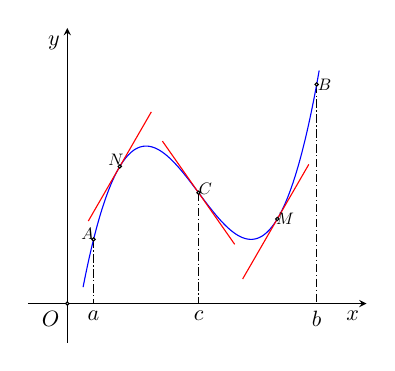
\begin{tikzpicture}
			\def\hsf(#1){((#1)^3-5*(#1)^2+7*(#1)-1}%ham so f
			\draw[-stealth,very thin](-.5,0)--(3.8,0)node[below left,scale=.8]{$x$};%truc Ox
			\draw[-stealth,very thin](0,-.5)--(0,3.5) node[below left,scale=.8]{$y$};%truc Oy
			\draw[fill=white](0,0)circle(.6pt)node[below left,scale=.8]{$O$};%goc toa do O
			\path (1/3,{\hsf(1/3)})coordinate(A) (19/6,{\hsf(19/6)})coordinate(B) (5/3,{\hsf(5/3)})coordinate(C)
			(8/3,{\hsf(8/3)})coordinate(M) (2/3,{\hsf(2/3)})coordinate(N);
			\draw[color=black,densely dash dot, thin] (A)--(1/3,0)node[below ,scale=.8] {$a$} (B)--(19/6,0)node[below ,scale=.8] {$b$} (C)--(5/3,0)node[below ,scale=.8] {$c$};
			\draw[blue,smooth,samples=100] plot[domain=.2:3.2](\x,{\hsf(\x)});
			\draw[red] (C)--+(125:.8)(C)--+(-55:.8) 
			(N)--+(60:.8)(N)--+(-120:.8) 
			(M)--+(60:.8)(M)--+(-120:.88);
			\foreach \p/\g in{A/140,B/0,C/30,M/0,N/120} \draw[fill=white](\p)circle(.6pt)+(\g:.1)node[scale=.6]{$\p$};
		\end{tikzpicture}
	\end{center}
	Điểm phân cách giữa cung lồi và cung lõm được gọi là \textbf{\color{diendantoanhoc}\itshape điểm uốn}. Điểm $C$ của đồ thị trong hình là điểm uốn.
	\vskip 0.1cm
	Nói cách khác thì: 
	Nếu hàm số $y=f(x)$ có đạo hàm trên khoảng $I$ ta nói rằng
	\vskip 0.1cm
	$a)$ Đồ thị ($C$) của hàm số $y = f(x)$ lồi trên khoảng $I$ nếu tiếp tuyến của ($C$) tại mỗi điểm của nó đều nằm phía trên đồ thị.
	\vskip 0.1cm
	$b)$ Đồ thị ($C$) của hàm số $ y = f(x)$ lõm trên khoảng $I$ nếu tiếp tuyến của nó tại mỗi điểm của nó đều nằm phía dưới đồ thị.
	\vskip 0.1cm
	\textbf{\color{diendantoanhoc}Nhận xét:} Một hàm được gọi là lồi (tương ứng, lõm) nếu đồ thị của nó là lồi (tương ứng, lõm). Đồ thị hàm lồi có hình dạng giống như một cái mũ $\cap $ còn của hàm lõm thì có hình dạng giống như một cái cốc  $\cup $.
	\vskip 0.1cm
	\textbf{\color{diendantoanhoc}$\pmb{2.}$ Dấu hiệu lồi, lõm và điểm uốn của đồ thị}
	\vskip 0.1cm
	Ta thừa nhận dấu hiệu lồi, lõm sau đây:
	\vskip 0.1cm
	\textbf{\color{diendantoanhoc}Định lý:} Cho hàm số $y = f(x)$ có đạo hàm đến cấp hai trên khoảng $I$.
	\vskip 0.1cm
	$1)$ Nếu $f "(x)< 0$ với mọi $x\in I$ thì đồ thị của hàm số \textbf{\color{diendantoanhoc}\itshape lồi} trên khoảng đó. 
	\vskip 0.1cm
	$2)$ Nếu $f "(x)> 0$ với mọi $x\in I$ thì đồ thị của hàm số  \textbf{\color{diendantoanhoc}\itshape lõm} trên khoảng đó.
	\vskip 0.1cm
	\textbf{\color{diendantoanhoc}Định lý:} Giả sử hàm số $y = f(x)$ có đạo hàm cấp hai trên một khoảng $I$ chứa điểm $ x _0$. Nếu $f"(x_0) = 0$ và $f"(x) $ đổi dấu khi $x$ qua điểm $x_0$ thì $U(x_0;f(x_0))$ là một điểm uốn của đồ thị hàm số $y = f(x)$.
	\vskip 0.1cm
	Tại điểm uốn tiếp tuyến đi xuyên qua đồ thị.
	\vskip 0.1cm
	\textbf{\color{diendantoanhoc}$\pmb{3.}$ Điều kiện để hai đường cong tiếp xúc nhau}
	\vskip 0.1cm
	Điều kiện để hai đường cong $y= f(x)$ và $y=g(x) $ tiếp xúc nhau là hệ phương trình sau có nghiệm và nghiệm của hệ là hoành độ giao điểm của hai đường cong đó \begin{align*}
		\begin{cases}f(x)=g(x)\\ f'(x)=g'(x)\end{cases}\tag{$*$}
	\end{align*}
	Vậy, đồ thị của $f$ và $g$ tiếp xúc nhau tại $x_0$ khi và chỉ khi $x_0$ là nghiệm của hệ ($*$).
	\vskip 0.1cm
	Thêm vào đó, nếu hai đường cong $y=f(x)$ và $y=g(x)$ có tính lồi lõm trái ngược nhau, ngoài ra có chung nhau tiếp tuyến thì khi đó phương trình $f(x)=g(x)$ có nghiệm duy nhất.
	\begin{center}
		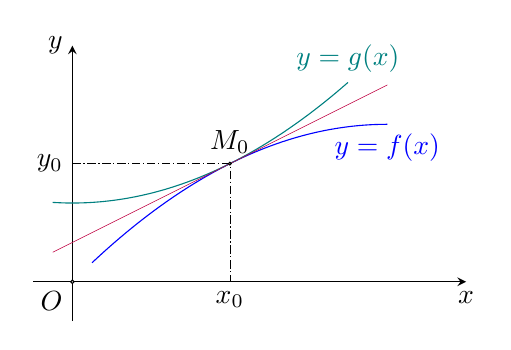
\begin{tikzpicture}
			\def\hsf(#1){-.125*(#1)^2+(#1)}%ham so f
			\def\hsg(#1){.125*(#1)^2+1}%ham so g
			\draw[-stealth] (-.5,0)--(5,0)node[below]{$x$};
			\draw[-stealth] (0,-.5)--(0,3)node[left]{$y$};
			\draw[fill=white](0,0)circle(.6pt)node[below left]{$O$};
			\draw[densely dash dot,very thin] (0,3/2)node[left]{$y_0$}-|(2,0) node[below]{$x_0$};
			\draw[smooth,blue]plot[domain=.25:4](\x,{\hsf(\x)}) node[below]{$y=f(x)$};
			\draw[smooth,teal]plot[domain=-.25:3.5](\x,{\hsg(\x)}) node[above]{$y=g(x)$};
			\draw[smooth,very thin,purple]plot[domain=-.25:4](\x,{.5*\x+1/2});
			\draw[fill=white](2,3/2)circle(.5pt)node[above]{$M_0$};
		\end{tikzpicture}
	\end{center}
	Cần phải chú ý rằng nhiều tài liệu trong và ngoài nước hiện nay định nghĩa về tính lồi (convex), lõm (concave) của đồ thị hàm số khác như đã nêu ở trên. Cụ thể là hàm lồi trong bài viết này được gọi là hàm lõm trong một số tài liệu, còn hàm lõm trong bài viết này thì lại được họ gọi là hàm lồi. 
	\vskip 0.1cm
	\textit{\textbf{\color{diendantoanhoc}Ta sẽ vận dụng những tính chất và nhận xét trên để ứng dụng trong việc giải một số bài toán về phương trình, bất phương trình, đây cũng chính là cở sở của phương pháp tiếp tuyến trên}}.
	\vskip 0.1cm
	Trong bài viết này chúng ta viết tắt VT cho vế trái, VP cho vế phải.
	Việc kiểm tra dấu hiệu lồi, lõm của hàm số bằng cách tính đạo hàm cấp hai trong một số ví dụ sẽ được dành cho bạn đọc.
	\vskip 0.1cm
	\textbf{\color{diendantoanhoc}$\pmb{4.}$ Các ví dụ}
	\vskip 0.1cm
	\textbf{\color{diendantoanhoc}Ví dụ $\pmb{1.}$} Giải phương trình
	\begin{align*}
		x^2-2x+5=\sqrt{x+3}+\sqrt{5-x}.
	\end{align*}
	\textit{Lời giải.} Điều kiện $-3\leq x\leq 5$. Vế trái là hàm lõm còn vế phải là hàm lồi (bạn đọc tự kiểm tra), chúng có chung tiếp tuyến tại $(1;4)$. Vậy $x=1$ là nghiệm duy nhất của phương trình.
	\vskip 0.1cm
	\textbf{\color{diendantoanhoc}Nhận xét:} Bài tập kiểu như trên rất quen thuộc với nhiều bạn đọc, phương pháp thường dùng là đánh giá bất đẳng thức. Ở đây, chúng ta sử dụng tiếp cận khác thông qua tiếp tuyến.
	\vskip 0.1cm
	Ta sẽ đến với những ví dụ khác, đòi hỏi đến cả kỹ năng nhẩm nghiệm.
	\vskip 0.1cm
	\textbf{\color{diendantoanhoc}Ví dụ $\pmb{2.}$} Giải phương trình
	\begin{align*}
		\sqrt[6]{6x-5}=\dfrac{x^{7}}{8x^{2}-10x+3}.
	\end{align*}
	\textit{Lời giải.} Điều kiện $x\ge \frac{5}{6}$. Với $x\ge \frac{5}{6}$ thì $VT$ là hàm lồi, liên tục, vì vậy đồ thị hàm số nằm dưới tiếp tuyến của nó tại điểm $x=1$ là $y=x+1$.
	Với $x\ge\frac{5}{6}$ thì $VP$ là hàm lõm, liên tục, vì vậy đồ thị hàm số nằm trên tiếp tuyến của nó tại điểm $x=1$ là $y=x+1$.
	\vskip 0.1cm
	Vậy $x=1$ là nghiệm duy nhất của phương trình. 
	\vskip 0.1cm
	\textbf{\color{diendantoanhoc}Ví dụ $\pmb{3.}$} Cho hai hàm số $f(x)$ và $g(x)$ được xác định như sau: $f(x)=\sqrt{13x^{2} - 6x + 10 } + \sqrt{5x^{2} -13x + \frac{17}{2}} + \sqrt{17x^{2} - 48x + 36} $ và $g(x)= \dfrac{1}{2}(36x - 8x^{2} - 21)$.
	\vskip 0.1cm
	Giải phương trình $f(x)=g(x)$.
	\vskip 0.1cm
	\textit{Lời giải.} Điều kiện $x\in \mathbb R$. Đặt $h(x)=f(x)-g(x)$\\ Không khó để chỉ ra $h(x)$ là hàm lõm, liên tục. Nhận thấy $h(\dfrac{3}{2})=0$ và $h'(\dfrac 32)=0$ , do đó đồ thị hàm số tiếp xúc với trục hoành tại điểm $x=\dfrac{3}{2}$.
	\vskip 0.1cm
	Vậy $x=\dfrac{3}{2}$ là nghiệm duy nhất của phương trình của bài toán.
	\vskip 0.1cm
	\textbf{\color{diendantoanhoc}Ví dụ $\pmb{4.}$} Giải phương trình
	\begin{align*}
		x\sqrt{x^2\!+\!6}\!+\!(x\!+\!1)\sqrt{x^2\!+\!2x\!+\!7}\!=\!\dfrac{13}{5}(2x\!+\!1)
	\end{align*}
	\textit{Lời giải.}  Điều kiện $x\in\mathbb R$. Đặt $g(x)=x\sqrt{x^2+6}$ và $f(x)=g(x+1)+g(x)$.
	\vskip 0.1cm
	Ta dễ kiểm tra thấy rằng:
	\vskip 0.1cm
	$a)$ $g(x)$ là hàm lẻ và $g''(x)$ cũng là hàm lẻ; hơn nữa ta cũng có $f(-\dfrac 12)=f''(-\dfrac 12)=0$.
	\vskip 0.1cm
	$b)$ $g(x)$ và $g''(x)$ là hàm đồng biến, suy ra $f(x)$ và $f''(x)$ cũng là hàm đồng biến.
	\vskip 0.1cm
	$c)$ Tiếp tuyến với đồ thị của hàm số  $f(x)$ tại $x=-\dfrac 12$ là $y=\dfrac{13}5(2x+1)$.
	\vskip 0.1cm
	Vậy đồ thị hàm số $f(x)$ nằm dưới tiếp tuyến của nó khi $x<-\dfrac 12$ và đồ thị hàm số $f(x)$ nằm trên tiếp tuyến của nó khi $x>-\dfrac 12$.
	\vskip 0.1cm
	Vậy $x=-\dfrac{1}{2}$ là nghiệm duy nhất của phương trình.
	\vskip 0.1cm
	\textbf{\color{diendantoanhoc}Chú ý:} Ở ví dụ này nghiệm của phương trình chính là hoành độ điểm uốn của đồ thị.
	\vskip 0.1cm
	\textbf{\color{diendantoanhoc}Ví dụ $\pmb{5.}$} Giải phương trình
	\begin{align*}
		&3\left(x^{3}+\frac{x}{\sqrt{\left(1+x^{2} \right)^{3}}} \right)+2\\
		=\,\,&\sqrt{\left(1+x \right)^{3}}+\sqrt{\left(1-x \right)^{3}}.
	\end{align*}
	\textit{Lời giải.}  Điều kiện xác định $x\in[-1;1]$. Nhận xét rằng $x=0$ là một nghiệm của phương trình. Đặt $f(x)=x+(1+x)^{-\frac 32}$ và $g(x)=\dfrac{(1+x)^{\frac 32}+(1-x)^{\frac 32}-2}x$.
	\vskip 0.1cm
	Giả sử $x\ne 0$. Phương trình đã cho có thể được viết lại thành $3f(x^2)=g(x)$.
	\vskip 0.1cm
	Chú ý rằng:
	\vskip 0.1cm
	Một mặt, $g(x)$ là hàm lẻ, nhận giá trị âm trên $[-1;0)$ và dương trên $(0, 1]$ và đồng biến trên mỗi khoảng này (bạn đọc tự kiểm tra), nên $g(x)\le g(1)=2\sqrt 2-1 <1$ với mọi $0\ne  x\in[-1,1]$.
	\vskip 0.1cm
	Mặt khác, $f(x)$ là hàm lõm trên $[0,1]$ (bạn đọc tự kiểm tra), vì vậy đồ thị hàm số nằm trên tiếp tuyến của nó tại điểm $x=0$ : $f(x)\ge 1-\frac x2\ge \frac 12$.
	\vskip 0.1cm
	Vậy $f(x^2)\ge \frac 12$, suy ra $3f(x^2)\ge \frac 32 > 1\ge g(x)$, do đó phương trình không còn nghiệm nào nữa. 
	\vskip 0.1cm
	Vậy $x=0$ là nghiệm duy nhất của phương trình đã cho.
	\vskip 0.1cm
	\textbf{\color{diendantoanhoc}Ví dụ $\pmb{6.}$} Cho số lẻ $n>1$. Giải phương trình
	\begin{align*}
		n^{x^n-1}+n^{\frac{1}{x}}=n+1.
	\end{align*}
	\textit{Lời giải.} Điều kiện xác định: $x \neq 0$. 
	Nếu $x<0$ thì VT$<2<$VP nên trường hợp này phương trình vô nghiệm.
	\vskip 0.1cm
	Xét trường hợp $x>0$. Xét hàm số $f(x):\mathbb R^+\to \mathbb R$ xác định bởi:
	\begin{align*}
		f(x)=n^{x^n-1}+n^{\frac 1x}-n-1
	\end{align*}
	Ta lần lượt có:
	\begin{align*}
		f'(x)=&\,n(\ln n)x^{n-1}n^{x^n-1}-\frac {\ln n}{x^2}n^{\frac 1x}.\\
		f''(x)=&\,n(\ln n)\left(n(\ln n)x^{2n-2}+(n-1)x^{n-2}\right)\\
		&\times n^{x^n-1}+\ln n\left(\frac {\ln n}{x^4}+\frac 2{x^3}\right)n^{\frac 1x}.
	\end{align*}
	Nhận thấy rằng $f(1)=f'(1)=0$, do đó tiếp tuyến của hàm số $f(x)$ tại điểm $x=1$ là trục hoành.
	\vskip 0.1cm 
	Vì $f(x)$ là hàm lõm và liên tục ($f''(x)>0$) do đó $x=1$ là nghiệm duy nhất của phương trình. 
	\vskip 0.1cm
	\textbf{\color{diendantoanhoc}Ví dụ $\pmb{7.}$} Giải bất phương trình
	\begin{align*}
		45x^3\!-\!17x^2\!-\!37x\!+\!25\!\ge\! 4\sqrt{\!\!(x\!+\!1)(5x\!-\!3)^3}.
	\end{align*}
	\textit{Lời giải.} Bất phương trình đã cho được viết lại thành 
	\begin{align*}
		(x\!+\!1\!)(45x^2\!-\!62x\!+\!25)\!\ge\! 4\sqrt{\!\!(x\!+\!1\!)(5x\!-\!3)^3}.
	\end{align*}
	Nhận thấy rằng một nghiệm là $x=-1$; các nghiệm khác phải thỏa mãn $x>-1$ (trái lại thì VT$<0\le$ VP), và thật ra $x\ge\frac 35$ (trái lại thì VP không xác định).
	\vskip 0.1cm
	Khi đó (với điều kiện $x\ge\frac 35$) bất phương trình trở thành
	\begin{align*}
		45x^2-62x+25\ge 4(5x-3)\sqrt{\dfrac{5x-3}{x+1}}.
	\end{align*}
	Nhận thấy một nghiệm thứ hai là $x=\frac 35$. Vậy với $x>\frac 35$ bất phương trình trở thành
	\begin{align*}
		\dfrac{45x^2-62x+25}{4(5x-3)}\ge \sqrt{\dfrac{5x-3}{x+1}}.
	\end{align*}
	VT là hàm lõm (bạn đọc tự kiểm tra) với tiếp tuyến $y=x$ tại $x=1$, VP là hàm lồi (bạn đọc tự kiểm tra) với tiếp tuyến $y=x$ tại $x=1$. Vậy đồ thị hàm số VT luôn nằm trên đồ thị của VP,  do đó bất phương trình luôn đúng.
	\vskip 0.1cm
	Vậy nghiệm của bất phương trình là: \linebreak $x\in\{-1\}\cup\left[\frac 35,+\infty\right)$
	\vskip 0.1cm
	\textbf{\color{diendantoanhoc}$\pmb{5.}$ Bài tập đề nghị}
	\vskip 0.1cm
	\textbf{\color{diendantoanhoc}Bài $\pmb{1.}$} Giải các phương trình sau trên tập số thực
	\vskip 0.1cm
	$a)$  $\sqrt[4]{x}=\frac{3}{8}+2x$.
	\vskip 0.1cm
	$b)$ $8x^2+\sqrt{\frac{1}{x}}=\frac{5}{2}.$
	\vskip 0.1cm
	$c)$ $16x^4+5=6\sqrt[3]{4x^3+x}.$
	\vskip 0.1cm
	$d)$ $ 2\sqrt[4]{\dfrac{x^{2}}{3}+4}=1+\sqrt{\dfrac{3x}{2}}.$
	\vskip 0.1cm
	$e)$ $x^2+2x+4=3\sqrt{x^3+4x}.$
	\vskip 0.1cm
	$f)$ $2^{x^2}+3^{x^2}+4^{x^2}+5^{x^2}=4^{1-x^2}.$
	\vskip 0.1cm
	$g)$ $x^2+x = (6x-x^2-2)\sqrt{x-1}.$
	\vskip 0.1cm
	$h)$ $2x^2-11x+21-3\sqrt[3]{4x-4}=0.$
	\vskip 0.1cm
	$i)$ $x^{3}+x^{2}-15x+30=4\sqrt[4]{27(x+1)}.$
	\vskip 0.1cm
	$j)$ $2\sqrt[4]{27x^2+24x+\frac{28}{3}}=1+\sqrt{\frac{27x}{2}+6}.$
	\vskip 0.1cm
	$k)$ $\sqrt{x^2+x-1}+\sqrt{x-x^2+1}=x^2-x+2.$
	\vskip 0.1cm
	$l)$ $x^2-2x+3=\sqrt{2x^2-x}+\sqrt{1+3x-3x^2}.$
	\vskip 0.1cm
	$m)$ $\sqrt{x^2+x+19}+\sqrt{7x^2+22x+28}$\\
	$\quad\,\,+\sqrt{13x^2+43x+37}=3\sqrt{3}(x+3)$.
	\vskip 0.1cm
	$n)$ $\log_2 \dfrac{2x+1}{4x} = \log_{x} \dfrac{2x+1}{2}.$\\
	\vskip 0.1cm
	\textbf{\color{diendantoanhoc}Bài $\pmb{2.}$} Tồn tại hay không các cặp số thực âm $(x,y)$ thoả mãn phương trình \linebreak$x2^y+y2^{-x}=x+y$?
	\vskip 0.1cm
	\textbf{\color{diendantoanhoc}Bài $\pmb{3.}$} Tìm tất cả các số thực $a$ sao cho bất phương trình $a^x\geq 1+x\log _{11}12$ đúng với mọi số thực $x$.
	\vskip 0.1cm
	\textbf{\color{diendantoanhoc}Tài liệu tham khảo}
	\vskip 0.1cm
	[$1$] Ngô Thúc Lanh (chủ biên), {\it Giải tích $12$ }(SGK), Nhà xuất bản Giáo Dục ($2006$).
	\vskip 0.1cm
	[$2$] Nguyễn Huy Đoan (chủ biên), {\it Giải tích $12$ nâng cao} (SGK), Nhà xuất bản Giáo Dục ($2008$).
	\vskip 0.1cm
	[$3$] Phan Đức Chính (chủ biên), {\it Một số phương pháp chọn lọc giải các bài toán sơ cấp (Tập $2$)}, Nhà xuất bản Đại học Quốc gia Hà Nội ($2003$). 
	\vskip 0.1cm
	[$4$] Nguyễn Quang Nam, {\it Kỹ thuật tạo nhân tử kép}, Tạp chí Toán học và Tuổi trẻ, Nhà xuất bản Giáo Dục (Số $511$, tháng $1/2020)$.
	\vskip 0.1cm
	[$5$]~\url{https://artofproblemsolving.com/com} \url{munity}
	\end{multicols}
%\newpage

%
%	\setcounter{figure}{0}
%	\thispagestyle{doisongtoanhocnone}
\pagestyle{doisongtoanhoc}
\everymath{\color{doisongtoanhoc}}
\graphicspath{{../doisongtoanhoc/pic/}}
%\blfootnote{$^1$\color{doisongtoanhoc}Trung tâm Thông tin -- Tư liệu, Viện Hàn lâm Khoa học và Công nghệ Việt Nam.}
\begingroup
\AddToShipoutPicture*{\put(0,616){\includegraphics[width=19.3cm]{../bannerdoisong}}}
\AddToShipoutPicture*{\put(43,527){\includegraphics[scale=0.95]{../tieude.pdf}}}\centering
\endgroup

\vspace*{185pt}


\begin{multicols}{2}	
	Đại hội Toán học Quốc tế (International Congress of Mathematicians, sau đây sẽ viết tắt là ICM) là sự kiện khoa học quan trọng hàng đầu của các nhà toán học trên thế giới. Nhiều người trong chúng ta đã quen thuộc với Kỳ thi Olympic Toán quốc tế (IMO). Vậy ICM có gì giống và khác với IMO? Mục đích của ICM là gì? Những hoạt động chính tại một kỳ ICM là gì? ICM $2022$ có những dấu ấn gì đặc biệt? Chúng tôi sẽ thử giải đáp các câu hỏi này.
	\vskip 0.1cm
	$\pmb{1.}$ \textbf{\color{doisongtoanhoc}ICM có gì giống và khác với IMO?}
	\vskip 0.1cm
	Cũng giống như IMO, ICM là một hoạt động cộng đồng hướng đến mục tiêu phát triển sự quan tâm đến toán học. Có lịch sử lâu đời hơn IMO một chút, ICM đầu tiên được tổ chức từ năm $1897$ tại Z\"urich, Thụy Sĩ, nhưng trong khi IMO được tổ chức hầu như hằng năm, thì ICM được tổ chức bốn năm một lần. Nếu IMO tập trung vào việc giải các bài toán, thì ICM hướng đến trình bày những thành tựu nghiên cứu toán học đáng kể nhất gần đây. Không có sự khác biệt đáng kể giữa nghiên cứu toán học và giải các bài toán Olympic, vì cả hai công việc đều đòi hỏi kỹ năng giải quyết vấn đề. Chúng ta biết rằng có những bài toán mở nổi tiếng trong toán học, như  định lý lớn Fermat (là bài toán mở đến trước $1994$), giả thuyết về số nguyên tố sinh đôi, hay giả thuyết Riemann (cả hai hiện vẫn chưa được giải quyết). Những tiến bộ về các bài toán mở nổi tiếng, nếu có, cũng là một điểm nhấn quan trọng của những kỳ ICM. Nhưng so với việc thi olympic, có thể nói các nhà toán học có nhiều tự do hơn trong việc làm nghiên cứu của mình, họ không nhất thiết phải làm việc với một vấn đề có sẵn. Có những nhà toán học lớn theo đuổi một vấn đề  hàng năm, thậm chí hàng chục năm trời. Việc một nhà số học ngồi nghe một bài giảng hình học đại số, hay một nhà đại số dự một bài giảng vật lý toán, để mở mang kiến thức, cũng là một việc thường xảy ra và được ICM khuyến khích.
	\vskip 0.1cm
	$\pmb{2.}$ \textbf{\color{doisongtoanhoc}Vì sao cần tổ chức ICM?}
	\vskip 0.1cm
	Mục đích chính của ICM là để tạo điều kiện cho các nhà toán học từ khắp nơi trên thế giới gặp gỡ những chuyên gia hàng đầu, và để tôn vinh những thành tựu toán học nổi bật nhất gần đây.
	\vskip 0.1cm
	Các nhà toán học gặp gỡ nhau? Chẳng phải các nhà toán học chỉ cần có giấy bút (và máy tính) để làm việc đó sao? Đúng là phần lớn các nhà toán học  có thiên hướng lý thuyết,  không cần nhiều trang thiết bị để làm việc. Nhưng ngoài giấy bút và máy tính, họ cũng thường cần một người đồng nghiệp ăn ý để thử nghiệm những ý tưởng chợt đến, tranh cãi về một chứng minh trong một bài báo, hay đơn giản tán gẫu về trận bóng tối qua. 
	\vskip 0.1cm
	Như bất cứ ngành khoa học có truyền thống nào, toán học ngày càng đa dạng hóa và chuyên môn hóa cao độ, với rất nhiều phân ngành khác nhau. ICM đầu tiên năm $1897$ chỉ có năm tiểu ban, mỗi tiểu ban phụ trách một chuyên môn, gồm có số học và đại số, giải tích và lý thuyết hàm, hình học, cơ học và vật lý toán, lịch sử và thư mục toán học. Nửa thế kỷ sau, ICM $1958$ mới có tám tiểu ban\footnote{\color{doisongtoanhoc}Xem Guillermo P. Curbera, \emph{Mathematicians of the World, Unite!}, Wellesley, Massachusetts: A.K. Peters, Ltd ($2009$), trang $14$ và $141$.}. Đến ICM $2022$, ta có đến hai mươi tiểu ban: logic, đại số, hình học đại số và hình học phức, tôpô, lý thuyết Lie và các mở rộng, giải tích, động lực học, phương trình vi phân, vật lý toán... Mỗi tiểu ban ngày nay lại có nhiều tiểu mục nhỏ hơn, ví dụ tiểu ban đại số có bốn tiểu mục.  Ngay từ ICM năm $1908$ ở Rome, Poincar\'e đã nhận ra: ``Khi một khoa học càng phát triển, ta càng khó nắm bắt được toàn bộ khoa học đó. Từ đó người ta phải chia nhỏ khoa học ấy ra nhiều phần, và bằng lòng với việc chỉ quan tâm tới đúng một trong các phần đó, nói cách khác là phải chuyên môn hóa. Chuyên môn hóa quá sâu sẽ làm cản trở nghiêm trọng đến tiến bộ chung của khoa học (...) Chính nhờ những tương tác bất ngờ giữa các hướng nghiên cứu khác nhau mà khoa học mới có thể phát triển."\footnote{\color{doisongtoanhoc}``In proportion as the science develops, it becomes more difficult to take it in its entirety. Then an attempt is made to
		cut it in pieces and to be satisfied with one of these pieces -- in
		a word, to specialize. Too great a movement in this direction
		would constitute a serious obstacle to the progress of science. As I have said, it is by unexpected concurrences
		between its different parts that it can make progress." Xem The Mathematical Intelligencer, Tập $34$, số $2$ ($2012$), trang $15-29$.} Nhà toán học nổi tiếng Hoàng Tụy ($1927-2019$) sinh thời thường cảnh báo về nguy cơ của chủ nghĩa tỉnh lẻ, khi một nhà khoa học làm việc trong tinh thần bế quan tỏa cảng và khiến bản thân thui chột. Gặp gỡ và tương tác với những chuyên gia hàng đầu tại những sự kiện lớn như ICM là cách giúp một nhà khoa học ``mở con mắt hướng ra những bờ cõi khoa học nơi những người khác đang chiếm cứ, và buộc ta phải so sánh thành tựu của mình với họ, qua đó nhận ra ngôi làng mình đang sống nhỏ bé chừng nào", theo lời của Poincar\'e\footnote{\color{doisongtoanhoc}Tài liệu đã dẫn, trang $20$.}.
	\vskip 0.1cm
	$\pmb{3.}$ \textbf{\color{doisongtoanhoc}Hoạt động chính ở các ICM là gì?}
	\vskip 0.1cm
	Hoạt động chính của ICM là các bài giảng của các chuyên gia, và phần trao giải thưởng ghi nhận những thành tựu toán học cao nhất đã đạt được giữa hai kỳ đại hội. Các bài giảng của chuyên gia gồm hai loại là các bài giảng toàn thể (khoảng $20$ bài) và các bài giảng tiểu ban (khoảng 180 bài). Được đọc bài giảng tại một ICM là một vinh dự lớn, nếu ta biết rằng mỗi năm có khoảng gần một trăm nghìn công trình toán học được xuất bản trên các tạp chí chuyên ngành. Các giải thưởng được trao ở các kỳ ICM gần đây là huy chương Fields (cho nhà toán học trẻ xuất sắc), giải thưởng Nevanlinna (khía cạnh toán học trong tin học), giải Gauss (toán ứng dụng), huy chương Chern (những người có thành tựu toán học xuất chúng, không hạn chế tuổi tác), và giải Leelavati (phổ biến kiến thức và quảng bá toán học). Trong số này, huy chương Fields nói chung được coi là giải thưởng danh giá nhất.
	\vskip 0.1cm
	$\pmb{4.}$ \textbf{\color{doisongtoanhoc}Ai có thể giành được huy chương Fields?}
	\vskip 0.1cm
	Huy chương Fields được trao cho những nhà toán học dưới $40$ tuổi với thành tựụ xuất sắc và tiềm năng phát triển lớn. Nhìn vào những người đoạt huy chương Fields gần đây, ta thấy họ nói chung là những người tài năng, được đào tạo bài bản (có bằng tiến sĩ), và theo đuổi những lĩnh vực quan trọng hoặc những bài toán quan trọng trong một thời gian dài. Có lẽ cách chắc chắn nhất để \emph{không} giành được giải Fields là lao vào những bài toán nổi tiếng, nhiều người biết, như giả thuyết Collatz, hay giả thuyết Riemann, bằng tay không, không quan tâm đến việc tích lũy kiến thức và các kỹ thuật cơ bản dần dần. Những huy chương Fields, ngoài sự dũng cảm tấn công những vấn đề khó khăn, còn ghi dấu ấn cụ thể, thuyết phục với những bài báo với nhiều người đọc, được bình duyệt chặt chẽ, trên những tạp chí toán học uy tín. Thông thường họ đã có một công chúng rộng lớn, những ý tưởng của họ đã có ích lợi đáng kể cho công việc của nhiều người khác, \emph{trước khi} được vinh danh với huy chương Fields, chứ không phải ngược lại. Tất nhiên không có quy tắc chung cho những tài năng đặc biệt, họ thường  phá vỡ những quy tắc mà chúng ta coi như hiển nhiên.
	\vskip 0.1cm
	$\pmb{5.}$ \textbf{\color{doisongtoanhoc}Đại hội Toán học Quốc tế $2022$ có gì đặc biệt?}
	\vskip 0.1cm
	ICM $2022$ được tổ chức từ ngày mùng $6$ đến $14/7/2022$. Lễ trao các giải thưởng được tổ chức trực tiếp tại Helsinki, Phần Lan vào ngày $5/7$. Về hình thức, sau $125$ năm lịch sử, đây là lần đầu tiên chương trình khoa học của ICM được tổ chức theo hình thức trực tuyến. Tại ICM năm nay, huy chương Fields đã được trao cho Hugo Dominil--Copin (Pháp), June Huh (Hàn Quốc), James Maynard (Vương quốc Anh), và Maryna Viazovska (Ukraina). Đây đều là những tên tuổi hàng đầu của toán học đương đại, những người sẽ còn tiếp tục ảnh hưởng lâu dài đến toán học. Nếu bạn nghĩ một bài giảng toán học là đối cực của một tiểu thuyết hấp dẫn/một bộ phim hay? Mời bạn xem bài giảng hết sức sáng sủa với đoạn cao trào tuyệt vời của June Huh, một người làm toán (những bài toán không hề đơn giản!) với hồn thơ đặc biệt. Nếu bạn, sau khi sở hữu một cỗ máy tiêu diệt hàng loạt các loại bài toán khó muôn hình vạn trạng, nghĩ quảng bá toán học là một việc nhàm chán và không cần công phu gì? Mời bạn xem bài giảng của Nikolai Andreev (giải Leelavati $2022$) và trang mạng độc đáo của ông\footnote{\color{doisongtoanhoc}https://etudes.ru/}.
	\vskip 0.1cm
	Trong một thế giới còn rất nhiều xung đột và đối kháng, các kỳ ICM và Liên đoàn Toán học Quốc tế (IMU) hướng đến gắn kết con người bằng toán học và tinh thần quốc tế, vượt qua những giới hạn về tư tưởng, ngôn ngữ, văn hóa, mặc cảm thượng đẳng/mặc cảm thấp kém thường ám ảnh con người. Từ khi kỳ ICM đầu tiên được tổ chức đến nay, toán học đã gánh chung tác động của hai thế chiến, chiến tranh lạnh, kỳ thị và phân biệt đối xử, với những hoạt động khác của con người. Vượt qua những khó khăn đó, cộng đồng toán học đã tiếp tục đi tới với lý tưởng bình đẳng, nhân văn, và chủ nghĩa quốc tế, di sản to lớn của những nhà toán học hàng đầu trong quá khứ. Chúng ta hy vọng vào thành công trong tương lai của toán học và của những lý tưởng này.
\end{multicols}

%	\newpage

%	\setcounter{figure}{0}
%	\thispagestyle{toanhocvadoisongnone}
\pagestyle{toanhocvadoisong}
\everymath{\color{toanhocdoisong}}
\graphicspath{{../toanhocdoisong/pic/}}
\begingroup
\blfootnote{$^1$\color{toanhocdoisong}Viện Sinh thái và Môi trường Đông Dương.}
\AddToShipoutPicture*{\put(0,616){\includegraphics[width=19.3cm]{../bannertoanhocdoisong}}}
\AddToShipoutPicture*{\put(79,520){\includegraphics[scale=1]{../tieude.pdf}}}
\centering
\endgroup

\vspace*{190pt}

\begin{multicols}{2}
	Bài toán cây kim của Buffon vẫn luôn xuất hiện trong sách giáo khoa toán dưới dạng một phương pháp để tính số $\pi$. Trong bài này, chúng ta hãy cũng Pi tìm hiểu chi tiết về bài toán này cũng như một số ứng dụng thú vị của nó trong thực tiễn.
	
	\vskip 0.1cm
	\textbf{\color{toanhocdoisong}$\pmb{1.}$ Bài toán cây kim của Buffon}
	\begin{figure}[H]
		\vspace*{-5pt}
		\centering
		\captionsetup{labelformat= empty, justification=centering}
		\includegraphics[width=0.6\linewidth]{1}
		\caption{\small\textit{\color{toanhocdoisong}Georges--Louis Leclerc, Comte de Buffon $(1707-1788)$.}}
		\vspace*{-10pt}
	\end{figure}
	Nhà toán học Pháp thế kỉ $18$, Georges Louis Leclerc, được phong Bá tước tại vùng có một ngôi làng tên Buffon nên ông còn có danh hiệu Comte de Buffon (Bá tước Buffon). Do đó các tài liệu thường gọi tắt là Buffon. Bài toán nổi tiếng mang tên ông có nội dung như sau:
	\vskip 0.1cm
	``Trên một tờ giấy với các đường kẻ cách đều nhau khoảng cách $d$, thả ngẫu nhiên một cây kim chiều dài $l$ $(d>l)$, hãy tìm xác suất để cây kim cắt một đường nằm ngang trên trang giấy".
	\begin{figure}[H]
		\vspace*{-5pt}
		\centering
		\captionsetup{labelformat= empty, justification=centering}
		\includegraphics[width=0.95\linewidth]{2}
		\caption{\small\textit{\color{toanhocdoisong}Hình $1$. Minh họa bài toán cây kim của Buffon.}}
		\vspace*{-10pt}
	\end{figure}
	Chúng ta hãy xét một lời giải không sử dụng tích phân được E. Barbier đưa ra năm $1860$.
	\vskip 0.1cm 
	Do $l<d$ nên chỉ có hai trường hợp xảy ra: cây kim cắt một đường kẻ và cây kim không đè lên đường kẻ nào; không tồn tại trường hợp cây kim cắt nhiều hơn một đường kẻ.
	\vskip 0.1cm
	Gọi $P(l)$ là xác suất để cây kim có độ dài $l$ cắt một đường kẻ khi được thả. Lấy một điểm bất kỳ trên cây kim chia nó thành hai đoạn thẳng độ dài $l_1$ và $l_2$. Ta có:
	\begin{align*}
		P(l)=P(l_1 )+P(l_2).
	\end{align*}
	Quan hệ trên có thể được mở rộng ra thành dạng $P(l)=n\cdot P(\dfrac{l}{n})$. Tức là xác suất để một cây kim cắt đường kẻ khi được thả sẽ bằng $n$ lần xác suất này của cây kim có độ dài bằng $\dfrac{1}{n}$ lần độ dài cây kim ban đầu.
	\vskip 0.1cm
	Do đó, $P(l)=c\cdot l$ với $c$ là một hằng số, $c=P(1)$ (khi $l=1$ và $d > 1$).
	\begin{figure}[H]
		\vspace*{-5pt}
		\centering
		\captionsetup{labelformat= empty, justification=centering}
		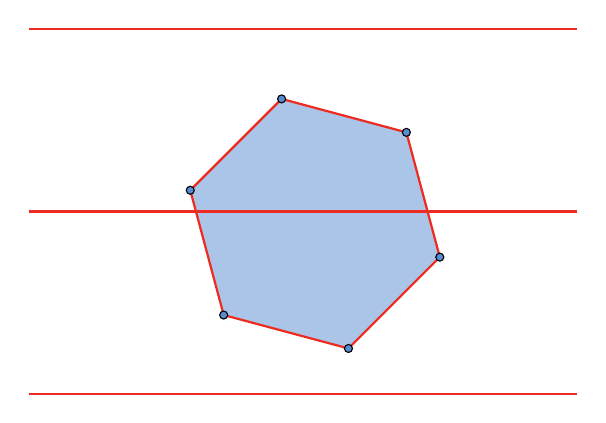
\begin{tikzpicture}[scale=0.58]
			\definecolor{qqqqff}{rgb}{0.,0.,1.}
			\definecolor{ududff}{rgb}{0.30196078431372547,0.30196078431372547,1.}
				\fill[line width=0.8pt,color=cackithi,fill=cackithi,fill opacity=0.5] (1.,3.) -- (3.,5.) -- (2.267949192431123,7.732050807568878) -- (-0.46410161513775494,8.464101615137755) -- (-2.4641016151377553,6.464101615137756) -- (-1.7320508075688794,3.7320508075688785) -- cycle;
				\draw [line width=0.8pt,color=toanhocdoisong] (1.,3.)-- (3.,5.);
				\draw [line width=0.8pt,color=toanhocdoisong] (3.,5.)-- (2.267949192431123,7.732050807568878);
				\draw [line width=0.8pt,color=toanhocdoisong] (2.267949192431123,7.732050807568878)-- (-0.46410161513775494,8.464101615137755);
				\draw [line width=0.8pt,color=toanhocdoisong] (-0.46410161513775494,8.464101615137755)-- (-2.4641016151377553,6.464101615137756);
				\draw [line width=0.8pt,color=toanhocdoisong] (-2.4641016151377553,6.464101615137756)-- (-1.7320508075688794,3.7320508075688785);
				\draw [line width=0.8pt,color=toanhocdoisong] (-1.7320508075688794,3.7320508075688785)-- (1.,3.);
				\draw [toanhocdoisong,line width=0.8pt] (-6.,6.)-- (6.,6.);
				\draw [toanhocdoisong,line width=0.8pt] (-6.,2.)-- (6.,2.);
				\draw [toanhocdoisong,line width=0.8pt] (-6.,10.)-- (6.,10.);
			
				\draw [fill=cackithi] (1.,3.) circle (2.5pt);
				\draw [fill=cackithi] (3.,5.) circle (2.5pt);
				\draw [fill=cackithi] (2.267949192431123,7.732050807568878) circle (2.5pt);
				\draw [fill=cackithi] (-0.46410161513775494,8.464101615137755) circle (2.5pt);
				\draw [fill=cackithi] (-2.4641016151377553,6.464101615137756) circle (2.5pt);
				\draw [fill=cackithi] (-1.7320508075688794,3.7320508075688785) circle (2.5pt);
		\end{tikzpicture}
		\caption{\small\textit{\color{toanhocdoisong}Hình $2$. Thả một đa giác cạnh $l$ lên tờ giấy với các đường kẻ ngang cách đều nhau.}}
		\vspace*{-10pt}
	\end{figure}
	Ta hãy tiếp tục xét một đa giác đều $N$ cạnh có độ dài mỗi cạnh bằng $l$ (Hình $2$). Ta đã biết ở trên rằng xác suất để mỗi cạnh của đa giác cắt một đường kẻ là $P(l)$. Đây cũng chính là giá trị kỳ vọng của số giao điểm của một cạnh với các đường kẻ, vì số giao điểm nói chung chỉ có thể là $0$ hoặc $1$ tương ứng với không cắt và cắt. Theo tính chất cộng tính của kỳ vọng, giá trị kỳ vọng của số giao điểm của đa giác với các đường kẻ khi thả lên tờ giấy là:
	\begin{align*}
		E &= \sum\nolimits_{i = 1}^N {P(l) = N \cdot } P(l) \\
		&= N \cdot c \cdot l = c \cdot L, \tag{$1$}
	\end{align*}
	với $L=N \cdot l$ là chu vi của đa giác đều.
	\vskip 0.1cm
	\columnbreak
	\PIbox{\textbf{\color{toanhocdoisong}Giá trị kỳ vọng}
		\vskip 0.1cm
		Trong một thí nghiệm ngẫu nhiên, nếu kết quả có giá trị $x_i$ có xác suất xảy ra là $p_i$ thì giá trị kỳ vọng của kết quả thu được được tính theo công thức:
		\setlength{\abovedisplayskip}{4pt}
		\setlength{\belowdisplayskip}{4pt}
		\begin{align*}
			E=x_1 p_1+x_2 p_2+ \cdots +x_n p_n.
		\end{align*}
		Ví dụ, với thí nghiệm gieo con xúc xắc, giá trị kỳ vọng của số chấm thu được là:
		\begin{align*}
			E=\frac{1}{6}\cdot 1 + \frac{1}{6} \cdot 2 + \cdots + \frac{1}{6}\cdot6 = 3{,5}.
		\end{align*}
		Chú ý rằng giá trị kỳ vọng có thể không trùng với một trong các giá trị có thể xảy ra. Theo định luật số lớn trong xác suất, với số lần thực hiện thí nghiệm càng lớn thì giá trị trung bình của các kết quả sẽ càng đến gần với giá trị kỳ vọng.}
	\vskip 0.1cm
	Mặt khác, nếu giữ chu vi $L$ của đa giác không đổi, khi $N \to \infty$, đa giác của ta sẽ trở thành một đường tròn có chu vi $L$ và bán kính $\dfrac{L}{2\pi}$.
	\vskip 0.1cm
	Để tính hệ số $c$, ta xét một trường hợp đặc biệt, khi đường tròn có đường kính đúng bằng khoảng cách $d$ giữa các dòng kẻ. Khi đó, ta có $L=\pi d$.
	\begin{figure}[H]
		\vspace*{-5pt}
		\centering
		\captionsetup{labelformat= empty, justification=centering}
		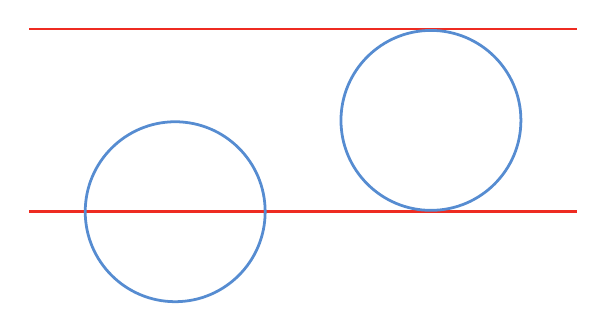
\begin{tikzpicture}[scale=0.58]
			\draw [toanhocdoisong, line width=1.pt] (-6.,6.)-- (6.,6.);
			\draw [toanhocdoisong, line width=1.pt] (-6.,10.)-- (6.,10.);
			\draw [cackithi, line width=1.pt] (2.8,8.) circle (1.97cm);
			\draw [cackithi, line width=1.pt] (-2.8,6.) circle (1.97cm);
		\end{tikzpicture}
		\caption{\small\textit{\color{toanhocdoisong}Hình $3$. Đường tròn có đường kính $d$ sẽ luôn cắt một đường kẻ tại hai điểm hoặc tiếp xúc hai đường kẻ.}}
		\vspace*{-10pt}
	\end{figure}
	Đường tròn có đường kính $d$ sẽ luôn cắt một đường kẻ tại $2$ giao điểm hoặc tiếp xúc với $2$ đường kẻ liên tiếp, do đó với đường tròn này $E=2$. Thay vào ($1$) ta có:
	\begin{align*}
		2=c\cdot\pi d
	\end{align*}
	hay $c = \dfrac{2}{\pi d}$.
	\vskip 0.1cm
	Vậy xác suất để một cây kim khi thả cắt đường nằm ngang trên giấy là 
	\begin{align*}
		P(l) = \frac{2l}{\pi d}. \tag{$2$}
	\end{align*}
	\begin{figure}[H]
		\vspace*{-5pt}
		\centering
		\captionsetup{labelformat= empty, justification=centering}
		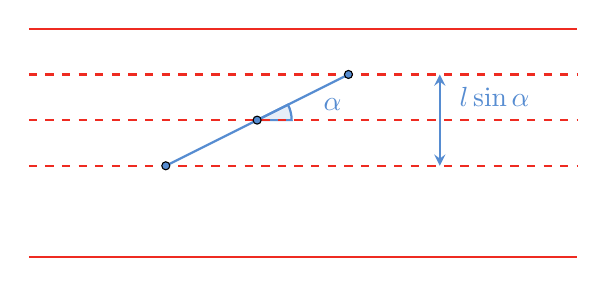
\begin{tikzpicture}[scale=0.58]
			\draw [shift={(-1.,8.)},line width=0.8pt,color=cackithi,fill=cackithi,fill opacity=0.15000000596046448] (0,0) -- (0.:0.7555063451882832) arc (0.:26.56505117707799:0.7555063451882832) -- cycle;
			\draw [toanhocdoisong,line width=0.8pt] (-6.,10.)-- (6.,10.);
			\draw [toanhocdoisong,dashed, line width=0.8pt] (-6.,9.)-- (6.,9.);
			\draw [toanhocdoisong,dashed, line width=0.8pt] (-6.,8.)-- (6.,8.);
			\draw [toanhocdoisong,dashed, line width=0.8pt] (-6.,7.)-- (6.,7.);
			\draw [toanhocdoisong, line width=0.8pt] (-6.,5.)-- (6.,5.);
			\draw [cackithi,line width=0.8pt] (-3.,7.)-- (1.,9.);
			\draw [fill=cackithi] (-3,7) circle (2.5pt);
			\draw [fill=cackithi] (1,9) circle (2.5pt);
			\draw [fill=cackithi] (-1,8) circle (2.5pt);
			\draw [cackithi,-stealth,line width=0.8pt] (3.,8.)-- (3.,9.);
			\draw [cackithi,-stealth,line width=0.8pt] (3.,8.)-- (3.,7.);
			
			\draw[color=cackithi] (0.65,8.347966297286694) node {$\color{cackithi}\alpha$};
			\draw[color=cackithi] (4.2,8.5) node {$\color{cackithi}l\sin\alpha$};
		\end{tikzpicture}
		\caption{\small\textit{\color{toanhocdoisong}Hình $4$. Chứng minh công thức $(2)$ sử dụng tích phân.}}
		\vspace*{-10pt}
	\end{figure}
	Ta cũng có thể thu được đáp án này bằng cách sử dụng tích phân. Cụ thể là ta xây dựng một mô hình xác suất cho vị trí rơi của cây kim. Gọi $\alpha$ $(0\le \alpha \le \dfrac{\pi}{2})$ là góc mà cây kim tạo với phương nằm ngang. Hình chiếu của nó theo phương vuông góc với các đường kẻ sẽ có độ dài $l\sin\alpha$, mà khoảng cách giữa hai đường kẻ là $d$, do đó xác suất để nó cắt một đường kẻ là $\dfrac{l\sin\alpha}{d}$. Coi phân bố của $\alpha$ là đều trên khoảng $[0,\dfrac{\pi}{2}]$, ta tính giá trị trung bình bằng cách lấy tích phân trên khoảng này rồi chia cho $\dfrac{\pi}{2}$ để thu được ($2$):
	\begin{align*}
		P(l) &= \frac{2}{\pi }\int_0^{\frac{\pi }{2}} {\frac{{l\sin \alpha }}{d}} d\alpha  = \frac{2}{\pi }\frac{l}{d}\left[ { - \cos \alpha } \right]|_0^{\frac{\pi }{2}}\\
		& = \frac{2}{\pi }\frac{l}{d}.
	\end{align*}
	Với cây kim có độ dài lớn hơn $d$, xác suất để nó cắt ít nhất một đường kẻ trong khoảng $\left[\arcsin\left(\dfrac{d}{l}, \dfrac{\pi}{2}\right)\right]$ sẽ luôn là $1$, do đó:
	\begin{align*}
		&P(l) \\
		= \,&\frac{2}{\pi }\left( {\int_0^{\arcsin \left( {\frac{d}{l}} \right)} {\frac{{l\sin \alpha }}{d} + } \int_{\arcsin \left( {\frac{d}{l}} \right)}^{\frac{\pi }{2}} {1d\alpha } } \right)\\
		=\,&1 \!\!+\!\! \frac{2}{\pi }\!\left( \!\!{\frac{l}{d}\!\!\left(\!\! {1 \!-\! \sqrt {\!\!1 \!-\! \frac{{{d^2}}}{{{l^2}}}} \!} \right) \!\!-\! \arcsin\! \frac{d}{l}}\! \right)\!\!.\tag{$3$}
	\end{align*}
	Bài toán này cũng được Laplace mở rộng cho trường hợp lưới trên tờ giấy là lưới chữ nhật và  tính xác suất để cây kim không cắt một đường kẻ dọc hay ngang nào. 
	\vskip 0.1cm
	Cũng chính Laplace đã đề xuất sử dụng thí nghiệm này để tính giá trị của số $\pi$. Đây cũng là khía cạnh được biết đến nhiều nhất về bài toán cây kim của Buffon. Thật vậy, nếu trong $M$ lần thả cây kim, ta thu được $m$ lần mà nó cắt một đường kẻ, công thức ($2$) cho ta:
	\begin{align*}
		\pi = \frac{2l}{d\cdot\left(\frac{m}{M}\right)},
	\end{align*}
	với $\dfrac{m}{M}$ là xác suất thực nghiệm của sự kiện cây kim cắt một đường kẻ.
	\vskip 0.1cm
	Đề xuất này của Laplace rất gần với phương pháp Monte Carlo của hơn một thế kỉ sau. Tuy vậy, về mặt thực tế, nó gập phải một số vấn đề. Nhiều thí nghiệm được tiến hành và cho kết quả của $\pi$ không quá chính xác: $3{,}1596$; $3{,}1553$; $3{,}137$.
	\vskip 0.1cm 
	Năm $1901$, Lazzarini công bố giá trị $3{,}1415929$ cho $3408$ lần thả cây kim, một giá trị khá chính xác (so với giá trị đã biết hiện nay, thì chỉ có chữ số cuối là không đúng). Tuy vậy, một số nghiên cứu đã chỉ ra kết quả này hầu như là ngụy tạo. Theo các lí thuyết về ước lượng tham số, để có độ chính xác đến $6$ chữ số sau dấu phẩy, cần phải tiến hành thí nghiệm trên $1{,}34×10^{14}$ lần chứ không phải vài nghìn lần. Đồng thời, số liệu của Lazzarini sử dụng phân số $\dfrac{355}{113}$, một số hữu tỉ được biết là một xấp xỉ tốt cho $\pi$. 
	\vskip 0.1cm
	Ngay cả với máy tính điện tử thì việc ước lượng $\pi$ bằng cách sử dụng thí nghiệm Buffon cũng không đạt được độ chính xác quá cao do việc làm tròn số trên máy tính. Đồng thời, các chữ số của $\pi$ cũng có thể được tính toán một cách chính xác hơn bởi các phương pháp khác.
	\vskip 0.1cm
	Tuy vậy, bài toán cây kim của Buffon có một ý nghĩa quan trọng trong lịch sử toán học bởi sự liên hệ giữa xác suất và hình học. Đây là một hướng tiếp cận mới khác với hướng tiếp cận xác suất sử dụng tổ hợp như truyền thống.
	\vskip 0.1cm
	\textbf{\color{toanhocdoisong}Bài tập}
	\vskip 0.1cm
	$1$. Chứng minh rằng khi cây kim vô cùng dài thì một cách hầu chắc chắn nó sẽ luôn cắt ít nhất một đường kẻ, tức là biểu thức trong ($3$) có giới hạn là $1$ khi $l\to \infty$.
	\vskip 0.1cm
	$2$. Trên tờ giấy với các đường kẻ ngang cách nhau khoảng $d$, thả ngẫu nhiên một đường tròn với bán kính $r < \dfrac{d}{2}$. Hãy tính xác suất để đường tròn cắt và không cắt các đường kẻ.
	\vskip 0.1cm
	$3$. Tương tự bài trên nhưng thả một hình vuông có cạnh $a<d$. Hãy tính xác suất để số giao điểm của các cạnh hình vuông với các đường kẻ ngang là:
	\vskip 0.1cm
	$a)$ $0$\quad\quad		$b)$ $1$\quad\quad		$c)$ $2$\quad\quad
	$d)$ $3$\quad\quad		$e)$ $4$
	\vskip 0.1cm
	Gợi ý: Xét trường hợp $a<\dfrac{d}{\sqrt{2}}$ và $a> \dfrac{d}{\sqrt{2}}$.
	\vskip 0.1cm	
	$4$. Trong thí nghiệm Buffon, với cây kim có độ dài $l>d$, hãy chứng minh giá trị kỳ vọng của số giao điểm của cây kim với các đường kẻ ngang là $E = \dfrac{2l}{\pi d}$. (Gợi ý: Gọi $N$ là số nguyên lớn nhất sao cho $d<\dfrac{l}{N}$, coi cây kim là hình gồm $N$ đoạn thẳng bằng nhau).
	\vskip 0.1cm
	$5$. Mở rộng của Laplace. Trên một lưới chữ nhật, với mỗi hình chữ nhật có chiều dài $a$ và chiều rộng $b$, thả ngẫu nhiên một cây kim chiều dài $l$ (biết rằng $l$ nhỏ hơn cả $a$ và $b$). Hãy tính xác suất để cây kim không chạm bất kỳ cạnh nào của lưới.
	\vskip 0.1cm
	$6$. Lưới Uspensky. Cho một lưới tam giác đều như hình vẽ với $d$ là chiều cao của mỗi tam giác đều. Thả một cây kim chiều dài \linebreak$l<d$ lên lưới tam giác đều này. Hãy tính xác suất để số giao điểm của cây kim với các đường trong lưới là:
	\vskip 0.1cm
	\quad\quad$a)$ $0$\quad\quad		$b)$ $1$\quad\quad		$c)$ $2$	\quad\quad	$d)$ $3$
	\begin{figure}[H]
		\vspace*{5pt}
		\centering
		\captionsetup{labelformat= empty, justification=centering}
		\includegraphics[width=1\linewidth]{6}
		\vspace*{-15pt}
	\end{figure}
	$7$. Bài toán sợi mì của Buffon. Trên một tờ giấy với các đường kẻ ngang song song cách nhau khoảng $d$, ném ngẫu nhiên một sợi mì ướt có độ dài $l$. Chứng minh rằng giá trị kì vọng của số giao điểm của sợi mì với các đường kẻ ngang là $E=\dfrac{2l}{\pi d}$. Giả sử rằng khi ném sợi mì, chiều dài của nó không đổi nhưng nó có thể uốn thành một đường cong bất kỳ.
	\vskip 0.1cm
	\textbf{\color{toanhocdoisong}$\pmb{2.}$ Đo độ dài bằng phương pháp ngẫu nhiên}
	\vskip 0.1cm
	Với một số thay đổi, thí nghiệm của Buffon có thể được sử dụng để giải quyết một vấn đề thực tế trong khoa học: đo độ dài của rễ cây (Newman, $1966$). Xét một bản thủy tinh mà trên đó một mẫu vật (ví dụ rễ cây) được trải phẳng. Khi quan sát mẫu vật qua kính hiển vi, người ta sử dụng một thị kính với một đường sợi tóc để soi các vùng khác nhau của bản thủy tinh.
	\vskip 0.1cm
	Với mỗi lần quan sát, thị kính được quay một góc bất kì và đường sợi tóc cũng được quay theo. Sau đó, số giao điểm của đường sợi tóc với rễ cây sẽ được ghi lại. Cách thức này được lặp lại nhiều lần với các vị trí quan sát ngẫu nhiên khác nhau trên bản thủy tinh. Để tiện lợi hơn, ta có thể đặt bản thủy tinh trên một tấm giấy với các điểm ngẫu nhiên đã được đánh dấu trước. Các điểm quan sát cũng có thể là một lưới ô vuông các điểm cách đều.
	\begin{figure}[H]
%		\vspace*{5pt}
		\centering
		\captionsetup{labelformat= empty, justification=centering}
		\includegraphics[width=1\linewidth]{7}
		\includegraphics[width=1\linewidth]{8}
		\caption{\small\textit{\color{toanhocdoisong}Hình $5$. Trên: Thị kính của kính hiển vi có đường sợi tóc (đường thẳng đứng). Dưới: minh họa phép đo độ dài rễ cây (màu xanh) với các vị trí và góc quay khác nhau của đường sợi tóc (màu đỏ). Số lượng đường sợi tóc trong hình chỉ mang tính minh họa, trong thực tế, cấu trúc rễ cây càng phức tạp thì số lượng đường sợi tóc cần sử dụng lại càng nhiều. Mỗi lần quan sát qua kính, ta chỉ thấy được một vùng hình tròn có đường kính là đường sợi tóc.}}
		\vspace*{-10pt}
	\end{figure}
	Về mặt bản chất, thay vì đếm số giao điểm của cây kim được thả ngẫu nhiên với các đường kẻ ngang, ta đếm số giao điểm của các đường sợi tóc được phân bố ngẫu nhiên với mẫu vật rễ cây (gồm nhiều đường cong) trên bản thủy tinh.
	\vskip 0.1cm
	Độ dài của rễ cây có thể được tính theo công thức:
	\begin{align*}
		R= \frac{\pi N A}{2H},	\tag{$4$}
	\end{align*}
	với $N$ là số giao điểm đã được đếm, $A$ là diện tích bản thủy tinh và $H$ là tổng độ dài của tất cả các đường sợi tóc.
	\vskip 0.1cm
	Thật vậy, xét một đoạn rễ cây $PQ$ có chiều dài $\Delta R$ và một đường sợi tóc $MN$ chiều dài $h$. Nếu khoảng cách từ trung điểm $D$ của $PQ$ đến $MN$ lớn hơn $\dfrac{1}{2}\Delta R$ thì $PQ$ và $MN$ chắc chắn không cắt nhau. Miền giới hạn này được biểu diễn bằng đường nét đứt trong hình. Giả sử $\dfrac{\Delta R}{h}$ là nhỏ, diện tích miền này có thể được xấp xỉ bằng $\Delta R \cdot h$. Do $MN$ được phân bố ngẫu nhiên trên bản thủy tinh, xác suất để $D$ nằm trong miền này là $\dfrac{\Delta R \cdot h}{A}$.
	\vskip 0.1cm
	Khi $D$ nằm trong miền cách $MN$ một khoảng không quá $\dfrac{1}{2}\Delta R$, khoảng cách từ $D$ đến $MN$ cần phải không lớn hơn $\dfrac{1}{2}\Delta R |\sin \theta |$, với $\theta$ là góc tạo bởi hai đường thẳng $PQ$ và $MN$, để $PQ$ và $MN$ cắt nhau. Xác suất để $PQ$ và $MN$ cắt nhau khi $D$ đã nằm trong miền trên là:
	\begin{align*}
		\frac{\frac{1}{2}\Delta R|\sin\theta|}{\frac{1}{2}\Delta R} = |\sin\theta|.
	\end{align*}
	Do đó, theo công thức nhân xác suất, xác suất để $PQ$ và $MN$ cắt nhau là:
	\begin{align*}
		p = \frac{\Delta R\cdot h}{A} |\sin\theta|.
	\end{align*}
	\begin{figure}[H]
		\vspace*{-5pt}
		\centering
		\captionsetup{labelformat= empty, justification=centering}
		\includegraphics[width=1\linewidth]{9}
		\caption{\small\textit{\color{toanhocdoisong}Hình $6$. Đoạn rễ cây $PQ$ và đường sợi tóc $MN$.}}
		\vspace*{-10pt}
	\end{figure}
	Tổng độ dài của các đoạn sợi tóc được phân bố ngẫu nhiên trên miền diện tích $A$ là $H$. Các góc $\theta$ cũng nhận giá trị ngẫu nhiên trong khoảng $[0,2\pi]$ nên giá trị kì vọng của số giao điểm của $PQ$ với các đường sợi tóc là:
	\begin{align*}
		\frac{1}{2\pi}\int_0^{2\pi}{\frac{{\Delta R \cdot H}}{A}}|\sin\theta|d\theta= \frac{2\left(\Delta R \cdot H\right)}{\pi A}.
	\end{align*}
	Coi rễ cây là một hình với nhiều đoạn có độ dài $\Delta R$, ta được giá trị kì vọng của số giao điểm của rễ cây với tất cả các đường sợi tóc là:
	\begin{align*}
		N = \frac{2RH}{\pi A}.
	\end{align*}
	Do $N$ là giá trị kỳ vọng nên khi đo đạc người ta cần phải tiến hành nhiều lần quan sát với các vị trí ngẫu nhiên của đường sợi tóc để kết quả thí nghiệm gần với giá trị của $N$ trong công thức.
	\vskip 0.1cm
	Ví dụ, với bản thủy tinh $10\times 20$ cm; tiến hành quan sát $40$ lần, độ dài đường sợi tóc (đường kính của thị trường vùng quan sát được) là $1{,}88$ cm; số giao điểm quan sát được là $344$ thì tổng độ dài của rễ cây là:
	\begin{align*}
		R - \frac{\pi \cdot 344\cdot 10 \cdot 20}{2\cdot40 \cdot1{,}88} = 1436 \text{ cm}.
	\end{align*}
	Cách đo độ dài này đã được các nhà thực vật học sử dụng trong nhiều thập kỉ mãi cho đến gần đây mới được thay thế bởi các phần mềm xử lí ảnh từ các camera có độ phân giải cao.
	\vskip 0.1cm
	\textbf{\color{toanhocdoisong}$\pmb{3.}$ Kiến biết đo diện tích bằng xác suất?}
	\vskip 0.1cm
	Phương pháp đo độ dài ở phần trước cũng có thể được biến đổi để tiến hành đo diện tích.
	\vskip 0.1cm
	Một nghiên cứu khá thú vị trên loài kiến \textit{Leptothorax albipennis} đưa ra giả thuyết rằng loài kiến này đã sử dụng xác suất để tính diện tích khi chọn tổ (kiến thường cố gắng chọn tổ có diện tích lớn nhất trong các vị trí khảo sát) (Mallon \& Franks, $2000$).
	\vskip 0.1cm
	Khi sử dụng camera để theo dõi kiến trinh sát trong phòng thí nghiệm, người ta thấy trong lần thứ nhất đến một vị trí để khảo sát, con kiến sẽ đi một cách ngẫu nhiên trong hộp theo một đường cong bao phủ phần lớn các vị trí trong hộp (gọi là đường cong $L$). Trong những lần tiếp theo (thường nó sẽ quay lại lần thứ hai hoặc có thể là lần thứ $3$), nó sẽ đi một đường cong đơn giản hơn (gọi là đường cong $S$). Đồng thời, khi đến các vị trí đã đi qua (kiến khi di chuyển có thể tiết ra pheromone để đánh dấu đường đi của mình), tức là các giao điểm của $L$ và $S$, kiến dành thời gian lâu hơn nhiều.
	\begin{figure}[H]
		\vspace*{-5pt}
		\centering
		\captionsetup{labelformat= empty, justification=centering}
		\includegraphics[width=0.65\linewidth]{10}
		\caption{\small\textit{\color{toanhocdoisong}Hình $7$. Từ trên xuống: Đường đi của kiến trinh sát khi khảo sát tổ được camera ghi lại trong lần khảo sát thứ nhất, thứ hai và thứ ba.}}
		\vspace*{-10pt}
	\end{figure}
	Theo các tác giả, số giao điểm của $L$ và $S$ được kiến trinh sát sử dụng để đánh giá diện tích của một vị trí làm tổ. Trong công thức ($4$), nếu ta thay các đường sợi tóc bằng một đường cong $L$ và rễ cây $R$ bằng đường cong $S$, công thức này vẫn đúng và diện tích có thể được xấp xỉ theo 
	\begin{align*}
		A = \frac{2SL}{\pi N}, \tag{$5$}
	\end{align*}
	với $N$ là số giao điểm của $S$ và $L$.
	\vskip 0.1cm
	Để kiểm chứng việc này, thí nghiệm được tiến hành với nhiều con kiến trinh sát khác nhau trên các loại hộp để làm tổ như trong hình vẽ.
	\vskip 0.1cm
	Trong thí nghiệm để chọn giữa hai tổ cùng chu vi (hình $8a$ và hình $8c$), kiến luôn chọn tổ có diện tích lớn hơn sau khi khảo sát cả hai. Do đó, diện tích chứ không phải chu vi mới là tiêu chí chọn tổ. Vì các tổ có một tấm chắn ở giữa (hình $8d$) cũng được chọn với khả năng tương tự như tổ bình thường, cho thấy số lần va chạm với chướng ngại vật trong tổ cũng không phải nhân tố quyết định.
	\begin{figure}[H]
		\vspace*{-5pt}
		\centering
		\captionsetup{labelformat= empty, justification=centering}
		\includegraphics[width=1\linewidth]{11}
		\caption{\small\textit{\color{toanhocdoisong}Hình $8$. Các loại tổ được sử dụng trong thí nghiệm về việc chọn tổ của kiến trinh sát. $a)$ tổ tiêu chuẩn; $b)$ tổ đồng dạng và có diện tích bằng một nửa tổ tiêu chuẩn; $c)$ tổ có diện tích bằng một nửa tổ tiêu chuẩn nhưng có cùng chu vi; $d)$ tổ tiêu chuẩn có tấm chắn ở giữa; $e)$ tổ dạng $b$ với một nửa được phủ các tấm đệm có thể nhấc ra.}}
		\vspace*{-10pt}
	\end{figure}
	Thí nghiệm cũng cho thấy khi kiến trở lại lần thứ hai, nếu tổ đã được thay bằng một tổ mới hoặc một tổ đã được một con kiến khác đi qua, nó sẽ tiến hành khảo sát lại như là đang đi qua lần thứ nhất. Điều này cho thấy trong lần khảo sát thứ nhất, kiến sẽ lưu lại pheromone đánh dấu đường đi và pheromone này đặc trưng cho từng cá thể. Việc này cũng cho phép các con kiến không làm ảnh hưởng đến quá trình khảo sát của nhau khi một vị trí có thể được nhiều hơn một con kiến đến thăm dò.
	\vskip 0.1cm
	Nếu kiến trở lại lần thứ ba hoặc sau đó, thời gian nó tiến hành khảo sát cũng không khác nhiều lắm so với lần thứ hai, do đó có thể thấy pheromone chỉ được rải ở lần thăm dò thứ nhất còn các lần lặp lại sau để tăng độ chính xác của việc ước lượng.
	\vskip 0.1cm
	Loại tổ trong hình $8e$ được thiết kế đồng dạng với tổ trong hình $8a$ nhưng có diện tích bằng một nửa. Đồng thời, ở nền của loại tổ này, một nửa diện tích là các tấm đệm có thể lấy ra. Sau khi kiến khảo sát tổ dạng này lần thứ nhất, người ta sẽ lấy các tấm đệm ra trước khi kiến quay lại lần thứ hai. Khi kiến trở lại, do các vị trí có đệm bị lấy ra không còn pheromone nên số giao điểm của đường đi của nó trong lần thứ hai với đường đi trong lần thứ nhất sẽ giảm một nửa. Trong thí nghiệm chọn giữa tổ dạng $8a$ và dạng $8e$, một nửa số kiến chọn $8e$ dù diện tích chỉ có một nửa. Thí nghiệm với kích thước tổ lớn gấp đôi cho thấy khoảng cách $L$ của mỗi con kiến là không đổi giữa các tổ với diện tích khác nhau. Kết hợp với với ($5$), có thể thấy thấy kiến đánh giá diện tích theo tỉ lệ nghịch với tần số gặp giao điểm $\dfrac{N}{S}$.
	\vskip 0.1cm
	Việc nghiên cứu những thuật toán liên quan đến hành vi của kiến không chỉ có ý nghĩa về mặt sinh học mà còn có nhiều ứng dụng khác, ví dụ như trong việc lập trình điều khiển hành vi của robot.
	\vskip 0.1cm
	$\pmb{4.}$ \textbf{\color{toanhocdoisong}Lời kết}
	\vskip 0.1cm
	Lĩnh vực xác suất hình học còn có nhiều bài toán khác có giá trị về cả mặt lý thuyết lẫn thực tiễn. Pi cũng sẽ tiếp tục giới thiệu các bài toán này đến với độc giả trong tương lai không xa.
	\vskip 0.1cm
	\textbf{\color{toanhocdoisong}Tài liệu tham khảo}
	\vskip 0.1cm
	[$1$] Aigner, M., \& Ziegler, G. ($2004$). \textit{Proof from} THE BOOK. Springer--Verlag.
	\vskip 0.1cm
	[$2$] Mallon, E. B., \& Franks, N. R. ($2000$). Ants estimate area using Buffon's needle. \textit{Proc. R. Soc. Lond.} B($267$), $765-770$.
	\vskip 0.1cm
	[$3$] Mugford, S. T., Mallon, E. B., \& Franks, N. R. ($2001$). The accuracy of Buffon's needle: a rule of thumb used by ants to estimate area. \textit{Behavioral Ecology}, $12(6)$, $655-658$.
	\vskip 0.1cm
	[$4$] Newman, E. I. ($1966$). A Method of Estimating the Total Length of Root in a Sample. \textit{Journal of Applied Ecology}, $139-145$.
	\vskip 0.1cm
	[$5$] Ramaley, J. F. ($1969$). Buffon's Noodle Problem. \textit{The American Mathematical Monthly}, $78(8)$, $916-918$.
\end{multicols}
%	\newpage

%	 
%	 \setcounter{figure}{0}
%	 \thispagestyle{hoccungpinone}
\pagestyle{hoccungpi}
\everymath{\color{hoccungpi}}
\graphicspath{{../hoccungpi/pic/}}
\blfootnote{$^{1}$\color[named]{hoccungpi}THPT chuyên Nguyễn Quang Diêu -- Đồng Tháp.}
\begingroup
\AddToShipoutPicture*{\put(0,616){\includegraphics[width=19.3cm]{../bannerhoccungpi}}}
\AddToShipoutPicture*{\put(98,522){\includegraphics[scale=1]{../tieude1.pdf}}}
\centering
\endgroup
\vspace*{188pt}

\begin{multicols}{2}
		\textbf{\color{hoccungpi}Giới thiệu}
		\vskip 0.1cm
		Trong tạp chí Pi tháng $10$ năm $2021$, tác giả Trần Nam Dũng  giới thiệu đến bất đẳng thức Bernoulli, ở đó tác giả có đề cập đến việc bất đẳng thức Cauchy (hay còn gọi là bất đẳng thức trung bình cộng và trung bình nhân) tương đương với bất đẳng thức Bernoulli. Bài viết này sẽ tổng hợp nhiều hơn các bất đẳng thức tương đương như vậy cũng như một số chứng minh đặc sắc có liên quan. Bài viết kết thúc với một số bài toán xuất hiện trong các kỳ thi Olympic mà ở đó bất đẳng thức Bernoulli có vai trò then chốt trong lời giải.
		\vskip 0.1cm
		$\pmb{1.}$ \textbf{\color{hoccungpi}Một số bất đẳng thức tương đương với bất đẳng thức Bernoulli}
		\vskip 0.1cm
		Nhắc lại rằng bất đẳng thức Bernoulli cho số mũ thực được phát biểu như sau (xem [$1$, Định lý $2$]: Cho số thực $x > -1$ và số thực $\alpha$. Khi đó, 
		\vskip 0.1cm
		$(1)$ Với $0 < \alpha < 1$, ta có  $(1+x)^\alpha \le 1 + \alpha x$.
		\vskip 0.1cm
		$(2)$ Với  $\alpha > 1$ hoặc $\alpha < 0$, ta có  $(1+x)^\alpha \ge 1 + \alpha x$.
		\vskip 0.1cm
		Dấu ``$=$" xảy ra khi và chỉ khi $x = 0$.
		\vskip 0.1cm
		Chúng ta sẽ bắt đầu với  kết quả sau đây.
		\vskip 0.1cm
		\textbf{\color{hoccungpi}Định lý} $\pmb{1.}$ \textit{Các mệnh đề sau là tương đương:
		\vskip 0.1cm
		$(a)$ Với $x>-1$ và $\alpha \in (0;1)$ thì $(1+x)^{\alpha} \le 1+\alpha x.$
		\vskip 0.1cm
		$(b)$ Với mọi số thực dương $\alpha, x,y$, trong đó $\alpha \in (0;1)$, ta có
		$x^{\alpha}y^{1-\alpha} \le \alpha x +(1-\alpha)y.$
		\vskip 0.1cm
		$(c)$ Hàm số $y=\ln x$ là hàm lõm trên $(0;+\infty)$. (Ở đây, ta nói một hàm số $f$ trên khoảng $I$ là lõm nếu với mọi $x, y\in I$ và $\alpha \in (0, 1)$ thì $f(\alpha x+(1-\alpha) y) \ge \alpha f(x) + (1-\alpha)f(y)$.\footnote[2]{\color{hoccungpi}Lưu ý rằng định nghĩa này khác với một số tài liệu, trong đó hàm số như vậy được gọi là lồi!})
		\vskip 0.1cm
		$(d)$ (Bất đẳng thức Young.) Với $x,y,p,q$ là các số thực dương thỏa mãn
		$\dfrac{1}{p}+\dfrac{1}{q}=1$ thì 
		\begin{align*}
			xy \le \dfrac{x^{p}}{p}+\dfrac{y^{q}}{q}.
		\end{align*}}
		\textit{Chứng minh.}
		\setlength{\abovedisplayskip}{7.2pt}
		\setlength{\belowdisplayskip}{7.2pt}
		\vskip 0.1cm
		$\bullet$ $(a) \Rightarrow (b)$.  Thay $x+1$ bằng $x$ vào bất đẳng thức (a) ta có $x^{\alpha} \le 1+\alpha(x-1)$, hay 
		\begin{align*}
			x^{\alpha} \le (1-\alpha) + \alpha x
		\end{align*}
		với mọi $ x>0,\alpha \in (0;1)$. Nhân cả hai vế của bất đẳng thức vừa nhận được với số thực dương $y$ ta được:
		\begin{align*}
			x^{\alpha}y \le (1-\alpha)y + \alpha xy.
		\end{align*}
		(Bất đẳng thức này đúng với mọi $x>0, y>0, \alpha \in (0;1)$.) Thay $x$ bằng $\dfrac{x}{y}$ vào bất đẳng thức này, ta thu được:
		\begin{align*}
			x^{\alpha}y^{1-\alpha} \le (1-\alpha)y + \alpha x,
		\end{align*}
		nghĩa là bất đẳng thức $(b)$ là đúng.
		\vskip 0.1cm
		$\bullet$ $(b) \Rightarrow (c)$ Sử dụng định nghĩa của hàm lõm.
		\vskip 0.1cm
		$\bullet$ $(c) \Rightarrow (d)$. Vì $y=\ln x$ là hàm lõm nên:
		\begin{align*}
			\ln \left( {\frac{1}{p}{x^p} + \frac{1}{q}{y^q}} \right) \ge   \frac{1}{p}\ln {x^p} + \frac{1}{q}\ln {x^q},
		\end{align*}
		do đó
		\begin{align*}
			\frac{{{x^p}}}{p} + \frac{{{y^q}}}{q} \ge xy,
		\end{align*}
		hay nói cách khác, $(d)$ đúng.
		\vskip 0.1cm
		$\bullet$ $(d) \Rightarrow (a)$. Xét $\alpha \in (0;1)$. Khi đó tồn tại số thực $p>1$ sao cho $\dfrac{1}{p}=\alpha$. Đặt $1-\alpha=\dfrac{1}{q}$ (như vậy $q>1$). Thay $x, y$ tương ứng bởi $x^p, y^q$ vào bất đẳng thức Young ta nhận được
		\begin{align*}
			x^{\alpha}y^{1-\alpha} \le \alpha x + (1-\alpha)y.
		\end{align*}
		Bất đẳng thức này đúng với mọi số thực $ x,y>0,\alpha \in (0;1)$. Đặc biệt, với $y=1$ ta được:
		\begin{align*}
			x^{\alpha} \le \alpha x + (1-\alpha),
		\end{align*}
		với mọi $x,\alpha \in (0;1)$, hay nói cách khác:
		\begin{align*}
			x^{\alpha} \le 1+\alpha (x-1).
		\end{align*}
		Thay $x$ bằng $x+1$, ta thu được:
		\begin{align*}
			(x+1)^{\alpha} \le 1+\alpha x
		\end{align*}
		với mọi $x>-1,\alpha \in (0;1)$. Vậy $(a)$ đúng.
		\vskip 0.1cm
		Tóm lại
			$(a) \Leftrightarrow (b) \Leftrightarrow (c) \Leftrightarrow (d).$
		\vskip 0.1cm
		Tiếp theo, tác giả xin trình bày một mạch tương đương dài hơn giữa nhiều bất đẳng thức quen thuộc với bất đẳng thức Bernoulli.
		\vskip 0.1cm
		\textbf{\color{hoccungpi}Định lý} $\pmb{2.}$
		\textit{Các mệnh đề sau là tương đương:
		\vskip 0.1cm
		$(T_1)$: Với $x>-1,\alpha \geq 1$ thì $(1+x)^{\alpha} \geq 1+\alpha x.$
		\vskip 0.1cm
		$(T_2)$: Với $x>-1,\alpha \leq 0$ thì
		$(1+x)^{\alpha} \geq 1+\alpha x.$
		\vskip 0.1cm
		$(T_3)$: Với $x>-1,0 \le \alpha \le 1$ thì
		$(1+x)^{\alpha} \le 1+\alpha x.$
		\vskip 0.1cm
		$(T_4)$: Với mọi số nguyên dương $n$ và các số thực $a_i,q_i>0$ ($1\le i \le n$), $ \alpha \geq 1$ thỏa mãn  $\sum_{i=1}^n q_i=1$ thì
		\begin{align*}
			\sum_{i=1}^n q_i a_i^{\alpha} \leq \left(\sum_{i=1}^n q_i a_i
			\right)^{\alpha}.
		\end{align*}
		$(T_5)$: Với mọi số nguyên dương $n$ và các số thực$a_i,q_i>0$ ($1\le i \le n$), $ \alpha \geq 1$ thỏa  mãn  $\sum_{i=1}^n q_i=1$ thì
		\begin{align*}
			\sum_{i=1}^n q_i a_i^{\alpha} \geq \left(\sum_{i=1}^n q_i a_i
			\right)^{\alpha}.
		\end{align*}
		$(T_6)$: Với mọi số nguyên dương $n$ và các số thực dương $a_i,p_i$ ($1\le i \le n$), định nghĩa $M_r$ ($r>0$) như sau:
		\begin{align*}
			M_{r}\!=\!\begin{cases}
				\!\!\left(\dfrac{p_{1} a_{1}^{r}+p_{2} a_{2}^{r}+\ldots+p_{n} a_{n}^{r}}{p_{1}+p_{2}+\ldots+p_{n}}\right)^{\frac{1}{r}}\!\!\!\!, r \neq 0 \\[+1ex]
				\left(a_{1}^{p_{1}} a_{2}^{p_{2}} \cdots a_{n}^{p_{n}}\right)^{\frac{1}{p_{1}+p_{2}+\cdots+p_{n}}}, r=0
			\end{cases}
		\end{align*}
		Khi đó, với mọi $r<s$ thì
		\begin{align*}
			M_{r} \leq M_{s}.
		\end{align*}
		$(T_7)$: (Bất đẳng thức Holder.) Với mọi số nguyên dương $n$ và các số thực dương $a_i,b_i$ ($1\le i \le n$), $p,q$ thỏa mãn $\dfrac{1}{p}+\dfrac{1}{q}=1.$ Khi đó:
		\begin{align*}
			\sum_{i=1}^{n} a_{i} b_{i} \leq\left(\sum_{i=1}^{n} a_{i}^{p}\right)^{\frac{1}{p}}\left(\sum_{i=1}^{n} b_{i}^{q}\right)^{\frac{1}{q}}.
		\end{align*}
		$(T_8)$: (Bất đẳng thức Cauchy--Schwarz.) Với mọi số nguyên dương $n$ và các số thực dương $a_i,b_i$ ($1\le i \le n$) thì
		\begin{align*}
			\left(\sum_{i=1}^{n} a_{i} b_{i}\right)^{2} \leq\left(\sum_{i=1}^{n} a_{i}^{2}\right)\left(\sum_{i=1}^{n} b_{i}^{2}\right).
		\end{align*}
		$(T_{9})$: Với mọi số thực dương $a,b$,
		\begin{align*}
			\dfrac{1}{2}\ln a+\dfrac{1}{2}\ln b \le \ln \left(\dfrac{a+b}{2} \right).
		\end{align*}
		$(T_{10})$: Với mọi số nguyên dương $n$ và các số thực dương $a_i,p_i$ ($1\le i \le n$) thì
		\begin{align*}
			\dfrac{\sum_{i=1}^n p_i\ln a_i}{\sum_{i=1}^n p_i} \le \ln \left(\dfrac{ \sum_{i=1}^n p_ia_i}{\sum_{i=1}^n p_i} \right).
		\end{align*}
		$(T_{11})$: Với mọi số nguyên dương $n$ và các số thực dương $a_i,p_i$ ($1\le i \le n$) thì
		\begin{align*}
			\prod_{i=1}^{n} a_{i}^{\frac{p_{i}}{\sum_{k=1}^{n} p_{k}}} \leq \dfrac{\sum_{i=1}^{n} p_{i} a_{i}}{\sum_{k=1}^{n} p_{k}}.
		\end{align*}
		$(T_{12})$:  Với mọi số nguyên dương $m, n$ và các số thực
		dương $\alpha_{j}, \beta_{i}$ $(1\le i \le n, 1\le j \le m$) thỏa mãn $\sum_{j=1}^{n} \alpha_{j}=\sum_{i=1}^{m} \beta_{i}=1$, định nghĩa
		\begin{align*}
			&G_{i}=a_{i,1}^{\alpha_{1}} a_{i, 2}^{\alpha_{2}} \cdots a_{i,n}^{\alpha_{n}} \\
			\text{và } &A_{j}=\beta_{1} a_{1,j}+\beta_{2} a_{2,j}+\cdots+\beta_{m} a_{m,j},
		\end{align*}
		(với $i=1,2, \ldots, m$; $j=1,2, \ldots, n$ và \linebreak$a_{k,l}>0$).
		Khi đó:
		\begin{align*}
			\sum_{i=1}^{m} \beta_{i} G_{i} \leq \prod_{j=1}^{n} A_{j}^{\alpha_{j}}.
		\end{align*}
		$(T_{13})$: Với mọi số nguyên dương $m, n$ và $a_{i,j}$, ($1\le i\le m, 1\le j \le n$), $\alpha_k$, ($1\le k \le n$) là các số thực dương thỏa mãn $\sum_{i=1}^n \alpha_i=1$, ta~có
		\begin{align*}
			&\sum_{i=1}^{m} a_{i, 1}^{\alpha_{1}} a_{i, 2}^{\alpha_{2}} \cdots a_{i, n}^{\alpha_{n}} \\
			\leq &\prod_{j=1}^{n}\left(a_{1, j}+a_{2,j}+\cdots+a_{m, j}\right)^{\alpha_{j}}.
		\end{align*}
		$(T_{14})$: Với mọi số nguyên $m,n \geq 2$ và các số thực dương $a_{i, j}$ ($1\le i \le m, 1\le j \le n$), đặt
		\begin{align*}
			&A_{j}=\frac{1}{m} \sum_{i=1}^{m} a_{i,j}, G_{i}=\left(\prod_{j=1}^{n} a_{i,j}\right)^{\frac{1}{n}} \\
			&(1\le j \le n, 1\le i \le m).
		\end{align*} 
		Khi đó,
		\begin{align*}
			\sqrt[n]{A_{1} A_{2} \cdots A_{n}} \geq \frac{G_{1}+G_{2}+\cdots+G_{m}}{m}.
		\end{align*}
		$(T_{15})$: (Bất đẳng thức trung bình cộng và trung bình nhân.) Với mọi số nguyên dương $n$ và các số thực dương $a_i$ ($1\le i \le n$), ta có:
		\begin{align*}
			A_{n}\!=\!\frac{a_{1}\!+\!a_{2}\!+\!\cdots\!+\!a_{n}}{ n} \!\geq\! \sqrt[n]{a_{1} a_{2} \cdots a_{n}}\!=\!G_{n}.
		\end{align*}
		$(T_{16})$: Với mọi số thực dương $a,b$ là các số thực và số hữu tỷ $r \in (0;1)$, ta có:
		\begin{align*}
			a^{r} b^{1-r} \leq r a+(1-r) b.
		\end{align*}
		$(T_{17})$: Với mọi số thực $x \geq 0$ và số nguyên dương $n$,}
		\begin{align*}
			x-1 \geq n\left(x^{\frac{1}{n}}-1\right).
		\end{align*}
		\textit{Chứng minh.}
		Sơ đồ chứng minh:
		\begin{figure}[H]
			\vspace*{-5pt}
			\centering
			\captionsetup{labelformat= empty, justification=centering}
			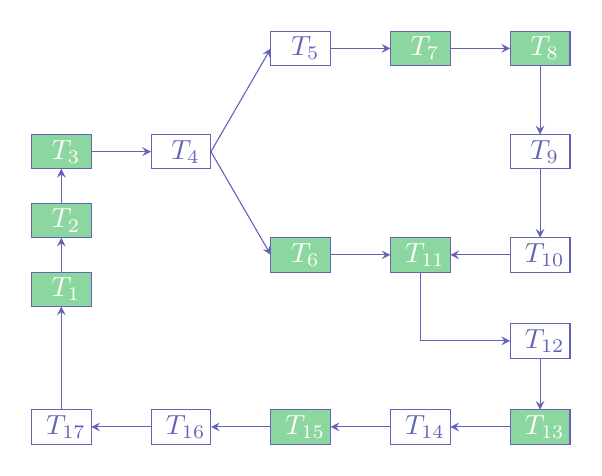
\begin{tikzpicture}[scale=0.38,yscale=1.15]
				%\draw (1,1) grid (19,13);
				\draw[hoccungpi](1,1) rectangle (3,2);
				\draw[hoccungpi](2,1.5) node[] {{ $T_{17}$}};
				\fill[diendantoanhoc!60] (1,5) rectangle (3,6);
				\draw[hoccungpi] (1,5) rectangle (3,6);
				\draw[hoccungpi](2,5.5) node[white] {{ $T_{1}$}};
				\fill[diendantoanhoc!60](1,7) rectangle (3,8);
				\draw[hoccungpi](1,7) rectangle (3,8);
				\draw[hoccungpi](2,7.5) node[white] {{ $T_{2}$}};
				\fill[diendantoanhoc!60] (1,9) rectangle (3,10);
				\draw[hoccungpi] (1,9) rectangle (3,10);
				\draw[hoccungpi] (1,9) rectangle (3,10);
				\draw[hoccungpi](2,9.5) node[white] {{ $T_{3}$}};
				\draw[hoccungpi](5,9) rectangle (7,10);
				\draw[hoccungpi](6,9.5) node[] {{ $T_{4}$}};
				\draw[hoccungpi](5,1) rectangle (7,2);
				\draw[hoccungpi](6,1.5) node[] {{ $T_{16}$}};
				\fill[diendantoanhoc!60](9,1) rectangle (11,2);
				\draw[hoccungpi](9,1) rectangle (11,2);
				\draw[hoccungpi](10,1.5) node[white] {{ $T_{15}$}};
				\fill[diendantoanhoc!60] (9,6) rectangle (11,7);
				\draw[hoccungpi] (9,6) rectangle (11,7);
				\draw[hoccungpi](10,6.5) node[white] {{ $T_{6}$}};
				\draw[hoccungpi](9,12) rectangle (11,13);
				\draw[hoccungpi](10,12.5) node[] {{ $T_{5}$}};
				\draw[hoccungpi](13,1) rectangle (15,2);
				\draw[hoccungpi](14,1.5) node[] {{ $T_{14}$}};
				\draw[hoccungpi] (13,6) rectangle (15,7);
				\fill[diendantoanhoc!60] (13,6) rectangle (15,7);
				\draw[hoccungpi] (13,6) rectangle (15,7);
				\draw[hoccungpi](14,6.5) node[white] {{ $T_{11}$}};
				\fill[diendantoanhoc!60] (13,12) rectangle (15,13);
				\draw[hoccungpi] (13,12) rectangle (15,13);
				\draw[hoccungpi](14,12.5) node[white] {{ $T_{7}$}};
				\fill[diendantoanhoc!60] (17,12) rectangle (19,13);
				\draw[hoccungpi] (17,12) rectangle (19,13);
				\draw[hoccungpi](18,12.5) node[white] {{ $T_{8}$}};
				\draw[hoccungpi](17,9) rectangle (19,10);
				\draw[hoccungpi](18,9.5) node[] {{ $T_{9}$}};
				\draw[hoccungpi](17,6) rectangle (19,7);
				\draw[hoccungpi](18,6.5) node[] {{ $T_{10}$}};
				\draw[hoccungpi](17,3.5) rectangle (19,4.5);
				\draw[hoccungpi](18,4) node[] {{ $T_{12}$}};
				\fill[diendantoanhoc!60] (17,1) rectangle (19,2);
				\draw[hoccungpi] (17,1) rectangle (19,2);
				\draw[hoccungpi](18,1.5) node[white] {{ $T_{13}$}};
				\draw[hoccungpi,-stealth] (2,2) -- (2,5);
				\draw[hoccungpi,-stealth] (2,6) -- (2,7);
				\draw[hoccungpi,-stealth] (2,8) -- (2,9);
				\draw[hoccungpi,-stealth] (3,9.5) -- (5,9.5);
				\draw[hoccungpi,-stealth] (7,9.5) -- (9,12.5);
				\draw[hoccungpi,-stealth] (7,9.5) -- (9,6.5);
				\draw[hoccungpi,-stealth] (11,12.5) -- (13,12.5);
				\draw[hoccungpi,-stealth] (11,6.5) -- (13,6.5);
				\draw[hoccungpi,-stealth] (15,12.5) -- (17,12.5);
				\draw[hoccungpi,-stealth] (18,12) -- (18,10);
				\draw[hoccungpi,-stealth] (18,9) -- (18,7);
				\draw[hoccungpi,-stealth] (17,6.5) -- (15,6.5);
				\draw[hoccungpi,-stealth] (14,6) --(14,4)-- (17,4);
				\draw[hoccungpi,-stealth] (18,3.5) -- (18,2);
				\draw[hoccungpi,-stealth] (17,1.5) -- (15,1.5);
				\draw[hoccungpi,-stealth] (13,1.5) -- (11,1.5);
				\draw[hoccungpi,-stealth] (9,1.5) -- (7,1.5);
				\draw[hoccungpi,-stealth] (5,1.5) -- (3,1.5);
			\end{tikzpicture}
			\caption{\small\textit{\color{hoccungpi}(Các mệnh đề $T_i$ được tô màu xanh là các bất đẳng thức cổ điển, thường được sử dụng.)}}
			\vspace*{-10pt}
		\end{figure}
		Bạn đọc có thể thử sức mình bằng cách tự chứng minh các mũi tên $(T_i)\Rightarrow (T_{j})$ trong sơ đồ trên hoặc tham khảo bài viết [$2$]. (Bạn đọc sẽ tìm thấy trong tài liệu đã dẫn một mạch dài hơn của các bất đẳng thức tương đương với bất đẳng thức Bernoulli). Dưới đây, để minh họa, người viết chỉ điểm qua chứng minh mũi tên $(T_{17}) \Rightarrow (T_{1}).$  Xét số nguyên dương $n$ và số thực $x>0$. Ta có:
		\begin{align*}
			&\dfrac{{{x^{n + 1}} - 1}}{{n + 1}} - \dfrac{{{x^n} - 1}}{n} \\
			= &\dfrac{{x - 1}}{{n(n + 1)}}\left( {n{x^n} - {x^{n - 1}} - {x^{n - 2}} -  \ldots  - 1} \right)\\
			= &\dfrac{{{{(x - 1)}^2}}}{{n(n + 1)}}\left[ {x^{n - 1}} + \left( {{x^{n - 1}} + {x^{n - 2}}} \right) +  \ldots \right. \\
			& \left.+ \left( {{x^{n - 1}} + {x^{n - 2}} +  \ldots  + 1} \right) \right].
		\end{align*}
		Hệ thức trên đây, kết hợp với lập luận bằng quy nạp, dẫn đến
		\begin{align*}
			\frac{{{x^m} - 1}}{m} \geq \frac{{{x^n} - 1}}{n},
		\end{align*}
		với mọi số nguyên dương $m \geq n$. Thay $x^n$ bằng $x$ và $r= \frac{n}{m}$ vào bất đẳng thức vừa thu được, ta có
		\begin{align*}
			{x^r} - 1 \geq  r\left( {x - 1} \right).
		\end{align*}
		Bất đẳng thứuc này đúng với mọi số hữu tỷ $r \geq 1$ và  số thực $x>0$. Lại vì tập các số hữu tỷ
		lớn hơn hoặc bằng $1$ trù mật trong tập các số thực lớn hơn hoặc bằng $1$ nên ta có thể kết luận rằng
		\begin{align*}
			{x^{\alpha} } - 1 \geq  \alpha \left( {x - 1} \right)
		\end{align*}
		với mọi số thực $\alpha \geq 1,x>0$. Thay $x$ bởi $x+1$ ta có bất đẳng thức $(T_1)$. 
		\vskip 0.1cm
		$\pmb{2.}$ \textbf{\color{hoccungpi}Nét đẹp qua phép chứng minh}
		\vskip 0.1cm
		Một lời giải hay, đáng học hỏi chưa hẳn là một lời giải ngắn gọn. Bởi vì điểm hay có thể đến từ ý tưởng hoặc từ kỹ thuật xử lý bài toán (kéo theo là lời giải có thể tương đối dài hoặc không đơn giản). Trong mục này, mời bạn đọc đến với những lời giải như vậy.
		\vskip 0.1cm
		\textbf{\color{hoccungpi}Ví dụ} $\pmb{1.}$
		\textit{Ta nhắc lại hai bất đẳng thức sau:
		\vskip 0.1cm
		$\bullet$ \textbf{\color{hoccungpi}(AM -- GM)} Với mọi số thực dương $a_1, a_2, \ldots, a_n$, ta có
		\begin{align*}
			\dfrac{a_1+a_2+\cdots+a_n}{n} \geq \sqrt[n]{a_1a_2\cdots a_n}.
		\end{align*}
		$\bullet$ \textbf{\color{hoccungpi}(Bất đẳng thức Bernoulli cơ bản)} Với mọi số tự nhiên $n$ và số thực dương $x$, ta có
		\begin{align*}
			x^n \geq 1+n(x-1).
		\end{align*}	
		$a)$ Sử dụng bất đẳng thức AM -- GM, hãy chứng minh bất đẳng thức Bernoulli cơ bản.
		\vskip 0.1cm
		$b)$ Sử dụng bất đẳng thức Bernoulli cơ bản, hãy chứng minh bất đẳng thức AM -- GM.}
		\vskip 0.1cm
		\textit{Lời giải.}
		$a)$ Với $n=0,1$ thì bất đẳng thức Bernoulli cơ bản là hiển nhiên vì nó trở thành đẳng thức. Giả sử $n \geq 2$. Ta xét hai trường hợp 
		\vskip 0.1cm
		$\bullet$ Với $0<x \le 1-\dfrac{1}{n}$ thì bất đẳng thức là hiển nhiên do vế trái dương trong khi vế phải không dương.
		\vskip 0.1cm
		$\bullet$ Với $x>1-\dfrac{1}{n}$, áp dụng bất đẳng thức AM -- GM, ta có
		\begin{align*}
			{x^n}{\rm{ }} &= {\left\{ {\frac{{[1 + n(x - 1)] + \overbrace {1 +  \ldots  + 1}^{n - 1}}}{n}} \right\}^n} \\
			&\ge [1 + n(x - 1)] \cdot 1 \cdot  \ldots  \cdot 1 = 1 \!+\! n(x \!-\! 1).
		\end{align*}
		Ta chứng minh xong bất đẳng thức Bernoulli cơ bản.
		\vskip 0.1cm	
		$b)$ Đặt
		\begin{align*}
			A_n=\dfrac{a_1+a_2+\cdots+a_n}{n},
		\end{align*}
		trong đó $a_1, a_2, \ldots$ là các số thực dương. 
		Trước hết, với $n=1$ thì bất đẳng thức cần chứng minh là tầm thường 
		Xét trường hợp $n \geq 2$. Áp dụng bất đẳng thức Bernoulli, ta có
		\begin{align*}
			\left(\frac{A_{n}}{A_{n-1}}\right)^{n} & \geq 1+n\left(\frac{A_{n}}{A_{n-1}}-1\right) \\
			&=\frac{A_{n-1}+n A_{n}-n A_{n-1}}{A_{n-1}} \\
			&=\frac{n A_{n}-(n-1) A_{n-1}}{A_{n-1}}=\frac{a_{n}}{A_{n-1}}.
		\end{align*}
		Hay nói cách khác,
		\begin{align*}
			A_{n}^{n} \geq a_{n} \cdot A_{n-1}^{n-1}.
		\end{align*}		
		Áp dụng liên tục các bất đẳng thức như vậy, ta thu được
		\begin{align*}
			A_{n}^{n}  &\geq a_{n} \cdot A_{n-1}^{n-1} \geq a_{n} \cdot a_{n-1} \cdot A_{n-2}^{n-2}  \\
			&\geq \cdots \geq a_{n} \cdot a_{n-1} \cdots a_{3} \cdot A_{2}^{2} \\
			&\geq a_{n} \cdot a_{n-1} \cdots a_{3} \cdot a_2 \cdot a_1.
		\end{align*}
		Thế nhưng bất đẳng thức $A_n^n \geq a_1a_2 \cdots a_n$ tương đương với $\dfrac{a_1+a_2+\cdots+a_n}{n} \geq \sqrt[n]{a_1a_2\cdots a_n}$ nên bất đẳng thức AM -- GM được chứng minh.
		\vskip 0.1cm
		\textbf{\color{hoccungpi}Ví dụ} $\pmb{2.}$ \textit{Cho số thực $x>-1$ và số nguyên $k$. Chứng minh rằng $(1+x)^{k} \geq 1+ k x.$}
		\vskip 0.1cm
		 Lưu ý: trong ví dụ trên, số nguyên $k$ có thể âm.
		\vskip 0.1cm
		Với mỗi $x>-1$ cố định, ta xét hàm $\mathscr{B}$  sau đây:
		\begin{align*}
			\mathscr{B}: \mathbb{Z} & \rightarrow \mathbb{R} \\
			k&  \mapsto (1+x)^{-k}(1+k x).
		\end{align*}
		Có thể thấy rằng  $\mathscr{B}(0)= \mathscr{B}(1)=1$. 
		Ta sẽ chứng minh $1$ cũng chính là giá trị lớn nhất của $\mathscr{B}$, từ đó ta thu được kết luận của bài toán. Ta có
		\begin{align*}
			&\mathscr{B}(k)-\mathscr{B}(k-1) \\
			=&\frac{1+k x}{(1+x)^{k}}-\frac{1+(k-1) x}{(1+x)^{k-1}} \\
			=&\frac{1\!+\!k x\!-\![1\!+\!(k\!-\!1) x](1\!+\!x)}{(1\!+\!x)^{k}}=\frac{(1-k) x^{2}}{(1+x)^{k}}.
		\end{align*}
		Vì thế $\mathscr{B}(k)-\mathscr{B}(k-1) \ge 0$ nếu $k\le 0$ và $\mathscr{B}(k)-\mathscr{B}(k-1) \le 0$ nếu $k\ge 2$.
		Ta suy ra giá trị lớn nhất của
		$\mathscr{B}$ là $1$ và do đó chứng minh hoàn tất.
		\vskip 0.1cm
		\textbf{\color{hoccungpi}Ví dụ $\pmb{3.}$ (Bất đẳng thức Bernoulli cho số mũ nằm trong khoảng $\pmb{(0;1)}$).}
		\textit{Cho các số thực $x>-1$ và $0<\alpha <1$. Chứng minh rằng}
			$(1+x)^{\alpha} \le 1+ \alpha x.$
		\vskip 0.1cm
		\textit{Lời giải.} Ta xét tập hợp $T$ sau đây:
		\begin{align*}
			&T=\{\alpha \in (0;1): \forall \,\,y>-1 \\
			&\textrm{ thì } (1+y)^{\alpha} \le 1+ \alpha y\}.
		\end{align*}
		Trước tiên, ta sẽ chứng minh $T$ có ba tính chất sau:
		\vskip 0.1cm
		$(1)$ $\dfrac{1}{2} \in T$.
		\vskip 0.1cm
		$(2)$ Nếu $\alpha \in T$ thì $1-\alpha \in T$.
		\vskip 0.1cm
		$(3)$ Nếu $\alpha, \beta \in T$ thì $\alpha \beta \in T$. Hơn nữa, nếu $\alpha + \beta<1$ thì $\alpha + \beta\in T$.
		\vskip 0.1cm
		Thật vậy,
		\vskip 0.1cm 
		$(1)$ Trước hết ta thấy rằng $\left(1+\frac{y}{2}\right)^{2}=1+y+\frac{y^{2}}{4} \geq 1+y $, cho nên $1+\dfrac{y}{2} \geq  (1+y)^{\frac{1}{2}}$. Hay nói cách khác $\dfrac{1}{2} \in T$.
		\vskip 0.1cm 
		$(2)$ Giả sử $\alpha \in T$. Với mọi $y>-1$ ta có
		\begin{align*}
			\frac{-y}{1+y}=-1+\frac{1}{1+y}>-1.
		\end{align*}
		Từ đó ta được
		\begin{align*}
			(1+y)^{1-\alpha}&=(1+y)\left(1+\frac{-y}{1+y}\right)^{\alpha} \\
			&\le (1+y)\left(1+\frac{-\alpha y}{1+y}\right) \\
			&=1+(1-\alpha) y .
		\end{align*}
		Như vậy $1- \alpha \in  T$.
		\vskip 0.1cm
		$(3)$ Giả sử $\alpha, \beta \in T$ với $0<\alpha < \beta <1$. Khi~đó:
		\begin{align*}
			(1\!\!+\!\!y)^{\alpha  \beta}\!=\!\left[(1\!\!+\!\!y)^{\alpha}\right]^{\beta} \!\!\leq\!\! (1\!\!+\!\alpha y)^{\beta} \!\!\le\!\! 1\!\!+\!\alpha  \beta y.
		\end{align*}
		Tức là $\alpha \beta \in T$. Hơn nữa,
		\begin{align*}
			&(1+y)^{\alpha+\beta} \\
			=&(1+y)^{\alpha}(1+y)^{\beta} \leq (1+\alpha y)(1+\beta y) \\
			=&1+(\alpha+\beta) y+(\alpha  \beta) y^{2} \\
			=&\left(\!1\!+\!\frac{\alpha+\beta}{2} y\right)^{2}\!+\!\left[\alpha  \beta\!-\!\left(\frac{\alpha\!+\!\beta}{2}\right)^{2}\right] y^{2} \\
			\leq&\left(\!1+\frac{\alpha+\beta}{2} y\right)^{2}.
		\end{align*}
		Tức là
		\begin{align*}
			(1+y)^{\frac{\alpha+\beta}{2}} \leq 1+\frac{\alpha+\beta}{2} y.
		\end{align*}
		Như vậy ta được $\dfrac{\alpha +\beta }{2} \in T.$
		\vskip 0.1cm
		Tiếp theo, bằng phương pháp quy nạp theo $n,$ và sử dụng các tính chất $(1)$ và $(3)$, ta chứng minh được rằng: 
		\begin{align*}
			A=\left\{\dfrac{m}{2^n}:m,n \in \mathbb{N}^*,m<2^n\right\} \subseteq T.
		\end{align*}
		Cuối cùng, vì $A$ trù mật trong $(0;1)$ nên $T$ cũng trù mật trong $(0;1)$. Từ đây, bằng cách lập luận dựa vào tính chất liên tục, ta thấy rằng $T=(0,1)$. (Cụ thể, với một dãy số $\alpha_i\in T$ mà $\lim\alpha_i= \alpha$ thì $\alpha \in T$).
		Suy ra với mọi số thực $0<\alpha <1$ và mọi số thực $x>-1$ thì
		\begin{align*}
			(1+x)^{\alpha} \le 1+ \alpha x.
		\end{align*}
			Chứng minh hoàn tất.
		\vskip 0.1cm
		$\pmb{3.}$ \textbf{\color{hoccungpi}Bất đẳng thức Bernoulli qua một số bài toán Olympic}
		\vskip 0.1cm
		Bất đẳng thức Bernoulli khi áp dụng cũng đòi hỏi một số kỹ thuật nhất định. Mời bạn đọc khám phá chúng qua các bài toán sau.
		\vskip 0.1cm
		\textbf{\color{hoccungpi}Bài tập $\pmb{1}$ (Olympic New Zealand  năm $\pmb{2019}$).}
		\textit{Cho $a,b,c$ là các số thực dương có tổng bằng $3$. Chứng minh rằng:}
		\begin{align*}
			a^a + b^b + c^c \ge 3.
		\end{align*}
		\textbf{\color{hoccungpi}Bài tập $\pmb{2.}$ (Olympic Nhật Bản năm $\pmb{2005}$).}
		\textit{Cho $a, b, c$ là các số thực dương có tổng bằng $1$. Chứng minh rằng:}
		\begin{align*}
			a \sqrt[3]{\!1\!+\!b\!-\!c}\!+\!b \sqrt[3]{\!1\!+\!c\!-\!a}\!+\!c \sqrt[3]{\!1\!+\!a\!-\!b} \!\leq\! 1 .
		\end{align*}
		\textbf{\color{hoccungpi}Bài tập $\pmb{3.}$ (Dự tuyển kỳ thi IMO năm $\pmb{2004}$).}
		\textit{Cho $a,b,c$ là các số thực dương thỏa mãn $ab+bc+ca=1$. Chứng minh rằng:}
		\begin{align*}
			\sqrt[3]{\frac{1}{a}+6 b}+\sqrt[3]{\frac{1}{b}+6 c}+\sqrt[3]{\frac{1}{c}+6 a} \leq \frac{1}{a b c}.
		\end{align*}
		\textbf{\color{hoccungpi}Bài tập $\pmb{4.}$ (Olympic Bắc Trung Quốc  năm $\pmb{2009}$).}
		\textit{Cho $x,y,z$ là các số thực dương thỏa mãn $ x^2+y^2+z^2 = 3.$ Chứng minh rằng:}
		\begin{align*}
				&\dfrac{{{x^{2009}} - 2008(x - 1)}}{{y + z}} + \dfrac{{{y^{2009}} - 2008(y - 1)}}{{x + z}} \\
				&+ \dfrac{{{z^{2009}} - 2008(z - 1)}}{{x + y}} \ge \dfrac{1}{2}(x + y + z).
		\end{align*}
		\textbf{\color{hoccungpi}Bài tập $\pmb{5.}$ (Kỳ thi tuyển chọn đội tuyển Đài Loan năm $\pmb{2016}$).}
		\vskip 0.1cm
		\textit{Cho $a,b,c$ là các số thực không âm thỏa mãn:
		\begin{align*}
			(a+b)(b+c)(c+a) \neq 0.
		\end{align*}
		Tìm giá trị nhỏ nhất của biểu thức:}
		\begin{align*}
			P=&{(a + b + c)^{2016}}\left(\frac{1}{{{a^{2016}} + {b^{2016}}}}\right.\\
			 &\left.+ \frac{1}{{{b^{2016}} + {c^{2016}}}} + \frac{1}{{{c^{2016}} + {a^{2016}}}}.\right)
		\end{align*}
		\textbf{\color{hoccungpi}Bài tập $\pmb{6.}$ (IMO Shortlist năm $\pmb{2001}$).} \textit{Cho $\{a_n\}$ là một dãy các số thực dương. Chứng minh rằng có vô số $n$ sao cho:}
		\begin{align*}
			1 + a_n > a_{n-1} \sqrt[n]{2}.
		\end{align*}
		\textbf{\color{hoccungpi}Bài tập $\pmb{7.}$ (IMO Shortlist năm $\pmb{2017}$).}
		\textit{Cho $a_1,a_2,\cdots,a_n,k,M$ là các số nguyên dương sao cho: 
		\begin{align*}
			\frac{1}{a_1}\!+\!\frac{1}{a_2}\!+\!\cdots\!+\!\frac{1}{a_n}\!=\!k\,\,\text{ và }\,\, a_1a_2\cdots a_n=M.
		\end{align*}
		Chứng minh rằng nếu $M>1$ thì
		$M(x+1)^k <(x+a_1)(x+a_2)\cdots (x+a_n)$ với mọi $ x>0.$}
		\vskip 0.1cm
		\textbf{\color{hoccungpi}Lời kết}
		\vskip 0.1cm
		Việc nhìn lại các bất đẳng thức và tìm ra sợi dây liên kết giữa chúng cũng là một cách học bất đẳng thức  thú vị. Chắc hẳn những sợi dây như vậy sẽ còn rất nhiều, chúng đang chờ bạn đọc khám phá.  Cuối cùng, người viết gửi lời cảm ơn đến tác giả Trần Nam Dũng đã có bài viết gợi mở cho bài viết này, và đến người phản biện vì những góp ý bổ ích cho bài viết.
		\vskip 0.1cm
		\textbf{\color{hoccungpi}Tài liệu tham khảo.}
		\vskip 0.1cm
		[$1$] Trần Nam Dũng, \textit{Bất đẳng thức Bernoulli}. Tạp chí Pi, số $10$ năm $2021$. 
		\vskip 0.1cm
		[$2$] Yuan--Chuan Li, Cheh--Chih Yeh. \textit{Some Equivalent Forms of Bernoulli's Inequality: A Survey}.  Applied Mathematics, $2013$.
		\vskip 0.1cm
		[$3$] Maligranda, L. \textit{The AM--GM Inequality is Equivalent to the Bernoulli Inequality}. Math Intelligencer $34$, $1-2$ ($2012$).
\end{multicols}
%	 \newpage